\documentclass[UTF8,11pt]{ctexart}
\usepackage[a4paper,margin=2.2cm]{geometry}
\usepackage{amsmath,amssymb,amsthm,mathtools,bm}
\usepackage[dvipsnames]{xcolor}
\usepackage{enumitem,booktabs,microtype,tcolorbox,fancyhdr,titlesec,array,lastpage}
\tcbuselibrary{breakable}
\usepackage{longtable,graphicx,float,doi}
\usepackage{tikz}
\usetikzlibrary{arrows.meta,positioning}
\usepackage{hyperref}
\usepackage{bookmark}
\hypersetup{colorlinks=true,linkcolor=MidnightBlue,urlcolor=MidnightBlue,citecolor=MidnightBlue,
 pdftitle={Zeros of polyanalytic polynomials: exact local fibers and sharp constructions},pdfauthor={Prepared for Teng Zhang}}
\setlength{\parindent}{2em}
\setlength{\parskip}{0.35em}
\linespread{1.15}
\setlength{\headheight}{15pt}
\setlength{\emergencystretch}{2.5em}
\raggedbottom
\titleformat{\section}{\Large\bfseries\color{MidnightBlue}}{\thesection}{0.6em}{}
\titleformat{\subsection}{\large\bfseries\color{MidnightBlue}}{\thesubsection}{0.6em}{}
\newtheorem{thm}{Theorem}[section]
\newtheorem{prop}[thm]{Proposition}
\newtheorem{lem}[thm]{Lemma}
\newtheorem{cor}[thm]{Corollary}
\newtheorem{prob}[thm]{Problem}
\newtheorem{conj}[thm]{Conjecture}
\theoremstyle{definition}
\newtheorem{rem}[thm]{Remark}
\newtheorem{defin}[thm]{Definition}
\newtheorem{eg}[thm]{Example}
\numberwithin{equation}{section}
\newcommand{\C}{\mathbb C}\newcommand{\R}{\mathbb R}
\newcommand{\N}{\mathbb N}\newcommand{\Z}{\mathbb Z}\newcommand{\Q}{\mathbb Q}
\newcommand{\CP}{\mathbb {CP}}\newcommand{\cP}{\mathcal P}
\newcommand{\cA}{\mathcal A}\newcommand{\A}{\mathcal A}
\newcommand{\HH}{\mathcal H}\newcommand{\Ecal}{\mathcal E}
\newcommand{\Tcal}{\mathcal T}\newcommand{\Ccal}{\mathcal C}
\newcommand{\eps}{\varepsilon}\newcommand{\ep}{\varepsilon}
\newcommand{\dd}{\,d}\newcommand{\av}{\textup{author version}}
\newcommand{\norm}[1]{\left\lVert #1\right\rVert}
\newcommand{\ip}[2]{\left\langle #1,#2\right\rangle}
\DeclareMathOperator{\Rea}{Re}\DeclareMathOperator{\Ima}{Im}
\DeclareMathOperator{\rank}{rank}\DeclareMathOperator{\tr}{tr}\DeclareMathOperator{\Tr}{Tr}
\DeclareMathOperator{\ord}{ord}\DeclareMathOperator{\Fix}{Fix}
\DeclareMathOperator{\sgn}{sgn}\DeclareMathOperator{\wind}{wind}
\DeclareMathOperator{\Res}{Res}\DeclareMathOperator{\Disc}{Disc}
\DeclareMathOperator{\rad}{rad}\DeclareMathOperator{\spanC}{span_{\C}}
\pagestyle{fancy}\fancyhf{}
\fancyhead[L]{\small Polyanalytic zeros: proofs and audit}
\fancyhead[R]{\small\thepage/\pageref{LastPage}}
\fancyfoot[C]{\small Consolidated research note}
\setlist{itemsep=0.25em,topsep=0.35em}
\renewcommand{\contentsname}{Contents}
\renewcommand{\refname}{References}
\renewcommand{\figurename}{Figure}
\renewcommand{\tablename}{Table}
\renewcommand{\proofname}{Proof}
\renewcommand{\appendixname}{Appendix}
\begin{document}
\begin{titlepage}
\centering
\vspace*{0.5cm}
{\Huge\bfseries\color{MidnightBlue} Zeros of polyanalytic\\[0.25em] polynomials\par}
\vspace{0.6cm}
{\Large A consolidated research note,\\[0.25em] with exact local fibers and a linear sharp region\par}
\vspace{0.7cm}
{\large Prepared for Teng Zhang\par}
\vspace{0.5cm}
{\large October 8, 2026\par}
\vfill
\begin{tcolorbox}[colback=MidnightBlue!4,colframe=MidnightBlue!50,sharp corners,boxrule=0.5pt,width=0.94\textwidth,fontupper=\small]
\textbf{Abstract.}
We study distinct zeros of polynomials in $z$ and $\bar z$ with
prescribed analytic and conjugate degrees. An unrestricted splitting
recurrence and translated coefficient reduction prove
$E_{kr,k(2r+1)}=k^2(2r+1)^2$ for all $r,k\ge1$.
Inversion and circle addition give
$M_{m,n}=m^2+n^2$ throughout $m<n\le3m$, except for the line
$n=3m-1$, whose first three cases are known separately.
The main families have integer extremizers with maximal real-axis
counts. The bound $\min\{m^2+n^2,(4m+1)n-5m\}$ and radial
constructions identify the sharp fixed-$m$ asymptotic coefficient.
We also classify all fibers of the local splitting model, determine
attainable-count spectra, and prove the harmonic distinct minimum
$n-m+1$ with a sharp total-fiber-deficit bound.
For $z^n-z^k+\varepsilon\bar z^m$, $1\le k<m<n$, a monotone
critical-value argument gives the complete parameter-plane count,
the exact maximum $n+2m+k+1$, and the uniform integer maximizer
$\varepsilon=3$. The endpoint $k=m$ has a separate exact maximum
and spectrum governed by $\gcd(n-m,2m)$, including every
unit-circle fiber. Divisor formulas determine the sharp three-term
maxima in conjugate degrees one and two, including the distinct
answer obtained by requiring every zero to be nondegenerate.
Sharp factorization deficits classify reducible
equality cases and pure-head factor-count strata. Optimizing
completion over the proved cone further improves pure-head
lower bounds. These family maxima, optimal constants, and
asymptotic statements are distinguished from the global
bidegree endpoints that remain unresolved. A restriction-map
construction also proves $M_{2,n}=9n-10$ for every even
$n\ge10$, reduces the large odd-degree gap to two,
and completely determines the degree tradeoff for at least
eighty-four zeros: $(m,n)=(1,18),(2,12),(3,10)$.
A critical shared seed further reduces the degree-seven
endpoint to $E_{2,7}\in\{45,47\}$.
\end{tcolorbox}
\vspace{0.6cm}
{\small Mathematics Subject Classification (2020): 30C15; 14P05, 57R40, 65G20.\par}
{\small Keywords: polyanalytic polynomial; harmonic polynomial; zero counting; extremal construction; exact certification.\par}
\vfill
{\small This is a consolidation of the research record, not a claim of journal acceptance or external peer review.\par}
\end{titlepage}
\begingroup\small\setlength{\parskip}{0pt}\linespread{0.93}\selectfont\tableofcontents\endgroup
\newpage
\section{The problem, the literature, and the scope of the conclusions}\label{sec:intro}

Allowing a polynomial to depend on both $z$ and $\bar z$ changes its zero set fundamentally. It may have no zeros, finitely many isolated zeros, or an entire real algebraic arc of zeros. Even when the zero set is finite, an analytic degree is not by itself the total degree, and different coefficient spaces have different extremal counts. The purpose of this note is to put the successive results of the research discussion into one proof structure, with those distinctions made explicit.

\subsection{Notation and the original question}\label{sec:notation}
Throughout, the independent analytic variable is written first:
\[
 f\in\C[z,w],\qquad F_f(z)=f(z,\bar z),\qquad
 f^*(z,w)=\overline{f(\bar w,\bar z)},\qquad N(f)=\#F_f^{-1}(0).
\]
The ordered bidegree is $(\deg_w f,\deg_z f)=(m,n)$: the conjugate degree is listed first, although $z$ is written first in $f(z,w)$. For a multivariate polynomial, an unqualified $\deg$ denotes total degree. The notation $N(F)$ is used interchangeably with $N(f)$ when $F=F_f$. Every zero count in this note counts distinct points, unless a local algebraic multiplicity is explicitly mentioned. We write $f^\#(w)=\overline{f(\bar w)}$ only for a univariate polynomial.

The original rectangular problem is the following.
\begin{prob}\label{core:problem}
Fix $m\ge1$. For polynomials of bidegree $(m,n)$, $n>m$, with $N(f)<\infty$, does there exist a bound $N(f)\le C_1(m)n+C_2(m)$ independent of the coefficients and of $n$?
\end{prob}

As of the source check for this note, Eremenko's maintained problem list
marks the non-holomorphic-equation estimate as solved using AI by reduction
to the Thom genus inequality \cite{Ere26b}. That status notice is not a
replacement for the proof below, and does not certify the stronger
finite-degree assertions in this research record.

This is the polynomial conjecture on page~1 of Eremenko's note dated September~7, 2026 \cite[p.~1]{Ere26}, with the finiteness assumption stated explicitly. It is not the elliptic-system question on the following pages of that note. Two corrections are necessary when quoting the source literally. First, without finiteness, $z^{n-1}(zw-1)$ is a counterexample: its real-slice zero set contains the unit circle. Second, the rough $n^2$ estimate printed there is not valid for a general rectangle of bidegrees. For $0<a<1$,
\[
 f(z,w)=(z^2-a^2)w-z
\]
has bidegree $(1,2)$ and exactly the five zeros
\[
 0,\quad \pm\sqrt{1+a^2},\quad \pm i\sqrt{1-a^2}.
\]
For a nonzero zero, division by $z$ gives $|z|^2-1=a^2\bar z/z$; its real and imaginary parts give precisely the listed possibilities. The correct rectangular intersection bound is $m^2+n^2$. The repeated symbol $C_1$ in the constant term of Eremenko's display is immaterial to the qualitative growth question; we use the two-constant notation of Problem~\ref{core:problem}.

To avoid transferring a sharp result to a larger class without proof, we use the following separate quantities:
\begin{longtable}{@{}>{\raggedright\arraybackslash}p{0.18\textwidth}>{\raggedright\arraybackslash}p{0.76\textwidth}@{}}
\toprule
Notation & Coefficient class over which the maximum is taken \\
\midrule
\endhead
$M_{m,n}$ & Exact bidegree $(m,n)$ and finite zero set. No bound on total degree other than $m+n$.\\
$E_{m,n}$ & $cz^n+\sum_{i+j\le n-1,\ j\le m}c_{ij}z^i\bar z^j$, where $c\ne0$. Its highest homogeneous part is purely analytic.\\
$M^{\mathrm{harm}}_{m,n}$ & $p(z)+\overline{q(z)}$, where $\deg p=n>\deg q=m$.\\
$S_{m,n}$ & The restricted harmonic family $\varepsilon z^n+q(z)+\overline{q(z)}$, where $\varepsilon\ne0$ and $\deg q=m$.\\
$A_{m,n}$ & $\varepsilon z^n+R(x,y)$, where $R\in\R[x,y]$ has total degree $m<n$.\\
$K_{m,n,r}$ & The support-restricted space in Section~\ref{n:sec:support}, with $1\le m<r\le n$.\\
$s_n$ & The least number of nonzero monomials among total-degree-$n$ polynomials with $n^2$ distinct zeros.\\
\bottomrule
\end{longtable}
The notation $\Ecal_{m,n}$ denotes the coefficient space defining $E_{m,n}$. Its conjugate degree is at most $m$; all exact constructions below can be arranged to have degree exactly $m$. The total-degree class $p(z)+Q(z,\bar z)$, $\deg p=n$, $\deg_{\rm tot}Q\le m$, is different from both the rectangular class and $\Ecal_{m,n}$.

\subsection{Established results and exact source locations}\label{sec:history}
The harmonic problem was raised by Sheil-Small in 1992; the contemporary discussion is in Khavinson--\'{S}wi\k{a}tek \cite[pp.~409--410]{KS03}. Wilmshurst proved the quadratic upper bound and constructed extremizers when the smaller degree is one less than the larger \cite[pp.~2077--2080]{Wil98}. Bshouty, Hengartner, and Suez gave an independent extremal construction \cite[pp.~207--218]{BHS95}. Peretz and Schmid independently treated the quadratic zero bound by algebraic methods \cite[pp.~203--208]{PS97}; the original page~204 is also explicitly cited in the proof discussion of \cite[p.~6]{SZ24}. A direct copy of the Peretz--Schmid article was not available in this audit; this attribution and its locator are reported through those authors' published references, not represented as a page-by-page inspection.

For conjugate degree one, Khavinson--\'{S}wi\k{a}tek proved $3n-2$ as an upper bound \cite[Theorem~1, p.~410]{KS03}, and Geyer proved sharpness \cite[Corollary~2, p.~549]{Gey08}. For a rational analytic term of degree $n$, Khavinson--Neumann established $5n-5$ \cite[Theorem~1, \av, p.~1]{KN06}; Rhie's construction gives sharp examples \cite[pp.~3--4]{Rhi03}. Singular zeros and degree-dependent refinements were subsequently treated by Luce--S\`ete--Liesen \cite[Theorem~1.1, \av, p.~2]{LSL15} and Liesen--Zur \cite[Theorem~1.1 and Theorem~3.5, \av, pp.~2, 7]{LZ18}. Lee--Makarov's prescribed-pole construction \cite[Theorem~C, p.~3]{LM14} supplies the sharp degree-dependent endpoint recorded in Section~\ref{n:sec:known}. Those endpoint results are not new here.

Wilmshurst's proposed refinement $3n-2+m(m-1)$ is false in general. Lee, Lerario, and Lundberg constructed counterexamples and explicitly proposed fixed-$m$ linear growth \cite[\av, pp.~1--4]{LLL15}. Their stronger conjecture bounds the number of orientation-reversing zeros by $m(n-1)$ \cite[\av, p.~3]{LLL15}. Neither that conjecture nor the exact unrestricted harmonic maximum is proved below. Khavinson, Lee, and Saez give further constructions and warn, in effect, against assigning at most one zero to each orientation-reversing component \cite[Theorems~2--3, p.~2]{KLS18}. Lee and Saez analyze the regime $m=n-2$ in detail \cite[unnumbered Theorem, \av, p.~1]{LS17}; their count is $n^2-2n+2+4k_{\max}(n)$ with the trigonometric integer $k_{\max}$ defined there, not just $n^2-2n+2$. Their theorem explicitly counts multiplicities, a convention that should not silently be replaced by distinct zeros.

Certified numerical constructions were developed by Hauenstein, Lerario, Lundberg, and Mehta \cite[Section~1.3, \av, p.~3]{HLLM15}. Lundberg's probabilistic construction gives examples with at least $\lceil n\sqrt m\rceil$ zeros \cite[Theorem~1.1, \av, p.~2]{Lun23}. The concrete deterministic question relevant here is in his Section~4.2, page~9 of arXiv:2201.00788v2: can a strategic choice of the coefficients in the monomial-head family produce order $mn$ instead? The exact restricted-family result in Section~\ref{b:sec:harmonic} answers that question, while Section~\ref{h:sec:Cheb} changes the analytic head and improves the constructed linear coefficient.

Average-case asymptotics should be kept separate from worst-case valence.
Lerario--Lundberg establish $n^{3/2}$ growth for the truncated Gaussian
model with $m=\alpha n$, $0<\alpha<1$, and asymptotic $n$ for fixed $m$
\cite[Theorem~1, \av, p.~3]{LL16}. For independent identically distributed
Kac coefficients, Lu--Wang prove bounds of order $n$ when $m=\alpha n$
\cite[Theorem~2.1 and inequalities (2.1)--(2.4), \av, p.~4]{LW25}.
The latter article appeared in 2025, although its accepted author manuscript
was posted to arXiv in September 2026. Neither ensemble estimate is a
coefficient-uniform upper bound on the maximal number of zeros.

For general polyanalytic polynomials, Khavinson, Lundberg, and Perry formulate the bidegree problem and give the coprime intersection estimate $m^2+n^2$ \cite[Problem~1.9 and Proposition~1.10, \av, pp.~3--4]{KLP24}. In the distinct logharmonic subclass with one linear factor, their $3n-1$ estimate is attained by Lazebnik--Lundberg \cite[Theorem~1.3, \av, p.~2]{LL26}. S\`ete--Zur give a systematic account of finiteness, total-degree bounds, possible zero counts, and constructions \cite[Theorems~2.7, 2.12, 2.16 and 4.1, pp.~5--8, 12--14]{SZ24}. Their Remark~4.4 on page~16 conjectures that at least $n$ nonzero coefficients are needed for $n^2$ zeros; Section~\ref{q:sec:sparse} gives a three-term quartic counterexample and proves that degree four is the first failure. Their Section~5 concerns a total-degree-restricted mixed class, not the full rectangle.

The algebraic trace method in Section~\ref{g:sec:gap} builds on Furch\`i's Hermitian trace form \cite[Theorem~3.13, Corollary~3.14, and Lemma~4.3, \av, pp.~9--10, 16--17]{Fur25}. We prove the additional trace identity and isotropic-space estimate needed here. The surface arguments use the Thom genus theorem of Kronheimer--Mrowka \cite[Theorem~1, \av, p.~1]{KM94}; the version allowing only negative ordinary double points is stated explicitly by Orevkov \cite[Theorem~3.1, \av, p.~8]{Ore24}. Finally, separated-coefficient arguments have antecedents in the real-rootedness and tropical Descartes theory of Forsg{\aa}rd--Novikov--Shapiro \cite[Proposition~1 and Section~2, author proof, pp.~2, 4]{FNS17}. That proposition attributes the sign-independent real-rootedness criterion to
Passare--Rojas--Shapiro \cite[Definition~1 and Theorem~1, \av, p.~2]{PRS11}.
We give the elementary sign argument rather than presuppose independence of
the restrictions to different lines.

All references marked ``author version'' use the specific version in the bibliography; other page references use the published pagination. Publication metadata and mathematical locators were checked separately. Standard textbook citations identify the chapters or propositions actually used, but this audit does not claim visual inspection of every page of every cited book. The literature review concerns the zero-counting questions in this research record; it is not a proof of priority against every unpublished manuscript.

\subsection{The principal conclusions}\label{sec:overview}
The first conclusion settles Problem~\ref{core:problem} and identifies its optimal leading constant.
\begin{thm}\label{b:thm:main}
For $n>m\ge1$ and every polynomial of bidegree $(m,n)$ with finite zero set,
\begin{equation}\label{b:eq:mainbound}
 N(f)\le\min\{m^2+n^2,(4m+1)n-5m\}.
\end{equation}
For every fixed $m\ge1$, $\lim_{n\to\infty}M_{m,n}/n=4m+1$.
\end{thm}

The strengthened constructions in Section~\ref{new:sec:twofreq} give the
following additional main conclusions. With
$U_{m,n}=\min\{m^2+n^2,(4m+1)n-5m\}$, every $n>m\ge1$ satisfies
\[
 U_{m,n}-4m(m-1)\le M_{m,n}\le U_{m,n}.
\]
For $n\ge2m+1$ the more precise constructed lower count is
$(4m+1)(n-m)+(3m-n)_+(3m+1-n)_+$.
The exact maximum in the two-frequency family with radial degrees $a,b$
is $k\min\{2(a+b)+1,k+2a-\mathbf1_{2\mid k}\}$ whenever $k+2a>2b$.
Optimizing the unequal radial degrees also proves
$E_{m,4m+2}\ge9m^2+7m+2$ and the general bound
\eqref{new:eq:purelower}. The rectangular and pure-head estimates are
lower bounds for their full spaces; only the stated two-frequency
maximum is asserted to be exact throughout its parameter range.

The finite-degree results now include a linear region of exact rectangular
maxima. The stronger pure-head conclusions have a separate range.
The new recurrence and inversion proof are entirely analytic; part of
the older pure-head boundary $n=2m+2$ retains its certificate dependency.
\begin{thm}\label{d:thm:main}
For $m\ge2$ and $m<n\le2m+2$,
\begin{equation}\label{d:eq:main}
 E_{m,n}=n^2,\qquad M_{m,n}=m^2+n^2.
\end{equation}
The same equalities hold when $n=2m+3$ and $3\mid m$.
More generally, the pure-head equality holds at
\[
 (m,n)=(kr,k(2r+1)),\qquad r\ge1,\quad k\ge1,
\]
and remains valid after increasing $m$ while keeping $m<n$.
For the rectangular class,
\begin{equation}\label{v3:eq:introband}
 M_{m,n}=m^2+n^2\quad
 (1\le m<n\le3m,\ n\ne3m-1).
\end{equation}
The cases $(1,2),(2,5),(3,8)$ also satisfy the rectangular equality.
All these extrema admit Gaussian rational coefficients, exact conjugate
degree $m$, and nondegenerate zeros.
\end{thm}

Theorem~\ref{v3:thm:splitting} removes the earlier restriction
$r\ge k-1$. The translated construction in
Theorem~\ref{v16:thm:borderline} also closes the pure-head boundary
$r=1$: $E_{m,3k}=9k^2$ and $M_{m,3k}=m^2+9k^2$
for $k\le m<3k$.
Theorem~\ref{v3:thm:band} then proves \eqref{v3:eq:introband} by at
most two circle additions. For example, $E_{8,20}=400$,
$M_{8,20}=464$, $E_{4,12}=144$, $M_{4,12}=160$, and
$M_{10,30}=1000$.
At $m=10000$ the proved range beyond $n=2m$ includes every
$1\le d\le9998$ and $d=10000$, replacing the earlier sufficient
range $1\le d\le46$. The line $n=3m-1$, $m\ge4$, remains unresolved
here. The paired-seed construction in Theorem~\ref{v33:thm:129}
strictly improves its first missing lower bound to
$129\le M_{4,11}\le137$. Equality on the rectangular cone
is not asserted for $E$.
Corollary~\ref{v31:cor:minimumdegree} also proves that the conjugate
degrees of the cubic-boundary extremizers are minimal at total
degrees $3,6,\ldots,24$. Reducing the conjugate degree by one
then loses at least six zeros; the possible degree reductions at
$n=10,11,13,27$ remain explicitly bracketed.

For the pure-head class, Corollary~\ref{v16:cor:extension} gives
$E_{m,n}\ge9m^2+n-3m$ when $n\ge3m$, and the uniform
deficit $n^2-E_{m,n}\le4n-6$ throughout $m<n\le3m$.
Thus its quadratic asymptotic bound is sharp on the entire cone.
Theorem~\ref{v38:thm:88} improves the first pure-head case beyond
the cubic boundary to $88\le E_{3,10}\le100$, with an exact
eighty-eight-zero construction and ten real-axis zeros. Total
degree ten and, at that degree, conjugate degree three are minimal
for this target. The global maximum remains open.
The critical-seed construction in Theorem~\ref{v43:thm:45}
improves the smaller endpoint to $E_{2,7}\in\{45,47\}$,
with exactly forty-five regular zeros and seven real-axis zeros.
Total degree seven and conjugate degree two are minimal for
this target. Proposition~\ref{v43:prop:localsharp} also makes
forty-five the sharp maximum throughout a small full coefficient
neighborhood of its critical limiting seed. The global endpoint
forty-seven remains open.
Proposition~\ref{v38:prop:localsharp} proves that $41$ and $88$
are nevertheless the exact maxima in sufficiently small full
coefficient neighborhoods of the two fixed limiting seeds.
Proposition~\ref{v39:prop:fixed41} gives an explicit integer
coefficient table for the forty-one-zero example, with all
$49$ complex intersections certified at fixed parameter values.

The restriction-map construction in
Theorem~\ref{v40:thm:rectangle} closes an infinite family of global
rectangular endpoints: $M_{2,n}=9n-10$ for every even $n\ge10$.
For odd $n\ge13$ it gives $M_{2,n}\in\{9n-12,9n-10\}$;
the smaller cases satisfy $M_{2,8}\in\{60,62\}$,
$65\le M_{2,9}\le71$, and $85\le M_{2,11}\le89$.
Theorem~\ref{v41:thm:purebands} narrows the pure-head gaps
to two in every even degree $n\ge8$ and four in every odd
degree $n\ge9$. In particular, $61\le E_{2,9}\le65$,
$90\le E_{2,12}\le92$, and $115\le E_{2,15}\le119$.
Corollary~\ref{v41:cor:degreewindows} also determines the
minimum degrees for whole intervals of target zero counts.
For the eighty-four-zero threshold,
Corollary~\ref{v40:cor:degree84} determines every minimum
allowed pure degree at a fixed conjugate degree; the complete
undominated choices are $(1,18),(2,12),(3,10)$.

For splitting order two, Lemma~\ref{v15:lem:unitdisk} sharpens
the coefficient stability radius to the optimal value one.
The unadjusted cubic cofactor then gives the explicit analytic
family \eqref{v15:eq:sextic}, proving $E_{2,6}=36$ independently
of the earlier rational-box certificate. The seed and its split
have respectively nine and thirty-six simple zeros; the latter
also attains the real-axis bound of six.

An independent certified contact-six construction attains $39$
zeros in Corollary~\ref{v22:cor:E27}. Its seed has exactly $26$
regular zeros and all
$36$ complex intersections are certified. The fixed choice
$\varepsilon=10^{-24}$ in \eqref{v25:cor:fixed39} also has its
own certificate for all $49$ intersections and exactly $39$ real
zeros. This does not determine the rectangular endpoint $M_{2,7}$.

For splitting order three, Theorem~\ref{v18:thm:shear} determines
the exact shear disk for every real constant term. The canonical
radius is $1-(3/4)^{1/3}$; the unique optimized constant gives
radius $1/4$, with all first-boundary parameters and fold counts
explicitly classified.

Theorem~\ref{v5:thm:fibers} gives the exact number of preimages
of every complex target under the local folding map, including all
degenerate targets. Corollary~\ref{v5:cor:disk} and Lemma~\ref{v28:lem:inradius}
give its unique largest target disk over all complex centers. Dropping an unnecessary constant in the
recurrence upgrades the new families and rectangular cone to real
rational, hence integer, coefficients. The same extremizers attain
the real-axis upper bounds $n$ in the pure-head class and $m+n$
in the rectangular class (Corollary~\ref{v5:cor:realaxis}).
These improvements do not close the remaining global degree gaps.

Theorem~\ref{v6:thm:spectra} upgrades each known maximal count to
a complete spectrum: with nonzero rectangular corner the simple counts
are $n-m,n-m+2,\ldots,M_{m,n}$; in the pure-head class they are
$n,n+2,\ldots,E_{m,n}$. Allowing degeneracies gives every positive
integer up to the respective maximum.
\emph{Exact} positive conjugate degree in the pure-head class instead
gives precisely $2,\ldots,E_{m,n}$ by Theorem~\ref{v7:thm:pureexact}.
The fixed-degree harmonic
no-gap theorem above $n$ is already due to S\`ete--Zur \cite{SZ21}.
Theorem~\ref{v7:thm:minimum} determines the sharp distinct minimum
$n-m+1$ and proves that the total deficit below $n$, summed over
all targets of one harmonic map, is at most $\deg\gcd(p',q')$.
Thus its full distinct spectrum is
$\{n-m+1,\ldots,M^{\mathrm{harm}}_{m,n}\}$; at $m=n-1$ this
is exactly $\{2,\ldots,n^2\}$. Integer trinomials realize its
lower end and have the exact parameter disk in
Theorem~\ref{v7:thm:trinomialradius}. Separately,
Proposition~\ref{v7:prop:completion} improves the pure-head lower
bound to $E_{m,4m+1}\ge10m^2+2m+1$.
Theorem~\ref{v6:thm:cubicradius} also optimizes the entire real
constant-term parameter of the nine-zero cubic, with unique maximal
uniform radius $(5\sqrt5-11)/2$.

Theorem~\ref{v34:thm:nonmultiples} determines the individual
unit-triple power constant in every order not divisible by three,
with all equality traces. Along these orders,
$C_k/k\to\Gamma\approx1.11562380$; the constant $\Gamma$
is characterized exactly in Corollary~\ref{v34:cor:asymptotic}. Proposition~\ref{v35:prop:power1215} also determines
$C_{12}$ and $C_{15}$ and their six equality traces, so every
individual order through seventeen is settled.

The trinomial parameter analysis extends beyond the first transition.
For $1\le k<m<n$, Theorem~\ref{v9:thm:trinomialmaximum} proves
\[
 \max_{\varepsilon\in\C}N(z^n-z^k+\varepsilon\bar z^m)
 =n+2m+k+1,
\]
with the universal integer maximizer $\varepsilon=3$.
Proposition~\ref{v9:prop:allparameters} gives the exact count in
every regular parameter region and at its fold and cusp boundaries.
The full distinct spectrum in this family has step
$\gcd(n-k,m+k)$. The optimal outer radius is at most two.
The endpoint $k=m$ is completed by Theorem~\ref{v10:thm:endpoint}.
Writing $\ell=\gcd(n-m,2m)$, its maximum is $n+m+1$ when
$2m/\ell$ is even and $n+m+\ell+1$ when it is odd.
Its full spectrum and all unit-circle fibers are explicit;
complex parameters sometimes exceed the real-parameter maximum.

There is also a complete sparsity-restricted result in conjugate
degree one. If $D(N)$ is the largest proper divisor of $N$, then
Theorem~\ref{v11:thm:sparsemaximum} proves
\[
 H^{(3)}_{1,n}=n+2+2D(n+1)\qquad(n\ge4).
\]
The low-degree values are $H^{(3)}_{1,2}=4$ and $H^{(3)}_{1,3}=7$.
Thus a harmonic trinomial attains the full $3n-2$ maximum exactly
in degrees $2,3,5$. For $z^n-z^k+\varepsilon\bar z$, $2\le k<n$,
the exact family maximum is $n+2+2\gcd(n+1,k+1)$, with an explicit
open interval of positive rational maximizing parameters.

The support classification now also closes conjugate degree two.
Theorem~\ref{v13:thm:sparsemaximum} proves, for $n\ge7$,
\[
 H^{(3)}_{2,n}=\max\{n+6,n+3+2D(n+2)\},\qquad
 H^{(3),\mathrm{reg}}_{2,n}=n+6.
\]
The four smaller distinct maxima are $9,10,11,13$ in degrees
$3,4,5,6$, and the regular formula holds from degree three.
For even $n\ge8$ the distinct maximum is $2n+5$.
The underlying separated-component theorem gives
$n+m+1+2\gcd(n+m,k+m)$ for $n>k>m$ under the explicit
criterion \eqref{v12:eq:separation}, which always holds for $m=2$.
All nonzero maximizing zeros are regular; the multiple origin
is retained when $m>1$. Separately,
Proposition~\ref{v14:prop:purecontact} strengthens the pure-head
upper bound by $2(q-2m)$ under contact order $q>2m$.
Its maximal-contact degree-one endpoint has sharp value $3n-2$,
including singular members, by Corollary~\ref{v14:cor:sharpcontact}.
The threefold-symmetric contact-five subspace has the smaller sharp
distinct maximum $19$, including singular parameters
(Proposition~\ref{v23:prop:cyclicfive}); an integer example attains it
with all zeros regular.

Factorization now has its own sharp theory. For $n>m\ge2$,
Theorem~\ref{v8:thm:redquadratic} bounds every reducible count by
$n^2+(m-1)^2+1$ and characterizes equality by a conjugate-linear
factor times a saturated neighboring rectangle. For $n\ge m^2+2$,
$M^{\mathrm{red}}_{m,n}=M_{m,n-1}+1$; the reducible fixed-$m$
asymptotic coefficient is also $4m+1$. In the pure-head class,
exact conjugate degree $m$ permits at most $n-m$ factors, and
Theorem~\ref{v8:thm:purefactors} gives sharp factor-count strata.
The three-candidate optimization in Theorem~\ref{v8:thm:completionenvelope}
also improves the pure-head constructions below $n=4m+1$; for example,
$E_{100,399}\ge99005$ instead of the radial count $89799$.

For harmonic polynomials, the strongest general estimates established in the record are most compactly stated together. The endpoints $m=1$ and $m=n-1$ are classical, as explained above.
\begin{thm}\label{core:harmonicbounds}
For $1\le m<n$, put $g=\gcd(m,n)$. Then
\begin{equation}\label{core:harmonicbounds:eq}
 (m+2)n-m-g\le M^{\mathrm{harm}}_{m,n}
 \le\min\left\{n^2-2\left\lfloor\frac{(n-m)^2}{4}\right\rfloor,
 (3m+2)n-m^2-4m-g\right\}.
\end{equation}
Moreover, $M^{\mathrm{harm}}_{1,n}=3n-2$ and $M^{\mathrm{harm}}_{n-1,n}=n^2$.
\end{thm}

In particular $mn\le M^{\mathrm{harm}}_{m,n}\le4mn$ uniformly in both degrees. For fixed $m\ge2$, the lower coefficient in the constructions is $m+2$, whereas the upper coefficient is $3m+2<4m+1$. These are not matching constants. The exact formulas for $S_{m,n}$, $A_{m,n}$, and the cyclic family are separate theorems, not formulas for the unrestricted harmonic maximum.

The proof organization follows dependencies rather than the order of the chat. Sections~\ref{core:algebra}--\ref{b:sec:radial} establish intersection bounds, regularization, the surface argument, and the matching asymptotic construction. Sections~\ref{n:sec:support}--\ref{g:sec:gap} refine the upper bounds. Sections~\ref{b:sec:harmonic}--\ref{q:sec:sparse} treat harmonic, real-valued, and sparse constructions. Sections~\ref{d:sec:seeds}--\ref{v6:sec:spectra} prove the exact finite-degree ranges and their attainable-count spectra. The final sections collect exact certificates, an audit of superseded assertions, and the questions not settled by these arguments.

\begin{tcolorbox}[colback=MidnightBlue!4,colframe=MidnightBlue!50,sharp corners,boxrule=.5pt]
\textbf{Scope of ``sharp.''} An exact maximum for a specified subspace, an optimal asymptotic coefficient, and a full formula for every bidegree are different claims. This note proves the first two in the places explicitly stated. It does not prove $M_{m,n}=\min\{m^2+n^2,(4m+1)n-5m\}$ for every pair, and it does not determine $M_{2,7}$.
\end{tcolorbox}

\section{Intersection bounds and nondegenerate zeros}\label{core:algebra}
The elementary intersection statements in this section will also certify completeness of constructions. They are established before regularization so that later extremal examples do not depend on the surface argument.

At a real-slice point, the real Jacobian is
\begin{equation}\label{core:jacobian}
 J_f=|f_z|^2-|f_w|^2
 =\det\begin{pmatrix}f_z&f_w\\\overline{f_w}&\overline{f_z}\end{pmatrix}.
\end{equation}
A zero is \emph{nondegenerate} if this number is nonzero. We denote the numbers of positive and negative nondegenerate zeros by $N_+(f)$ and $N_-(f)$, and put $N_{\rm nd}=N_++N_-$. Rank zero of the real differential is equivalent to $f_z=f_w=0$.

The following total-degree statement is particularly useful. It also follows from \cite[Corollary~2.14, p.~7]{SZ24} together with local intersection multiplicity.
\begin{lem}\label{d:lem:pure}
If $f=z^N+q(z,w)$ with $\deg_{\rm tot}q<N$, then $(f,f^*)$ is a zero-dimensional complete intersection of length $N^2$. In particular, $N(f)\le N^2$. If $N^2$ distinct real-slice zeros occur, every one is nondegenerate.
\end{lem}
\begin{proof}
In a graded monomial order, the leading monomials are $z^N$ and $w^N$. They are relatively prime, so the two polynomials form a Gr\"obner basis. The residue classes of $z^iw^j$, $0\le i,j<N$, form a basis of the quotient, proving the length assertion and finiteness. Equivalently, the projective curves have no common point at infinity. If $N^2$ distinct real points occur, each local intersection has length one; the two gradients are independent. Its determinant is \eqref{core:jacobian}, which proves the last assertion.
\end{proof}

For the rectangle we remove the common-factor hypothesis explicitly.
\begin{prop}\label{b:prop:bezout}\label{d:lem:rectangle}
If $f$ has bidegree $(m,n)$ and finite real-slice zero set, then $N(f)\le m^2+n^2$.
\end{prop}
\begin{proof}
Let $h$ be an irreducible factor, of bidegree $(a,b)$. If $h^*$ is not proportional to $h$, their curves in $\CP^1\times\CP^1$ are coprime and have intersection number $a^2+b^2$, as in \cite[Proposition~1.10, \av, p.~4]{KLP24}. Every real-slice zero is an intersection.

If $h^*$ is proportional to $h$, then $a=b=d\ge1$. Multiplication by a nonzero constant makes $h(z,\bar z)$ real-valued. At an isolated zero its real gradient vanishes, so $h=h_z=h_w=0$. In characteristic zero, irreducibility and the strict drop in $w$-degree imply $\gcd(h,h_w)=1$. Their bidegrees are $(d,d)$ and at most $(d-1,d)$, and their intersection number is at most $2d^2-d\le2d^2$.

Write $f=c\prod h_\nu^{e_\nu}$ with distinct irreducible factors of bidegrees $(a_\nu,b_\nu)$. Each factor has a finite real-slice zero set. Thus
\[
 N(f)\le\sum_\nu(a_\nu^2+b_\nu^2)
 \le\Bigl(\sum_\nu a_\nu\Bigr)^2+\Bigl(\sum_\nu b_\nu\Bigr)^2
 \le m^2+n^2.
\]
Univariate factors satisfy the same bound directly, including degree one. This also covers repeated factors.
\end{proof}

A related estimate requires no global finiteness assumption and is useful when a certificate has already supplied many simple zeros.
\begin{prop}\label{core:gcd}
Let $f\in\C[z,w]$ have bidegree $(m,n)$, where $n\ge m\ge1$, and set $D=\gcd(f,f^*)$. There is an integer $0\le\delta\le m$ such that $\deg_zD=\deg_wD=\delta$, and
\begin{equation}\label{core:gcd:eq}
 N_{\rm nd}(f)\le(n-\delta)^2+(m-\delta)^2.
\end{equation}
\end{prop}
\begin{proof}
Unique factorization implies $D^*$ is a constant multiple of $D$, proving equality of its two degrees. Write $f=Du$, $f^*=Dv$, with $u,v$ coprime. At $D=0$ their differentials are multiples of $dD$, so \eqref{core:jacobian} vanishes. Nondegenerate real-slice zeros therefore lie outside $D=0$ and are intersections of $u=0$ and $v=0$. Their bidegrees are $(m-\delta,n-\delta)$ and $(n-\delta,m-\delta)$; the intersection product gives \eqref{core:gcd:eq}.
\end{proof}

In particular, more than $(n-1)^2+(m-1)^2$ nondegenerate zeros force $f,f^*$ to be coprime. Their entire complex intersection is then finite. This is stronger than checking only that a list of real zeros is long.

Saturation also excludes factorization of $f$ itself.
\begin{cor}\label{b:cor:irreducible}
If $n>m\ge1$ and $N(f)=m^2+n^2<\infty$, then $f$ is irreducible over $\C$.
\end{cor}
\begin{proof}
For $f=uv$ with bidegrees $(a,b)$ and $(m-a,n-b)$, Proposition~\ref{b:prop:bezout} gives a strict deficit $2\{a(m-a)+b(n-b)\}$ unless the factor degrees are $(m,0)$ and $(0,n)$, in either order. In that exceptional case the actual univariate counts give $N(f)\le m+n<m^2+n^2$. Thus no nontrivial factorization is possible.
\end{proof}

For comparison, a polynomial of arbitrary total degree $D$ with finite zero set has $N(f)\le D^2$ \cite[Theorem~2.12, p.~6]{SZ24}. This estimate uses $D$, not its analytic degree. The examples in Section~\ref{sec:intro} show why the distinction cannot be omitted.

\section{Removing degenerate zeros}\label{b:sec:regularization}

For a polynomial $Q\in\C[z,w]$, write $Q_w$ and $Q_z$ for its complex
partial derivatives. The real differential of $F_Q(z)=Q(z,\bar z)$ is
\[
 dF_Q=(Q_z+Q_w)\dd x+i(Q_z-Q_w)\dd y,\qquad z=x+iy,
\]
where both partial derivatives are evaluated at $(z,\bar z)$. Hence
\begin{equation}\label{b:eq:jacobian}
 J_Q(z)=|Q_z(z,\bar z)|^2-|Q_w(z,\bar z)|^2,
 \qquad
 \rank dF_Q(z)=0\ \Longleftrightarrow\ Q_w=Q_z=0.
\end{equation}

We first isolate the local fact needed for the perturbation argument.
It concerns real analytic maps, without any polynomial hypothesis.
\begin{lem}\label{b:lem:rankone}
Let $F:(\R^2,0)\to(\R^2,0)$ be real analytic, with an isolated zero
at $0$ and $\rank DF(0)=1$. Let $G$ be real analytic near $0$, and
suppose that $G(0)\notin\operatorname{im}DF(0)$.
For every sufficiently small $t>0$, the total number of nondegenerate
zeros of $F+tG$ and $F-tG$ in a fixed neighborhood of $0$ is at least
two. This assertion remains valid when $G$ varies in a sufficiently
small finite-dimensional neighborhood.
\end{lem}
\begin{proof}
A real analytic change of source coordinates and an invertible real
linear change of target coordinates put $F$ in the form
$F(x,y)=(x,g(x,y))$, with $Dg(0,0)=0$. Isolation gives
\[
 g(0,y)=cy^\ell+O(y^{\ell+1}),\qquad c\ne0,\quad\ell\ge2.
\]
Write the components of the transformed $G$ as $G_1,G_2$, and set
$\beta=G_2(0,0)\ne0$. The first equation of $F\pm tG=0$ has a unique
solution $x=X_\pm(y,t)=O(t)$ near the origin. After substituting
$y=t^{1/\ell}u$ and dividing the second equation by $t$, the result
converges in $C^1$ on bounded $u$-intervals to $cu^\ell\pm\beta$.
For completeness, the mixed terms of $g$ contain a factor $x$ and have
order at least two; after substitution they contribute
$O(t^{1/\ell})+O(t)$, as do their $u$-derivatives. This proves the
claimed $C^1$ convergence.

If $\ell$ is odd, each limiting polynomial has one simple real zero.
If $\ell$ is even, one of them has two simple real zeros. The implicit
function theorem preserves those zeros and the nonvanishing Jacobian
of the two-dimensional system. All estimates and simple-zero
conditions are uniform for $G$ sufficiently close to the given one.
\end{proof}

A constant perturbation need not preserve the number of isolated zeros.
The following use of derivatives avoids that difficulty and also handles
repeated factors. Coefficient neighborhoods refer to the usual
finite-dimensional topology.
\begin{lem}\label{b:lem:regularization}
Let $Q\in\C[z,w]$ have finitely many zeros on $w=\bar z$.
Every coefficient neighborhood of $Q$ contains a polynomial $R$ with
\[
 \deg_wR\le\deg_wQ,\qquad \deg_zR\le\deg_zQ,
 \qquad N(R)\ge N(Q),
\]
such that every zero of $F_R$ is nondegenerate.
\end{lem}
\begin{proof}
Let
\[
 S_Q=\{z:Q(z,\bar z)=Q_w(z,\bar z)=Q_z(z,\bar z)=0\},
 \qquad Q_\xi=Q+\xi_1Q_w+\xi_2Q_z.
\]
By \eqref{b:eq:jacobian}, $S_Q$ is precisely the set of rank-zero
zeros, and it is finite. At a zero of $Q_\xi(z,\bar z)$ with
$z\notin S_Q$, at least one of $Q_w,Q_z$ is nonzero. Thus the
differential with respect to $\xi\in\C^2$ is onto $\C$.
The parametric transversality theorem
\cite[Chapter~3, Section~2]{Hir76} shows that, for a
residual set of parameters, all zeros outside $S_Q$ are nondegenerate.
We may impose this condition simultaneously on $\xi$ and $-\xi$.
An exhaustion by compact sets justifies the assertion on the whole
plane. Every such polynomial has finitely many zeros: an infinite
polynomial zero set contains an arc
\cite[Theorem~2.7, p.~5]{SZ24}, whereas an arc cannot consist of
nondegenerate zeros outside a finite set.

We next choose parameters for which one sign does not decrease the
number of zeros. At every rank-one zero of $F_Q$, the map
$(a,b)\mapsto aQ_w+bQ_z$ is onto $\C$. We can therefore choose
$(a,b)$ so that the value of $aQ_w+bQ_z$ avoids the one-dimensional
real image of $dF_Q$ at every such zero. Only finitely many proper
real linear subspaces are excluded. Lemma~\ref{b:lem:rankone}, applied
in disjoint neighborhoods, shows that the two perturbations
$Q\pm t(aQ_w+bQ_z)$ contribute at least two nondegenerate zeros in
total near each rank-one zero. Rank-two zeros persist for both signs,
and all points of $S_Q$ remain zeros for both signs.
The local conclusions hold in an open cone about the chosen direction.
Consequently, an arbitrarily small parameter $\xi$ can satisfy both
these conclusions and the preceding transversality conditions. It then
satisfies
\begin{equation}\label{b:eq:oppositeperturbations}
 N(Q_\xi)+N(Q_{-\xi})\ge2N(Q).
\end{equation}

There is one more finite collection of restrictions on the direction.
At $z_0\in S_Q$, let $H_k$ be the first nonzero homogeneous term of
$Q$ at the complex point $(z_0,\bar z_0)$; here $k\ge2$.
Choose $(a,b)$ so that $a(H_k)_w+b(H_k)_z\not\equiv0$ for every
$z_0\in S_Q$. Each excluded set is a proper complex linear subspace.
For every nonzero sufficiently small parameter in a suitable cone,
\[
 \ord_{(z_0,\bar z_0)}Q_{\pm\xi}=k-1.
\]
Choose the sign in \eqref{b:eq:oppositeperturbations} with at least
$N(Q)$ zeros and repeat the procedure.

After one step, every degenerate zero belongs to $S_Q$.
At the points that remain rank zero the complex vanishing order drops
strictly at every subsequent step. When the order reaches one, the
point either is nondegenerate or is rank one; in the latter case the
next step removes its degeneracy. Thus the procedure terminates in
finitely many steps. Derivatives do not increase either degree.
Choosing all successive perturbations sufficiently small keeps the
final polynomial in the prescribed neighborhood of $Q$.
\end{proof}

We now pass from the affine plane to a compact surface. Set
\[
 X=\CP^1_z\times\CP^1_w,\qquad
 \tau(z,w)=(\bar w,\bar z),\qquad
 L=\Fix\tau.
\]
Let $\alpha,\beta\in H^2(X;\mathbb Z)$ be the positive generators
pulled back from the first and second factors, respectively. Thus
$\alpha^2=\beta^2=0$ and $\int_X\alpha\beta=1$.
A polynomial of bidegree $(a,b)$ defines a divisor with class
$b\alpha+a\beta$.

The next elementary genericity statement records the hypotheses needed
later; in particular, transversality at the fixed set is not left implicit.
\begin{lem}\label{b:lem:generic}
Suppose $a,b\ge1$. An arbitrarily small perturbation within the
space of sections of $\mathcal O_X(b,a)$ can be chosen so that its
zero curve $C$ is smooth and connected, avoids $(\infty,\infty)$,
and is transverse both to $L$ and to $\tau C$.
\end{lem}
\begin{proof}
Here $\mathcal O_X(b,a)$ is the tensor product of the pullbacks of
$\mathcal O_{\CP^1}(b)$ and $\mathcal O_{\CP^1}(a)$ from the two factors.
The complete linear system separates first jets and separates any two
distinct points. Its evaluation map is a submersion, so parametric
transversality gives smoothness of $C$ and transversality to $L$.
On $X\setminus L$, the points $x$ and $\tau x$ are distinct, and the
values of a section at those points can be prescribed independently.
Apply the same theorem to the two-point evaluation map to obtain
$C\pitchfork\tau C$ off $L$.

At a fixed point, failure of this last transversality would mean that
the complex line $T_xC$ is invariant under the antilinear involution
$d\tau_x$. An antilinear involution on a complex line has a nonzero
fixed vector. Such a vector would belong to $T_xC\cap T_xL$,
contradicting transversality to $L$. Hence transversality holds there
as well. Avoiding $(\infty,\infty)$ excludes one coefficient
hyperplane, namely the vanishing of the $w^az^b$ coefficient.

Finally, a disconnected smooth divisor would have disjoint irreducible
components. For component bidegrees $(a_i,b_i)$ and $(a_j,b_j)$,
disjointness gives $a_ib_j+a_jb_i=0$. All entries are nonnegative,
so all components would have to belong to the same ruling, unless
there is only one component. Since the total degrees are both
positive, disconnection is impossible.
\end{proof}


The proof has a useful support-preserving form. Its importance is that an
arbitrary generic perturbation in a larger coefficient space would not
justify the sharper estimates for a smaller space.
\begin{cor}\label{core:regularizationspace}
Let $V\subset\C[z,w]$ be a finite-dimensional complex linear space stable
under $\partial_z$ and $\partial_w$. If $f\in V$ has finitely many zeros,
then every neighborhood of $f$ in $V$ contains $\widetilde f$ with
$N(\widetilde f)\ge N(f)$ and all zeros nondegenerate.
\end{cor}
\begin{proof}
Every perturbation in Lemma~\ref{b:lem:regularization} is a complex linear
combination of the current polynomial and its two derivatives, so it
stays in $V$. All local and transversality arguments in that proof are
unchanged. Polynomial zero sets are semialgebraic, which supplies the
same finiteness argument at intermediate steps.
\end{proof}
In spaces with a prescribed nonzero highest coefficient, the coefficient
is unchanged by these derivative perturbations. A final small generic
perturbation can therefore be made within the same degree class.

\section{The linear bound from the genus of a surface}\label{b:sec:linear}

We prove the second term of \eqref{b:eq:mainbound}. By
Lemmas~\ref{b:lem:regularization} and~\ref{b:lem:generic}, it suffices to
work with a smooth connected curve $C\subset X$ satisfying all the
conclusions of Lemma~\ref{b:lem:generic}, with bidegree $(m,n)$.
Set $N=\#(C\cap L)$. The point $(\infty,\infty)$ is absent, so
this is the number of affine zeros under consideration.

Consider the smooth map
\begin{equation}\label{b:eq:quotient}
 \Phi:X\longrightarrow\operatorname{Sym}^2(\CP^1)\simeq\CP^2,
 \qquad \Phi(z,w)=\{z,\bar w\}.
\end{equation}
In homogeneous coordinates it is
\[
 \Phi([z_0:z_1],[w_0:w_1])
 =[z_0\bar w_0:z_1\bar w_0+z_0\bar w_1:z_1\bar w_1].
\]
The fibers are precisely the $\tau$-orbits. The restriction to $C$
therefore identifies pairs of points, but its behavior at a fixed
point requires a separate check.

\begin{lem}\label{b:lem:immersion}
The map $\Phi|_C$ is an immersion. Its only multiple points are
transverse positive double points, and their number is
\begin{equation}\label{b:eq:doublepoints}
 D=\frac{m^2+n^2-N}{2}.
\end{equation}
\end{lem}
\begin{proof}
Off $L$, the map $\Phi$ is a local diffeomorphism. Near a point of $L$
choose compatible affine coordinates and put
\[
 u=\frac{z+\bar w}{2},\qquad v=\frac{z-\bar w}{2}.
\]
A smooth change of target coordinates puts \eqref{b:eq:quotient} in
the form $(u,v)\mapsto(u,v^2)$. If $J$ denotes the original complex
structure on $X$, then $\ker d\Phi=J(TL)$ at $L$. Since $TC$ is a
complex line,
\[
 TC\cap TL=\{0\}\quad\Longrightarrow\quad TC\cap J(TL)=\{0\}.
\]
Thus $\Phi|_C$ is immersive also at fixed points.

Two distinct points of $C$ have the same image exactly when they are
$x,\tau x$, with $x\in(C\cap\tau C)\setminus L$. Transversality of
$C$ and $\tau C$ makes the image branches transverse. No fiber has
more than two points. To check signs, identify the branch from
$\tau x$ with the branch of $\tau C$ at $x$. The map $\tau$ reverses
the complex orientation of this curve, whereas $\Phi$ reverses the
ambient four-dimensional orientation off $L$. These two sign changes
cancel, leaving the positive intersection sign of the complex curves
$C$ and $\tau C$.

Their intersection number is $m^2+n^2$. Exactly $N$ intersection
points are fixed by $\tau$, and the rest occur in pairs. This proves
\eqref{b:eq:doublepoints}.
\end{proof}

We now resolve the double points provided by Lemma~\ref{b:lem:immersion}.
Resolving a double point replaces two disks by an annulus. In local
oriented coordinates the positive intersection is modeled on the two
coordinate planes in $\C^2$, and the replacement is the usual smoothing
$xy=\delta$, rounded near the boundary. Thus the replacement is
embedded and preserves the relative homology class. Performing it in
disjoint balls produces a smooth closed connected oriented surface
$\Sigma\subset\CP^2$.

By the adjunction formula
\cite[Chapter~V, Proposition~1.5, p.~361]{Har77},
\[
 g(C)=(m-1)(n-1).
\]
Each annular replacement decreases the Euler characteristic by two.
If $H\in H^2(\CP^2;\mathbb Z)$ is the positive hyperplane class,
restriction to the two factors gives $\Phi^*H=\alpha-\beta$.
We have therefore proved the following two identities:
\begin{equation}\label{b:eq:surfaceinvariants}
 g(\Sigma)=(m-1)(n-1)+D,
 \qquad
 \langle H,[\Sigma]\rangle=\int_C(\alpha-\beta)=m-n.
\end{equation}

The remaining input is the Thom genus theorem of Kronheimer and
Mrowka \cite[Theorem~1, \av, p.~1]{KM94}: a smooth closed connected
oriented surface embedded in $\CP^2$ and representing
$d[\CP^1]$, $d>0$, has genus at least $(d-1)(d-2)/2$.
No holomorphic or symplectic hypothesis is required. Applying this
theorem completes the proof of Theorem~\ref{b:thm:main}.

\begin{proof}
Proposition~\ref{b:prop:bezout} gives the quadratic term.
Reverse the orientation of the surface in
\eqref{b:eq:surfaceinvariants}; its degree is $d=n-m>0$.
The Thom theorem and \eqref{b:eq:doublepoints} yield
\[
 (m-1)(n-1)+\frac{m^2+n^2-N}{2}
 \ge\frac{(n-m-1)(n-m-2)}2.
\]
Rearranging gives $N\le(4m+1)n-5m$. The initial regularization and
generic perturbation do not decrease the number of zeros, so this
bound applies to the original $P$.
\end{proof}

The proper mapping degree gives a useful arithmetic restriction on
extremal counts. It concerns the maximum, not every degenerate
polynomial individually.
\begin{cor}\label{b:cor:parity}
The maximum $M_{m,n}$ is attained by a polynomial with nonzero
$w^mz^n$ coefficient and only nondegenerate zeros. Moreover,
\[
 M_{m,n}\equiv n-m\pmod2.
\]
\end{cor}
\begin{proof}
The class is nonempty, for instance by $P=w^mz^n+1$, and its finite
counts are bounded integers. A largest count therefore exists.
Apply the two perturbation lemmas to a maximizer. Maximality forces
the perturbed count to remain equal to $M_{m,n}$.
If the highest coefficient is $c\ne0$, then
$F_P(z)=c\bar z^mz^n+O(|z|^{m+n-1})$ at infinity.
Thus $F_P$ is proper and has degree $n-m$.
The signed regular-value count gives
\begin{equation}\label{b:eq:signedcount}
 N_+(P)-N_-(P)=n-m,
\end{equation}
where $N_+$ and $N_-$ count the zeros with positive and negative
Jacobian. This is the ordinary degree formula
\cite[Chapter~5, Section~1]{Hir76}.
Combining \eqref{b:eq:signedcount} with
$N(P)=N_+(P)+N_-(P)$ proves the parity assertion.
\end{proof}

\section{The optimal asymptotic coefficient}\label{b:sec:radial}

The upper bound just proved has coefficient $4m+1$ in front of $n$.
A family depending on $wz$ supplies the matching coefficient. Its
extremal count can be determined exactly, not only asymptotically.

We first record an elementary consequence of Descartes' rule of
signs. For a sequence of nonzero real numbers, let $V$ denote its
number of sign changes. The argument is the coefficient-dominance
principle used in the study of sign-independent real-rootedness; see
\cite[Proposition~1 and its proof, \av, pp.~2, 9--10]{FNS17}.
The form below permits gaps in the set of exponents, which will also
be important for the harmonic construction.
\begin{lem}\label{b:lem:dominance}
Let $0\le e_0<\cdots<e_s$ be integers and let
$f(r)=\sum_{i=0}^s a_ir^{e_i}$ with $a_i\in\R\setminus\{0\}$.
Suppose there exist $0<\rho_0<\cdots<\rho_s$ such that
\[
 |a_i|\rho_i^{e_i}>
 \sum_{j\ne i}|a_j|\rho_i^{e_j}\qquad(0\le i\le s).
\]
The numbers of positive and negative roots of $f$ are, respectively,
\[
 V(a_0,\ldots,a_s),\qquad
 V((-1)^{e_0}a_0,\ldots,(-1)^{e_s}a_s).
\]
Every nonzero real root of $f$ is simple.
\end{lem}
\begin{proof}
At $\rho_i$ the sign of $f$ is the sign of $a_i$. Every change of
sign therefore supplies a different root in the corresponding open
interval. Descartes' rule bounds the number of positive roots,
counted with multiplicity, by exactly this number of sign changes.
Thus all positive roots have been found and are simple. Apply the
same argument to $f(-r)$ to treat negative roots.
\end{proof}

A single quantitative choice enforces all the hypotheses. If
$0<\mu\le|b_i|\le B$ and $0<t<1$, set
\[
 f_t(r)=\sum_{i=0}^s b_it^{e_i^2}r^{e_i},\qquad
 \rho_i=t^{-2e_i}.
\]
At the $i$th radius one has
\begin{equation}\label{b:eq:dominanceidentity}
 t^{e_i^2}f_t(\rho_i)
 =b_i+\sum_{j\ne i}b_jt^{(e_j-e_i)^2}.
\end{equation}
The sum in \eqref{b:eq:dominanceidentity} has absolute value at most
$sBt$, so $sBt<\mu$ guarantees strict dominance. In particular, this
applies to $b_i\in\{-1,1\}$ and $0<t<1/(s+1)$.
We also use the immediate consequence of Descartes' rule that a
polynomial with $s+1$ nonzero monomials has at most $s$ positive
roots, counted with multiplicity.

We next state the precise result for this family.
\begin{prop}\label{b:prop:radial}
Let $k>2m\ge2$. Among the polynomials
\[
 P(z,w)=B(wz)+z^kA(wz),\qquad
 \deg A=m,\quad\deg B\le m,\quad B(0)\ne0,
\]
with finitely many zeros on $w=\bar z$, the largest zero count is
$(4m+1)k$. It is attained by an irreducible polynomial with only
nondegenerate zeros.
\end{prop}
\begin{proof}
Put $t=|z|^2$. No positive $t$ can be a common zero of $A$ and $B$,
since that would give a circle of zeros. The possible squared radii
are exactly the positive roots of
\begin{equation}\label{b:eq:amplitude}
 \Psi(t)=t^kA(t)\overline{A(\bar t)}-B(t)\overline{B(\bar t)}.
\end{equation}
Every such radius gives $k$ values of the argument of $z$.
The two exponent ranges of \eqref{b:eq:amplitude} are
$0,\ldots,2m$ and $k,\ldots,k+2m$. They are disjoint, so
$\Psi$ has at most $4m+2$ nonzero monomials. The preceding sparse
polynomial bound gives $N(P)\le(4m+1)k$.

Choose $0<\delta<1/(4m+4)$ and set
\begin{equation}\label{b:eq:radialcoefficients}
 \begin{split}
 B(t)&=\sum_{j=0}^m(-1)^j\delta^{4j^2}t^j,\\
 A(t)&=\sum_{j=0}^m(-1)^{m+1+j}
                   \delta^{(k+2j)^2}t^j.
 \end{split}
\end{equation}
Apply Lemma~\ref{b:lem:dominance} to the ordered exponents
$0,2,\ldots,2m,k,k+2,\ldots,k+2m$.
The coefficients of $B(r^2)+r^kA(r^2)$ alternate in sign; it therefore
has at least $2m+1$ distinct positive zeros. For
$B(r^2)-r^kA(r^2)$, each of the two blocks has $m$ changes of sign
and there is no change between the blocks. It has at least $2m$
distinct positive zeros.

Applying the same lemma to each block separately shows that all $m$
zeros of $B(r^2)$ with $r>0$ lie between $1$ and $\delta^{-4m}$,
whereas all $m$ positive zeros of $A(r^2)$ lie between
$\delta^{-2k}$ and $\delta^{-2(k+2m)}$. In each case these account
for all roots of the degree-$m$ polynomial in $r^2$ and are simple.
Since $k>2m$, the two intervals are disjoint. In particular, $A$ and
$B$ are coprime and the two expressions with signs $+$ and $-$ have
no common positive zero. Their product, up to sign, is
$\Psi(r^2)$. The upper bound already proved forces exactly $4m+1$
simple positive roots of $\Psi$, and hence exactly $(4m+1)k$ zeros
of $P(z,\bar z)$.

At any such zero, $e^{ik\theta}=s\in\{-1,1\}$.
The radial derivative of the real part is
$(B(r^2)+s r^kA(r^2))'\ne0$, while the angular derivative of the
imaginary part is $sk r^kA(r^2)\ne0$. The two other entries of
this polar-coordinate Jacobian are zero. All zeros are nondegenerate.

Finally, choose any simple root $b$ of $B$. Since $A(b)\ne0$,
$A(t)z^k+B(t)$ is Eisenstein at the prime $t-b$ in $\C[t][z]$.
It is primitive because $A,B$ are coprime, and is therefore
irreducible in $\C[t,z]$. It remains irreducible after inverting $z$.
The substitution $t=wz$ identifies this localization with
$\C[w,z,z^{-1}]$. The polynomial in \eqref{b:eq:radialcoefficients}
satisfies $P(0,w)=1$, so it has no factor $z$ and is irreducible
already in $\C[z,w]$.
\end{proof}

With $k=n-m$, Proposition~\ref{b:prop:radial} proves
\begin{equation}\label{b:eq:asymptoticsandwich}
 (4m+1)(n-m)\le M_{m,n}\le(4m+1)n-5m,
 \qquad n>3m.
\end{equation}
Dividing \eqref{b:eq:asymptoticsandwich} by $n$ proves
the asymptotic assertion of Theorem~\ref{b:thm:main}.
The difference between the two bounds is the constant $4m(m-1)$.
For $m=1$ it vanishes; together with Section~\ref{d:sec:seeds}, this recovers
$M_{1,n}=5n-5$ for every $n\ge2$.

\subsection{An exact theorem for two angular frequencies}\label{new:sec:twofreq}

The restriction $k>2m$ in Proposition~\ref{b:prop:radial} is useful for
that construction, but is not necessary for an exact theorem. The two
radial degrees can also be different. This flexibility improves the
finite-degree lower bounds for both principal coefficient spaces.

For integers $a,b\ge0$ and $k\ge1$ satisfying $k+2a>2b$, define
\begin{equation}\label{new:eq:R}
 R(a,b;k)=\min\{2(a+b)+1,\ k+2a-\mathbf1_{2\mid k}\}.
\end{equation}
The indicator in this formula is one when $k$ is even and zero otherwise.

\begin{thm}\label{new:thm:radial}
Among all polynomials
\[
 F(z)=B(|z|^2)+z^k A(|z|^2),\qquad
 \deg A=a,\quad \deg B=b,\quad B(0)\ne0,
\]
with finite zero set, the exact maximum is $kR(a,b;k)$.
The coefficients of $A,B$ may be chosen real and rational, with every
zero nondegenerate. In particular, when $a=b=m$, the exact answer for
every $k\ge1$ is
\begin{equation}\label{new:eq:balanced}
 k\min\{4m+1,\ k+2m-\mathbf1_{2\mid k}\}.
\end{equation}
Sharpness in this theorem refers to the displayed two-frequency space.
It is not a formula for the full rectangular maximum.
\end{thm}

\begin{proof}
Put $t=|z|^2$ and $A^\#(t)=\overline{A(\bar t)}$, with the analogous
notation for $B$. The origin is not a zero. A positive common zero of
$A,B$ would produce a circle of zeros and is excluded by finiteness.
Thus each positive root of
\[
 \Psi(t)=t^k A(t)A^\#(t)-B(t)B^\#(t)
\]
corresponds to exactly $k$ zeros of $F$. The polynomial $\Psi$ has
degree $d=k+2a$, positive leading coefficient, and negative constant
term. It has at most $d$ distinct positive roots, and at most $d-1$
when $d$ is even: $d$ distinct positive roots in even degree would
force a positive constant term. Its support is contained in
$\{0,\ldots,2b\}\cup\{k,\ldots,k+2a\}$, so Descartes' rule also
gives at most $2(a+b)+1$ positive roots. These observations prove
the upper bound, including multiple roots and complex coefficients.

We construct real coefficients. We use the following elementary form
of coefficient dominance, also proved in Lemma~\ref{b:lem:dominance}.
If $e_0<\cdots<e_s$ are nonnegative integers,
$1\le |c_j|\le2$, and $0<\delta<1/(2s+2)$, then
\[
 C(r)=\sum_{j=0}^s c_j\delta^{e_j^2}r^{e_j}
\]
has exactly as many positive roots as there are coefficient sign changes,
and these roots are simple. Indeed, at $r_i=\delta^{-2e_i}$,
\[
 \delta^{e_i^2}C(r_i)
 =c_i+\sum_{j\ne i}c_j\delta^{(e_j-e_i)^2},
\]
and the remainder has modulus less than one. Intermediate values give
the lower count; Descartes' rule, with multiplicities, gives equality.
The same statement holds for any fixed positive lower and upper bounds
on the coefficient magnitudes, after decreasing $\delta$.

First suppose $k>2b$. For a small positive rational $\delta$, set
\begin{equation}\label{new:eq:disjointcoeffs}
 \begin{split}
 B(t)&=\sum_{j=0}^b(-1)^j\delta^{4j^2}t^j,\\
 A(t)&=\sum_{j=0}^a(-1)^{b+1+j}\delta^{(k+2j)^2}t^j.
 \end{split}
\end{equation}
The positive roots of $B(r^2)+r^kA(r^2)$ and
$B(r^2)-r^kA(r^2)$ number $a+b+1$ and $a+b$, respectively.
The separate blocks also show that every root of $A$ and $B$ is
positive and simple, and that their positive radial intervals are
disjoint. Thus the two expressions have no common positive root.
Their product is $-\Psi(r^2)$, yielding $2(a+b)+1$ simple positive
roots of $\Psi$. This is the minimum in \eqref{new:eq:R}, also at
the boundary $k=2b+1$ or $k=2b+2$.

Suppose next that $k\le2b$ is odd. The exponents
\[
 \{0,2,\ldots,2b\}\cup\{k,k+2,\ldots,k+2a\}
\]
are distinct. In increasing order, assign alternating signs and
magnitudes $\delta^{e^2}$. Interpret the even exponents as coefficients
of $B(r^2)$ and the odd exponents as those of $r^kA(r^2)$.
For the two signs in $B(r^2)\pm r^kA(r^2)$, an adjacent pair from
different blocks contributes one sign change in total; an adjacent
pair from the same block contributes two. There are $a+b+1$ adjacent
pairs, of which $k+a-b-1$ belong to the same block. The total positive
root count of the two expressions is consequently $k+2a$.
Dominance makes every such root simple.

For the remaining case write $k=2h\le2b$ and $D=a+h>b$. Put
$c_j=(-1)^j\delta^{j^2}$ and define polynomials in $t$ by
\[
 C_+(t)=\sum_{j=0}^{D}c_jt^j,\qquad
 [t^j]C_-=
 \begin{cases}
 c_j,&j<h,\\
 -2c_j,&h\le j\le b,\\
 -c_j,&b<j\le D.
 \end{cases}
\]
Then $C_+$ has $D$ positive simple roots, and $C_-$ has $D-1$:
there is exactly one missing sign change, between positions $h-1,h$.
Set
\[
 B=(C_++C_-)/2,\qquad A=(C_+-C_-)/(2t^h).
\]
These are polynomials of exact degrees $b,a$, with $B(0)=1$.
Their amplitude polynomial is $-C_+C_-$, giving the required
$2D-1=k+2a-1$ positive roots.

In the last two cases a possible common root of $A,B$ can be removed
without losing any of the strict dominance inequalities. Hold $A$
fixed and make an arbitrarily small rational change to $B(0)$.
Only finitely many values are forbidden by the roots of $A$.
Degree and nonzero-constant conditions persist, and all positive roots
just counted remain simple. Thus the two factors have no common
positive root, so their counts add.

Finally, at a constructed zero $z=re^{i\theta}$ one has
$e^{ik\theta}=s\in\{1,-1\}$. The real radial derivative is the
nonzero derivative of $B(r^2)+s r^k A(r^2)$; the imaginary angular
derivative is $s k r^k A(r^2)\ne0$. The other two entries of this
polar Jacobian vanish. This proves planar nondegeneracy and completes
the attainment proof.
\end{proof}

\subsection{A stronger rectangular lower bound in every degree}\label{new:sec:rectangle}

Two local counting facts make the exact radial theorem useful beyond
its own coefficient space. We state the completeness arguments, since
preserving some zeros alone would not prove the asserted exact counts.

\begin{lem}\label{new:lem:center}
Suppose a polynomial map $P(z,\bar z)$ has a finite zero set, has a unique
highest-total-degree monomial, and all its nonzero zeros are nondegenerate.
At the origin suppose
\[
 P(z,\bar z)=c\bar z^s+O(|z|^{s+1}),\qquad c\ne0,\quad s\ge1.
\]
A perturbation using only monomials of total degree less than $s$ replaces
the origin by exactly $s^2$ nondegenerate zeros and preserves exactly one
zero near each nonzero old zero. Rational coefficients can be retained.
\end{lem}
\begin{proof}
First choose $H(z,\bar z)=\bar z^s+\sum_{i+j<s}h_{ij}z^i\bar z^j$ with
$s^2$ nondegenerate zeros and rational coefficients. Here is an elementary
construction from the radial theorem itself. If $s=2r+1$ is odd, take
$cz^s+R(|z|^2)$ with $\deg R=r$ from the disjoint-block case of
Theorem~\ref{new:thm:radial}; it has $s(2r+1)=s^2$ zeros. If $s=2r$
is even, take $cz^s+\bar zR(|z|^2)$ with $\deg R=r-1$. The same radial
construction, now with radial exponent $s-1$, gives $s-1$ simple
positive radii and $s+1$ arguments at each radius. The origin is a
simple zero with negative Jacobian, so the count is
$(s-1)(s+1)+1=s^2$. The polar derivative test proves simplicity away
from zero. In either case conjugate and divide by the leading
coefficient to obtain $H$. This uses no numerical seed. Put
\[
 P_t=P+c\sum_{i+j<s}h_{ij}t^{s-i-j}z^i\bar z^j,\qquad t>0.
\]
After $z=t\zeta$, division by $ct^s$ gives $C^1$ convergence to $H$ on
compact sets. The implicit function theorem produces all $s^2$ local
zeros. To exclude a further scale, shrink a fixed disk until
$|P(z)|\ge |c||z|^s/2$. If $|z|\ge Ct$ inside that disk, the perturbation
has modulus at most
$|c||z|^s\sum_{i+j<s}|h_{ij}|C^{-(s-i-j)}$.
Choose $C$ so this sum is less than $1/2$, enlarging it to contain all
zeros of $H$. Every new zero in the disk lies in $|z|<Ct$.
Compactness and local uniqueness in the scaled disk now exclude any
additional zeros. The old simple zeros persist uniquely. On the
remaining compact region there are no zeros, and the unchanged unique
highest monomial gives a uniform nonvanishing estimate near infinity.
These facts prove completeness and nondegeneracy. Take $t$ rational
when the input coefficients are rational.
\end{proof}

\begin{thm}\label{new:thm:rectangle}
For $n\ge2m+1$, $m\ge1$, there is a polynomial of exact bidegree $(m,n)$
with rational complex coefficients and exactly
\begin{equation}\label{new:eq:rectanglelower}
 L_{m,n}=(4m+1)(n-m)
       +(3m-n)_+(3m+1-n)_+
\end{equation}
nondegenerate zeros. Here $x_+=\max\{x,0\}$. Equivalently, in the range
$2m+1\le n\le3m+1$ this count is
\[
 L_{m,n}=m^2+n^2-2m(n-2m-1).
\]
Consequently, for every $n>m\ge1$, with
$U_{m,n}=\min\{m^2+n^2,(4m+1)n-5m\}$,
\begin{equation}\label{new:eq:uniformrectangle}
 U_{m,n}-4m(m-1)\le M_{m,n}\le U_{m,n}.
\end{equation}
The explicit lower bound \eqref{new:eq:rectanglelower} is to be combined
with the stronger exact ranges in Theorem~\ref{d:thm:main} and the other
certified examples. It does not determine $M_{2,7}$.
\end{thm}
\begin{proof}
Put $k=n-m$ and $s=\max\{0,3m+1-n\}$. Then $0\le s\le m<k$.
Take $A,B$ of degrees $m,m-s$ from the disjoint-block construction
\eqref{new:eq:disjointcoeffs}, using exponent $k-s$. It is indeed
disjoint: if $s>0$, then $k-s=2(m-s)+1$; if $s=0$, then $k>2m$.
Consider
\[
 P(z)=z^k A(|z|^2)+\bar z^s B(|z|^2).
\]
At a nonzero point, division by $\bar z^s$ changes the radial equation
to $B(r^2)+r^{k-s}e^{i(k+s)\theta}A(r^2)=0$.
There are $4m-2s+1$ simple positive radii and $k+s$ arguments at each
radius. The same polar derivative check as in
Theorem~\ref{new:thm:radial} proves nondegeneracy.
The highest monomial is a nonzero multiple of $z^n\bar z^m$.
If $s>0$, the origin has initial term $B(0)\bar z^s$; apply
Lemma~\ref{new:lem:center}. All added monomials have total degree less
than $s\le m$, so the bidegree is unchanged. If $s=0$ there is no
origin to replace. The exact total count is
\[
 (k+s)(4m-2s+1)+s^2
 =(4m+1)(n-m)+(6m+1-2n)s-s^2.
\]
For $s>0$, the last two terms equal $s(s-1)$; for $s=0$ they vanish.
This proves \eqref{new:eq:rectanglelower} and its alternate expression.

The upper bound in \eqref{new:eq:uniformrectangle} is
Theorem~\ref{b:thm:main}. For $n\ge2m+1$, use
$L_{m,n}\ge(4m+1)(n-m)$ and
$U_{m,n}\le(4m+1)n-5m$; the difference is $4m(m-1)$.
For $m<n<2m+1$, the algebraic seeds and the transfer construction of
Sections~\ref{d:sec:seeds}, \ref{d:sec:transfer} give the quadratic
maximum. For $m=1,n=2$ the five-zero example in
Section~\ref{sec:notation} suffices. No numerical input is needed for
this uniform sandwich.
\end{proof}

\subsection{Optimizing the pure analytic-head construction}\label{new:sec:pure}

The next lemma permits different conjugate degrees in the lower terms
and in the highest monomial. That distinction is essential for using
unequal radial degrees.

\begin{lem}\label{new:lem:completion}
Let $P(z,\bar z)=cz^u\bar z^v+$ lower-total-degree terms, where $c\ne0$
and $d=u+v\ge1$. Suppose all zeros of $P$ are nondegenerate.
For an integer $N>d$ and sufficiently small positive $\varepsilon$,
$P(z,\bar z)+\varepsilon z^N$ has exactly
\[
 N(P)+N-u+v
\]
zeros, all nondegenerate. The $N-u+v$ new zeros approach infinity and
have positive Jacobian. No bound on the conjugate degree of the
lower-total-degree terms is required.
\end{lem}
\begin{proof}
Set $t=\varepsilon^{1/(N-d)}$ and $z=\zeta/t$. Multiplication by $t^d$
gives the limit
\[
 \zeta^N+c\zeta^u\bar\zeta^v
 =\zeta^u(\zeta^{N-u}+c\bar\zeta^v).
\]
Its nonzero zeros have radius $|c|^{1/(N-d)}$ and exactly $N-u+v$
arguments. At such a point, writing $q=N-u>v$, the Jacobian of
$\zeta^q+c\bar\zeta^v$ is
$(q^2-v^2)|\zeta|^{2q-2}>0$.
For $v=0$ the same assertion follows directly from the analytic
derivative. Multiplication by $\zeta^u$ preserves its sign.
The implicit function theorem supplies the new simple zeros.
For $|z|$ large, the original unique leading monomial gives
\[
 \tfrac12|c|\le \varepsilon |z|^{N-d}\le\tfrac32|c|
\]
at every possible zero. Scaled new zeros therefore lie in a fixed
compact annulus. Compactness and local uniqueness account for all of
them. On a fixed disk, the old simple zeros persist uniquely and
compactness excludes additional zeros. This proves the exact count.
\end{proof}

\begin{thm}\label{new:thm:pure}
For $n\ge2m+1$, the count $(2m+1)n$ is attained in $\Ecal_{m,n}$ by
a polynomial of exact conjugate degree $m$, with rational coefficients
and only nondegenerate zeros. For $n\ge2m+2$, put
\begin{equation}\label{new:eq:optimizer}
 a_{m,n}=\min\left\{m,\left\lfloor\frac{n-2m}{4}\right\rfloor\right\}.
\end{equation}
Then
\begin{equation}\label{new:eq:purelower}
 E_{m,n}\ge\max\left\{(2m+1)n,\
 n+2(m+a_{m,n})(n-2a_{m,n}-1)\right\}.
\end{equation}
Each of the two counts in the maximum is realized exactly by such a
polynomial. In particular,
\begin{equation}\label{new:eq:purespecial}
 E_{m,4m+2}\ge9m^2+7m+2.
\end{equation}
Compared with the lower bound \eqref{n:eq:Elower} at the same degree,
\eqref{new:eq:purespecial} gains $m(m-1)$ zeros.
For every $n>m\ge1$, writing
$V_{m,n}=\min\{n^2,(4m+1)n-2m(m+2)\}$, one also has
\begin{equation}\label{new:eq:uniformpure}
 V_{m,n}-6m^2\le E_{m,n}\le V_{m,n}.
\end{equation}
These are improved lower bounds and uniform error estimates for the
full space; neither \eqref{new:eq:purelower} nor
\eqref{new:eq:purespecial} is asserted to be its exact maximum.
\end{thm}
\begin{proof}
Apply Theorem~\ref{new:thm:radial} with radial degrees $(a,b)=(0,m)$
and exponent $k=n>2m$. The unique highest homogeneous term is then
analytic of degree $n$, and the exact count is $(2m+1)n$.

For the second construction, write $a=a_{m,n}$ and $k=n-2a-1$.
Since $n-2m\ge2$ and $a\le\lfloor(n-2m)/4\rfloor$, one has $k>2m$.
Use the disjoint-block example with radial degrees $(a,m)$ and exponent
$k$. Its count is $(2a+2m+1)k$, its conjugate degree is exactly $m$,
and its unique highest monomial is $cz^{k+a}\bar z^a$ of total degree
$k+2a=n-1>2m$. Add $\varepsilon z^n$.
Lemma~\ref{new:lem:completion} adds exactly $2a+1$ zeros, yielding
\[
 (2a+2m+1)(n-2a-1)+2a+1
 =n+2(m+a)(n-2a-1).
\]
The resulting polynomial belongs to $\Ecal_{m,n}$ and has exact
conjugate degree $m$. A sufficiently small rational $\varepsilon$
retains rational coefficients.

The quadratic expression in $a$ has its real vertex at
$(n-2m-1)/4$. A nearest integer, taking the smaller one in a tie,
is $\lfloor(n-2m)/4\rfloor$; clipping at $m$ gives
\eqref{new:eq:optimizer}. Thus this choice optimizes that construction
over the allowed radial degrees. When $n=4m+2$, direct substitution
gives $9m^2+7m+2$ for both parities of $m$. The earlier expression is
$8m^2+8m+2$, so the improvement is $m(m-1)$.

For \eqref{new:eq:uniformpure}, the upper estimate is
Theorem~\ref{n:thm:E}. If $n\le2m+1$, the algebraic seed gives
$E_{m,n}=n^2$. If $2m+1<n\le4m+1$, use the first construction and
\[
 V_{m,n}-(2m+1)n\le2mn-2m(m+2)\le6m^2.
\]
If $n\ge4m+2$, the same completion construction with $a=m$ is
admissible, whether or not it is optimal. Its count is
$(4m+1)n-4m(2m+1)$, whose difference from the linear upper bound
is $6m^2$. This proves the uniform estimate in every degree.
\end{proof}

For illustration, the following comparison uses the original lower
expression \eqref{n:eq:Elower}, not a claim about the best result in all
other subclasses or in the wider literature.
\begin{center}
\begin{tabular}{@{}rrrrr@{}}
\toprule
$m$ & $n=4m+2$ & Original expression & New constructed count & Gain\\
\midrule
2 & 10 & 50 & 52 & 2\\
3 & 14 & 98 & 104 & 6\\
5 & 22 & 242 & 262 & 20\\
10 & 42 & 882 & 972 & 90\\
20 & 82 & 3362 & 3742 & 380\\
\bottomrule
\end{tabular}
\end{center}

The exact result \eqref{new:eq:R}, the central replacement, and the
completion count have analytic proofs for every parameter. The accompanying
verification script checks representative rational constructions by exact
sign-dominance and coprimality calculations, and checks the integer
optimizations over a stated finite range. These checks are diagnostic;
the infinite families follow from the proofs above. The unrestricted
harmonic coefficient and the unresolved rectangular pair $(2,7)$ are
unchanged by these constructions.


\section{Bounds that depend on the Newton support}\label{n:sec:support}
Fix integers $1\le m<r\le n$ and let
$\Tcal_{m,n,r}$ consist of polynomials with $[z^n]f\ne0$ and support contained
in
\begin{equation}\label{n:eq:support}
 \{(i,j)\in\mathbb Z_{\ge0}^2: j\le m,\ mi+rj\le mn\}.
\end{equation}
Here $[z^n]f$ denotes the coefficient of $z^nw^0$.
The convex hull of the allowed exponents is the trapezoid with vertices
$(0,0),(n,0),(n-r,m),(0,m)$; for $r=n$ it is a triangle.
The coefficient of $w^m$ need not have the largest permitted degree.
All estimates below include this possibility.

\begin{figure}[ht]
\centering
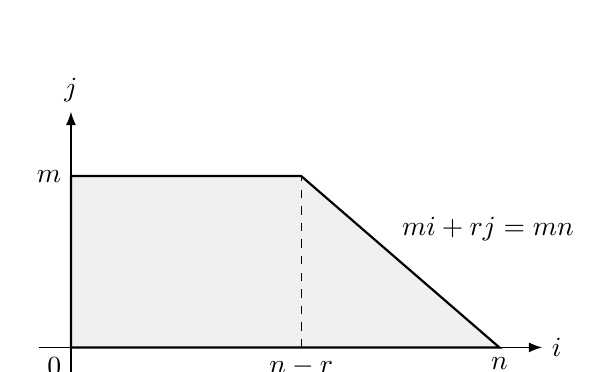
\begin{tikzpicture}[x=0.68cm,y=0.68cm,>=Latex]
\draw[->] (-0.6,0)--(8.8,0) node[right] {$i$};
\draw[->] (0,-0.6)--(0,4.4) node[above] {$j$};
\fill[black!6] (0,0)--(8,0)--(4.3,3.2)--(0,3.2)--cycle;
\draw[thick] (0,0)--(8,0)--(4.3,3.2)--(0,3.2)--cycle;
\node[below left] at (0,0) {$0$};
\node[below] at (8,0) {$n$};
\node[left] at (0,3.2) {$m$};
\draw[dashed] (4.3,0)--(4.3,3.2);
\node[below] at (4.3,0) {$n-r$};
\node[above right] at (6.0,1.8) {$mi+rj=mn$};
\end{tikzpicture}
\caption{The prescribed support. The slope parameter $r$ records how far the
upper right corner is removed. The picture is schematic.}
\label{n:fig:polygon}
\end{figure}

The upper bound records this sloping edge, rather than only the enclosing
rectangle. Put $g=\gcd(m,r)$.
\begin{thm}\label{n:thm:polygon}
For $f\in\Tcal_{m,n,r}$ the zero set of $F$ is finite and
\begin{equation}\label{n:eq:upper}
 N(F)\le\min\{n^2,\ (4m+1)n-m^2-4m-(m-1)r-g\}.
\end{equation}
\end{thm}

One endpoint of Figure~\ref{n:fig:polygon} is particularly useful. Let
$\Ecal_{m,n}$ be the entire coefficient space
\begin{equation}\label{n:eq:Eclass}
 F(z)=c z^n+
 \sum_{\substack{i,j\ge0,\ i+j\le n-1\\j\le m}}c_{ij}z^i\bar z^j,
 \qquad c\ne0.
\end{equation}
The only restriction on its top homogeneous part is that it be holomorphic;
the lower terms are neither real-valued nor harmonic in general. Denote its
largest zero count by $E_{m,n}$. This is a finite integer by
Theorem~\ref{n:thm:polygon}.

The asymptotic coefficient in this full space is sharp.
\begin{thm}\label{n:thm:E}
For $n>m\ge1$,
\begin{equation}\label{n:eq:Eupper}
 E_{m,n}\le\min\{n^2,\ (4m+1)n-2m(m+2)\}.
\end{equation}
For $n>4m+1$,
\begin{equation}\label{n:eq:Elower}
 E_{m,n}\ge(4m+1)n-4m(2m+1).
\end{equation}
The lower bound is attained by a polynomial all of whose zeros are
nondegenerate. For every fixed $m$,
\begin{equation}\label{n:eq:limit}
 \lim_{n\to\infty}\frac{E_{m,n}}n=4m+1.
\end{equation}
\end{thm}

Indeed, the lattice condition in \eqref{n:eq:support} with $r=m+1$ is exactly
\eqref{n:eq:Eclass}. For $1\le j\le m$ it is equivalent to $i+j\le n-1$;
for $j=0$ it is $i\le n$. This proves \eqref{n:eq:Eupper} from
\eqref{n:eq:upper}. The construction proving \eqref{n:eq:Elower} is given in
Section~\ref{n:sec:construction}. The optimized lower bound in Theorem~\ref{new:thm:pure} improves \eqref{n:eq:Elower} in a finite-degree range, and \eqref{new:eq:uniformpure} gives an all-degree error estimate. The gap between the two older linear expressions
is $6m^2$. Thus \eqref{n:eq:limit} does not assert equality in
\eqref{n:eq:Eupper} for each pair $(m,n)$.

The other endpoint includes the total-degree class studied by S\`ete and Zur
\cite[Section~5]{SZ24}. It is substantially smaller than \eqref{n:eq:Eclass}.
\begin{cor}\label{n:cor:total}
If $\deg p=n>m\ge1$ and $\deg_{\rm tot}Q\le m$, then
\begin{equation}\label{n:eq:total}
 \#\{z:p(z)+Q(z,\bar z)=0\}
 \le\min\{n^2,\ (3m+2)n-m^2-4m-\gcd(m,n)\}.
\end{equation}
\end{cor}
\begin{proof}
Every mixed monomial in $Q$ satisfies
$mi+nj\le n(i+j)\le nm$. All analytic terms of $p$ also satisfy this
inequality. Apply Theorem~\ref{n:thm:polygon} with $r=n$.
\end{proof}

In particular, the second estimate in \eqref{n:eq:total} is not restricted to
harmonic polynomials. This extension does not identify the maximum in the
total-degree class with the harmonic maximum. Nor does the asymptotic result
\eqref{n:eq:limit} apply to that smaller class: the allowed mixed terms in
\eqref{n:eq:Eclass} can have degrees tending to $n$.

For comparison with prior work, the case of conjugate degree one is a
rational harmonic equation. Its sharper degree-dependent bounds are due to
Liesen and Zur \cite[Theorem~1.1, author version v2, p.~2]{LZ18}; sharpness
with prescribed pole multiplicities follows from Lee and Makarov
\cite[Theorem~C, p.~3]{LM14}. We record this known endpoint in
Section~\ref{n:sec:known}, rather than count it as a new result.

\subsection{Genericity within the support restriction}\label{n:sec:reg}
The inequality $r>m$ makes $cz^n$ the unique highest-total-degree term.
Lemma~\ref{d:lem:pure}, after scaling, gives finiteness and $N(F)\le n^2$.
The support in \eqref{n:eq:support} is downward closed, so
Corollary~\ref{core:regularizationspace} applies without enlarging it.
Thus we may preserve all zeros through regularization and then make a
small generic perturbation in the same support.

A sufficiently small further perturbation preserves any finite set of
nondegenerate zeros. We may consequently assume that the affine curve
$C=\{f=0\}$ is smooth and irreducible, that its finite intersections with
$\tau C$ are transverse, and that $C$ is transverse to the fixed set of
\[
 \tau(z,w)=(\bar w,\bar z).
\]
These are genuine generic conditions in the indicated sparse space.
The monomials $1,z,w$ separate first-order jets at affine points and
separate two different affine points. They give the required transversality
both off and on the fixed set. Irreducibility is a nonempty algebraic open
condition: $w^m+z^n+z$ belongs to the space and is irreducible by Eisenstein
at $z$ (the case $m=1$ is immediate). We may also assume the leading
coefficient in $w$ has simple zeros, the next coefficient is nonzero there,
and the polynomial on the sloping Newton edge has distinct nonzero roots.
These are compatible open conditions. All subsequent arguments concern
such a perturbation.

\subsection{The normalization genus}\label{n:sec:genus}
Write
\[
 f(z,w)=\sum_{j=0}^m a_j(z)w^j,
 \qquad \deg a_j\le\left\lfloor n-\frac{rj}{m}\right\rfloor.
\]
Let $\widetilde C$ be the normalization of the closure of $C$ in
$X=\CP^1_z\times\CP^1_w$, and let $\gamma$ be its genus. The projection
$z:\widetilde C\to\CP^1$ has degree $m$.

The genus can be bounded directly from the discriminant; no nonsingularity
of the curve at infinity is being assumed. Lemma~\ref{n:lem:genus} provides the
precise estimate used in the surface argument.
\begin{lem}\label{n:lem:genus}
For the generic curve just described,
\begin{equation}\label{n:eq:genus}
 2\gamma\le(2m-2)n-(m-1)r-m-g+2.
\end{equation}
Above $(\infty,\infty)$ there are exactly $g$ points of the normalization,
with local parametrizations
\begin{equation}\label{n:eq:branches}
 u=t^{m/g},\qquad v=c_\ell t^{r/g}(1+O(t)),\qquad c_\ell\ne0,
 \quad u=1/z,\ v=1/w.
\end{equation}
\end{lem}
\begin{proof}
The discriminant $\Disc_w f$ is homogeneous of degree $2m-2$ in the
coefficients $a_j$, and homogeneous of weight $m(m-1)$ when $a_j$ has
weight $j$. Therefore
\[
 \deg_z\Disc_w f\le (2m-2)n-r(m-1).
\]
When $m=1$, the discriminant is $1$ and this bound is zero.
Over a finite value of $z$ with $a_m\ne0$, its order is the total
ramification multiplicity, because the affine curve is smooth. At a zero
of $a_m$, the branch at $w=\infty$ is unramified: in $v=1/w$ the equation
is $a_m(z)+a_{m-1}(z)v+O(v^2)=0$, and both $a_m'(z)$ and $a_{m-1}(z)$
are nonzero there. The other branches are generically unramified there
as well. Thus the finite ramification contribution is at most
$(2m-2)n-r(m-1)$.

Near $(\infty,\infty)$, multiply $f(1/u,1/v)$ by $u^nv^m$.
Put $a=m/g$, $b=r/g$. Its terms of least $(a,b)$-weight form
\[
 c\prod_{\ell=1}^g(v^a-\lambda_\ell u^b),
 \qquad c\ne0,
\]
where the $\lambda_\ell$ are distinct and nonzero. All other terms have
strictly larger weight. Substituting $u=t^a$, $v=t^bV$ and dividing by the
least power of $t$ gives a polynomial in $V$ with $m$ simple nonzero roots
at $t=0$. The holomorphic implicit function theorem gives the local
expansions. Grouping the roots by the action $t\mapsto e^{2\pi i/a}t$
yields exactly $g$ branches and gives \eqref{n:eq:branches}.
There are no other points above $z=\infty$. Their total ramification is
$g(a-1)=m-g$.

Riemann--Hurwitz now gives
\[
 2\gamma-2\le-2m+(2m-2)n-r(m-1)+(m-g),
\]
which is \eqref{n:eq:genus}.
\end{proof}

The right side of \eqref{n:eq:genus} is twice the number of interior lattice
points in Figure~\ref{n:fig:polygon}. Only the displayed genus inequality is needed here.

\subsection{The quotient surface and its end}\label{n:sec:surface}
The symmetric-product map
\[
 \Phi:X\longrightarrow\operatorname{Sym}^2(\CP^1)=\CP^2,
 \qquad \Phi(z,w)=\{z,\bar w\},
\]
has fibers equal to the $\tau$-orbits. In affine coordinates it is
$[1:z+\bar w:z\bar w]$. Its restriction to the smooth affine curve is an
immersion. To check this at a fixed point, use real coordinates
$s=(z+\bar w)/2$, $t=(z-\bar w)/2$. The quotient has local form
$(s,t)\mapsto(s,t^2)$ and kernel $J(T\Fix(\tau))$. A complex tangent line
transverse to $T\Fix(\tau)$ is also transverse to its $J$-image. Away from
the fixed set the quotient is a local diffeomorphism.

The ordinary projective closures of $f=0$ and $f^*=0$ have no common point
at infinity and have degrees $n,n$. In generic position they therefore
have $n^2$ distinct affine intersections. Of these, $N(F)$ are fixed and
the rest occur in pairs. The affine image has
\begin{equation}\label{n:eq:D}
 D_+=\frac{n^2-N(F)}2
\end{equation}
ordinary double points. They are positive: the intersection of the two
complex curves is positive, transport of the second sheet by the
anti-holomorphic involution reverses its two-dimensional orientation, and
$\Phi$ reverses the ambient four-dimensional orientation. The two changes
cancel. There are no triple points, since fibers have size at most two.

If $\alpha,\beta$ are the positive cohomology generators of the two factors
and $H$ is the hyperplane class, then $\Phi^*H=\alpha-\beta$. The coordinate
projections on $\widetilde C$ have degrees $m,n$. Thus the image homology
class has degree $m-n$. Reversing the source orientation makes it positive,
of degree $d=n-m$. This reversal does not change double-point signs.

The finite points of $C$ on $w=\infty$ are smooth, unramified points with
distinct images. Their partners under $\tau$ are not on $C$, since $C$
has no point with $z=\infty,w\ne\infty$. They introduce no additional
double points. It remains to treat $(\infty,\infty)$.

The required filling is elementary at the level of parametrized complex
curves. We spell out why its double points have the correct sign.
\begin{lem}\label{n:lem:cap}
The mirror torus link $T(a,-b)$, with $a,b>0$, bounds
$\gcd(a,b)$ immersed oriented disks in a four-ball, with only negative
ordinary double points.
\end{lem}
\begin{proof}
The normalization of the complex curve $Y^a=X^b$ in a small ball is a
union of $e=\gcd(a,b)$ disks, parametrized by
$(X,Y)=(t^{a/e},\zeta_\ell t^{b/e})$. Perturb these parametrizations by
sufficiently small holomorphic polynomial maps. Generic such perturbations
have nonzero derivative, only transverse double intersections, and no
triple intersections. This follows from jet transversality: polynomial
variations of sufficiently large degree interpolate the first jets at one
point and the values at two or three distinct points. The respective bad
conditions have the required real codimensions $4,4,8$.
All transverse intersections are positive because the disks are complex
curves. Near the boundary the unperturbed maps are embedded and transverse
to the sphere; their perturbed inverse images of the ball remain disks and
the boundary link remains isotopic to $T(a,b)$.
Reflect one complex coordinate of the ambient ball. It reverses its
orientation, turns every double point negative, and mirrors the boundary
link. A collar realizing the boundary isotopy gives the claimed filling.
\end{proof}

We next identify the actual link, including a Newton edge with more than two
monomials. Put $a=m/g$, $b=r/g$, so $b>a$. Near $\Phi(\infty,\infty)$
use coordinates
\[
 X=u+\bar v,\qquad Y=u\bar v.
\]
By \eqref{n:eq:branches}, $|v|=o(|u|)$ and $X=u(1+o(1))$.
For the branch associated with $\lambda_\ell$ the boundary on $|X|=\rho$
satisfies, after $Y=\rho^{1+b/a}\eta$,
\begin{equation}\label{n:eq:braid}
 \eta^a=\overline{\lambda_\ell}e^{-i(b-a)\theta}+o(1),
 \qquad X=\rho e^{i\theta}.
\end{equation}
The convergence is in $C^1$ in the angular parametrizations. The roots of
the limiting equations are distinct and nonzero, so the small error in
\eqref{n:eq:braid} does not alter the braid type.

Move the $g$ distinct nonzero constants $\overline{\lambda_\ell}$ through
a path of distinct nonzero configurations to a scaled set of $g$th roots
of unity. The displayed roots never collide, so this gives a link isotopy.
The resulting union is
\[
 \eta^m=C e^{-i(r-m)\theta},\qquad C\ne0,
\]
which is $T(m,-(r-m))$. It has $\gcd(m,r-m)=g$ components, in agreement
with the $g$ normalization disks. A rounded bidisk in the $(X,Y)$ chart
is a four-ball whose boundary contains this braid; by taking $\rho$ small,
the curve meets its boundary only on this part. Formula
\eqref{n:eq:branches} also shows that its inverse image consists of $g$
disks. Their induced orientations agree with the complex-parameter
orientations of the mirrored torus link. If the whole source is reversed,
reverse the orientations of all filling disks as well.

Replace these disks by the fillings in Lemma~\ref{n:lem:cap}, matching collars
by the link isotopy. No source handle is introduced, all new double points
are negative, and a replacement inside a ball does not change the global
homology class. We obtain a closed connected immersed surface of genus
$\gamma$, degree $d=n-m$, and exactly the positive double points in
\eqref{n:eq:D}.

We use the immersed Thom inequality in the following precise form:
\begin{equation}\label{n:eq:thom}
 \gamma+D_+\ge\frac{(d-1)(d-2)}2.
\end{equation}
The version allowing only negative double points is stated in Orevkov
\cite[Theorem~3.1, author version v2, p.~8]{Ore24}, with attribution to
Kronheimer--Mrowka \cite{KM94}. Resolving each positive double point by an
oriented annulus increases the genus by one, leaves the homology class
unchanged, and reduces the general case to that version. Thus it is
\eqref{n:eq:thom}, not an inequality for a singular image, that applies.

Combining \eqref{n:eq:genus}, \eqref{n:eq:D}, and \eqref{n:eq:thom} yields
\[
 N(F)\le n^2+(2m-2)n-(m-1)r-m-g+2
       -(n-m-1)(n-m-2).
\]
The expression simplifies to the second bound in \eqref{n:eq:upper}.
Lemma~\ref{core:regularizationspace} and the preservation of nondegenerate zeros under the
subsequent small perturbation transfer it to every initial polynomial.
This proves Theorem~\ref{n:thm:polygon}.

\subsection{An exact count of zeros approaching infinity}\label{n:sec:infinity}
Adding a higher analytic monomial changes both the leading homogeneous part
and the degree at infinity. In the following situation every added zero
can be counted, without an uncontrolled intermediate scale.
\begin{lem}\label{n:lem:infinity}
Let $k>m\ge1$, $r>m$, and let $P\in\C[z,w]$ have degrees at most $k,m$
in $z,w$, respectively, with $[z^kw^m]P=c\ne0$. Suppose all zeros of
$P(z,\bar z)$ are nondegenerate. For all sufficiently small real
$\varepsilon>0$, the polynomial
\[
 F_\varepsilon(z)=P(z,\bar z)+\varepsilon z^{k+r}
\]
has exactly $N(P(z,\bar z))+r+m$ zeros, all nondegenerate. The $r+m$ new
zeros approach infinity and have positive Jacobian.
\end{lem}
\begin{proof}
The term $cz^kw^m$ is the unique term of total degree $k+m$. All old zeros
are confined to a compact set, and each persists uniquely under the small
perturbation. Set $t=\varepsilon^{1/(r-m)}$ and $z=\zeta/t$. On compact
$\zeta$-sets,
\begin{equation}\label{n:eq:scaling}
 t^{k+m}F_\varepsilon(\zeta/t)
 =\zeta^k(\zeta^r+c\bar\zeta^m)+O(t),
\end{equation}
with $C^1$ convergence. The nonzero zeros of the limit satisfy
\[
 |\zeta|^{r-m}=|c|,
 \qquad (r+m)\arg\zeta=\arg(-c)\pmod{2\pi}.
\]
There are exactly $r+m$. At such a zero the Jacobian of
$\zeta^r+c\bar\zeta^m$ is
\[
 (r^2-m^2)|\zeta|^{2r-2}>0.
\]
Multiplication by $\zeta^k$ preserves its sign. The implicit function theorem
applied to \eqref{n:eq:scaling} gives one simple positive zero near each.

For completeness, choose $R$ so large that
\[
 |P(z,\bar z)-cz^k\bar z^m|
 \le \tfrac12|c|\,|z|^{k+m}\quad (|z|\ge R).
\]
Any zero of $F_\varepsilon$ there must satisfy
\[
 \tfrac12|c|\le \varepsilon|z|^{r-m}\le\tfrac32|c|.
\]
Its scaled coordinate $\zeta=tz$ therefore lies in a fixed compact annulus.
Every limit point in that annulus is one of the above $r+m$ simple zeros;
compactness and local uniqueness exclude further zeros there.
On $|z|\le R$, compactness away from disjoint old-zero neighborhoods excludes
all other zeros for small $\varepsilon$. This proves the exact count.
\end{proof}

The lemma applies to the full rectangle of exponents $i\le k,j\le m$.
After adding $z^{k+r}$, this rectangle and the new exponent all belong to
\eqref{n:eq:support} with $n=k+r$, because $mi+rj\le mk+rm=mn$.


\subsection{The optimal coefficient in the support-restricted space}\label{n:sec:construction}
The radial polynomial in Proposition~\ref{b:prop:radial}, with analytic
degree $k>3m$, has $(4m+1)(k-m)$ nondegenerate zeros and a nonzero
coefficient at $z^kw^m$. Its coefficients may be chosen real rational.
We combine it with the preceding exact count at infinity.

Denote the largest zero count in $\Tcal_{m,n,r}$ by $K_{m,n,r}$.
The combination of the preceding lemmas proves a slightly more general
asymptotic statement than Theorem~\ref{n:thm:E}.
\begin{prop}\label{n:prop:lower}
If $n>r+3m$ and $r>m$, then
\begin{equation}\label{n:eq:Klower}
 K_{m,n,r}\ge(4m+1)n-4m(r+m).
\end{equation}
For fixed $m,r$ with $r>m$, $\lim_{n\to\infty}K_{m,n,r}/n=4m+1$.
\end{prop}
\begin{proof}
Put $k=n-r>3m$. Lemma~\ref{b:prop:radial} gives $(4m+1)(k-m)$ zeros.
Lemma~\ref{n:lem:infinity} adds exactly $r+m$, giving
\[
 (4m+1)(n-r-m)+(r+m)=(4m+1)n-4m(r+m).
\]
The resulting polynomial lies in $\Tcal_{m,n,r}$ by the observation at the
end of Section~\ref{n:sec:infinity}. This proves \eqref{n:eq:Klower}; dividing
it and \eqref{n:eq:upper} by $n$ proves the limit.
\end{proof}

For $r=m+1$ this gives \eqref{n:eq:Elower}. Together with
\eqref{n:eq:Eupper}, it proves \eqref{n:eq:limit} and completes
Theorem~\ref{n:thm:E}. All constructed zeros are nondegenerate, and the final
$\varepsilon$ can be chosen positive rational.

The distinction between the two support restrictions is substantive.
For example, when $m\ge2$ is fixed, Corollary~\ref{n:cor:total} bounds the
leading coefficient for $p+Q$ with $\deg_{\rm tot}Q\le m$ by $3m+2$,
whereas Theorem~\ref{n:thm:E} gives the strictly larger optimal coefficient
$4m+1$ in \eqref{n:eq:Eclass}. Both classes have holomorphic highest
homogeneous term. That condition alone is therefore insufficient to
obtain the lower coefficient.

\subsection{A known sharp endpoint and the remaining gap}\label{n:sec:known}
There is a complete degree-dependent answer when $m=1$. We include it to
locate the new bounds relative to established sharp results.
\begin{prop}\label{n:prop:known}
For $2\le r\le n$,
\begin{equation}\label{n:eq:known}
 K_{1,n,r}=5n-2r-2.
\end{equation}
In particular, $E_{1,n}=5n-6$ for every $n\ge2$.
\end{prop}
\begin{proof}
Write $f=p(z)-wq(z)$, with $\deg p=n$, $\deg q\le n-r$.
If $q\equiv0$, the elementary analytic bound suffices. Otherwise, remove
a greatest common divisor of degree $s$, leaving numerator and denominator
degrees $a=n-s$ and $b\le n-r-s$. The rational harmonic bound in
\cite[Theorem~1.1, author version v2, p.~2]{LZ18} gives
\[
 N(f(z,\bar z))\le s+3a+2b-2\le5n-2r-2.
\]
Here $a-b\ge r\ge2$; denominator zeros are not rational zeros because the
reduced pair is coprime.

For equality, apply Lee--Makarov's Theorem~C
\cite[p.~3]{LM14} with rational degree $n$, one pole of order $r$ at
infinity, and $n-r$ simple finite poles. There are $n-r+1$ distinct poles.
Their theorem gives
\[
 \min\{3n+2(n-r+1)-3,5n-5\}=5n-2r-1
\]
fixed points on the sphere. Infinity is one, leaving $5n-2r-2$ finite
zeros. The numerator and denominator degrees are $n,n-r$.
Regularity of an extremizer also follows from
\cite[Theorem~3.5, author version v2, p.~7]{LZ18}.
Taking $r=2$ proves the last assertion.
\end{proof}

Proposition~\ref{n:prop:known} is already implicit in those results and is not
claimed here as new. It also shows that the upper bound in
Theorem~\ref{n:thm:polygon} is not always the finite-degree maximum: for
$m=1,r>2$ it gives $5n-6$, whereas \eqref{n:eq:known} is smaller.

The finite-degree equalities proved later in Theorem~\ref{d:thm:main}
settle part of this range. The general expression in
Theorem~\ref{n:thm:polygon} is an upper bound, not a claim of equality
for every triple $(m,n,r)$.

\section{A bound depending on the total-degree gap}\label{g:sec:gap}
Let $1\le m<n$, let $p\in\C[z]$ have degree $n$, and let
$Q\in\C[z,w]$ have total degree at most $m$. We write
\begin{equation}\label{g:eq:F}
 F(z)=p(z)+Q(z,\bar z),\qquad d=n-m,\qquad
 N(F)=\#\{z\in\C:F(z)=0\}.
\end{equation}
In this note the first variable of $Q$ is the analytic variable. The
restriction on $Q$ is a \emph{total-degree} restriction, not merely a bound
on its degree in $w$. Thus the class in \eqref{g:eq:F} contains every harmonic
polynomial $p+\overline q$ with $\deg q\le m$, but it does not contain all
polyanalytic polynomials of bidegree $(m,n)$.

The classical harmonic estimate is $n^2$; see Wilmshurst
\cite[pp.~2077--2079]{Wil98}. The Hermitian trace approach developed by
Furch\`i gives $n^2-2$ when $m\le n-2$, subject in his statement to a possible
$n^2-1$ exception determined by two analytic coefficients
\cite[Theorem~1.1, author version v2, p.~2]{Fur25}.
The proof below removes that exception and permits mixed lower-degree terms. The estimate below takes account of
the entire gap between the two degrees.

This is the main result of the present note.
\begin{thm}\label{g:thm:main}
Under the assumptions in \eqref{g:eq:F}, the zero set of $F$ is finite and
\begin{equation}\label{g:eq:bound}
 N(F)\le n^2-2\left\lfloor\frac{(n-m)^2}{4}\right\rfloor.
\end{equation}
\end{thm}

For $d=2$, \eqref{g:eq:bound} is $n^2-2$. For $d=3,4,5,6$ the deficits from
$n^2$ become $4,8,12,18$, respectively. For large $n$ with $m$ fixed, this is
still a quadratic estimate; it is not a replacement for the linear bound
of Corollary~\ref{n:cor:total}. Rather, the two bounds are effective in different regimes.
No claim of sharpness for every $d$ is made.

The proof uses the standard Hermitian trace form, whose signature counts
real solutions in the appropriate real structure. That correspondence is
Furch\`i's Theorem~3.13 and Corollary~3.14
\cite[author version v2, pp.~9--10]{Fur25}; we include the required argument,
including multiple complex roots. The additional ingredient is a totally
isotropic subspace of dimension $\lfloor d^2/4\rfloor$. 
\subsection{The quotient algebra and its Hermitian form}
Divide $F$ by the leading coefficient of $p$, so that $p$ is monic.
For a univariate polynomial $a$, put
$a^\#(w)=\overline{a(\bar w)}$. For $a\in\C[z,w]$, put
\[
 a^*(z,w)=\overline{a(\bar w,\bar z)}.
\]
The latter is a conjugate-linear involution. Define
\begin{equation}\label{g:eq:algebra}
 f=p(z)+Q(z,w),\qquad
 f^*=p^\#(w)+Q^*(z,w),\qquad
 \A=\C[z,w]/(f,f^*).
\end{equation}
With any graded monomial order, the leading monomials of $f$ and $f^*$ are
$z^n$ and $w^n$. Since these are relatively prime, the two polynomials form
a Gr\"obner basis. Consequently
\begin{equation}\label{g:eq:basis}
 \{z^i w^j:0\le i,j<n\}
\end{equation}
is a basis of $\A$ and $\dim_\C\A=n^2$. This proves, in particular, the
finiteness assertion in Theorem~\ref{g:thm:main}. We identify a polynomial
with its class when no ambiguity can arise.

For $a\in\A$, let $M_a$ denote multiplication by $a$, and set
\begin{equation}\label{g:eq:form}
 T(a)=\Tr M_a,\qquad \HH(a,b)=T(ab^*).
\end{equation}
The ideal in \eqref{g:eq:algebra} is invariant under $*$, so these expressions
are well defined. Moreover $T(a^*)=\overline{T(a)}$; hence $\HH$ is Hermitian.
The involution satisfies
$\HH(a^*,b^*)=\overline{\HH(a,b)}$.

The signature is the positive index minus the negative index; the radical
is the nullspace. The following form of the signature theorem retains
all multiplicities throughout the algebraic argument.
\begin{lem}\label{g:lem:signature}
The signature of $\HH$ is $N(F)$. If $R$ is the number of distinct common
zeros of $f,f^*$ and $s$ is the number of two-element orbits of
$(z,w)\mapsto(\bar w,\bar z)$ on this set, then
\[
 \rank\HH=R,\qquad \nu_-(\HH)=s,\qquad
 N(F)=R-2s.
\]
Here $\nu_-$ denotes the number of negative eigenvalues, counted with
multiplicity.
\end{lem}
\begin{proof}
Decompose the finite algebra into its local algebras. On a local algebra
of length $\mu$ supported at $x$, multiplication by $a$ has trace
$\mu a(x)$: the difference from scalar multiplication is nilpotent.
At a fixed point of the involution the resulting trace form has a single
positive eigenvalue, with coefficient $\mu$, and is zero on the maximal
ideal. At a nonfixed pair $x,x^*$, the two local lengths agree; on their
constant coordinates the matrix of the form is
\[
 \begin{pmatrix}0&\mu\\ \mu&0\end{pmatrix}.
\]
It has one positive and one negative eigenvalue. The remaining local
coordinates are in the radical. Different orbits are orthogonal. Adding
these contributions proves the assertions and identifies the fixed
points with the zeros of $F$.
\end{proof}

A single isotropic subspace can lose dimension in the radical. The
involution provides precisely the control needed to handle this loss.
\begin{lem}\label{g:lem:isotropic}
Let $V$ be a finite-dimensional complex vector space with a Hermitian form
$H$ and a conjugate-linear involution $J$ satisfying
$H(Ju,Jv)=\overline{H(u,v)}$. If $U\subset V$ is totally isotropic and
$U\cap JU=\{0\}$, then
\begin{equation}\label{g:eq:signaturebound}
 \operatorname{signature}H\le \dim V-2\dim U.
\end{equation}
\end{lem}
\begin{proof}
Put $r=\dim\rad H$ and $k=\dim(U\cap\rad H)$. The radical is $J$-invariant.
The subspaces $U\cap\rad H$ and $J(U\cap\rad H)$ are disjoint, so $r\ge2k$.
In the nondegenerate quotient $V/\rad H$, the image of $U$ is isotropic of
dimension $\dim U-k$. Projection onto the negative eigenspace is injective
on any isotropic subspace of a nondegenerate Hermitian space. Therefore
$\nu_-(H)\ge\dim U-k$. It follows that
\[
 \operatorname{signature}H
 =\dim V-r-2\nu_-(H)
 \le\dim V-2\dim U-r+2k
 \le\dim V-2\dim U,
\]
as required.
\end{proof}

We shall apply \eqref{g:eq:signaturebound} to \eqref{g:eq:form}. No simplicity
assumption on the roots of the complexified system will be needed.

\subsection{An exact trace identity below degree \texorpdfstring{$2d$}{2d}}
Write
\[
 Q(z,w)=\sum_{r+s\le m}c_{rs}z^rw^s.
\]
For a univariate polynomial $u$, let
\[
 S(u)=\Tr_{\C[z]/(p)} M_u,
 \qquad
 D_r(u)=[z^{n-1}]\bigl(z^ru'(z)\bmod p(z)\bigr).
\]
The remainder in this definition has degree less than $n$. Use
$S^\#,D_r^\#$ for the corresponding functionals defined by $p^\#$ in the
variable $w$. These are complex-linear functionals. In particular,
\begin{equation}\label{g:eq:Dvanish}
 D_r(u)=0\quad\hbox{if }\deg u+r<n,
\end{equation}
and the same assertion holds for $D_r^\#$. Also
$S^\#(u^\#)=\overline{S(u)}$.

The next identity, rather than just a single vanishing trace, is the
algebraic input to the proof.
\begin{lem}\label{g:lem:traceidentity}
If $u\in\C[z]$, $v\in\C[w]$, and $\deg u+\deg v<2d$, then
\begin{equation}\label{g:eq:traceidentity}
\begin{split}
 T(u(z)v(w))={}&S(u)S^\#(v)\\
 &-\sum_{r+s\le m}c_{rs}D_r(u)S^\#(w^s v)\\
 &-\sum_{r+s\le m}\bar c_{rs}S(z^s u)D_r^\#(v).
\end{split}
\end{equation}
\end{lem}
\begin{proof}
Introduce a real parameter $t$ and replace $Q,Q^*$ by $tQ,tQ^*$ in
\eqref{g:eq:algebra}; denote the multiplication trace by $T_t$. The standard
basis \eqref{g:eq:basis} is unchanged for every $t$.

We first show that $T_t(z^a w^b)$ is affine in $t$ when $a+b<2d$.
To compute a diagonal entry of the multiplication matrix, reduce
$z^{a+i}w^{b+j}$ to standard monomials. A substitution using a lower term
of $p$ or $p^\#$ decreases total degree by at least one. A substitution
using a term of $tQ$ or $tQ^*$ decreases total degree by at least $n-m=d$
and contributes one factor of $t$. A reduction path ending in $z^iw^j$
can decrease degree by only $a+b$. It therefore uses at most one term
containing $t$. All reductions strictly decrease total degree, so they
terminate, and each diagonal entry is affine in $t$. Linearity gives the
same assertion for $T_t(uv)$.

Suppose first that $p$ has distinct roots $\alpha_1,\ldots,\alpha_n$.
At $t=0$, the roots of the complexified system are the simple grid points
$(\alpha_a,\bar\alpha_b)$. Their derivatives satisfy
\[
 z'_{ab}(0)=-\frac{Q(\alpha_a,\bar\alpha_b)}{p'(\alpha_a)},\qquad
 w'_{ab}(0)=-\frac{Q^*(\alpha_a,\bar\alpha_b)}{(p^\#)'(\bar\alpha_b)}.
\]
For small $t$, the trace is the sum of the values of $uv$ at these
$n^2$ simple roots. Differentiating this sum at zero gives
\eqref{g:eq:traceidentity}, because Lagrange interpolation yields
\begin{equation}\label{g:eq:lagrange}
 D_r(u)=\sum_{a=1}^n
 \frac{\alpha_a^r u'(\alpha_a)}{p'(\alpha_a)}.
\end{equation}
Indeed, the right side is the coefficient of $z^{n-1}$ in the remainder of
$z^ru'$ modulo $p$. The constant term in $t$ is $S(u)S^\#(v)$, and the two
sums in \eqref{g:eq:traceidentity} are its first derivative. Affineness in $t$
makes this first-order identity exact at $t=1$.

Finally, all expressions in \eqref{g:eq:traceidentity}, with $D_r$ defined by
remainders, are polynomial functions of the coefficients of $p,Q$ and
their conjugates. The identity therefore extends from polynomials $p$ with
simple roots to all monic $p$. Formula~\eqref{g:eq:lagrange} is used only in
the proof on the dense simple-root locus.
\end{proof}

The threshold $2d$ is important. At total degree $2d$, two substitutions
using the perturbation can contribute to a diagonal entry, and the trace
need not be affine in $Q$. We do not use \eqref{g:eq:traceidentity} at that
threshold or beyond it.

\subsection{A large isotropic subspace}
For the moment assume that the leading moment matrices
\begin{equation}\label{g:eq:momentcondition}
 \bigl(S(z^{a+b})\bigr)_{0\le a,b\le k},\qquad 0\le k<d,
\end{equation}
are nonsingular. This is a nonempty Zariski-open condition on the
coefficients of $p$. To see nonemptiness, take $p$ with $n$ distinct real
roots: the matrices are positive definite for $k<n$, by evaluation of a
nonzero real polynomial of degree at most $k$ at those roots.

Apply Gram--Schmidt to $1,z,\ldots,z^{d-1}$ for the complex bilinear pairing
$(a,b)\mapsto S(ab)$. The result is a sequence of monic polynomials
$r_i$ of degree $i$, satisfying
\begin{equation}\label{g:eq:orthogonality}
 S(r_i a)=0\quad(\deg a<i),\qquad 0\le i<d.
\end{equation}
This is bilinear orthogonality, not Hermitian orthogonality. Positivity is
not assumed for the general complex polynomial $p$.

We can now construct the subspace needed in Lemma~\ref{g:lem:isotropic}.
\begin{prop}\label{g:prop:U}
Under \eqref{g:eq:momentcondition}, the subspace
\begin{equation}\label{g:eq:U}
 U=\spanC\{r_i(z)r_j^\#(w):0\le j<i,\ i+j\le d-1\}\subset\A
\end{equation}
is totally isotropic for $\HH$, satisfies $U\cap U^*=\{0\}$, and has
complex dimension $\lfloor d^2/4\rfloor$.
\end{prop}
\begin{proof}
The products $r_i(z)r_j^\#(w)$ with $0\le i,j<d$ are linearly independent
in \eqref{g:eq:basis}. The involution exchanges their two indices.
The index sets defining $U$ and $U^*$ are disjoint, which proves
$U\cap U^*=\{0\}$. Counting the pairs with $i>j$ and $i+j\le d-1$ gives
\begin{equation}\label{g:eq:dimension}
 \dim U=
 \begin{cases}
 t^2,&d=2t,\\
 t(t+1),&d=2t+1,
 \end{cases}
 =\lfloor d^2/4\rfloor.
\end{equation}

Take indices $(i,j),(k,\ell)$ occurring in \eqref{g:eq:U} and put
\[
 u=r_i r_\ell,\qquad v=r_j^\# r_k^\#.
\]
Their total degree is at most $2d-2$, so Lemma~\ref{g:lem:traceidentity}
applies. The constant term $S(r_i r_\ell)S^\#(r_j^\#r_k^\#)$ is zero:
by \eqref{g:eq:orthogonality}, both factors could be nonzero only if
$i=\ell$ and $j=k$, contradicting $i>j$ and $k>\ell$.

Consider a term with coefficient $c_{rs}$ in the first sum of
\eqref{g:eq:traceidentity}. If $D_r(u)\ne0$, then \eqref{g:eq:Dvanish} implies
$i+\ell+r\ge n$. Since $i+j\le n-m-1$, it follows that
\[
 \ell-j\ge m+1-r,\qquad k-j\ge m+2-r>s.
\]
Thus $j+s<k$, and \eqref{g:eq:orthogonality} implies
$S^\#(w^s r_j^\# r_k^\#)=0$. If $D_r(u)=0$, the same term is zero directly.
Hence every term in the first sum vanishes.

For the second sum, a nonzero $D_r^\#(v)$ would imply $j+k+r\ge n$.
Using $k+\ell\le n-m-1$ and $i>j$, we obtain
\[
 j-\ell\ge m+1-r,\qquad i-\ell\ge m+2-r>s.
\]
Now $\ell+s<i$, so $S(z^s r_i r_\ell)=0$. Every term in the second sum
also vanishes. By \eqref{g:eq:form}, the resulting identity $T(uv)=0$ is
precisely the required pairwise isotropy of $U$.
\end{proof}

Combining Lemmas~\ref{g:lem:signature} and~\ref{g:lem:isotropic} with
Proposition~\ref{g:prop:U}, including \eqref{g:eq:dimension}, proves \eqref{g:eq:bound} under
\eqref{g:eq:momentcondition}. Notice that the common zeros of $f,f^*$ may
have arbitrary multiplicities: the radical estimate in
Lemma~\ref{g:lem:isotropic} has already accounted for them.


\subsection{Removing the auxiliary moment condition}
We finish the proof of Theorem~\ref{g:thm:main}. The coefficient space
$p(z)+Q(z,w)$, $\deg p\le n$, $\deg_{\rm tot}Q\le m$, is stable under
both derivatives. The highest analytic coefficient remains nonzero.
Corollary~\ref{core:regularizationspace} therefore gives an arbitrarily
small perturbation in this space, without decreasing the zero count,
whose zeros are all nondegenerate. A further small change of the
coefficients of $p$ preserves these zeros and satisfies the nonempty
Zariski-open moment condition \eqref{g:eq:momentcondition}. The estimate
proved using Proposition~\ref{g:prop:U} applies to that last polynomial,
and hence to the original one. This proves \eqref{g:eq:bound} with no
assumption on multiplicities or moment matrices.

For a gap of two the bound is $n^2-2$, and it is attained by the
real-valued construction in Theorem~\ref{r:thm:main}, with $m=n-2$.
Consequently the total-degree statement from the earlier drafts is
retained in its strongest form: for $\deg p=n\ge3$ and
$\deg_{\rm tot}Q\le n-2$, the maximum is exactly $n^2-2$.
For larger gaps the formula \eqref{g:eq:bound} is an upper bound,
not an asserted sharp formula. Combining it with
\eqref{n:eq:total} gives the two upper bounds in
Theorem~\ref{core:harmonicbounds} for the harmonic subclass.

\section{Harmonic polynomials with many zeros}\label{b:sec:harmonic}

We now turn to \eqref{b:eq:harmonicfamily}. Unlike the examples in
Section~\ref{b:sec:radial}, every polynomial constructed in this
section is harmonic. The upper bound refines the Descartes argument
of \cite[Section~4.1, \av, pp.~8--9]{Lun23}; the lower bound makes
that argument exact on every line at once. The coefficients on
different lines are not independent, and we keep track of their
common angular dependence throughout.

The full harmonic maximum also equals the maximal valence in that class,
since subtracting a constant preserves both degrees.

Lundberg's probabilistic construction gives
$M^{\mathrm{harm}}_{m,n}\ge\lceil n\sqrt m\rceil$ by using the family
\begin{equation}\label{b:eq:harmonicfamily}
 h(z)=\varepsilon z^n+q(z)+\overline{q(z)},\qquad
 \deg q=m<n,\quad \varepsilon\in\C\setminus\{0\}.
\end{equation}
His concluding question asks for a deterministic choice of $q$ giving
$mn$-order many zeros in this same family
\cite[Section~4.2, \av, p.~9]{Lun23}.
We determine its exact maximal zero count, denoted by $S_{m,n}$.
Put $g=\gcd(m,n)$ and define
\begin{equation}\label{b:eq:harmonicdelta}
 \Delta_{m,n}=
 \begin{cases}
  g,&\text{if $m/g$ and $n/g$ are both odd},\\
  0,&\text{otherwise}.
 \end{cases}
\end{equation}
The correction in \eqref{b:eq:harmonicdelta} comes from the parity of
the exponent gap and a count of equally spaced directions.
\begin{thm}\label{b:thm:harmonic}
For every $1\le m<n$,
\begin{equation}\label{b:eq:harmonicexact}
 S_{m,n}=n(m+1)+\Delta_{m,n}.
\end{equation}
The maximum is attained with $\varepsilon\in\Q_{>0}$ and
$q\in\Q(i)[z]$, and all zeros of the extremizer are nondegenerate.
\end{thm}

\subsection{Real restrictions and the last exponent gap}
For real polynomials the contribution of the final gap can be
bounded more precisely than by two in all cases.
\begin{lem}\label{b:lem:harmonicgap}
Let $N>M\ge0$, let $a\in\R\setminus\{0\}$, and let
$u\in\R[r]$ have degree at most $M$. Write $b=[r^M]u$ for the
coefficient of $r^M$. The number of nonzero real roots of
$ar^N+u(r)$, counted with multiplicity, is at most
\[
 \begin{cases}
  M+1,&N-M\text{ odd},\\
  M+2\mathbf1_{\{ab<0\}},&N-M\text{ even},
 \end{cases}
\]
where the indicator $\mathbf1_{\{ab<0\}}$ equals one when $ab<0$
and zero otherwise.
\end{lem}
\begin{proof}
There is nothing to prove if $u=0$. Otherwise, put $d=\deg u$ and
list its nonzero coefficients in increasing exponent order.
An odd gap between successive exponents contributes exactly one
sign change in total to the coefficient lists of $u(r)$ and
$u(-r)$. An even gap contributes zero or two sign changes, which
is at most its size. The total contribution within $u$ is
therefore at most $d$.

Appending the degree-$N$ coefficient contributes one when $N-d$
is odd. When $N-d$ is even, it contributes two precisely if the
two leading coefficients have opposite signs, and otherwise zero.
If $d=M$, this proves the assertion by Descartes' rule on the two
half-lines. If $d<M$ and $N-M$ is odd, use $d+2\le M+1$.
If $N-M$ is even, the case $d=M-1$ has odd last gap and gives
$d+1=M$; for $d\le M-2$, use $d+2\le M$. These last two cases
also explain why a vanishing coefficient $b$ causes no exception.
\end{proof}

A rotation $z=e^{i\theta}\zeta$ with
$\varepsilon e^{in\theta}>0$ reduces \eqref{b:eq:harmonicfamily} to
$\varepsilon>0$. The transformed polynomial $q(e^{i\theta}\zeta)$
still has degree $m$. After this normalization, the imaginary part
of $h$ vanishes exactly on the lines
\begin{equation}\label{b:eq:harmoniclines}
 \Lambda_j=e^{ij\pi/n}\R,\qquad 0\le j<n.
\end{equation}
Write $q(z)=\sum_{k=0}^m a_kz^k$, with $a_m\ne0$, and put
$\theta_j=j\pi/n$. The restriction to $\Lambda_j$ is the real
polynomial
\begin{equation}\label{b:eq:harmonicrestriction}
 f_j(r)=\varepsilon(-1)^jr^n+
             2\sum_{k=0}^m\Rea(a_ke^{ik\theta_j})r^k.
\end{equation}
Its leading coefficient never vanishes. In particular, every member
of \eqref{b:eq:harmonicfamily} has a finite zero set, and the possible
integer counts are bounded. Thus the maximum defining $S_{m,n}$
exists.

\subsection{The exact upper bound}
Assume first that $\Rea a_0\ne0$. The origin is not a zero, so
counts on the distinct lines \eqref{b:eq:harmoniclines} may be added.
If $n-m$ is odd, Lemma~\ref{b:lem:harmonicgap} gives at most $m+1$
roots per line. The resulting bound is $n(m+1)$, and in this case
$\Delta_{m,n}=0$.

Suppose that $n-m=2d$ is even, and put
\[
 G=\gcd(n,d),\qquad \ell=n/G,\qquad a_m=|a_m|e^{i\beta}.
\]
The sign controlling the final gap in
\eqref{b:eq:harmonicrestriction} is that of
\[
 (-1)^j\Rea(a_me^{imj\pi/n})
 =|a_m|\cos\left(\beta-\frac{2\pi dj}{n}\right).
\]
By Lemma~\ref{b:lem:harmonicgap},
\begin{equation}\label{b:eq:harmonicangular}
 N(h)\le nm+2B_\beta,\qquad
 B_\beta=\#\left\{0\le j<n:
       \cos\left(\beta-\frac{2\pi dj}{n}\right)<0\right\}.
\end{equation}
As $j$ varies, the angles $2\pi dj/n$ traverse the vertices of a
regular $\ell$-gon, each with multiplicity $G$.
An open semicircle contains at most $\ell/2$ such vertices when
$\ell$ is even and at most $(\ell+1)/2$ when $\ell$ is odd.
The first assertion follows by pairing antipodal vertices. For the
second, $(\ell+3)/2$ consecutive vertices would span an angle
$\pi+\pi/\ell$, which is longer than a semicircle. Therefore
\begin{equation}\label{b:eq:harmonicsemicircle}
 2B_\beta\le
 \begin{cases}
  n,&\ell\text{ even},\\
  n+G,&\ell\text{ odd}.
 \end{cases}
\end{equation}
Boundary vertices have zero cosine and are not counted, so no
nonvanishing assumption on the intermediate coefficients is used.

We identify the parity alternative in \eqref{b:eq:harmonicsemicircle}
with \eqref{b:eq:harmonicdelta}. Write $m=gu$ and $n=gv$, where
$g=\gcd(m,n)$ and $\gcd(u,v)=1$. If $u,v$ are both odd, then
\[
 G=\gcd\bigl(gv,g(v-u)/2\bigr)=g,\qquad \ell=v\text{ is odd}.
\]
Here $\gcd(v,(v-u)/2)=1$ because $v$ is odd and coprime to $u$.
Otherwise $u,v$ have opposite parity. Since $n-m=g(v-u)$ is even,
$g$ is even, and
\[
 G=\frac g2\gcd(2v,v-u)=\frac g2,\qquad \ell=2v\text{ is even}.
\]
The last greatest common divisor is one because $v-u$ is odd and
coprime to $v$. Equations~\eqref{b:eq:harmonicangular} and
\eqref{b:eq:harmonicsemicircle} now give
$N(h)\le n(m+1)+\Delta_{m,n}$.

It remains to treat $\Rea a_0=0$. Each $f_j$ in
\eqref{b:eq:harmonicrestriction} is then divisible by $r$.
Apply Lemma~\ref{b:lem:harmonicgap} to $f_j/r$, using
$(N,M)=(n-1,m-1)$. The last-gap parity and the two relevant leading
signs are unchanged, whereas each nonzero-root bound decreases by
one. The common origin must be restored once, not $n$ times. This
actually gives the stronger estimate
\[
 N(h)\le n(m+1)+\Delta_{m,n}-n+1.
\]
The upper bound in Theorem~\ref{b:thm:harmonic} is therefore valid for
all members of the family, including those with a zero at the
origin, missing coefficients, or degenerate zeros.

\subsection{Rational coefficients attaining the bound}
The lower bound uses the same lines but forces every restriction to
attain its Descartes bound. Fix $m<n$ and set
\begin{equation}\label{b:eq:harmonicparameters}
 \begin{gathered}
 g=\gcd(m,n),\qquad \eta=\frac1{4n},\qquad
 t=\frac1{16n(m+1)},\qquad \gamma=1+i\eta,\\
 \sigma=
 \begin{cases}
 -1,&\Delta_{m,n}=g\text{ and }n/g\equiv1\pmod4,\\
 1,&\text{otherwise}.
 \end{cases}
 \end{gathered}
\end{equation}
Define
\begin{equation}\label{b:eq:harmonicconstruction}
 q(z)=\frac{\sigma\gamma}{2}\sum_{k=0}^m t^{k^2}z^k,
 \qquad p(z)=t^{n^2}z^n+q(z),\qquad h=p+\overline q.
\end{equation}
All coefficients in \eqref{b:eq:harmonicconstruction} belong to
$\Q(i)$, the two degrees are exactly $m,n$, and $h(0)=\sigma\ne0$.
The restriction of this $h$ to $\Lambda_j$ is
\begin{equation}\label{b:eq:harmonicexplicitline}
 f_j(r)=(-1)^jt^{n^2}r^n+
 \sigma\sum_{k=0}^m
 \left(\cos\frac{kj\pi}{n}-\eta\sin\frac{kj\pi}{n}\right)
 t^{k^2}r^k.
\end{equation}
The factors in parentheses are uniformly separated from zero:
\begin{equation}\label{b:eq:harmoniccoefficientbounds}
 \frac1{4n}\le
 \left|\cos\frac{kj\pi}{n}-\eta\sin\frac{kj\pi}{n}\right|<2.
\end{equation}
Indeed, a zero cosine gives absolute value exactly $\eta$.
For a nonzero cosine, the angle's distance from a zero of cosine,
modulo $\pi$, is at least $\pi/(2n)$. Hence its absolute value is
at least $\sin(\pi/(2n))\ge1/n$. Subtracting a quantity of absolute
value at most $\eta$ gives at least $3/(4n)$. The upper bound in
\eqref{b:eq:harmoniccoefficientbounds} follows from $1+\eta<2$.

The coefficient factor of $r^n$ in
\eqref{b:eq:harmonicexplicitline} has absolute value one.
Use \eqref{b:eq:dominanceidentity} with the support
$\{0,1,\ldots,m,n\}$, $\mu=1/(4n)$, and $B=2$.
The sum of the other normalized monomials at every prescribed
radius is bounded by
\[
 2(m+1)t=\frac1{8n}<\frac1{4n}.
\]
Lemma~\ref{b:lem:dominance} therefore applies simultaneously to every
$f_j$. It gives exact positive and negative root counts, and all
these roots are simple.

For each of the consecutive exponent pairs
$(0,1),(1,2),\ldots,(m-1,m)$, exactly one of the sign lists for
$f_j(r)$ and $f_j(-r)$ changes sign. These pairs contribute exactly
$m$ roots on each line. If $n-m$ is odd, the final gap contributes
one more, proving \eqref{b:eq:harmonicexact} in this case.

For $n-m=2d$, retain the integers $G=\gcd(n,d)$ and $\ell=n/G$
from the upper-bound proof. Write
$\gamma=|\gamma|e^{i\alpha}$, so
$0<\alpha=\arctan\eta<1/(4n)$. The final gap contributes two
roots on $\Lambda_j$ precisely when
\begin{equation}\label{b:eq:harmonicnegatives}
 \sigma\cos\left(\alpha-\frac{2\pi dj}{n}\right)<0,
\end{equation}
and contributes none otherwise. When $\ell$ is even, antipodal
pairing gives exactly $n/2$ negative signs. None is zero, by
\eqref{b:eq:harmoniccoefficientbounds}, so the final gaps contribute
$n$ roots in total.

When $\ell$ is odd, the preceding greatest-common-divisor
calculation gives $G=g$ and $\ell=n/g$. At phase zero, a regular
$\ell$-gon has $(\ell-1)/2$ vertices in the open negative
semicircle if $\ell\equiv1\pmod4$, and $(\ell+1)/2$ if
$\ell\equiv3\pmod4$. This follows directly by counting integers
strictly between $\ell/4$ and $3\ell/4$.
Every vertex is at least $\pi/(2\ell)$ from the boundary of that
semicircle. Since $\alpha<1/(4n)<\pi/(2\ell)$, the phase shift
does not change these counts. The sign $\sigma$ in
\eqref{b:eq:harmonicparameters} selects $(\ell+1)/2$ negative
cosines, each repeated $g$ times. Thus
\eqref{b:eq:harmonicnegatives} contributes $g(\ell+1)=n+g$ roots.
Adding the $nm$ roots supplied by the consecutive low exponents
proves \eqref{b:eq:harmonicexact} in every case.

Finally, all zeros are nonzero and different lines meet only at the
origin. At a zero $z=e^{i\theta_j}r_0$, choose the oriented local
coordinates $z=e^{i\theta_j}(r+is)$. Along $s=0$,
\[
 \partial_r\Rea h=f_j'(r_0)\ne0,\qquad
 \partial_r\Ima h=0,\qquad
 \partial_s\Ima h=t^{n^2}n(-1)^jr_0^{n-1}\ne0.
\]
The real Jacobian is nonzero. This completes the proof of
Theorem~\ref{b:thm:harmonic}, including the exact count, rationality
of the coefficients, and nondegeneracy of every zero.


\subsection{Interpretation and an exact small example}
The construction proves degree-uniform growth from below:
$M^{\mathrm{harm}}_{m,n}\ge S_{m,n}\ge n(m+1)$. For fixed $m$,
$S_{m,n}/n\to m+1$; for $m\to\infty$ the ratio $S_{m,n}/(mn)$
tends to one uniformly over $n>m$, because $0\le\Delta_{m,n}\le m$.
These statements answer Lundberg's deterministic question
\cite[Section~4.2, \av, p.~9]{Lun23}. They do not identify the maximum
for arbitrary analytic heads, nor the maximum over arbitrary target
values of one fixed member of this restricted family.
The exact subclass count does not settle the best coefficient for fixed
$m\ge2$ in the unrestricted harmonic class.

The general construction uses very different coefficient scales.
For one small pair, short rational coefficients suffice.
\begin{eg}\label{b:eg:harmonictwenty}
The harmonic polynomial
\[
 h(z)=10^{-8}z^6-\Rea\bigl((1+i)(z^2+10z+1)\bigr)
\]
has exactly twenty nondegenerate zeros. Its analytic and conjugate
degrees are $6$ and $2$, respectively.
\end{eg}
\begin{proof}
Here $q(z)=-(1+i)(z^2+10z+1)/2$ and
$p(z)=10^{-8}z^6+q(z)$. On $\Lambda_j$, with
$\theta_j=j\pi/6$ and $0\le j\le5$, the equation is
\[
 f_j(r)=10^{-8}(-1)^jr^6
 -\bigl(\cos2\theta_j-\sin2\theta_j\bigr)r^2
 -10\bigl(\cos\theta_j-\sin\theta_j\bigr)r-1=0.
\]
The absolute values of the linear coefficients lie between $7/2$
and $14$, and those of the quadratic coefficients between $7/20$
and $7/5$. These inequalities follow from
$17/10<\sqrt3<9/5$.
At the radii $1/100,1,50,1000$, the constant, linear, quadratic,
and degree-six monomials, respectively, dominate all the others.
For the quadratic monomial the estimate is
\[
 \frac7{20}\,50^2=875>
 1+14\cdot50+10^{-8}50^6=\frac{3429}{4}.
\]
For the other three monomials the same bounds give, respectively,
\[
 \begin{gathered}
 1>\frac{14}{100}+\frac{7}{5\cdot10^4}+10^{-20},\qquad
 \frac72>1+\frac75+10^{-8},\\
 10^{10}>1+14\cdot10^3+\frac75\cdot10^6.
 \end{gathered}
\]
Lemma~\ref{b:lem:dominance} makes the following counts exact; signs
are listed in exponent order $0,1,2,6$.
\begin{center}
\begin{tabular}{ccrrr}
\toprule
$j$ & Coefficient signs & Positive roots & Negative roots & Total\\
\midrule
0 & $-\ -\ -\ +$ & 1 & 3 & 4\\
1 & $-\ -\ +\ -$ & 2 & 2 & 4\\
2 & $-\ +\ +\ +$ & 1 & 1 & 2\\
3 & $-\ +\ +\ -$ & 2 & 2 & 4\\
4 & $-\ +\ -\ +$ & 3 & 1 & 4\\
5 & $-\ +\ -\ -$ & 2 & 0 & 2\\
\bottomrule
\end{tabular}
\end{center}
The roots are simple, and $h(0)=-1$, so there is no overlap between
lines. The tangential and normal derivative calculation above
proves planar nondegeneracy.
\end{proof}

Example~\ref{b:eg:harmonictwenty} attains $S_{2,6}=20$; it is not
asserted to maximize the unrestricted harmonic class.
An independent exact Sturm check over $\Q(\sqrt3)$ is included
in the supplement as \texttt{verify\_harmonic\_20.py}.
The analytic proof above does not depend on that computation.

\section{A harmonic construction with a Chebyshev analytic part}\label{h:sec:Cheb}
The monomial-head family has now been counted exactly. Changing its
analytic head yields a larger lower bound for the unrestricted harmonic
class. Here $T_j$ denotes the Chebyshev polynomial specified by
$T_j(\cos\theta)=\cos(j\theta)$.
\begin{thm}\label{h:thm:Cheb}
Fix $1\le m<n$ and $a>2$. For all sufficiently small $\eps>0$,
\begin{equation}\label{h:eq:Cheb}
 h_\eps(z)=\eps T_n(z)-2\Ima T_m(z-a)
\end{equation}
has exactly $(m+2)n-m-\gcd(m,n)$ distinct nondegenerate zeros.
\end{thm}

The harmonic decomposition in this theorem is
\[
 p_\eps(z)=\eps T_n(z)+iT_m(z-a),\qquad q(z)=iT_m(z-a).
\]
Thus both degrees are exact. Rational $a>2$ and sufficiently small positive
rational $\eps$ give coefficients in $\Q(i)$. In particular,
\begin{equation}\label{h:eq:harmoniclower}
 M^{\mathrm{harm}}_{m,n}\ge(m+2)n-m-\gcd(m,n).
\end{equation}
For fixed $m$, the leading coefficient of this lower bound is $m+2$.
It is a lower bound for the unrestricted harmonic class, not a general
formula for its maximum.


We prove Theorem~\ref{h:thm:Cheb} by accounting for every zero on the nodal
set of $\Ima T_n$. The identity $T_n(\cos\zeta)=\cos(n\zeta)$ follows
from the defining recurrence and holds for complex $\zeta$.

\subsection{The nonreal nodal curves}
Every point of the upper half-plane has a unique representation
\begin{equation}\label{h:eq:elliptic}
 z=\cos(\theta-it)
 =\cos\theta\cosh t+i\sin\theta\sinh t,
 \qquad 0<\theta<\pi,\quad t>0.
\end{equation}
For example, inverting $z=(\zeta+\zeta^{-1})/2$ selects the unique root
outside the unit circle, whose imaginary part is positive. Its polar
coordinates give \eqref{h:eq:elliptic}. The coordinate map has nonzero
derivative in this open half-strip.
Since $\Ima T_n(z)=\sin(n\theta)\sinh(nt)$, the upper-half-plane zero set
consists of the disjoint regular curves
\begin{equation}\label{h:eq:curves}
 z_j(t)=\cos\theta_j\cosh t+i\sin\theta_j\sinh t,
 \qquad \theta_j=j\pi/n,
 \quad 1\le j\le n-1.
\end{equation}
The lower curves are their reflections; all remaining points of the
nodal set lie on the real axis.

The curve of angle $\theta$ has real coordinate at height $y>0$
\[
 X_\theta(y)=\cot\theta\sqrt{y^2+\sin^2\theta}.
\]
The upper nodal curves of $\Ima T_m(z-a)$ have the same form translated
by $a$, with angles $\phi_\ell=\ell\pi/m$, $1\le\ell\le m-1$.
\begin{lem}\label{h:lem:crossings}
For $a>2$, a curve of angle $\theta$ and a translated curve of angle
$\phi$ have one transverse intersection if $\theta<\phi$, and none
if $\theta\ge\phi$.
\end{lem}
\begin{proof}
An intersection is a solution of $X_\theta(y)-X_\phi(y)=a$.
For each $y$, $X_\theta(y)$ is strictly decreasing in $\theta$, so
$\theta\ge\phi$ is impossible. If $\theta<\phi$, the difference at zero
is $\cos\theta-\cos\phi\in(0,2)$, and the difference tends to infinity.
It is strictly increasing for $y>0$, because
\[
 \frac{\partial}{\partial\theta}
 \frac{\cot\theta}{\sqrt{y^2+\sin^2\theta}}
 =-\frac{1}{\sin^2\theta\sqrt{y^2+\sin^2\theta}}
  -\frac{\cos^2\theta}{(y^2+\sin^2\theta)^{3/2}}<0
\]
and $X_\theta'(y)=y\cot\theta/\sqrt{y^2+\sin^2\theta}$.
This proves existence, uniqueness, and transversality.
\end{proof}

Let $k_j$ count the zeros of $\Ima T_m(z_j(t)-a)$ for $t>0$ on the curve
\eqref{h:eq:curves}. They are simple by Lemma~\ref{h:lem:crossings}, and
\begin{equation}\label{h:eq:kj}
 k_j=\#\{1\le\ell\le m-1:j/n<\ell/m\},
 \qquad
 \sum_{j=1}^{n-1}k_j
 =\frac{(n-1)(m-1)-(g-1)}2,
 \quad g=\gcd(m,n).
\end{equation}
For the sum, there are $g-1$ equality pairs, and
$(j,\ell)\mapsto(n-j,m-\ell)$ exchanges the two strict inequalities.
No triple intersection is possible, since the curves within either
upper family are disjoint.

\subsection{Small levels at the two ends}
Put $r(z)=T_m(z-a)$ and
\[
 A_j(t)=\frac{2\Ima r(z_j(t))}{\cosh(nt)},\qquad t>0.
\]
The zero equation for \eqref{h:eq:Cheb} on the upper curve is
$A_j(t)=\eps(-1)^j$, and on its lower reflection it is
$A_j(t)=-\eps(-1)^j$. Their combined count is the number of solutions of
$A_j(t)=\pm\eps$.

At zero,
\[
 A_j(t)=2r'(\cos\theta_j)\sin\theta_j\,t+O(t^2),
\]
with nonzero coefficient. The roots of $T_m'$ lie in $(-1,1)$ when
$m\ge2$, whereas $\cos\theta_j-a<-1$; for $m=1$ the derivative is one.
At infinity write $r=\sum_{k=0}^m b_kT_k$ with real coefficients.
Then
\[
 \Ima r(z_j(t))=\sum_{k=1}^m b_k\sin(k\theta_j)\sinh(kt).
\]
This is not identically zero, by its derivative at zero. Let
$\kappa_j$ be the largest index with nonzero coefficient in this sum.
It satisfies $1\le\kappa_j\le m<n$. For a nonzero real $C_j$,
\begin{equation}\label{h:eq:ends}
 \begin{split}
 A_j(t)&=C_j e^{-(n-\kappa_j)t}(1+o(1)),\\
 A_j'(t)&=-(n-\kappa_j)C_j e^{-(n-\kappa_j)t}(1+o(1)).
 \end{split}
\end{equation}
Thus $A_j$ is eventually monotone and tends to zero. Keeping
$\kappa_j$ in this argument is important: it need not equal $m$ when
$\sin(m\theta_j)=0$.

It follows that, for sufficiently small $\eps>0$, the two levels together
have exactly $2k_j+2$ simple solutions. Indeed, choose disjoint intervals
around the $k_j$ simple interior zeros in \eqref{h:eq:kj}, a one-sided
interval at zero, and a terminal half-line on which \eqref{h:eq:ends} is
monotone. Each interior zero contributes one solution to each level.
The initial and terminal intervals each contribute one solution to one
of the two levels. The remaining set is compact and $|A_j|$ has a
positive minimum there, so it contributes none. This argument proves
both the exact count and the nonvanishing of $A_j'$ at every solution.

\subsection{Completion and nondegeneracy}
On the real axis, \eqref{h:eq:Cheb} has exactly the $n$ simple zeros of $T_n$.
Their Jacobians are
\[
 |\eps T_n'(x)+ir'(x)|^2-|ir'(x)|^2=\eps^2T_n'(x)^2>0.
\]
At a nonreal zero, the derivative of the real part along its curve is
a nonzero multiple of $A_j'(t)$. The imaginary part is zero along the
curve and has transverse derivative
$\eps n(-1)^j\sinh(nt)\ne0$. The coordinate map in \eqref{h:eq:elliptic}
is regular, so the planar Jacobian is nonzero.

One common small positive threshold for $\eps$ works on the finitely
many curves. Using \eqref{h:eq:kj}, the exhaustive count is
\[
 \begin{split}
 N(h_\eps)
 &=n+\sum_{j=1}^{n-1}(2k_j+2)\\
 &=n+(n-1)(m-1)-g+1+2(n-1)\\
 &=(m+2)n-m-g.
 \end{split}
\]
This proves Theorem~\ref{h:thm:Cheb} and \eqref{h:eq:harmoniclower}.

\subsection{Comparison with the monomial-head construction}
The preceding section gives
\[
 S_{m,n}=n(m+1)+\Delta_{m,n},\qquad
 \Delta_{m,n}=\begin{cases}
 g,&m/g\text{ and }n/g\text{ both odd},\\
 0,&\text{otherwise},
 \end{cases}\quad g=\gcd(m,n).
\]
The count in \eqref{h:eq:harmoniclower} exceeds it by $n-m-g-\Delta_{m,n}$,
which is nonnegative. If $\Delta=0$, use $g\mid(n-m)$; if $\Delta=g$,
then $(n-m)/g$ is a positive even integer. For fixed $m$, the difference
is $n-O_m(1)$.

Wilmshurst's proposed estimate $3n-2+m(m-1)$ was disproved in general by
Lee--Lerario--Lundberg \cite[author version v1, pp.~2--3]{LLL15}.
The next consequence is a uniform family of counterexamples, not a
claim to the first disproof of that conjecture.
\begin{cor}\label{h:cor:Wilmshurst}
If $2\le m\le n-2$ and $(m,n)\ne(2,4)$, there is a harmonic polynomial
of degrees $(m,n)$ with more than $3n-2+m(m-1)$ distinct zeros.
\end{cor}
\begin{proof}
Subtract the proposed count from Theorem~\ref{h:thm:Cheb}. The difference is
$(m-1)(n-m-1)+1-g$. If $n-m\ge3$, it is at least
$(m-1)(n-m-2)>0$, since $g\le m$. If $n-m=2$, it is
$m-\gcd(m,2)$, positive except when $m=2$.
\end{proof}

Corollary~\ref{h:cor:Wilmshurst} does not determine the corresponding
harmonic maxima. For example, it gives $M^{\mathrm{harm}}_{2,5}\ge17$
but not equality. The endpoint counts for $m=1$ and $m=n-1$ in
Theorem~\ref{h:thm:Cheb} recover already known sharp values.
The rectangular equality range in Theorem~\ref{d:thm:main} concerns a
different coefficient space. In particular, its mixed-term constructions
do not give harmonic extremizers; the alternatives
$M_{2,7}\in\{49,51,53\}$ also remain unresolved.


The construction, Corollary~\ref{n:cor:total}, and
Theorem~\ref{g:thm:main} prove \eqref{core:harmonicbounds:eq}.
The exact endpoints in Theorem~\ref{core:harmonicbounds} follow from
\cite{KS03,Gey08,Wil98}. For $m\ge2$, the coefficient $3m+2$ is at most
$4m$; for $m=1$, use the stronger classical $3n-2$. This proves the
uniform bound $mn\le M^{\mathrm{harm}}_{m,n}\le4mn$ claimed in the introduction.
No assertion that the Chebyshev lower bound is the exact maximum is needed.

\section{Real-valued lower-degree perturbations}\label{r:sec:real}

The zero-counting problem for $p(z)+\overline{q(z)}$ distinguishes the
degrees of its analytic and anti-analytic parts. One particularly useful
family is $\eps z^n+q(z)+\overline{q(z)}$. In this family, the imaginary
part vanishes on $n$ lines, and one may count zeros by restricting the
real part to those lines. Lundberg used this reduction to obtain the
bound $n(m+2)$ and asked for deterministic constructions with order
$mn$ zeros; see \cite[Sections~4.1--4.2, author version, pp.~8--9]{Lun23}.

Here we retain the monomial analytic term but allow the real-valued
perturbation to be an arbitrary real polynomial, not necessarily a
harmonic one. Throughout, $1\le m<n$ and
\begin{equation}\label{r:eq:family}
 F(z)=\eps z^n+R(x,y),\qquad z=x+iy,\quad
 \eps\in\C\setminus\{0\},\quad R\in\R[x,y],\quad\deg R=m.
\end{equation}
Write $N(F)=\#F^{-1}(0)$, counting distinct points. Let $A_{m,n}$ be the
largest possible value of $N(F)$ in \eqref{r:eq:family}. A zero is
\emph{nondegenerate} if the real Jacobian of $F:\R^2\to\R^2$ is nonzero
there. Finiteness, including for singular zeros, will follow directly
from the line restrictions.

The exact answer depends only on the parity of the degree gap.
\begin{thm}\label{r:thm:main}
For every $1\le m<n$,
\begin{equation}\label{r:eq:maximum}
 A_{m,n}=n(m+1)+
 \begin{cases}
 0,&n-m\text{ is odd},\\
 m,&n-m\text{ is even}.
 \end{cases}
\end{equation}
The maximum is attained with $\eps\in\Q_{>0}$, $R\in\Q[x,y]$, and all
zeros nondegenerate.
\end{thm}

There is a finer answer when the gap is even. Let $H_m$ be the leading
homogeneous part of $R$. Denote by $s(H_m)$ the number of distinct real
projective zeros of $H_m$ having odd multiplicity. Equivalently, this is
the number of real linear factors occurring with odd exponent, with
proportional factors identified. Factoring a real binary form shows that
\[
 0\le s(H_m)\le m,\qquad s(H_m)\equiv m\pmod2.
\]
No condition is imposed on its other real or complex factors.

The next statement gives both the coefficient-dependent upper bound
and its exact extremal meaning.
\begin{thm}\label{r:thm:leading}
Suppose $n-m$ is even. Every polynomial in \eqref{r:eq:family} satisfies
\begin{equation}\label{r:eq:leading}
 N(F)\le n(m+1)+s(H_m).
\end{equation}
For each integer $s$ with $0\le s\le m$ and $s\equiv m\pmod2$, the
maximum among such polynomials with $s(H_m)=s$ equals $n(m+1)+s$.
It is attained with rational coefficients and only nondegenerate zeros.
\end{thm}

Theorem~\ref{r:thm:leading} explains the extra term in
\eqref{r:eq:maximum}: the leading real homogeneous form can change sign
on at most $m$ projective directions. In the harmonic subclass those
directions are equally spaced, which imposes an additional arithmetic
restriction. The exact difference from the harmonic subclass is recorded after the proof.

The two real-root counting ingredients have already been proved:
Lemma~\ref{b:lem:harmonicgap} is the joint Descartes estimate, and
Lemma~\ref{b:lem:dominance} makes it exact under separated coefficients.
We now use the fact that all leading coefficients of the line restrictions
come from a single real homogeneous form.
\subsection{The upper bound and the leading form}\label{r:sec:upper}

A rotation $z=e^{i\omega}\zeta$ with
$\eps e^{in\omega}=|\eps|$ preserves the number of zeros, the degree
of the real perturbation, and $s(H_m)$. We may therefore assume
$\eps>0$. Put
\begin{equation}\label{r:eq:lines}
 \theta_j=\frac{j\pi}{n},\qquad
 v_j=(\cos\theta_j,\sin\theta_j),\qquad
 L_j=e^{i\theta_j}\R,\qquad 0\le j<n.
\end{equation}
Every zero lies on one of these lines because
$\Im F(z)=\eps\Im z^n$. On $L_j$ the equation is the real equation
\begin{equation}\label{r:eq:restrictions}
 f_j(r)=\eps(-1)^j r^n+R(rv_j)=0.
\end{equation}
Each $f_j$ has degree $n$ and nonzero leading coefficient. In particular,
there are finitely many zeros without any separate hypothesis.

Suppose first that $R(0,0)\ne0$. The lines in \eqref{r:eq:lines} meet
only at the origin, which is not a zero, so their root counts add.
If $n-m$ is odd, Lemma~\ref{b:lem:harmonicgap} gives
$N(F)\le n(m+1)$ immediately.

Now let $n-m$ be even. Define
\[
 B(H_m)=\#\{0\le j<n:(-1)^jH_m(v_j)<0\}.
\]
Equations~\eqref{r:eq:restrictions} and the estimate in Lemma~\ref{b:lem:harmonicgap} give
\begin{equation}\label{r:eq:line-sum}
 N(F)\le nm+2B(H_m).
\end{equation}
The missing ingredient is a constraint relating the leading
coefficients on different lines.

\begin{lem}\label{r:lem:cycle}
If $n-m$ is even and $H_m$ is a nonzero real homogeneous polynomial
of degree $m$, then
\begin{equation}\label{r:eq:cycle}
 2B(H_m)\le n+s(H_m).
\end{equation}
\end{lem}
\begin{proof}
Regard $0,\ldots,n-1$ as the vertices of a cycle, and mark the vertices
counted by $B(H_m)$. Let $E$ be the number of edges with both endpoints
marked. At most $2(n-B(H_m))$ edges meet an unmarked vertex, so
$E\ge2B(H_m)-n$.

Each edge with two marked endpoints forces a sign change of
$H_m(\cos\theta,\sin\theta)$ in the corresponding open interval of
length $\pi/n$. For the last interval, use
$H_m(v_n)=(-1)^mH_m(v_0)$ and $m\equiv n\pmod2$; marking is then
consistent across the endpoint of $[0,\pi]$. A sign change requires a
real projective zero of odd multiplicity in that interval. Distinct
edges give disjoint intervals, so $E\le s(H_m)$. This proves
\eqref{r:eq:cycle}. Zeros at the sample directions do not create an
exception: such vertices are unmarked, whereas an edge counted by
$E$ has nonzero values at both endpoints.
\end{proof}

Combining \eqref{r:eq:line-sum} and \eqref{r:eq:cycle} proves
\eqref{r:eq:leading} in Theorem~\ref{r:thm:leading}, and hence the even case of
Theorem~\ref{r:thm:main}, whenever the origin is not a zero.

If $R(0,0)=0$, divide each restriction in \eqref{r:eq:restrictions} by
$r$. The leading exponent becomes $n-1$, the lower degree is at most
$m-1$, and the gap retains its parity. Count the nonzero roots with
Lemma~\ref{b:lem:harmonicgap}, then add the common origin only once.
For odd gap the resulting bound is $nm+1$. For even gap it is
\[
 n(m-1)+2B(H_m)+1\le nm+s(H_m)+1.
\]
Both are strictly below the corresponding asserted maximum. This
completes the upper-bound proofs for all coefficients and all
multiplicities.

\subsection{Simultaneous extremal constructions}\label{r:sec:construction}

We now attain the bounds. In the even case we prescribe an admissible
integer $s$, with $0\le s\le m$ and $s\equiv m\pmod2$. Set
\[
 \eta=\frac1{4n},\qquad L(x,y)=x+\eta y,\qquad
 \tau=\frac{1}{2(m+1)(8n)^m}.
\]
For $0\le k<m$, put $H_k=L^k$. If $n-m$ is odd, also put $H_m=L^m$.
If $n-m$ is even, define
\begin{equation}\label{r:eq:leading-construction}
 \begin{split}
 \phi_\nu&=\frac{(n-s+\nu+\tfrac12)\pi}{n},\qquad 0\le\nu<s,\\
 H_m(x,y)&=-(x^2+y^2)^{(m-s)/2}
 \prod_{\nu=0}^{s-1}(\sin\phi_\nu\,x-\cos\phi_\nu\,y).
 \end{split}
\end{equation}
An empty product equals one. This leading form has exactly $s$ real
projective zeros, all simple; the other displayed factor has no real
projective zeros. Finally define
\begin{equation}\label{r:eq:construction}
 R_\tau(x,y)=\sum_{k=0}^m\tau^{k^2}H_k(x,y),\qquad
 F_\tau(z)=\tau^{n^2}z^n+R_\tau(\Re z,\Im z).
\end{equation}
The perturbation has degree exactly $m$, and $F_\tau(0)=1$.

\subsubsection{One choice of scale works on every line}
For the sample directions in \eqref{r:eq:lines},
\[
 \frac1{4n}\le |L(v_j)|<2.
\]
Indeed, if $\cos\theta_j=0$, the left side is an equality. Otherwise
$|\cos\theta_j|\ge\sin(\pi/(2n))\ge1/n$, so subtracting at most
$\eta$ still leaves at least $3/(4n)$. It follows that the values of
$H_k(v_j)$ for $k<m$, and also for $k=m$ in the odd case, are nonzero
and have absolute value between $(4n)^{-m}$ and $2^m$.

For \eqref{r:eq:leading-construction}, every sine factor at $v_j$ is
nonzero and has absolute value at least $\sin(\pi/(2n))\ge1/n$.
Since $|v_j|=1$, it follows that
$|H_m(v_j)|\ge n^{-s}\ge(4n)^{-m}$ and $|H_m(v_j)|\le1$.
Thus every line restriction of \eqref{r:eq:construction}, on the support
\[
 0,1,\ldots,m,n,
\]
has its unscaled coefficients bounded in absolute value between
$\delta=(4n)^{-m}$ and $B_0=2^m$. The leading coefficient is $(-1)^j$.
Our scale satisfies
\[
 (m+1)B_0\tau=\frac\delta2<\delta.
\]
Lemma~\ref{b:lem:dominance}, with \eqref{b:eq:dominanceidentity}, therefore applies
simultaneously to the restrictions on all $n$ lines and to both
halves of each line.

\subsubsection{Exact count and nondegeneracy}
The exponent pairs $(0,1),(1,2),\ldots,(m-1,m)$ each contribute one to
the sum of positive and negative sign variations, regardless of the
coefficient signs. Their total contribution on each line is exactly
$m$. If $n-m$ is odd, the last gap contributes one more. Thus
\eqref{r:eq:construction} has exactly $n(m+1)$ zeros in the odd case.

In the even case, the last gap contributes two exactly when
$(-1)^jH_m(v_j)<0$. Let $d'=n-s$, which is even. In
\eqref{r:eq:leading-construction}, $H_m(v_j)$ is negative for
$0\le j\le d'$. For $j>d'$, it changes sign at each step, because
exactly one of the linear factors changes sign. Consequently the
marked sample indices are the even indices in $0,\ldots,d'-1$,
together with all indices in $d',\ldots,n-1$. The same description
covers $s=0$. Hence
\[
 B(H_m)=\frac{n-s}{2}+s=\frac{n+s}{2}.
\]
Lemma~\ref{b:lem:dominance} now gives exactly $nm+2B(H_m)=n(m+1)+s$
zeros. This proves attainment in Theorem~\ref{r:thm:leading}. Taking
$s=m$ proves the even case of \eqref{r:eq:maximum}.

All the real roots on each line are simple and nonzero. At such a
root, the derivative of $\Re F_\tau$ in the direction of the line is
nonzero. The derivative of $\Im F_\tau=\tau^{n^2}\Im z^n$ in that
direction is zero, but its normal derivative is nonzero. These two
facts imply a nonzero real Jacobian. This verifies nondegeneracy in
the plane, rather than merely simplicity of a univariate restriction.

\subsubsection{Rational coefficients}
In the odd case the construction already has rational coefficients.
In the even case the displayed coefficients of $H_m$ are real
algebraic numbers. Approximate the coefficients of each of its linear
factors by rational numbers, keeping the positive quadratic factor
unchanged. For sufficiently accurate approximations, the $s$ real
projective roots remain distinct, avoid the sample directions, and
have the same signs at those directions. All strict dominance
inequalities are also preserved. The count and nondegeneracy just
proved therefore remain valid, and the leading form still satisfies
$s(H_m)=s$. The resulting polynomial has coefficients in $\Q$.
This proves all attainment assertions in Theorems~\ref{r:thm:main}
and~\ref{r:thm:leading}.


\subsection{Comparison with the restricted harmonic family}\label{r:sec:harmonic}
Equations~\eqref{r:eq:maximum} and \eqref{b:eq:harmonicexact} give
\[
 A_{m,n}-S_{m,n}=\begin{cases}0,&n-m\text{ odd},\\
 m-\Delta_{m,n},&n-m\text{ even}.\end{cases}
\]
Thus arbitrary real-valued lower terms do not change the limiting
coefficient $m+1$ for fixed $m$, although they can change the bounded
correction. This compares only the two monomial-head spaces, not the
unrestricted harmonic and rectangular maxima.
\subsection{A rational quartic with fourteen zeros}\label{r:sec:example}

The first strict comparison above has a particularly simple witness.
Set $t=1/1000$ and consider
\begin{equation}\label{r:eq:quartic}
 F(z)=t^{16}z^4-t^4(2x^2+5xy+2y^2)
       +t\left(x+\frac{y}{16}\right)+1,\qquad z=x+iy.
\end{equation}
All possible zeros lie on $y=0$, $y=x$, $x=0$, or $y=-x$.
Use respectively the real parametrizations
$r,(1+i)r,ir,(-1+i)r$. The restrictions are
$at^{16}r^4+bt^4r^2+ctr+1$, with the following exact coefficients:
\begin{center}
\begin{tabular}{ccccc}
\toprule
Line &$a$&$b$&$c$&Number of real roots\\
\midrule
$y=0$&$1$&$-2$&$1$&$4$\\
$y=x$&$-4$&$-9$&$17/16$&$2$\\
$x=0$&$1$&$-2$&$1/16$&$4$\\
$y=-x$&$-4$&$1$&$-15/16$&$4$\\
\bottomrule
\end{tabular}
\end{center}
For the support $0,1,2,4$, all unscaled coefficients have absolute
value at least $1/16$ and at most $9$. Since $3\cdot9t<1/16$,
Lemma~\ref{b:lem:dominance} applies. The two Descartes counts give the
last column, and all these roots are simple. The four lines meet only
at the origin, where $F(0)=1$, so there are exactly fourteen distinct
zeros. Their real Jacobians are nonzero by the argument already given.

This example is not harmonic: its Laplacian is $-8t^4\ne0$.
It proves $A_{2,4}=14$, whereas Theorem~\ref{b:thm:harmonic} gives
$S_{2,4}=12$. It does not give an upper bound of twelve for an arbitrary
harmonic polynomial with analytic degree four and anti-analytic
degree two.

The supplied standard-library Python program independently verifies
\eqref{r:eq:quartic} by exact rational Sturm computations. It also checks
square-freeness of every line restriction and all the strict dominance
inequalities. Its finite combinatorial tests of
\eqref{r:eq:leading-construction} and \eqref{r:eq:cycle} are diagnostic only;
the proofs above cover all degrees.

\section{Sparse extremizers and a published conjecture}\label{q:sec:sparse}
The coefficient-count conjecture in \cite[Remark~4.4, p.~16]{SZ24}
is false. We give the least-degree counterexample, an exact obstruction
for binomials, and sharp zero counts in a full cyclic coefficient space.
The size of the support is a different extremal question from the
number of zeros at prescribed bidegree. Write $\nu(F)$ for the number
of nonzero monomials of $F$.
\subsection{Two monomials and the first possible counterexample}
\label{q:sec:binomial}
The needed lower bound for the coefficient count does not require a
curve-theoretic argument.
\begin{prop}\label{q:prop:binomial}
Let $n\ge2$. A degree-$n$ polyanalytic polynomial with at most two
nonzero monomials and finitely many zeros has at most $2n$ distinct
zeros. This bound is attained.
\end{prop}
\begin{proof}
A single nonconstant monomial has only the origin as a zero. For two
distinct monomials write
\[
 F(z)=\alpha z^{a_1}\bar z^{b_1}
       +\beta z^{a_2}\bar z^{b_2},\qquad \alpha\beta\ne0,
 \quad d_j=a_j+b_j,\quad k_j=a_j-b_j.
\]
For $z=re^{i\theta}\ne0$, the equation is
\begin{equation}\label{q:eq:binomialpolar}
 r^{d_1-d_2}e^{i(k_1-k_2)\theta}=-\beta/\alpha.
\end{equation}
If $d_1=d_2$, a nonzero solution generates a whole ray; hence finiteness
excludes all nonzero solutions. If $d_1\ne d_2$ and $k_1=k_2$, a nonzero
solution generates a whole circle. In the remaining case,
\eqref{q:eq:binomialpolar} gives one positive radius and exactly
$|k_1-k_2|$ angles. Since $d_1,d_2$ are distinct integers with maximum
$n$,
\[
 |k_1-k_2|\le d_1+d_2\le2n-1.
\]
Adding the origin when it is a zero proves the upper bound. The
polynomial $z^n-\bar z^{n-1}$ has the origin and $2n-1$ distinct unit
roots as its zeros, and attains the bound.
\end{proof}

Let $s_n$ be the least support size of a degree-$n$ extremal polynomial.
The exact low-degree values follow once Theorem~\ref{q:thm:quartic} is proved.
\begin{cor}\label{q:cor:minimaldegree}
One has $s_1=1$, $s_2=2$, $s_3=3$, and $s_4=3$.
\end{cor}
\begin{proof}
The examples $z$ and $z^2-\bar z$ give the first two values, and a single
monomial cannot have four zeros. For degree three use
\[
 z^3+z\bar z-\frac18.
\]
Its imaginary part vanishes on the three lines $e^{2\pi ij/3}\R$,
$j=0,1,2$. On each line the restriction is
\[
 r^3+r^2-\frac18
 =\left(r+\frac12\right)
   \left(r^2+\frac12r-\frac14\right),
\]
which has three different nonzero real roots. Thus there are nine
distinct zeros. Proposition~\ref{q:prop:binomial} excludes two monomials
in degrees three and four; Theorem~\ref{q:thm:quartic} supplies the
quartic upper bound for $s_4$.
\end{proof}

In particular, the proposed inequality $s_n\ge n$ first fails at
$n=4$. This is a statement about the degree of the first counterexample,
not a determination of $s_n$ for all $n$.

\begin{thm}\label{q:thm:quartic}
The polynomial
\begin{equation}\label{q:eq:quartic}
 F(z)=z^4+z\bar z^2-\frac18\bar z
\end{equation}
has sixteen nondegenerate zeros. Among all degree-four polyanalytic
polynomials with sixteen distinct zeros, the least number of nonzero
coefficients is three.
\end{thm}

There is also a uniform even-degree construction. In this statement the
number of coefficients is an attained upper bound for the least support
size; minimality is asserted only in the quartic case above.
\begin{thm}\label{q:thm:even}
For every even integer $n\ge2$, there is a polynomial
$P\in\Q[z,w]$ whose unique leading homogeneous term is a nonzero multiple
of $z^n$, with $\deg_wP=n/2$, exactly $n/2+1$ nonzero coefficients, and
$n^2$ nondegenerate zeros on $w=\bar z$.
\end{thm}

Section~\ref{q:sec:binomial} gives the elementary obstruction for two
monomials. Section~\ref{q:sec:quartic} proves Theorem~\ref{q:thm:quartic}
and, in Proposition~\ref{q:prop:region}, classifies the entire complex
one-parameter family containing it.
Section~\ref{q:sec:cyclic} proves a sharp zero-count formula in a cyclically
equivariant coefficient space and yields Theorem~\ref{q:thm:even}.
\subsection{A trinomial with sixteen zeros}\label{q:sec:quartic}
We first prove Theorem~\ref{q:thm:quartic} directly. The parameter
calculation afterward gives its full range of stability within the
trinomial family.
\begin{proof}
More generally, for real $t$ put
\[
 F_t(z)=z^4+(|z|^2-t)\bar z.
\]
The origin is a zero, with $J_{F_t}(0)=-t^2$. For a nonzero zero write
$z=re^{i\theta}$ and divide by $\bar z$. This gives
\begin{equation}\label{q:eq:quarticpolar}
 r^3e^{5i\theta}+r^2-t=0.
\end{equation}
Suppose $0<t<4/27$. The positive radii with $e^{5i\theta}=1$ are the
positive roots of $r^3+r^2-t$, which has exactly one such root. The
radii with $e^{5i\theta}=-1$ are the positive roots of
$r^2-r^3-t$. The latter function is negative at zero, has its unique
positive maximum $4/27-t$ at $2/3$, and tends to $-\infty$; hence it has
exactly two positive roots. These three radii are different and simple,
and each gives five angles in \eqref{q:eq:quarticpolar}. Together with
zero, there are exactly sixteen zeros.

For $t=1/8$ they are
\begin{equation}\label{q:eq:explicitzeros}
 \{0\}\ \cup\
 \left\{\frac{\sqrt5-1}{4}e^{2\pi ij/5}:0\le j<5\right\}
 \ \cup\
 \left\{r e^{(2j+1)\pi i/5}:
     r\in\left\{\frac12,\frac{1+\sqrt5}{4}\right\},\ 0\le j<5\right\}.
\end{equation}
At a nonzero zero put $\epsilon=e^{5i\theta}\in\{1,-1\}$. Direct
differentiation and the relation $t=r^2+\epsilon r^3$ give
\[
 J_{F_t}(z)=5r^5(3r+2\epsilon).
\]
The positive-branch root has positive Jacobian. The two negative-branch
radii lie strictly on opposite sides of $2/3$, so their Jacobians are
nonzero as well. The origin is nondegenerate because $t\ne0$.
The sixteen points in \eqref{q:eq:explicitzeros} are therefore all
nondegenerate. Formula~\eqref{q:eq:quartic} has three nonzero coefficients;
Proposition~\ref{q:prop:binomial} proves minimality.
\end{proof}

The same example admits an exact description for a complex parameter.
For $\tau=a+ib$ define
\begin{equation}\label{q:eq:quarticfamily}
 F_\tau(z)=z^4+z\bar z^2-\tau\bar z,
 \qquad
 \mathcal D(a,b)=4a^3+(36a-4)b^2-27(a^2+b^2)^2.
\end{equation}
The two exceptional nonzero parameters below correspond to a triple
radial root.
\begin{prop}\label{q:prop:region}
For the family \eqref{q:eq:quarticfamily},
\[
 N(F_\tau)=
 \begin{cases}
 16,&\mathcal D(a,b)>0,\\
 11,&\mathcal D(a,b)=0,\quad
       \tau\notin\{0,\,1/6+i/(6\sqrt3),\,1/6-i/(6\sqrt3)\},\\
 6,&\text{otherwise}.
 \end{cases}
\]
If $\mathcal D(a,b)\ne0$, every zero is nondegenerate.
\end{prop}
\begin{proof}
For $z=re^{i\theta}\ne0$ the equation is
$r^3e^{5i\theta}=\tau-r^2$. With $s=r^2$, its positive radial solutions
are precisely the positive roots of
\begin{equation}\label{q:eq:radialcubic}
 \psi_\tau(s)=s^3-s^2+2as-(a^2+b^2).
\end{equation}
Each positive root gives exactly five different angles, since
$\tau-s\ne0$ there. The discriminant of \eqref{q:eq:radialcubic} is
$\mathcal D(a,b)$.

If $\mathcal D>0$, then $a>0$: for $a\le0$ all terms in the formula for
$\mathcal D$ are nonpositive, with equality only at $a=b=0$.
The cubic has three different real roots, with sum $1$, pairwise-product
sum $2a>0$, and product $a^2+b^2>0$. They must all be positive. Indeed,
if two were $-u,-v$ with $u,v>0$, the third would be $1+u+v$ and the
pairwise-product sum would be
$uv-(u+v)(1+u+v)<0$. Thus $N(F_\tau)=1+5\cdot3$.
If $\mathcal D<0$, there is one real root. It is positive because
$\psi_\tau(0)<0$ and the leading coefficient is positive. This gives
$1+5$ zeros.

If $\mathcal D=0$ and $\tau\ne0$, the same sign argument gives only
positive real roots. There are two distinct ones unless the cubic is
$(s-1/3)^3$, which occurs exactly at the two listed nonzero exceptional
parameters. These cases give eleven and six zeros, respectively.
For $\tau=0$, the sole positive root is $s=1$, so again there are six
zeros including zero.

At a nonzero zero a direct polar-coordinate computation gives
\begin{equation}\label{q:eq:quarticjac}
 J_{F_\tau}(z)=5s\psi_\tau'(s).
\end{equation}
Thus every nonzero zero is nondegenerate when $\mathcal D\ne0$.
The origin has Jacobian $-|\tau|^2\ne0$ in these cases. This proves
the last assertion using \eqref{q:eq:quarticjac}.
\end{proof}

\subsection{A sharp count under cyclic symmetry}\label{q:sec:cyclic}
Fix $n\ge2$, put $k=\lfloor n/2\rfloor$, and let
$\omega=e^{2\pi i/(n+1)}$. Consider all total-degree-$n$ polynomials
whose leading homogeneous part is $cz^n$, $c\ne0$, and satisfy
$F(\omega z)=\omega^{-1}F(z)$. Since a monomial $z^i\bar z^j$ transforms
by $\omega^{i-j}$, this full coefficient space is exactly
\[
 \Ccal_n=\{F(z)=cz^n+\bar z R(|z|^2):\ c\in\C\setminus\{0\},\
                    R\in\C[s],\ \deg R\le k-1\}.
\]
The zero polynomial $R$ is allowed. The parity of $n$ changes the exact
maximum in this space.
\begin{thm}\label{q:thm:cyclic}
For every $n\ge2$,
\begin{equation}\label{q:eq:cyclicmaximum}
 \max_{F\in\Ccal_n}N(F)=
 \begin{cases}
 n^2,&n\text{ even},\\
 n^2-n-1,&n\text{ odd}.
 \end{cases}
\end{equation}
The maximum is attained with rational coefficients, exactly $k+1$
nonzero monomials, and all zeros nondegenerate.
\end{thm}

We separate the amplitude count from the elementary construction that
attains it. This also handles missing coefficients and multiple radial
roots in the upper bound.
\begin{lem}\label{q:lem:amplitude}
For $F=cz^n+\bar zR(|z|^2)\in\Ccal_n$, let $Z_+(\Phi)$ be the number
of distinct positive roots of
\begin{equation}\label{q:eq:amplitude}
 \Phi(s)=|c|^2s^{n-1}-R(s)\overline{R(\bar s)}\in\R[s].
\end{equation}
Then $N(F)=1+(n+1)Z_+(\Phi)$. At a nonzero zero with $s=|z|^2$,
\begin{equation}\label{q:eq:generaljac}
 J_F(z)=(n+1)s\Phi'(s).
\end{equation}
\end{lem}
\begin{proof}
The origin is always a zero. Dividing the equation at a nonzero point
$z=re^{i\theta}$ by $\bar z$ gives
\[
 c r^{n-1}e^{i(n+1)\theta}+R(r^2)=0.
\]
Its modulus equation is exactly \eqref{q:eq:amplitude}. At a positive
root, $R(s)\ne0$, and the phase equation has exactly $n+1$ solutions.
The polynomial $\Phi$ has degree $n-1$ and positive leading coefficient,
since $2\deg R\le2k-2<n-1$. Thus the zero count is finite.

For the Jacobian write $F=\bar zG$ off the origin, where
$G=cr^{n-1}e^{i(n+1)\theta}+R(r^2)$. At a zero, multiplication by
$\bar z$ contributes determinant $s$, while conversion from polar to
Cartesian coordinates contributes $1/r$. Substituting
$cr^{n-1}e^{i(n+1)\theta}=-R(s)$ into the two derivatives of $G$ gives
\[
 J_F=(n+1)\bigl((n-1)|R(s)|^2-2s\Re(R'(s)\overline{R(s)})\bigr).
\]
Using $|R(s)|^2=|c|^2s^{n-1}$ yields \eqref{q:eq:generaljac}.
\end{proof}

For the lower bound we use a coefficient-dominance observation. It is
just a quantitative way of making Descartes' rule of signs exact.
\begin{lem}\label{q:lem:dominance}
Let $0\le e_0<\cdots<e_q$ be integers and
$\sigma_j\in\{-1,1\}$. Let $t>0$ satisfy $qt<1$. Then
\[
 p_t(r)=\sum_{j=0}^q\sigma_jt^{e_j^2}r^{e_j}
\]
has exactly as many positive roots as there are sign changes in
$(\sigma_0,\ldots,\sigma_q)$. Every positive root is simple.
\end{lem}
\begin{proof}
At $\rho_j=t^{-2e_j}$,
\[
 t^{e_j^2}p_t(\rho_j)=\sigma_j+
 \sum_{\ell\ne j}\sigma_\ell t^{(e_\ell-e_j)^2}.
\]
The last sum has modulus at most $qt<1$. Thus the values at the
increasing radii $\rho_j$ have the prescribed signs. Each sign change
produces a different positive root. Descartes' rule, counting roots
with multiplicity, gives the matching upper bound and forces all of
these roots to be simple. The case $q=0$ is immediate.
\end{proof}

We can now prove the sharp count and the even-degree sparsity claim.
\begin{proof}
If $R=0$, then $N(F)=1$. Otherwise let $h$ be the order of vanishing of
$R$ at zero, so $0\le h\le k-1$. Factoring $s^{2h}$ from $\Phi$ leaves
a real polynomial with positive leading coefficient, negative constant
term, and degree $D=n-1-2h$.
If $n$ is even, $D$ is odd, and there are at most $D\le n-1$
different positive roots. If $n$ is odd, $D$ is even. There cannot be
$D$ different positive roots, since their product would make the constant
term positive. Thus there are at most $D-1\le n-2$.
Lemma~\ref{q:lem:amplitude} proves the two upper bounds in
\eqref{q:eq:cyclicmaximum}, including all degeneracies and missing terms.

For attainment, choose the explicit rational parameter
\[
 t=\frac1{2(k+1)},\qquad c=t^{(n-1)^2},\qquad
 R_t(s)=\sum_{j=0}^{k-1}(-1)^jt^{4j^2}s^j,
\]
and put
\begin{equation}\label{q:eq:cyclicconstruction}
 G_{n,t}(z)=t^{(n-1)^2}z^n+
             \bar z\sum_{j=0}^{k-1}(-1)^jt^{4j^2}|z|^{2j}.
\end{equation}
The positive radial solutions are the positive roots of the two real
polynomials
\[
 R_t(r^2)+cr^{n-1},\qquad R_t(r^2)-cr^{n-1}.
\]
Their common support is $0,2,\ldots,2k-2,n-1$. In both coefficient
lists the first $k$ signs alternate, contributing $k-1$ changes. Their
last signs are opposite, so their last intervals contribute one change
in total. Lemma~\ref{q:lem:dominance}, with $q=k$, shows that they have
exactly $k$ and $k-1$ positive roots, in some order, all simple. They
have no common positive root because their difference is $2cr^{n-1}$.
Consequently, $\Phi$ has exactly $2k-1$ positive simple roots.
Lemma~\ref{q:lem:amplitude} now gives
\[
 N(G_{n,t})=1+(n+1)(2k-1),
\]
which is \eqref{q:eq:cyclicmaximum}. Formula~\eqref{q:eq:generaljac} proves
nondegeneracy at every nonzero zero, and the origin has Jacobian $-1$.
Finally, \eqref{q:eq:cyclicconstruction} has exactly $k+1$ rational
nonzero coefficients and conjugate degree $k$.
\end{proof}

For even $n$ the construction \eqref{q:eq:cyclicconstruction} proves
Theorem~\ref{q:thm:even}. It is useful to compare the parity classes:
\[
\begin{array}{c|ccccc}
 n&2&4&6&8&10\\ \hline
 N(G_{n,t})&4&16&36&64&100\\
 \nu(G_{n,t})&2&3&4&5&6
\end{array}
\]
The general zero bound shows that each listed even-degree count is
extremal, not merely maximal among the displayed examples.

For completeness, the analogous odd-degree radial construction gives a
uniform support estimate across both parities.
\begin{cor}\label{q:cor:supportall}
For every $n\ge2$, there is a rational-coefficient polynomial of total
degree $n$, with holomorphic leading term,
$\lceil n/2\rceil+1$ nonzero coefficients, and $n^2$ nondegenerate zeros.
\end{cor}
\begin{proof}
For even $n$ use Theorem~\ref{q:thm:even}. For $n=2k+1$ choose a rational
$0<t<1/(k+1)$ and set
\[
 H_{n,t}(z)=t^{n^2}z^n+
     \sum_{j=0}^k(-1)^jt^{4j^2}|z|^{2j}.
\]
Its imaginary part confines the zeros to $n$ lines. On one such line,
with real coordinate $r$, its restriction is
$\pm t^{n^2}r^n+\sum_{j=0}^k(-1)^jt^{4j^2}r^{2j}$.
Applying Lemma~\ref{q:lem:dominance} to its positive and negative
half-lines gives $2k+1=n$ simple nonzero real roots: the $k$ even
exponent gaps contribute $2k$ sign changes in total, and the final odd
gap contributes one. The lines meet only at zero, which is not a root.
Thus there are $n^2$ distinct zeros. The real part has nonzero tangential
derivative and the imaginary part has nonzero normal derivative at
every zero, proving nondegeneracy. There are $k+2$ nonzero coefficients.
\end{proof}


\subsection{The earlier four-term quintic}\label{v:sec:five}
For comparison with the first sparsity counterexample in the research
record, we retain its explicit factorization. The even-degree construction
above has superseded the earlier even-degree induction by saving one term.
Set
\begin{equation}\label{v:eq:quintic}
 F_5(z)=99z^5+1031z^2\bar z^2-4132z\bar z+3200.
\end{equation}

The pure-head intersection bound is Lemma~\ref{d:lem:pure};
no new upper-bound argument is needed.

For clarity, the next proposition locates every zero, rather than merely
counting them.
\begin{prop}\label{v:prop:five}
Let $F_5$ be given by \eqref{v:eq:quintic}, and set
\[
 \rho_\pm=\frac{128\pm4\sqrt{34}}{99}.
\]
Its zero set consists of the $25$ distinct points
\begin{equation}\label{v:eq:fivezeros}
 \left\{\rho_\pm e^{2\pi i j/5}:0\le j<5\right\}
 \ \cup\
 \left\{r e^{(2j+1)\pi i/5}:r\in\{1,2,10\},\ 0\le j<5\right\}.
\end{equation}
Every zero is nondegenerate.
\end{prop}
\begin{proof}
The real polynomial
\begin{equation}\label{v:eq:factor}
 \begin{split}
 f(s)&=99s^5+1031s^4-4132s^2+3200\\
     &=(s+1)(s+2)(s+10)(99s^2-256s+160)
 \end{split}
\end{equation}
has five distinct nonzero real roots: $-1,-2,-10,\rho_-,\rho_+$.
The quadratic factor has discriminant $64\cdot34>0$, and both its
roots are positive.

Since $\Ima F_5(z)=99\Ima z^5$, every zero lies on one of the five
lines $L_j=e^{ij\pi/5}\R$, $0\le j<5$. On $L_j$, with
$z=s e^{ij\pi/5}$ and $s\in\R$, the restriction of $F_5$ is $f(s)$
when $j$ is even and $f(-s)$ when $j$ is odd.
Thus \eqref{v:eq:factor} supplies exactly five simple roots on every line.
The lines meet only at $0$, where $F_5(0)\ne0$; hence there are exactly
$25$ zeros. Rewriting the signed real roots in polar coordinates gives
\eqref{v:eq:fivezeros}.

At any of these zeros, the derivative of $\Rea F_5$ along its line is
nonzero. The derivative of $\Ima F_5$ along that line is zero, whereas
its derivative in the normal direction is nonzero, since $z\ne0$.
The two real gradients are therefore independent.
\end{proof}

The four monomials in \eqref{v:eq:quintic} are distinct, and all four
coefficients are nonzero. Proposition~\ref{v:prop:five} consequently
contradicts the coefficient-count assertion in
\cite[Remark~4.4, p.~16]{SZ24} in degree five, with no additional
hypothesis or limiting argument. The polynomial is not harmonic:
its terms $z\bar z$ and $z^2\bar z^2$ are genuinely mixed.

The odd-degree radial family and the smaller even-degree support are
already covered by Corollary~\ref{q:cor:supportall}. Thus no second
odd-degree proof is needed here. For every $n\ge2$,
\[
 s_n\le\lceil n/2\rceil+1.
\]
Minimality in all higher degrees remains unproved; the exact low-degree
values are those of Corollary~\ref{q:cor:minimaldegree}.

\section{A local four-zero splitting}\label{d:sec:basic}
We turn to the finite-degree equalities \eqref{d:eq:main}. The total-degree
saturation lemma and the common-factor criterion proved earlier will
exhaust each construction, rather than leaving an unproved global
finiteness assumption. The following quadratic model is elementary.
\begin{lem}\label{d:lem:quadratic}
If $\alpha,\beta\in\C$ and $|\alpha|<|\beta|$, then
$u^2+\alpha u-\beta\bar u$ has exactly four zeros, all nondegenerate.
\end{lem}
\begin{proof}
The origin has negative Jacobian $|\alpha|^2-|\beta|^2$. A nonzero zero
satisfies $|u+\alpha|=|\beta|$. If $|2u+\alpha|\le|\beta|$, the triangle
inequality gives
\[
 |u+\alpha|\le\tfrac12\bigl(|2u+\alpha|+|\alpha|\bigr)<|\beta|,
\]
a contradiction. Every nonzero zero has positive Jacobian. The map is
proper, all its zeros are isolated, and its degree is two because its
highest homogeneous part is $u^2$. The signed zero count is two; hence
there are three positive zeros and the one negative zero at the origin.
\end{proof}

A common perturbation can realize this model at every zero simultaneously.
\begin{lem}\label{d:lem:square}
Suppose $f=z^N+$ lower-total-degree terms has $N^2$ distinct zeros.
Let $A,B\in\C[z,w]$ satisfy $\deg(Af-Bf^*)<2N$ and
\[
 |A(z,\bar z)|<|B(z,\bar z)|\quad\text{whenever }F_f(z)=0.
\]
For all sufficiently small positive $\eps$, the polynomial
\begin{equation}\label{d:eq:square}
 g_\eps=f^2+\eps(Af-Bf^*)
\end{equation}
has exactly $4N^2$ real-slice zeros, all nondegenerate and lying in
arbitrarily small neighborhoods of the zeros of $F_f$.
\end{lem}
\begin{proof}
At a zero $z_0$, Lemma~\ref{d:lem:pure} makes $\xi=F_f(z)$ a local
real-analytic coordinate. On the real slice, $f^*=\overline f$. Substituting
$\xi=\eps u$ in \eqref{d:eq:square} and dividing by $\eps^2$ gives a
$C^1$ limit on bounded $u$-sets equal to
\[
 u^2+A(z_0,\bar z_0)u-B(z_0,\bar z_0)\bar u.
\]
Lemma~\ref{d:lem:quadratic} and the implicit function theorem give four
nondegenerate zeros near each of the $N^2$ seed zeros. The highest
homogeneous part of $g_\eps$ is $z^{2N}$, so Lemma~\ref{d:lem:pure}
excludes every additional zero. This also proves the assertion about
neighborhoods, after taking $\eps$ sufficiently small.
\end{proof}

\section{Explicit seeds and two successive squarings}\label{d:sec:seeds}

Fix $a=1+2i$, $b=1-2i$, and $c=\sqrt5$. Define
\begin{equation}\label{d:eq:recurrence}
 \begin{split}
 S_0&=3,\qquad S_1=z,\qquad S_2=z^2+2bw,\\
 S_k&=zS_{k-1}+bwS_{k-2}-ab^2S_{k-3}\quad(k\ge3),\\
 H_k&=S_k+(-a)^k.
 \end{split}
\end{equation}
The $S_k$ are the power sums of the roots of
\begin{equation}\label{d:eq:cubic}
 \lambda^3-z\lambda^2-bw\lambda+ab^2=0.
\end{equation}
We record both the roots and the support of these polynomials.
\begin{prop}\label{d:prop:seeds}
For every $k\ge2$, the polynomial $H_k$ has highest homogeneous part
$z^k$, support contained in $i+2j\le k$, and exactly $k^2$ nonzero
nondegenerate real-slice zeros. They are
\begin{equation}\label{d:eq:roots}
 z=b(u^{-1}+v^{-1})-auv,\qquad u^k=1,\quad v^k=-1.
\end{equation}
Its conjugate degree is $\lfloor k/2\rfloor$. For $k=2r+1\ge3$,
\begin{equation}\label{d:eq:top}
 [w^r]H_{2r+1}=(2r+1)b^rz.
\end{equation}
\end{prop}
\begin{proof}
Assign weight one to $z$ and weight two to $w$ in
\eqref{d:eq:recurrence}. Induction gives the support condition and shows
that the only term of total degree $k$ is $z^k$. The highest-weight
coefficients are $[w^r]S_{2r}=2b^r$ and
$[zw^r]S_{2r+1}=(2r+1)b^r$. All weights occurring in $S_k$ are congruent
to $k$ modulo three. Thus no constant multiple of $w^r$ occurs in
$S_{2r+1}$, which proves \eqref{d:eq:top}.

At a point \eqref{d:eq:roots}, set $w=\bar z=a(u+v)-b/(uv)$.
The three roots of \eqref{d:eq:cubic} are
\[
 b/u,\qquad b/v,\qquad -auv.
\]
Their $k$th power sum is $-(-a)^k$, so $H_k=0$.
To check distinctness, the numbers $u,v$ are roots of
$aT^3-wT^2-zT+b=0$, whose third root is $-b/(auv)$.
The $k$th power of the third root is neither $1$ nor $-1$: otherwise
$b/a$ would be a root of unity. But $b/a=(-3-4i)/5$ and its sum with
its inverse is $-6/5$, not a rational algebraic integer. Thus $u$ and $v$
can be uniquely recovered, proving that all $k^2$ points are distinct.
Lemma~\ref{d:lem:pure} gives completeness and nondegeneracy.
If their sum $z$ were zero, the three equal-modulus roots of
\eqref{d:eq:cubic} would form an equilateral triple. Then $v/u$ would be
a cube root of unity, contrary to $(v/u)^k=-1$. Hence no zero is the origin.
\end{proof}

\subsection{Sharp constants in the unit-triple estimate}
\label{v20:sec:powers}

We determine the individual best constants in every order not divisible
by three, as well as orders $3,6,9,12,15$, with every equality
case. We also determine the best linear coefficient valid simultaneously
in all orders $k\ge3$. Individual constants at multiples of three
starting at eighteen remain unresolved here.

\begin{lem}[Trace geometry near the origin]\label{v21:lem:tracegeometry}
For every $s\in\C$ with $|s|<1$, the polynomial
$X^3-sX^2+\bar sX-1$ has three distinct unit roots. If
$0<R=|s|<1$, they can be numbered as
\[
 \eta_j=\omega_j e^{i\delta_j},\qquad \omega_j^3=1,
 \quad \sum_j\delta_j=0,
 \quad |\delta_j|\le\tfrac23\arcsin R<\tfrac\pi3.
\]
In particular, if $h=\max_j|\delta_j|$, then $h>0$,
$\sum_j|\delta_j|=2h$, and $R\ge\sin(3h/2)$.
\end{lem}
\begin{proof}
The roots are invariant under reciprocal conjugation. A repeated
nonunit root would require its reciprocal conjugate with the same
multiplicity, impossible in degree three. A repeated unit root would
give $s=2\eta+\eta^{-2}$ and $|s|\ge1$. Thus the cubic has no repeated
root in the open unit trace disk. Starting at $s=0$ and continuing
along the segment to $s$, reciprocal conjugation fixes each continued
root, since it has the same initial value. All three roots are unit.
Their equation gives $|\eta_j^3-1|\le2R$. The three resulting arcs
are disjoint, so continuation assigns one root to each cube root of
unity and proves the phase bound. The product of the roots is one;
since $|\sum\delta_j|<\pi$, their sum is zero. The three absolute
phases are therefore $h,a,h-a$ for some $0\le a\le h$.
The remaining conclusions follow from the phase bound and $s\ne0$.
\end{proof}

\begin{prop}[Best constants for orders two through five]
\label{v20:prop:powers}
Let $|\eta_j|=1$, $\eta_1\eta_2\eta_3=1$, and
$s=\eta_1+\eta_2+\eta_3\ne0$. The least constants $C_k$ for which
\[
 \left|\eta_1^k+\eta_2^k+\eta_3^k-3\mathbf1_{3\mid k}\right|
 \le C_k|s|
\]
holds for every such triple are
\begin{equation}\label{v20:eq:constants}
 C_2=3,\qquad C_3=4,\qquad
 C_4=\frac{52+20\sqrt{10}}{27},\qquad
 C_5=5+5\rho-5\rho^2-5\rho^3-\rho^4,
\end{equation}
where $\rho$ is the unique positive root of
$4\rho^3+15\rho^2+10\rho-5=0$; in fact $3/10<\rho<1/3$.
Writing $\omega=e^{2\pi i/3}$, equality holds precisely at the traces
\[
 \begin{array}{c|c}
 k&\text{equality traces}\\ \hline
 2,3&s^3=-1\\[2pt]
 4&s=\dfrac{4-\sqrt{10}}3\,\omega^j,\quad j=0,1,2\\[5pt]
 5&s=-\rho\omega^j,\quad j=0,1,2.
 \end{array}
\]
Each trace determines the unordered triple uniquely as the roots of
$X^3-sX^2+\bar sX-1$. For $k=2,3$, the triples are the permutations
of $(q,q,-q)$ with $q^3=-1$. For $k=4,5$, all three roots are distinct.
\end{prop}
\begin{proof}
Put $s=R e^{i\theta}$, $0<R\le3$, and
$p_k=\sum_j\eta_j^k$. Newton's identities give
\[
 \begin{split}
 p_2&=s^2-2\bar s,\qquad p_3-3=s(s^2-3\bar s),\\
 p_4&=s^4-4s^2\bar s+2\bar s^2+4s,\\
 p_5&=s^5-5s^3\bar s+5s\bar s^2+5s^2-5\bar s.
 \end{split}
\]
For $k=2$, use $|p_2|/R\le R+2$ when $R\le1$, and
$|p_2|/R\le3/R$ when $R\ge1$. The common upper bound is three,
and equality forces $R=1$ and $e^{3i\theta}=-1$.
For $k=3$, use
$s^2-3\bar s=\tfrac12\sum_{j<\ell}(\eta_j-\eta_\ell)^2$
and $\sum_{j<\ell}|\eta_j-\eta_\ell|^2=9-R^2$.
These identities and the triangle inequality give
\[
 |p_3-3|/R\le R^2+3R,\qquad
 |p_3-3|/R\le(9-R^2)/2.
\]
Use the first for $R\le1$ and the second for $R\ge1$. Their
common upper bound is four, with the same equality traces.

For $k=4$, the range $R\ge1$ gives $|p_4|/R\le3$. On $0<R<1$,
\[
 \frac{p_4}{s}=4-4R^2+R^3e^{3i\theta}+2Re^{-3i\theta},
 \qquad |p_4|/R\le f_4(R):=4+2R-4R^2+R^3.
\]
All three terms in this last triangle inequality have positive
coefficients, so equality requires $e^{3i\theta}=1$.
The unique maximum of $f_4$ on $[0,1]$ occurs at
$R=(4-\sqrt{10})/3$ and equals the stated $C_4>4$.

For $k=5$, the range $R\ge3/5$ gives $|p_5|/R\le5$. For
$0<R<3/5$, multiply $p_5/s$ by $e^{2i\theta}$ to obtain
$a+bv+cv^2$, where
\[
 v=e^{3i\theta},\quad a=-5+5R^2<0,\quad
 b=5R(1-R^2)>0,\quad c=R^4>0.
\]
With $t=\Re v$, its squared modulus is
\[
 (a-c)^2+b^2+2b(a+c)t+4ac t^2.
\]
This is a strictly concave quadratic with vertex
\[
 t_*=-\frac{5-5R^2-R^4}{4R^3}<-1.
\]
Indeed, $5-5R^2-4R^3-R^4$ is strictly decreasing for $R>0$
and is $1379/625>0$ at $R=3/5$. Thus the angular maximum is
attained only at $v=-1$, and equals
\[
 f_5(R)=5+5R-5R^2-5R^3-R^4.
\]
Its derivative has exactly one positive zero, namely $\rho$,
because $4R^3+15R^2+10R-5$ is strictly increasing on $R>0$.
The maximum exceeds $f_5(3/10)>5$, excluding the outer range.

Finally all displayed equality traces are admissible. For $R=1$
this follows from $(q,q,-q)$; for $R<1$, Lemma~\ref{v21:lem:tracegeometry} proves that
$X^3-sX^2+\bar sX-1$ has three distinct unit roots. This proves
attainment as well as necessity of every equality condition.
\end{proof}


\begin{prop}[The sixth-order constant and all equality cases]
\label{v24:prop:sixthpower}
With the notation of Proposition~\ref{v20:prop:powers}, let $y_*$
be the unique root in $(0,1)$ of
\begin{equation}\label{v24:eq:cubic}
                    25y^3-50y^2-5y+12=0,
\end{equation}
and put $x_*=(5y_*^2-11y_*+4)/2$. Then
\begin{equation}\label{v24:eq:C6}
 C_6=\frac{6}{5\sqrt5}
            \sqrt{545y_*^2-1420y_*+704}.
\end{equation}
Equality holds exactly at the six traces satisfying
\begin{equation}\label{v24:eq:equality}
                 |s|^2=y_*,\qquad \Rea(s^3)=y_*x_*.
\end{equation}
Each trace determines the unordered triple as the three distinct
unit roots of $X^3-sX^2+\bar sX-1$.
In particular, the equality traces do not lie on the rays
$\Im(s^3)=0$ that supplied the lower-order maxima.
\end{prop}
\begin{proof}
If $R=|s|\ge1$, the elementary bound $|p_6-3|\le6$ gives a
quotient at most six. For $0<R<1$, put
$Y=R^2$ and $X=R\cos(3\arg s)$. Newton's identity is
\[
 p_6-3=s^6-6s^4\bar s+9s^2\bar s^2
             +6s^3-2\bar s^3-12s\bar s.
\]
An expansion therefore gives $|p_6-3|^2/R^2=Q(X,Y)$, where
\begin{align}
 Q(X,Y)={}&-Y(4X-Y-4)\bigl(4X^2Y-8XY^2+4XY+12X\notag\\
                       &\hspace{39mm}+Y^3+14Y^2-47Y+36\bigr).
                                      \label{v24:eq:objective}
\end{align}
The compact parameter region is $X^2\le Y\le1$; at its only
point with $Y=0$ the quotient extends continuously as zero.

We first exclude its boundary. On $Y=1$,
\[
 Q(X,1)=4(5-4X)(X+1)^2\le27,
 \quad 27-Q(X,1)=(2X-1)^2(4X+7)\ge0.
\]
On $X=\pm\sqrt Y$, with $t=\sqrt Y\in[0,1]$, the square
root of $Q$ is respectively
\[
 g_+(t)=t(3-t)(1+t)(2-t)^2,\qquad
 g_-(t)=t(1-t)(t+2)^2(t+3).
\]
Both are strictly below six. Here is a rational positivity
certificate requiring only expansions of quintics: the minimum
degree-five Bernstein coefficient of $6-g$ on each listed interval is
\[
\begin{array}{c|c|c}
g&\text{interval}&\text{minimum Bernstein coefficient}\\ \hline
g_+&[0,1]&9/10\\
g_-&[0,1/2]&17/32\\
g_-&[1/2,3/4]&61/1280\\
g_-&[3/4,1]&699/1024.
\end{array}
\]
Explicitly, for an interval $[a,b]$, write
$6-g(a+(b-a)t)=\sum_{\ell=0}^5 a_\ell t^\ell$.
Its Bernstein coefficients are
$\sum_{\ell=0}^j a_\ell\binom j\ell/\binom5\ell$,
$0\le j\le5$. The displayed positive minima thus certify the
boundary assertion without numerical optimization.

For an interior stationary point, exact elimination gives
\begin{equation}\label{v24:eq:resultant}
 \operatorname{Res}_X(Q_X,Q_Y)
 =110592Y^4(Y-4)^5(Y-1)^2
                    (25Y^3-50Y^2-5Y+12).
\end{equation}
The last cubic decreases strictly on $[0,1]$, and its endpoint
values have opposite signs. At its unique root, reducing the
two stationary equations gives
\[
 2X=5Y^2-11Y+4,\qquad
 Q=\frac{36}{125}(545Y^2-1420Y+704).
\]
For clarity, the ideal generated by $Q_X,Q_Y$ and the cubic has
the same reduced Gr\"obner basis as the ideal generated by
$2X-5Y^2+11Y-4$ and that cubic, in lexicographic order $X>Y$.
Thus no other interior stationary point has been omitted.

Rational evaluations isolate $503/1000<y_*<63/125$.
On this interval $x_*^2<y_*<1$, and the displayed critical
value is greater than $36$: its difference from $36$ is
decreasing there and is $197856/390625>0$ at $Y=63/125$.
Direct substitution modulo the cubic verifies stationarity.
The maximum is consequently interior and unique in $(X,Y)$,
which proves \eqref{v24:eq:C6} and excludes the range $R\ge1$.
Since $|x_*|<\sqrt{y_*}$, equation \eqref{v24:eq:equality}
has exactly six trace solutions. All are admissible and have
distinct unit roots by Lemma~\ref{v21:lem:tracegeometry}.
This proves both attainment and the complete equality statement.
\end{proof}


\begin{prop}[Seventh- and eighth-order constants and equality]
\label{v26:prop:power78}
With the notation of Proposition~\ref{v20:prop:powers}, put
\begin{align*}
 f_7(R)&=7+7R-21R^2+14R^4-7R^5+R^6,\\
 f_8(R)&=8+12R-24R^2-30R^3+8R^4+20R^5+8R^6+R^7.
\end{align*}
For $k=7,8$, let $\rho_k$ be the unique zero of $f_k'$ in
$(0,3/k)$. Then the individual sharp constants are
\begin{equation}\label{v26:eq:constants}
                         C_7=f_7(\rho_7),\qquad C_8=f_8(\rho_8).
\end{equation}
All equality traces are, respectively,
\begin{equation}\label{v26:eq:equality}
 s=\rho_7\omega^j\quad(k=7),\qquad
 s=-\rho_8\omega^j\quad(k=8),\qquad j=0,1,2.
\end{equation}
Each trace determines the unordered triple as the three distinct
unit roots of $X^3-sX^2+\bar sX-1$.
\end{prop}
\begin{proof}
Write $s=Re^{i\theta}$ and $v=e^{3i\theta}$. The estimate
$|p_k|\le3$ excludes $R\ge3/k$ once a value greater than $k$
has been exhibited. Newton's recurrence gives
\begin{align*}
 A_7(R,v):=\frac{p_7}{s}
  &=7(1-R^2)(1-2R^2)+7R^3(1-R^2)v
       +R^6v^2+7R(1-R^2)v^{-1},\\
 A_8(R,v):=e^{2i\theta}\frac{p_8}{s}
  &=-8(1-R^2)(1-2R^2)+4R(1-R^2)(3-5R^2)v\\
  &\hspace{7mm}+8R^4(1-R^2)v^2+R^7v^3+2R^3v^{-1}.
\end{align*}
All four coefficients in $A_7$ are positive for $0<R\le3/7$.
The triangle inequality therefore gives $|A_7|\le f_7(R)$,
and equality holds exactly when $v=1$.

For the eighth order, let $H_8(R,x)=|A_8(R,v)|^2$ with
$x=\Re v$. This is a polynomial: in the Laurent product
$A_8(R,v)A_8(R,v^{-1})$, replace $v^j+v^{-j}$ by
$2T_j(x)$, where $T_j$ is the ordinary Chebyshev polynomial.
The polynomial
\[
                     D(R,x)=-R^{-1}\partial_x H_8(R,x)
\]
has bidegree $(12,3)$ and is strictly positive on
$[0,3/8]\times[-1,1]$. Here is an exact coefficient certificate.
Expand
$D(3u/8,2t-1)=\sum_{h=0}^{12}\sum_{\ell=0}^3 d_{h\ell}u^h t^\ell$.
The tensor Bernstein coefficients
\[
 b_{ij}=\sum_{h=0}^{i}\sum_{\ell=0}^{j}
 d_{h\ell}\frac{\binom ih}{\binom{12}h}
             \frac{\binom j\ell}{\binom3\ell},
 \qquad 0\le i\le12,\quad0\le j\le3,
\]
have the exact positive minimum
\begin{equation}\label{v26:eq:angularcertificate}
                      \min b_{ij}=\frac{303335857569}{4294967296}.
\end{equation}
Since the Bernstein basis is nonnegative and sums to one, this
proves the claimed positivity by rational polynomial arithmetic.
For $R>0$, $H_8$ is consequently strictly decreasing in $x$.
Its unique angular maximum is $v=-1$, where
$A_8(R,-1)=-f_8(R)$. The latter polynomial is positive on
$[0,3/8]$, since it is at least
$8-24(3/8)^2-30(3/8)^3>0$.

It remains to optimize the two radial polynomials. Both are
strictly concave on their respective intervals. More explicitly,
the minimum Bernstein coefficients of $-f_7''$ on $[0,3/7]$
in degree four, and of $-f_8''$ on $[0,3/8]$ in degree five,
are respectively $50784/2401$ and $48$. The same coefficient
conversion as above, in one variable, verifies these values.
Direct evaluation gives $f_k'(0)>0>f_k'(3/k)$.
Thus there is exactly one critical point $\rho_k$, and it is
the unique radial maximizer. Since $f_k(0)=k$ and $f_k'(0)>0$,
its value exceeds $k$, as needed to exclude the outer range.
Finally, all traces in \eqref{v26:eq:equality} have modulus below
one and hence are admissible by Lemma~\ref{v21:lem:tracegeometry}.
The angular strictness and radial uniqueness prove both
attainment and the complete equality statement.
\end{proof}


\begin{prop}[The ninth-order constant and all equality cases]
\label{v27:prop:ninthpower}
With the notation of Proposition~\ref{v20:prop:powers}, define
\begin{align*}
 F_9(Y)={}&512Y^9-7616Y^8+43848Y^7-123203Y^6
                +172055Y^5\\
         &-97935Y^4-9396Y^3+23040Y^2-189Y-972,\\
 L_9(Y)={}&15207936Y^8-197849152Y^7+915234552Y^6\\
         &-1698080469Y^5+594170401Y^4+1588963305Y^3\\
         &-1428234222Y^2+164181132Y+22342419.
\end{align*}
Let $y_*$ be the unique zero of $F_9$ in $(0,49/100)$, and put
$x_*=-L_9(y_*)/22654044$. For $Y>0$ set
\begin{equation}\label{v27:eq:objective}
 \begin{split}
 a&=YX-3Y+3,\qquad b=a^2+Y^2(Y-X^2),\\
 Q_9(X,Y)&=\frac{b(b^2+9b-24a^3+18ab)}{Y}.
 \end{split}
\end{equation}
Then the sharp constant and all equality traces are
\begin{equation}\label{v27:eq:constant}
 C_9=\sqrt{Q_9(x_*,y_*)},\qquad
 |s|^2=y_*,\quad \Rea(s^3)=y_*x_*.
\end{equation}
There are exactly six such traces, each determining the unordered
triple as the three distinct unit roots of
$X^3-sX^2+\bar sX-1$.
\end{prop}
\begin{proof}
Newton's identities applied to the triple $(\eta_1^3,\eta_2^3,\eta_3^3)$
give $p_9-3=p_3^3-3p_3\bar p_3$, while
$p_3=s^3-3|s|^2+3$. Put $R=|s|$, $Y=R^2$, and
$X=R\cos(3\arg s)$. Then $a=\Rea p_3$ and $b=|p_3|^2$,
so
\[
 |p_9-3|^2/R^2
 =b\{b^2+9b-6\Rea(p_3^3)\}/Y=Q_9(X,Y).
\]
Cancellation in \eqref{v27:eq:objective} yields a polynomial
divisible by $Y$. At $Y=0$ it therefore has value zero.
For $R\ge7/10$, the elementary estimate $|p_9-3|\le6$
gives a quotient at most $60/7$. It suffices to maximize $Q_9$
on the compact region $X^2\le Y\le49/100$ and exhibit a value
greater than $(60/7)^2$.

On $Y=49/100$ the same estimate applies; every trace in this
region is admissible by Lemma~\ref{v21:lem:tracegeometry}.
On $X=\pm\sqrt Y$, with $0\le t=\sqrt Y\le7/10$, the
square roots of $Q_9$ are respectively
\[
 g_+(t)=t(3-t)(t^3-3t^2+3)^2,\qquad
 g_-(t)=t(3+t)(3-3t^2-t^3)^2.
\]
The following positive minima of the degree-eight Bernstein
coefficients of $60/7-g_\pm$ prove that both are below $60/7$:
\[
\begin{array}{c|c|c}
 \text{branch}&\text{interval}&\text{minimum coefficient}\\ \hline
 +&[0,7/10]&5381613/5600000\\
 -&[0,7/20]&126955805813/179200000000\\
 -&[7/20,7/10]&9172266721/89600000000.
\end{array}
\]
The coefficient conversion is the one in the proof of
Proposition~\ref{v24:prop:sixthpower}, with degree eight in place
of five. Thus the whole boundary is bounded by $(60/7)^2$.

For an interior stationary point, exact elimination gives
\begin{equation}\label{v27:eq:resultant}
 \operatorname{Res}_X((Q_9)_X,(Q_9)_Y)
 =429981696Y^8(Y-3)^5
       (Y^3-9Y^2+18Y-9)^5F_9(Y).
\end{equation}
The cubic factor is increasing and strictly negative on
$[0,49/100]$. The Sturm sequence of $F_9$ has respectively
seven and six sign variations at $0$ and $49/100$; hence it
has exactly one zero in this interval. Moreover, the ideals
\[
 ((Q_9)_X,(Q_9)_Y,F_9)
 \quad\text{and}\quad
 (22654044X+L_9(Y),F_9)
\]
have the same reduced Gr\"obner basis in lexicographic order
$X>Y$. This both excludes additional stationary points and
verifies the one stated in the proposition.

Rational isolation and polynomial interval evaluation give
\[
 \frac{244822607}{10^9}<y_*<\frac{244822608}{10^9},\qquad
 -\frac{475279}{10^7}<x_*<-\frac{475277}{10^7},\qquad
 Q_9(x_*,y_*)>76>\frac{3600}{49}.
\]
These intervals place the point strictly inside $X^2<Y<49/100$.
It is consequently the unique global maximizer in $(X,Y)$.
All calculations above are over the rationals: the accompanying
verifier checks the displayed resultant and ideal equality,
the Sturm variations, every Bernstein coefficient, and the
last interval inequalities. Finally $|x_*|<\sqrt{y_*}<1$
gives exactly six admissible traces, each with distinct unit
roots. This proves sharpness and every equality case.
\end{proof}


\begin{thm}[Every order not divisible by three]
\label{v34:thm:nonmultiples}
For $k\ge4$ with $3\nmid k$, define
\[
 \sigma_k=\begin{cases}1,&k\equiv1\pmod3,\\-1,&k\equiv2\pmod3,
 \end{cases}
 \qquad F_k(R)=\frac{T_k(\sigma_kR,\sigma_kR)}R,
\]
where $T_k$ is the integer polynomial in
\eqref{v5:eq:canonical}. The quotient is a polynomial, with
$F_k(0)=k$. Its derivative has exactly one zero $\rho_k$ in
$(0,3/k)$. The individual sharp constant is
\begin{equation}\label{v34:eq:constant}
                         C_k=F_k(\rho_k)>k.
\end{equation}
Equality holds precisely at the three traces
\begin{equation}\label{v34:eq:equality}
                         s=\sigma_k\rho_k\omega^j,
                         \qquad j=0,1,2.
\end{equation}
Each trace determines the unordered triple as the three distinct
unit roots of $X^3-sX^2+\bar sX-1$.
Thus no finite-order cutoff is required for orders not divisible
by three. Orders $3,6,9$ were treated above; this theorem does
not determine the individual constants at multiples of three.
Proposition~\ref{v35:prop:power1215} below additionally settles
orders twelve and fifteen; multiples starting at eighteen remain open.
\end{thm}

\begin{proof}
Write $s=Re^{i\theta}$, $v=e^{3i\theta}$ and $p_k=\sum\eta_j^k$.
Put $e=0$ if $\sigma_k=1$, and $e=2$ otherwise. Define the
Laurent polynomial
\[
 A_k(R,v)=e^{i(e-1)\theta}\frac{p_k}{R},\qquad
 H_k(R,x)=|A_k(R,v)|^2,\quad x=\Rea v.
\]
The latter is a real polynomial: replace $v^j+v^{-j}$ by
$2T_j(x)$, using ordinary one-variable Chebyshev polynomials
in this replacement. We shall prove, on $0<R\le3/k$,
\begin{equation}\label{v34:eq:monotonicity}
 \sigma_k\partial_xH_k(R,x)>0\quad(-1\le x\le1),
 \qquad F_k''(R)<0,
 \qquad F_k'(3/k)<0<F_k'(0).
\end{equation}
For $k=4,5,7,8$ the earlier proofs already give the same angular
maximizers and unique radial maxima, so those cases are settled.

First consider $10\le k\le35$, $3\nmid k$. Newton's recurrence
computes $A_k,H_k,F_k$ over the integers. For each of these
eighteen orders, every tensor Bernstein coefficient of
\[
 \frac{\sigma_k}{R}\partial_xH_k(R,x)
 \quad\hbox{on }[0,3/k]\times[-1,1]
\]
is strictly positive, in bidegree
$(2k-4,\lfloor k/2\rfloor-1)$. Likewise every degree-$(k-3)$
Bernstein coefficient of $-F_k''$ on $[0,3/k]$ is strictly
positive. The endpoint derivatives have the signs in
\eqref{v34:eq:monotonicity}. These are finite exact rational
certificates, reconstructed by
\path{verify_nonmultiple_power_constants.py}; their coefficients'
minima, degrees and hashes are recorded in
\path{nonmultiple_power_constants_verification.json}.
No numerical sign comparison is used.

Here is a uniform certificate for every $k\ge36$ in the two
remaining residue classes. It includes a bound for the entire
uncomputed tail, rather than extrapolating the finite cases.
Set $r=kR$, $u=r/3$, and $h=36/k$, so $0\le u,h\le1$.
For $\sigma\in\{1,-1\}$ let $a=1$ or $2$, respectively, and
let $e=0$ or $2$ as above. Form the finite Laurent polynomial
\begin{equation}\label{v34:eq:truncation}
 \mathcal A_{\sigma,20}(u,h,v)=
 \sum_{\substack{1\le d\le20, i+j=d\\i+2j\equiv a\ (3)}}
 \frac{(-1)^j u^{d-1}}{i!j!}
 \prod_{\ell=1}^{d-1}
 \left(1+\frac{3\ell-i-2j}{36}h\right)
 v^{(i-j-1+e)/3}.
\end{equation}
An empty product is one. The exponent of $v$ is always an
integer. Define
\begin{align*}
 D_{\sigma,20}(h,u,x)
   &=\frac{\sigma}{3u}\partial_x
                   |\mathcal A_{\sigma,20}(u,h,v)|^2,\\
 G_{\sigma,20}(h,u)
   &=\sigma\mathcal A_{\sigma,20}(u,h,\sigma),
                   \qquad x=\Rea v.
\end{align*}
The first expression has a removable factor $u$ and is a
polynomial. On replacing $x$ by $2t-1$, the following exact
tensor Bernstein bounds hold on the indicated unit cubes,
for both signs $\sigma$:
\begin{center}
\begin{tabular}{@{}lll@{}}
\toprule
Polynomial & Bernstein degrees & Every coefficient exceeds\\
\midrule
$D_{\sigma,20}$ & $(38,37,12)$ in $(h,u,t)$ & $1/9$\\
$-\partial_u^2G_{\sigma,20}/9$ & $(19,17)$ in $(h,u)$ & $3/40$\\
$-\partial_uG_{\sigma,20}(h,1)/3$ & $19$ in $h$ & $1/6$\\
\bottomrule
\end{tabular}
\end{center}
This table consists of $39292$ rational coefficients. To
reproduce it, expand each polynomial on the unit cube as
$\sum_\alpha c_\alpha x^\alpha$; for multidegree $n$, the
coefficient with index $\nu$ is
\[
 \sum_{\alpha\le\nu}c_\alpha
       \prod_j\frac{\binom{\nu_j}{\alpha_j}}{\binom{n_j}{\alpha_j}}.
\]
The verifier constructs \eqref{v34:eq:truncation} directly and
checks all entries and the displayed strict inequalities by
rational arithmetic. Since the Bernstein basis is nonnegative
and sums to one, these are uniform polynomial bounds.

We now justify their application to the full power sum.
The coefficient of $s^i\bar s^j$ in $p_k$, with
$i+2j+3c=k$ and $d=i+j>0$, is
\[
             \frac{k(-1)^j(d+c-1)!}{i!j!c!}.
\]
This follows by expanding
$-k[t^k]\log(1-st+\bar st^2-t^3)$, or by Newton's recurrence.
After division by $kR$ and substitution $R=3u/k$, it gives
exactly the summand in \eqref{v34:eq:truncation}.
If $c$ is a negative integer, that summand vanishes because
its product contains a zero factor. Thus the formula remains
valid for every indicated $(i,j)$.

For a term of total degree $d$, the sum of absolute values
of its normalized coefficients at $r=3$ is at most
\[
 b_d=\frac{2^d}{d!}\left(1+\frac{2d}{36}\right)^{d-1}.
\]
Indeed $|3\ell-i-2j|\le2d$ and
$\sum_{i+j=d}1/(i!j!)=2^d/d!$. At $0\le r\le3$ the
same bound has the additional factor $(r/3)^{d-1}$.
Put $d_0=21$ and, for $j=0,1,2$, set
\begin{equation}\label{v34:eq:tailbounds}
 q_j=\left(\frac6{22}+\frac{12}{36}\right)
                \left(\frac{22}{21}\right)^j<1,\qquad
 B_j=\frac{21^j b_{21}}{1-q_j},\qquad
 M_j=\sum_{d=1}^{20}d^j b_d+B_j.
\end{equation}
The elementary inequality $(1+x)^n<e^{nx}$ and $e<3$ give,
for $d\ge21$,
\[
 \frac{b_{d+1}}{b_d}
 \le\frac6{d+1}+\frac{12}{36}.
\]
Consequently $\sum_{d\ge21}d^j b_d\le B_j$, while the
corresponding full sums are at most $M_j$.

For the angular derivative, a product of degree-$d$ and
degree-$e'$ terms has angular frequency at most $(d+e')/3$.
Using $|T_\ell'(x)|\le\ell^2$ for $|x|\le1$, the error
in the normalized derivative $\sigma\partial_xH_k/(k^3R)$
is at most
\begin{equation}\label{v34:eq:tailerrors}
 \frac2{27}(M_2B_0+2M_1B_1+M_0B_2)<\frac1{4000}.
\end{equation}
The factor two covers the two choices of which term lies
in the tail; counting their overlap twice only increases
the bound. The power of $r$ after division by $r$ is
nonnegative, so its maximum is bounded at $r=3$.
The errors in the normalized radial second derivative and
the derivative at $r=3$ are respectively bounded by
\[
                     B_2/9<1/30000,\qquad
                     B_1/3<1/200000.
\]
All three inequalities are rational evaluations of
\eqref{v34:eq:tailbounds}, also checked by the verifier.
They are strictly smaller than the corresponding Bernstein
margins. This proves the first three inequalities in
\eqref{v34:eq:monotonicity} for every $k\ge36$; the fourth
follows from the exact degree-two coefficient,
$F_k'(0)=k(k-\sigma_k)/6>0$.

Strict angular monotonicity forces $v=\sigma_k$. At that
phase $|p_k|/R=|F_k(R)|$. Strict concavity and the endpoint
derivative signs give a unique radial maximum
$F_k(\rho_k)>F_k(0)=k$. On the other hand,
$|F_k(3/k)|\le k$, because $3/k<1$ is an admissible trace
radius and $|p_k|\le3$. Concavity therefore gives
$F_k(R)\ge-k$ throughout the interval, so maximizing the
absolute value introduces no additional maximizers.
The range $R\ge3/k$ also has $|p_k|/R\le3/R\le k$.
Finally the three traces \eqref{v34:eq:equality} have modulus
less than one and are admissible by
Lemma~\ref{v21:lem:tracegeometry}. This proves the sharp
constant, attainment and every equality case.
\end{proof}

\begin{cor}[The sharp asymptotic constant in these orders]
\label{v34:cor:asymptotic}
Let $t_*$ be the unique root in $(0,\pi/3)$ of
\[
 t(\sin t+\sqrt3\cos t)=1-\cos t+\sqrt3\sin t.
\]
Then, along integers not divisible by three,
\begin{equation}\label{v34:eq:asymptotic}
 k\rho_k\longrightarrow\sqrt3\,t_*,\qquad
 \frac{C_k}{k}\longrightarrow
 \Gamma:=\frac{1-\cos t_*+\sqrt3\sin t_*}{\sqrt3\,t_*}.
\end{equation}
Numerically, $\sqrt3\,t_*\approx1.35878949$ and
$\Gamma\approx1.11562380$. These are asymptotic values for
the specified residue classes, not a replacement for the
all-order optimal coefficient $4/3$.
\end{cor}
\begin{proof}
For a real trace $s$, the three unit roots are
$1,e^{i\vartheta},e^{-i\vartheta}$, where
$\cos\vartheta=(s-1)/2$. It follows that, uniformly in
$C^2$ for $0\le r\le3$,
\[
 \frac{F_k(r/k)}k\longrightarrow
 g(r):=\frac{1-\cos(r/\sqrt3)+\sqrt3\sin(r/\sqrt3)}r.
\]
At zero the removable value is one. The formula follows
by expanding $\arccos((\sigma_kr/k-1)/2)$ at $r/k=0$;
the two residue classes give the same limit.
Equivalently,
\[
 g(r)=\int_0^1
 \left\{\cos\frac{tr}{\sqrt3}
       +\frac1{\sqrt3}\sin\frac{tr}{\sqrt3}\right\}\,dt.
\]
The expression in braces is positive for
$0\le tr/\sqrt3\le\sqrt3<2\pi/3$, so $g''(r)<0$.
Moreover $g'(0)=1/6>0$, while
$g'(\pi/\sqrt3)<0$ is equivalent to $\pi<2\sqrt3$.
Thus $g$ has a unique maximizer $r_*\in(0,\pi/\sqrt3)$.
Its derivative equation is the one displayed for
$t_*=r_*/\sqrt3$. Uniform convergence and uniqueness give
both limits in \eqref{v34:eq:asymptotic}.
\end{proof}


\begin{prop}[The twelfth and fifteenth orders]
\label{v35:prop:power1215}
The remaining individual constants through order seventeen are also
sharp. More precisely,
\begin{align}
 11.5606419718&<C_{12}<11.5606419719,\label{v35:eq:c12}\\
 14.3757909243&<C_{15}<14.3757909244.\label{v35:eq:c15}
\end{align}
The following algebraic description specifies the constants exactly
and gives every equality case. For $k\in\{12,15\}$ put
\[
 a=3-3Y+YX,\qquad b^2=Y^2(Y-X^2),
\]
and define the integer polynomial
\begin{equation}\label{v35:eq:q}
 Q_k(X,Y)=\frac{
 [T_{k/3}(a+ib,a-ib)-3]
 [T_{k/3}(a-ib,a+ib)-3]}Y.
\end{equation}
The numerator is even in $b$; substitute the displayed value of
$b^2$ and cancel the factor $Y$. Let
\[
 (L_{12},b_{12})=(23/2,12/23),\qquad
 (L_{15},b_{15})=(57/4,8/19).
\]
For each of these orders there is exactly one solution
$(X_k,Y_k)$ of
\begin{equation}\label{v35:eq:critical}
 \partial_XQ_k=\partial_YQ_k=0,
 \qquad X^2<Y<b_k^2.
\end{equation}
Then $C_k=\sqrt{Q_k(X_k,Y_k)}$. Equality holds at exactly
six traces, characterized by
\begin{equation}\label{v35:eq:equality}
                    |s|^2=Y_k,\qquad \Rea(s^3)=X_kY_k.
\end{equation}
Each determines the unordered triple as the distinct unit roots
of $X^3-sX^2+\bar sX-1$.
\end{prop}
\begin{proof}
Writing $s=Re^{i\theta}$, put $X=R\cos3\theta$ and $Y=R^2$.
Newton's identity gives
\[
 p_3=s^3-3|s|^2+3=a+ib,\qquad
 \frac{|p_k-3|^2}{|s|^2}=Q_k(X,Y).
\]
All points with $X^2\le Y<1$ are admissible, by
Lemma~\ref{v21:lem:tracegeometry}. For $R\ge b_k$, the
elementary estimate $|p_k-3|\le6$ bounds the ratio by $L_k$.
It therefore suffices to examine $X^2\le Y\le b_k^2$.

The supplied verifier reconstructs the following exact rational
certificates directly from Newton's recurrence.
Factor the resultant
$\operatorname{Res}_X(\partial_XQ_k,\partial_YQ_k)$ over
$\mathbb Q$. Exactly one irreducible factor has any root in
$(0,b_k^2)$, and it has exactly one. Its degree and Sturm
variations at the two endpoints are
\[
\begin{array}{c|c|c|c}
 k&\deg F_k&V(0)&V(b_k^2)\\\hline
 12&18&14&13\\
 15&29&24&23.
\end{array}
\]
The other factors have degrees at most two when $k=12$,
and at most four when $k=15$; their endpoint variations
are equal. The factor $Y$ contributes no root in the open
interval. Exact lexicographic elimination gives
\[
 \langle\partial_XQ_k,\partial_YQ_k,F_k\rangle
       =\langle X-h_k(Y),F_k(Y)\rangle
       \quad\hbox{in }\mathbb Q[X,Y],
\]
where $h_k\in\mathbb Q[Y]$. Thus the unique root of $F_k$
determines at most one stationary point. The verifier
recomputes this ideal equality and both gradient remainders.
Rational isolation establishes $X_k<0$, $X_k^2<Y_k<b_k^2$
and $Q_k(X_k,Y_k)>L_k^2$, as well as
\eqref{v35:eq:c12}--\eqref{v35:eq:c15}.
For orientation, $(X_{12},Y_{12})\approx(-0.024646,0.141632)$
and $(X_{15},Y_{15})\approx(-0.015190,0.091782)$;
these decimals are not used in the certificate.

On $X=\pm R$, $Y=R^2$, the trace is real up to a cube root
of unity. Set
\[
 g_{k,\pm}(R)=\frac{3-T_k(\pm R,\pm R)}R.
\]
For $0\le R\le b_k<1$, these are nonnegative: the unit
roots of a real trace are $1,e^{i\vartheta},e^{-i\vartheta}$,
so $p_k=1+2\cos(k\vartheta)\le3$.
Every Bernstein coefficient of $L_k-g_{k,\pm}$ is strictly
positive on this interval, after one bisection for the minus
branch at $k=12$ and with no bisection in the other three cases.
Hence the parabolic boundary has ratio less than $L_k$.
The boundary $Y=b_k^2$ has ratio at most $L_k$, while the
origin has limiting ratio zero. The isolated interior point
is consequently the unique global maximizer in $(X,Y)$.
Finally, $|X_k|<\sqrt{Y_k}<1$ gives exactly the six admissible
traces in \eqref{v35:eq:equality}. This proves sharpness and
all equality cases.
\end{proof}


The individual results fit a sharp estimate uniform in the order.
\begin{lem}[Optimal uniform linear coefficient]\label{d:lem:powers}
\label{v21:lem:uniform}
If $|\eta_j|=1$, $\eta_1\eta_2\eta_3=1$, and
$s=\eta_1+\eta_2+\eta_3\ne0$, then, for every $k\ge3$,
\begin{equation}\label{d:eq:powerbound}
 \left|\eta_1^k+\eta_2^k+\eta_3^k-3\mathbf1_{3\mid k}\right|
 \le\frac{4k}{3}|s|<(2k-1)|s|.
\end{equation}
The coefficient $4/3$ is the smallest real number $A$ for which
the bound $Ak|s|$ holds simultaneously for all $k\ge3$ and all
admissible triples. Equality in the first inequality occurs exactly
when $k=3$ and the triple is a permutation of $(q,q,-q)$ with
$q^3=-1$; for every $k\ge4$ it is strict.
\end{lem}
\begin{proof}
Proposition~\ref{v20:prop:powers} proves the claim for $k=3,4,5$:
$C_3=4$, $C_4<16/3$, and
$C_5\le\max_{R\ge0}(5+5R-5R^2)=25/4<20/3$.
It also supplies the equality case and proves that the coefficient
$4/3$ cannot be decreased.

Suppose $k\ge6$, put $R=|s|$ and
$B=3+3\mathbf1_{3\mid k}$, and denote the absolute value on the
left of \eqref{d:eq:powerbound} by $D_k$. The trivial bound is
$D_k\le B$. Hence $R>3B/(4k)$ gives the desired strict inequality.
For $R\le3B/(4k)\le3/4$, use Lemma~\ref{v21:lem:tracegeometry}
and let $h$ be its maximal absolute phase. Since
$\arcsin R\le\pi R/2$,
\[
 0<\frac{kh}{2}\le\frac{k}{3}\arcsin R
       \le\frac{\pi kR}{6}\le\frac{\pi B}{8}
       \le\frac{3\pi}{4}<\pi.
\]
The three absolute phases are $h,a,h-a$. Concavity of sine on
$[0,\pi]$ therefore yields
\begin{equation}\label{d:eq:smallpower}
 \begin{split}
 D_k&=\left|\sum_j\omega_j^k(e^{ik\delta_j}-1)\right|\\
    &\le2\sin(kh/2)+2\sin(ka/2)+2\sin(k(h-a)/2)\\
    &\le2\sin(kh/2)+4\sin(kh/4).
 \end{split}
\end{equation}
Set $x=3h/2$ and $b=k/3\ge2$. The function $\sin t/t$ is
strictly decreasing on $(0,\pi)$, since the derivative of
$t\cos t-\sin t$ is $-t\sin t<0$. As $0<x\le bx/2\le bx<\pi$,
\[
 2\sin(bx)+4\sin(bx/2)
       < 2b\sin x+2b\sin x
       =\frac{4k}{3}\sin(3h/2)
       \le\frac{4k}{3}R.
\]
This proves strictness also at $R=3B/(4k)$ and completes the proof.
\end{proof}

To apply the estimate at a seed zero, choose $\rho_0^3=-ab^2$.
The three roots of \eqref{d:eq:cubic}, divided by $\rho_0$, have
modulus one, product one, and nonzero sum $z/\rho_0$. At the origin
their unnormalized $k$th power sum is
$3\rho_0^k\mathbf1_{3\mid k}$. Thus
\begin{equation}\label{d:eq:scaledpower}
 |S_k(z,\bar z)-S_k(0,0)|
 \le\frac{4k}{3}c^{k-1}|z|<(2k-1)c^{k-1}|z|
 \quad\text{at every zero of }H_N,\quad k\ge3.
\end{equation}
For every $k\ge3$ with $3\nmid k$, and also for $k=3,6,9,12,15$,
the factor $4k/3$ can be replaced by the individual sharp constant
$C_k$ from the preceding propositions and
Theorem~\ref{v34:thm:nonmultiples} and
Proposition~\ref{v35:prop:power1215}; equality requires
$z/\rho_0$ to be one of the corresponding equality traces.
These are uniform estimates over all unit triples; optimality
on an individual finite seed set is a separate restriction.


The first square covers every even conjugate degree on the new boundary.
A second square supplies another complete residue class.
\begin{prop}\label{d:prop:two}
For every even $m\ge2$, and for every $m\ge5$ with $m\equiv1\pmod4$,
there is a polynomial in $\Ecal_{m,2m+2}$ with $(2m+2)^2$
nondegenerate zeros and coefficients in $\Q(i)$.
\end{prop}
\begin{proof}
Let $L=2r+1$, $r\ge1$, and set $H=H_L$,
\[
 B(z)=Lb^rz,\qquad
 A(z,w)=\begin{cases}
 w^2,&r=1,\\
 S_{r+1}^*(z,w)-S_{r+1}^*(0,0),&r\ge2.
 \end{cases}
\]
The polynomial $A$ is monic of degree $r+1$ in $w$, with total degree
$r+1$. At every zero of $H$, inequality $|A|<|B|$ follows from
\eqref{d:eq:scaledpower} if $r\ge2$. If $r=1$, the three equal-modulus
roots of \eqref{d:eq:cubic} are not all equal, so $0<|z|<3c$ and
$|w|^2<3c|z|=|B(z)|$.

By \eqref{d:eq:top}, the coefficients of $w^{2r+1}$ in $AH$ and $BH^*$
are both $B$. Hence $D=AH-BH^*$ has conjugate degree at most $2r$ and
total degree at most $3r+2<2L$. Lemma~\ref{d:lem:square} shows that
\[
 f_\delta=H^2+\delta D
\]
has $(2L)^2$ nondegenerate zeros for every sufficiently small positive
$\delta$. Its leading $w^{2r}$ coefficient tends to $B^2\ne0$, so its
conjugate degree is exactly $2r$. This proves the assertion for even $m$.

For the second square, put $B_\delta=[w^{L-1}]f_\delta$ and $U=A^2$.
The polynomial $U$ is monic in $w$ of degree $L+1$ and has total degree
$L+1<2L$. All zeros of $f_\delta$ tend to zeros of $H$, and
$B_\delta\to B^2$ coefficientwise. The strict inequality $|A|<|B|$ on
the finite seed set consequently gives
\[
 |U|<|B_\delta|\quad\text{at every zero of }f_\delta
\]
when $\delta$ is sufficiently small. In
\[
 f_\delta^2+\eta(Uf_\delta-B_\delta f_\delta^*)
\]
the terms of $w$-degree $2L$ cancel. All remaining terms have conjugate
degree at most $2L-1$, and the correction has total degree below $4L$.
For fixed sufficiently small $\delta$, Lemma~\ref{d:lem:square} gives
$(4L)^2$ nondegenerate zeros for all sufficiently small positive $\eta$.
This is the pair $m=2L-1=4r+1$, $n=4L=2m+2$.
All parameters may be chosen rational. If the conjugate degree in this
second construction is smaller than $m$, adding an arbitrarily small
nonzero rational multiple of $w^m$ makes it exact and preserves all
$(2m+2)^2$ zeros; Lemma~\ref{d:lem:pure} again excludes additional zeros.
\end{proof}

\section{A squaring criterion that persists under iteration}\label{d:sec:iteration}

The remaining odd conjugate degrees require more than a second isolated
application of Lemma~\ref{d:lem:square}. We now keep track of the next
coefficient after the leading cancellation. This coefficient allows an
auxiliary inequality to pass to every subsequent square.

Suppose $N=2m+2$ and
\[
 f=z^N+\text{terms of total degree below }N,\qquad \deg_w f=m.
\]
Let $A$ have total degree below $N$ and be monic in $w$ of degree
$N-m=m+2$. Define
\begin{equation}\label{d:eq:nextcoefficient}
 \begin{split}
 B&=[w^m]f,\qquad C=[w^{m-1}]f,\qquad D=[w^{N-m-1}]A,\\
 e&=[w^{N-1}]f^*,\qquad d=C+B(D-e).
 \end{split}
\end{equation}
The quantities $B,C,D,d$ are polynomials in $z$. The coefficient $e$ is
a constant because the only term of total degree $N$ in $f^*$ is $w^N$.
The role of $d$ is the exact identity
\begin{equation}\label{d:eq:coefficientidentity}
 [w^N](Af-Bf^*)=0,\qquad [w^{N-1}](Af-Bf^*)=d.
\end{equation}

The following proposition includes the condition needed for a second
application, not just the first one.
\begin{prop}\label{d:prop:iterate}
Suppose $f$ has $N^2$ nondegenerate zeros. Let $S=w+s(z)$, with
$\deg S<N$, and suppose that at every zero of $F_f$,
\begin{equation}\label{d:eq:twoinequalities}
 |A|<|B|,\qquad |S|(|A|+|B|)<|d|.
\end{equation}
For all sufficiently small positive $\eps$, put
\[
 g=f^2+\eps(Af-Bf^*),\qquad A_g=Sf^*.
\]
Then $g$ has highest homogeneous part $z^{2N}$, conjugate degree exactly
$N-1$, and $(2N)^2$ nondegenerate zeros. With $B_g,C_g,D_g,e_g,d_g$
defined from $g,A_g$ as in \eqref{d:eq:nextcoefficient}, every zero of $F_g$
satisfies
\begin{equation}\label{d:eq:newinequalities}
 |A_g|<|B_g|,\qquad |w|(|A_g|+|B_g|)<|d_g|.
\end{equation}
\end{prop}
\begin{proof}
Since $2m=N-2$, identities~\eqref{d:eq:coefficientidentity} give
\begin{equation}\label{d:eq:newcoefficients}
 B_g=[w^{N-1}]g=\eps d,\qquad
 C_g=[w^{N-2}]g=B^2+\eps[w^{N-2}](Af-Bf^*).
\end{equation}
The second inequality of \eqref{d:eq:twoinequalities} forces $d$ to be
nonzero at every seed zero, hence not identically zero. Thus $g$ has
conjugate degree $N-1$. Both correction terms have total degree below
$2N$, so Lemma~\ref{d:lem:square} gives exactly $(2N)^2$ nondegenerate
zeros. All of them lie in arbitrarily small fixed neighborhoods of the
seed zeros.

The polynomial $A_g=Sf^*$ is monic in $w$ of degree $N+1$ and has total
degree below $2N$. These are precisely the required degree conditions
for the new pair $(m',N')=(N-1,2N)$.
At a zero of $g$, put $x=F_f(z)$. The equation
$x^2+\eps(Ax-B\bar x)=0$ implies
\[
 |x|\le\eps(|A|+|B|),
\]
also when $x=0$. On a sufficiently small neighborhood of the seed set,
the strict second inequality of \eqref{d:eq:twoinequalities} still holds.
All zeros of $g$ lie there for small $\eps$. Consequently,
\[
 |A_g|=|S||x|\le\eps|S|(|A|+|B|)<\eps|d|=|B_g|.
\]
This proves the first inequality in \eqref{d:eq:newinequalities}.

For the second one, the next coefficient of $A_g$ is
$D_g=e+s(z)$, whereas $e_g=[w^{2N-1}]g^*$ stays bounded as
$\eps\to0$. Equations~\eqref{d:eq:newcoefficients} therefore yield the
coefficientwise limit
\begin{equation}\label{d:eq:limitd}
 d_g=C_g+B_g(D_g-e_g)=B^2+O(\eps).
\end{equation}
Choose small compact neighborhoods of the finite seed set on which
$|B|$ is bounded below by a positive constant. On these neighborhoods
all coefficient polynomials occurring above are uniformly bounded.
At zeros of $g$, the bound on $x$ gives
$|A_g|+|B_g|=O(\eps)$, while \eqref{d:eq:limitd} bounds $|d_g|$ below by
a positive constant. The coordinate $w=\bar z$ is bounded there.
Taking $\eps$ smaller proves the second inequality of
\eqref{d:eq:newinequalities}.
\end{proof}

Thus after one successful step the next choice of $S$ is simply $w$.
The construction does not require a parameter that works for infinitely
many degrees at once. For each finite number of steps, the parameters
are chosen successively, each sufficiently small after the preceding
ones have been fixed. If the initial data are rational, all these
parameters may be chosen positive and rational.

We next give the finite starting data for the residue class not covered
by Proposition~\ref{d:prop:two}. The degree-eight polynomial $f_0$ is
specified exactly in Table~\ref{d:tab:seed}. It was used as an isolated
extremizer in the preceding degree-$(3,8)$ construction. The additional
polynomials $A_0,S_0$ in Tables~\ref{d:tab:aux} and~\ref{d:tab:s} are what
allow that isolated example to propagate.

All three tables, together with the rational boxes in the supplementary
files, establish the following finite assertion.
\begin{prop}\label{d:prop:certificate}
The polynomial $f_0$ has highest homogeneous part $z^8$, conjugate degree
three, and $64$ nondegenerate zeros. The polynomial $A_0$ has total degree
five and is monic of degree five in $w$; $S_0=w+s_0(z)$ with
$\deg s_0=3$. With
\[
 B_0=[w^3]f_0,\quad C_0=[w^2]f_0,\quad D_0=[w^4]A_0,\quad
 e_0=[w^7]f_0^*,\quad d_0=C_0+B_0(D_0-e_0),
\]
every zero of $F_{f_0}$ satisfies
\begin{equation}\label{d:eq:certifiedinequalities}
 |A_0|<\frac3{50}|B_0|,\qquad
 |S_0|(|A_0|+|B_0|)<\frac7{10}|d_0|.
\end{equation}
\end{prop}
\begin{proof}
The degree assertions are read from the coefficient tables. There are
$64$ disjoint rational boxes of radius $10^{-30}$ in each real coordinate.
The program \texttt{verify\_seed.py} verifies in each box a contraction
and inclusion bound strictly below $10^{-12}$, using only rational
arithmetic. It proves the existence of a nondegenerate zero in each box.
Lemma~\ref{d:lem:pure} shows that these are all the zeros.

The program \texttt{verify\_auxiliary.py} proves the two inequalities
in \eqref{d:eq:certifiedinequalities} on the whole of every box, not just
at its center. It also checks that $B_0$ and $d_0$ do not vanish in any
box. Appendix~\ref{d:app:certificate} gives the rational bounds and every
comparison used by the two programs, as well as the exact input tables.
The supplied output records that all comparisons pass.
\end{proof}

Because the margins in \eqref{d:eq:certifiedinequalities} are strictly
smaller than one, they imply \eqref{d:eq:twoinequalities} with room to spare.
The finite certificate can now be used in every degree generated by the
iteration, without any further numerical root finding.
\begin{cor}\label{d:cor:powersoftwo}
For every integer $j\ge0$, there is a polynomial with highest homogeneous
part $z^{2^{j+3}}$, exact conjugate degree $2^{j+2}-1$, and
$2^{2j+6}$ nondegenerate zeros. Its coefficients may be taken in $\Q(i)$.
\end{cor}
\begin{proof}
Start with $f_0,A_0,S_0$ from Proposition~\ref{d:prop:certificate}.
Proposition~\ref{d:prop:iterate} changes $(m,N)$ to $(N-1,2N)$ and supplies
the next auxiliary polynomial. At all later steps take $S=w$.
The initial values are $(m,N)=(3,8)$, and induction gives the asserted
degrees. The number of zeros is the square of the total degree at every
step. Rationality follows from successive rational choices of the small
positive parameters.
\end{proof}

\section{Odd-degree composition and the complete boundary}\label{d:sec:composition}

Repeated squaring changes $m+1$ by a factor of two. The next construction
changes it by any odd factor, while preserving the relation $N=2m+2$.
It is essential here to use the support of the outer polynomial, rather
than only its total degree.
\begin{prop}\label{d:prop:composition}
Suppose $f=z^N+$ lower-total-degree terms has conjugate degree exactly
$m$, where $N>2m$, and has $N^2$ nondegenerate zeros. For every odd integer
$q=2s+1\ge3$, there is a polynomial with highest homogeneous part
$z^{qN}$, conjugate degree exactly $m+sN$, and $(qN)^2$ nondegenerate
zeros. Rational coefficients may be retained when $f\in\Q(i)[z,w]$.
\end{prop}
\begin{proof}
Use the seed $H_q$ from Proposition~\ref{d:prop:seeds} and put
\begin{equation}\label{d:eq:composition}
 F_t(z,w)=t^qH_q\bigl(f(z,w)/t,f^*(z,w)/t\bigr),\qquad t>0.
\end{equation}
This is a polynomial: for each monomial $U^iV^j$ of $H_q$, the factor
$t^{q-i-j}$ has a nonnegative exponent. The unique term of total degree
$qN$ is $z^{qN}$, since the unique term of total degree $q$ in $H_q$ is
$U^q$.

The support condition $i+2j\le q$ bounds the conjugate degree of a
composed term by
\[
 mi+Nj\le mq+(N-2m)j\le m+sN.
\]
Since $N>2m$, equality can occur only at $(i,j)=(1,s)$. Its coefficient
in $H_q$ is $qb^s\ne0$ by \eqref{d:eq:top}. The corresponding highest
$w$-coefficient in \eqref{d:eq:composition} is a nonzero scalar times
$[w^m]f$. Thus the conjugate degree is exactly $m+sN$; no other term can
cancel it.

On the real slice, \eqref{d:eq:composition} vanishes precisely when
$F_f(z)/t$ is one of the $q^2$ nondegenerate zeros of $H_q(U,\bar U)$.
Near each zero of $F_f$, the map $F_f$ is a real-analytic local
diffeomorphism. For small $t$, the $q^2$ distinct target values therefore
have $q^2$ distinct preimages in that neighborhood. Each preimage is
nondegenerate, by the chain rule. This gives $q^2N^2$ zeros, and
Lemma~\ref{d:lem:pure} proves completeness. A sufficiently small positive
rational $t$ preserves rational coefficients.
\end{proof}

We can now remove every parity exception on the boundary.
\begin{prop}\label{d:prop:boundary}
For every integer $m\ge2$, there is a polynomial in $\Ecal_{m,2m+2}$
with conjugate degree exactly $m$ and $(2m+2)^2$ nondegenerate zeros.
All coefficients may be taken in $\Q(i)$.
\end{prop}
\begin{proof}
Even $m$ and $m\equiv1\pmod4$, $m\ge5$, are covered by
Proposition~\ref{d:prop:two}.
If $m\equiv3\pmod4$, write uniquely
\[
 m+1=2^{j+2}q,\qquad j\ge0,\quad q\ge1\text{ odd}.
\]
Corollary~\ref{d:cor:powersoftwo} supplies
$m_0=2^{j+2}-1$ and $N_0=2^{j+3}=2(m_0+1)$.
For $q=1$ it already gives the desired pair.
For $q=2s+1\ge3$, Proposition~\ref{d:prop:composition} gives
\[
 m_0+sN_0=q(m_0+1)-1=m,\qquad qN_0=2m+2.
\]
The three cases exhaust all integers $m\ge2$.
\end{proof}

The congruence decomposition is only an organization of the construction.
The conclusion of Proposition~\ref{d:prop:boundary} is a single extremal
statement for all $m\ge2$. In particular, the construction now covers
$(m,n)=(5,12),(7,16),(9,20),(11,24),(15,32)$, without separate searches
for polynomials in those degree pairs.

\section{From total degree to rectangular bidegree}\label{d:sec:transfer}

The preceding sections construct the $n^2$ bounded zeros. A local
perturbation after inversion supplies the additional $m^2$ zeros required
by the rectangular intersection number.
\begin{prop}\label{d:prop:transfer}
Suppose $n>m\ge2$ and there is a polynomial in $\Ecal_{m,n}$ with $n^2$
nondegenerate zeros. Then there is a polynomial of exact bidegree $(m,n)$
with $n^2+m^2$ nondegenerate zeros. Rational coefficients may be retained.
\end{prop}
\begin{proof}
Normalize the highest homogeneous part of the given polynomial $f$ to
$z^n$. If necessary, first add a sufficiently small nonzero rational
multiple of $w^m$ to make its conjugate degree exactly $m$. This retains
all $n^2$ zeros, and Lemma~\ref{d:lem:pure} shows that no other zero occurs.
Write
\[
 H_m^*(u,v)=v^m+Q_m(u,v),\qquad
 Q_m(u,v)=\sum_{i+j\le m-1}q_{ij}u^iv^j.
\]
Proposition~\ref{d:prop:seeds} gives $m^2$ nonzero nondegenerate zeros of
this real-slice polynomial; its constant term $q_{00}$ is nonzero.
For $t>0$ put
\begin{equation}\label{d:eq:transfer}
 g_t(z,w)=f(z,w)+
 \sum_{i+j\le m-1}q_{ij}t^{m-i-j}z^{n-i}w^{m-j}.
\end{equation}
All exponents are nonnegative. The term $q_{00}t^mz^nw^m$ is nonzero,
so the bidegree is exactly $(m,n)$. As $t\to0$, the coefficients tend to
those of $f$, and its $n^2$ nondegenerate zeros persist.

Set $G_t(u,v)=u^nv^mg_t(1/u,1/v)$. Every nonleading monomial of $f$
has total degree at most $n-1$, so its inverted contribution has total
degree at least $m+1$. Consequently,
\[
 t^{-m}G_t(t\zeta,t\eta)\longrightarrow
 \eta^m+Q_m(\zeta,\eta)=H_m^*(\zeta,\eta)
\]
in $C^1$ on compact real-slice sets. Each of the $m^2$ nonzero
nondegenerate zeros of this limit gives a simple zero of $G_t$ under
the scaling. Inverting back yields $m^2$ zeros of $g_t$ escaping to
infinity, distinct from the $n^2$ bounded zeros.

These $n^2+m^2$ nondegenerate zeros exceed
$(n-1)^2+(m-1)^2$. Lemma~\ref{core:gcd} forces $g_t,g_t^*$ to be
coprime and bounds their entire real-slice zero set by $n^2+m^2$.
The count is therefore exact, and all zeros are nondegenerate.
Formula~\eqref{d:eq:transfer} permits a sufficiently small rational $t$.
\end{proof}

The low-degree range of the two maxima can now be identified together.
\begin{proof}[Proof of the low-degree assertion in Theorem~\ref{d:thm:main}]
If $m<n\le2m+1$, then $\lfloor n/2\rfloor\le m$.
Proposition~\ref{d:prop:seeds} puts $H_n$ in $\Ecal_{m,n}$ with $n^2$
nondegenerate zeros. A sufficiently small rational $w^m$ perturbation
makes the conjugate degree exact when necessary. If $n=2m+2$, use
Proposition~\ref{d:prop:boundary}. In either case, Lemma~\ref{d:lem:pure}
gives $E_{m,n}=n^2$.
Proposition~\ref{d:prop:transfer} then gives $M_{m,n}\ge n^2+m^2$, and
Lemma~\ref{core:gcd} supplies the reverse inequality.
\end{proof}

The next degree pair beyond the range for $m=2$ is $(2,7)$. No step above
constructs a $53$-zero polynomial in that pair, nor does it rule one out.
The proof should therefore be used to enlarge the established exact
range, not to assert a sharp formula in all bidegrees. Likewise, the
constructed polynomials contain mixed monomials; they do not supply
matching extremizers for the harmonic problem.

\section{A cubic construction on the next diagonal}\label{c:sec:cubic}
A cubic local model gives a new infinite family, beyond the range
\eqref{d:eq:main}. For this section the maximum in the pure analytic-head
space is again denoted by $E_{m,n}$.
\begin{thm}\label{c:thm:main}
For every integer $r\ge1$,
\begin{equation}\label{c:eq:main}
 E_{3r,6r+3}=(6r+3)^2,\qquad
 M_{3r,6r+3}=(6r+3)^2+9r^2.
\end{equation}
The extrema have exact conjugate degree $3r$, rational real coefficients,
and only nondegenerate zeros.
\end{thm}
The proof of the pure-head equality is given next. The rectangular
equality then follows from Proposition~\ref{d:prop:transfer}; its
auxiliary seed can be chosen over $\Q(i)$. To retain real coefficients,
one may instead construct the auxiliary seed inductively from $z-1$
using a small real term $s z^j$ added to the conjugate of the preceding
seed. The nonzero model $\zeta^j+\bar\zeta^{j-1}=0$ adds $2j-1$
positive simple zeros at infinity, precisely as in
\cite[proof of Theorem~4.1, pp.~12--14]{SZ24}. The old constant is
nonzero, so zero is not introduced. This gives $j^2$ nonzero simple
zeros at each stage and justifies the real-coefficient assertion.
\subsection{A uniform nine-zero cubic}\label{c:sec:model}

\begin{thm}[Optimal uniform disk for the cubic model]\label{v6:thm:cubicradius}
For $0<\kappa<4/27$ consider
\[
 H_{\kappa,e}(v)=v^3+|v|^2+e\bar v-\kappa.
\]
Let $r\in(1/2,2/3)$ be the unique solution of
$\kappa=r^2(2r-1)$. The largest radius $R(\kappa)$ such that
every $|e|<R(\kappa)$ gives nine distinct, nondegenerate zeros is
\begin{equation}\label{v6:eq:cubicradius}
 R(\kappa)=\min\{\kappa,\ 2r-3r^2\}.
\end{equation}
Over all real $\kappa$, the largest such positive radius is
\begin{equation}\label{v6:eq:optimalconstant}
 R_* =\kappa_* =\frac{5\sqrt5-11}{2}
       =0.0901699437\ldots,
\end{equation}
attained uniquely at $\kappa=\kappa_*$. In particular,
$R(9/100)=9/100$, so the rational choice used below retains
its exact claimed radius, although it is not the unique optimal
choice in the larger real-parameter family.
\end{thm}
\begin{proof}
At $e=0$, the zero equation on the three lines
$v=s e^{2\pi i j/3}$ is $s^3+s^2-\kappa=0$.
It has three distinct nonzero real roots exactly when
$0<\kappa<4/27$. Thus this interval is necessary for any
positive nine-zero disk centered at $e=0$.

At a singular zero write $v=\sqrt{x}e^{i\theta}$, $x>0$.
Eliminating $e$ from $H_{\kappa,e}=0$ and
$|3v^2+\bar v|^2-|v+e|^2=0$ gives
\begin{align}
 \cos(3\theta)&=
 \frac{\kappa^2-x^2-8x^3}{2x^{3/2}(3x+\kappa)},
                                      \label{c:eq:cosine}\\
 |e|^2&=\Psi_\kappa(x):=\kappa^2+
 \frac{(x-\kappa)^2(2-\kappa-5x)}{\kappa+3x}.
                                      \label{c:eq:criticalmodulus}
\end{align}
The angular feasibility condition is
\begin{equation}\label{c:eq:factor}
 (4x^3-x^2-2\kappa x-\kappa^2)
 (16x^3-x^2+2\kappa x-\kappa^2)\le0.
\end{equation}
The first factor has a unique positive root, namely $r^2$,
by Descartes' rule and $\kappa=r^2(2r-1)$. The second factor
minus four times the first is
$3x^2+10\kappa x+3\kappa^2>0$. Therefore every feasible
$x$ satisfies $0<x\le r^2$.

The derivative factors as
\[
 \Psi'_\kappa(x)=
 -\frac{2(x-\kappa)
       (15x^2+(9\kappa-3)x-5\kappa)}{(\kappa+3x)^2}.
\]
The quadratic factor has exactly one positive root, larger
than $\kappa$, since its value at $\kappa$ is
$8\kappa(3\kappa-1)<0$. Hence $\Psi_\kappa$ decreases to
$x=\kappa$, then increases to one local maximum, then decreases.
Here $\kappa<r^2$, and consequently its minimum on
$[0,r^2]$ is
\[
 \min\{\Psi_\kappa(\kappa),\Psi_\kappa(r^2)\}
       =\min\{\kappa^2,(2r-3r^2)^2\}.
\]
Both candidates are achieved by actual singular zeros.
For the first take $|v|^2=\kappa$,
$\cos(3\arg v)=-\sqrt\kappa$, and $e=-v^3/\bar v$.
For the second take $v=-r$, $e=2r-3r^2$.
The defining equation and Jacobian vanish in each case.
This proves that \eqref{v6:eq:cubicradius} is the exact distance
from zero to the singular-parameter set.

Below that radius no zero is singular. Along a segment from
$e=0$ the cubic leading term confines all zeros to a common
compact disk, so the nine simple zeros continue and exhaust
the fiber. At a nearest singular parameter nine distinct zeros
are impossible by Lemma~\ref{d:lem:pure}. Thus the radius cannot
be enlarged even if only distinctness is required.

Finally, $\kappa(r)$ is strictly increasing, while
$2r-3r^2$ is strictly decreasing for $1/2<r<2/3$.
They coincide when $r^2+r-1=0$, that is,
$r=(\sqrt5-1)/2$. Substitution gives
\eqref{v6:eq:optimalconstant} and uniqueness of its maximum.
\end{proof}


For the explicit global formulas and their rational certificates, retain
the convenient rational choice $\kappa=9/100$.
\begin{lem}\label{c:lem:cubic}
For every $e\in\C$ with $|e|<\kappa$, the polynomial
\[
 H_e(v)=v^3+|v|^2+e\bar v-\kappa
\]
has exactly nine zeros, all nondegenerate. The radius $\kappa$ is optimal
for this fixed value of the constant term.
\end{lem}
\begin{proof}
Since $9/100<\kappa_*$, Theorem~\ref{v6:thm:cubicradius}
gives $R(9/100)=9/100$.
\end{proof}

The form needed in the construction is obtained by a translation and
a complex dilation. We state the coefficients explicitly.
\begin{cor}\label{c:cor:local}
Let $a,b,\delta\in\C$, where $b\ne0$ and
$|\delta|<\kappa|b|^2$. Put
\begin{equation}\label{c:eq:localcoefficients}
 d=\frac{a^2+b\bar a}{3},\qquad
 e=\frac{ba}{3}+\delta,\qquad
 g=\frac{a^3}{27}+\frac{b|a|^2}{9}
       +\frac{\delta\bar a}{3}-\kappa|b|^2b.
\end{equation}
Then $u^3+au^2+bu\bar u+du+e\bar u+g$ has exactly nine
nondegenerate zeros.
\end{cor}
\begin{proof}
Set $v=u+a/3$. The polynomial becomes
$v^3+b|v|^2+\delta\bar v-\kappa|b|^2b$.
Choose $\lambda$ with $\lambda^3=|b|^2b$, so $|\lambda|=|b|$,
and put $v=\lambda y$. After division by $|b|^2b$, the resulting
polynomial is
\[
 y^3+|y|^2+\frac{\delta\bar\lambda}{|b|^2b}\bar y-\kappa.
\]
The conjugate-linear coefficient has modulus $|\delta|/|b|^2$.
Lemma~\ref{c:lem:cubic} applies. Both changes of variables and the
nonzero target multiplication preserve nondegeneracy.
\end{proof}

\subsection{The general construction}\label{c:sec:family}

Fix $r\ge2$, and write
\begin{equation}\label{c:eq:seeddata}
 N=2r+1,\qquad
 \epsilon=\frac1{100(r+1)^N},\qquad
 Q(z,w)=\prod_{j=1}^r(zw-\epsilon^2j^2),\qquad
 f=z^N+Q.
\end{equation}
All coefficients are rational and real, and $Q^*=Q$. Let
\begin{equation}\label{c:eq:coefficient}
 a=[(zw)^{r-1}]Q=-\epsilon^2\sum_{j=1}^rj^2.
\end{equation}
We first record precise information about the seed.
\begin{lem}\label{c:lem:seed}
The polynomial $f$ in \eqref{c:eq:seeddata} has exactly $N^2$
nondegenerate zeros. Every zero satisfies $|z|\ge3\epsilon/4$.
\end{lem}
\begin{proof}
Consider
\[
 \phi(s)=s^N+\prod_{j=1}^r(s^2-\epsilon^2j^2).
\]
Under $s=\epsilon x$, its rescaled form is
$\epsilon x^N+\prod_{j=1}^r(x^2-j^2)$. At the endpoints of each of the
$2r$ disjoint intervals centered at $\pm j$ with radius $1/4$, the
product has magnitude at least $7/16$: one factor has magnitude at
least $(1/4)(7/4)$, and every other factor has magnitude at least
$(3/4)(7/4)>1$. Meanwhile
$|\epsilon x^N|\le1/100$. The endpoint signs are therefore unchanged,
and there is a sign-changing root in each interval.

These $2r$ roots are simple. A sign-changing root of multiplicity at
least three would already consume at least $2r+2$ degrees. The last
root of the real polynomial of degree $2r+1$ is real and distinct from
them. More explicitly, the coefficient of $s^{N-1}$ is one, so the
sum of all roots is $-1$. The sum of the absolute values of the $2r$
small roots is at most
\[
 2r\epsilon(r+1)\le\frac1{50}.
\]
The remaining root belongs to $[-51/50,-49/50]$ and is simple. In
particular all roots have magnitude at least $3\epsilon/4$.

Let $\omega=e^{2\pi i/N}$. Because $N$ is odd, the $N$ lines
$\omega^j\R$ are distinct. On each of them $F_f(s\omega^j)=\phi(s)$.
Moreover, $\Ima F_f(z)=\Ima z^N$, so every zero lies on one of these
lines. Their only common point is zero, which is not a zero of $f$.
Thus there are exactly $N^2$ zeros. At each one, the derivative of the
real part along its line is nonzero, whereas the imaginary part has
zero tangential derivative and nonzero normal derivative. This proves
nondegeneracy.
\end{proof}

The next coefficients are chosen to remove, rather than merely bound,
the forbidden conjugate powers. Define
\begin{equation}\label{c:eq:auxiliary}
\begin{aligned}
 A&=w^{r+1},\qquad B=-z^r,\qquad
 \Delta=-\frac a3z^{r-1}w^r,\\
 D&=\frac{w^{2r+2}-z^N}{3},\qquad
 E=-\frac{z^r w^{r+1}+a z^{r-1}w^r}{3},\\
 L&=\frac{z^rw+a z^{r-1}}{27}-\frac{z^r}{9}.
\end{aligned}
\end{equation}
Put
\begin{equation}\label{c:eq:corrections}
\begin{split}
 T_1&=f(Af+Bf^*),\\
 T_2&=Df+Ef^*,\\
 T_3&=Q\left(-\frac{w^{r+2}}{27}+\frac{w^{r+1}}9\right)
       +\left(\kappa-\frac a9\right)z^{2r}w^r+Lf^*.
\end{split}
\end{equation}
Finally, for $t>0$, define
\begin{equation}\label{c:eq:family}
 P_t=f^3+tT_1+t^2T_2+t^3T_3.
\end{equation}
These are explicit polynomial expressions; no coefficient interpolation
is required.

We verify the degree conditions before counting zeros.
\begin{lem}\label{c:lem:degrees}
For $r\ge2$, every $T_j$ in \eqref{c:eq:corrections} has total degree
less than $3N$ and conjugate degree at most $3r$. In addition,
$\deg_w T_3\le2r$.
\end{lem}
\begin{proof}
The two top $w$-coefficients of $Q$ are $z^r$ and $a z^{r-1}$.
In $Af+Bf^*$ the coefficient of $w^{2r+1}$ cancels, so its
$w$-degree is at most $2r$. Multiplication by $f$ gives
$\deg_wT_1\le3r$. The total degree of $T_1$ is at most $5r+3<3N$.

For $T_2$, the coefficients of $w^{3r+2}$ cancel between $Df$ and
$Ef^*$. The coefficients of $w^{3r+1}$ are
$a z^{r-1}/3$ and $-a z^{r-1}/3$, and also cancel.
The term $z^Nw^{2r+2}/3$ has conjugate degree at most $3r$
precisely because $r\ge2$. All other terms have the same bound.
The total degree is at most $4r+3<3N$.

In $T_3$, the coefficient of $w^{2r+2}$ cancels between
$-Qw^{r+2}/27$ and $z^rwf^*/27$. The coefficient of $w^{2r+1}$
also cancels, using the remaining two terms of $L$.
Thus $\deg_wT_3\le2r$, and its total degree is at most $3r+2<3N$.
\end{proof}

To identify the local limit, set
\begin{equation}\label{c:eq:G}
 G=\frac{A^3}{27}+\frac{BAA^*}{9}
          +\frac{\Delta A^*}{3}-\kappa B^2B^*
   =\frac{w^{3r+3}}{27}-\frac{z^Nw^{r+1}}9
          +\left(\kappa-\frac a9\right)z^{2r}w^r.
\end{equation}
The following exact identity will also explain why the reduction used
for the constant term has the required effect:
\begin{equation}\label{c:eq:idealidentity}
 T_3-G=\frac{w^{r+1}}9f+
                \left(L-\frac{w^{r+2}}{27}\right)f^*.
\end{equation}
It follows by substituting $f=z^N+Q$ and $f^*=w^N+Q$.

We can now complete the local count without requiring an exact
unperturbed nine-zero model at every seed zero.
\begin{prop}\label{c:prop:family}
For every fixed $r\ge2$, the polynomial $P_t$ belongs to
$\Ecal_{3r,3N}$, has exact conjugate degree $3r$, and has exactly
$9N^2$ nondegenerate zeros for all sufficiently small $t>0$.
\end{prop}
\begin{proof}
The highest homogeneous part of $f^3$ is $z^{3N}$. By
Lemma~\ref{c:lem:degrees}, this is also the highest homogeneous part of
$P_t$. The coefficient of $z^{3r}w^{3r}$ is one at $t=0$ and hence
remains nonzero for sufficiently small $t$.

Fix a seed zero $z_0$. By Lemma~\ref{c:lem:seed},
$\xi=F_f(z)$ is a local real-analytic coordinate; write its inverse
as $z=\psi(\xi)$. Set $\xi=tu$ and divide \eqref{c:eq:family} by $t^3$.
Using \eqref{c:eq:auxiliary}, \eqref{c:eq:G}, and
\eqref{c:eq:idealidentity}, the resulting maps converge in $C^1$ on
compact $u$-sets to
\[
 u^3+a_0u^2+b_0u\bar u+d_0u+e_0\bar u+g_0,
\]
where $a_0=A(z_0,\bar z_0)$, $b_0=B(z_0,\bar z_0)$ and the last
three coefficients are given by \eqref{c:eq:localcoefficients}, with
$\delta_0=\Delta(z_0,\bar z_0)$. In particular $b_0\ne0$.

Let $S_r=\sum_{j=1}^rj^2$. Equations \eqref{c:eq:coefficient} and
\eqref{c:eq:auxiliary}, together with the modulus bound in
Lemma~\ref{c:lem:seed}, give
\begin{equation}\label{c:eq:smallerror}
 \frac{|\delta_0|}{|b_0|^2}
 =\frac{\epsilon^2S_r}{3|z_0|}
 \le\frac{4\epsilon S_r}{9}
 \le\frac1{225}<\kappa.
\end{equation}
Here $S_r\le(r+1)^3$ and
$\epsilon S_r\le(r+1)^{2-2r}/100\le1/100$.
The uniform estimate \eqref{c:eq:smallerror} permits the use of
Corollary~\ref{c:cor:local} at every seed zero.

Each limit has nine nondegenerate zeros, and the real implicit function
theorem gives nine nearby zeros of $P_t$. The seed neighborhoods can
be chosen disjoint, and there are finitely many of them, so one common
positive threshold for $t$ works for all $N^2$ seed zeros. We have
constructed $9N^2=(3N)^2$ distinct nondegenerate zeros.
Lemma~\ref{d:lem:pure} excludes all further zeros and proves the count.
\end{proof}

The construction has real rational coefficients whenever $t$ is
rational. No explicit numerical lower bound for the allowed smallness
threshold is needed to obtain rational extremizers.

\subsection{The first parameter}\label{c:sec:first}

The preceding proof uses $2r+2\le3r$ and cannot simply be specialized
to $r=1$. The following separate choice handles that case while using
the same uniform cubic lemma.

Set
\[
 f=z^3+zw-\frac18,\qquad A=w^2,\qquad B=-z,\qquad
 \Delta=\frac{w-z^2}{12}-\frac{zw^2}{3},
\]
and put
\[
 D=\frac{w^4-z^3}{3},\qquad
 E=\frac{w-z^2}{12}-\frac{2zw^2}{3}.
\]
Define $T_1=f(Af+Bf^*)$ and
\begin{equation}\label{c:eq:firstT2}
\begin{split}
 T_2={}&-\frac23z^5w^3-z^6w-\frac13z^4w+\frac1{24}z^3w\\
 &-\frac13z^8-\frac13z^6+\frac16z^5+\frac1{24}z^3-\frac1{192}z^2.
\end{split}
\end{equation}
\begin{equation}\label{c:eq:firstT3}
 T_3=\frac{z^2w^2}{27}-\frac{w^2}{36}
       -\frac{23z^2w}{300}-\frac{zw}{108}
       +\frac{7z}{288}+\frac1{1728}.
\end{equation}
Let $P_t=f^3+tT_1+t^2T_2+t^3T_3$.

The identities required for the local limit can be checked without
solving for any roots. Equation \eqref{c:eq:firstT2} satisfies
\begin{equation}\label{c:eq:firstidentity}
 T_2-Df-Ef^*
   =\frac{w-z^2}{3}f^2+\frac{w-2z^2}{3}ff^*.
\end{equation}
Also, the difference between \eqref{c:eq:firstT3} and
\[
 G=\frac{w^6}{27}-\frac{2z^3w^2}{9}-\frac{z^4}{36}
                  +\frac{53z^2w}{450}
\]
belongs to $(f,f^*)$. Indeed, use $z^3=w^3=1/8-zw$ to reduce $G$;
its remainder is exactly $T_3$. This $G$ is
$A^3/27+BAA^*/9+\Delta A^*/3-\kappa B^2B^*$.

Here the seed zeros are $s\omega^j$, where $\omega=e^{2\pi i/3}$ and
\[
 s\in\left\{-\frac12,\frac{-1+\sqrt5}{4},
                       \frac{-1-\sqrt5}{4}\right\}.
\]
They are nondegenerate by the same line-restriction argument as in
Lemma~\ref{c:lem:seed}. At such a zero,
\[
 \frac{|\Delta|}{|B|^2}
  =\left|\frac23s^2+\frac13s-\frac1{12}\right|=\frac1{12}<\kappa.
\]
For $s=-1/2$ the expression inside the absolute value is $-1/12$;
for the other two values it is $1/12$.

In the coordinate $\xi=F_f(z)=tu$, identity
\eqref{c:eq:firstidentity} contributes only an $O(t)$ term after the
rescaling used in Proposition~\ref{c:prop:family}. The same is true for
the difference $T_3-G$. The limit is therefore again the cubic in
Corollary~\ref{c:cor:local}, with nine nondegenerate zeros. Each of the
nine seed zeros supplies nine zeros of $P_t$.

Direct inspection of $T_1$, \eqref{c:eq:firstT2}, and
\eqref{c:eq:firstT3} shows conjugate degree at most three and total
degree at most eight. Thus $P_t\in\Ecal_{3,9}$ and
Lemma~\ref{d:lem:pure} bounds its number of zeros by $81$. The constructed
$81$ zeros are all nondegenerate, and the conjugate degree is exactly
three for sufficiently small $t$, since $[z^3w^3]f^3=1$.
This proves the first assertion of \eqref{c:eq:main} also for $r=1$.


Applying Proposition~\ref{d:prop:transfer} with $m=3r$ and $n=6r+3$
completes the proof of \eqref{c:eq:main}, and hence the second family
in Theorem~\ref{d:thm:main}. All choices of sufficiently small parameters
are made in a finite sequence; density of the rationals permits each
chosen positive parameter to be rational. No uniform numerical value
for all $r$ is claimed.

\section{Quartic splitting and a further sharp diagonal}\label{v2:sec:quartic}

A quartic local model enlarges the range of exact maxima. The construction
below cancels every forbidden conjugate power. The errors introduced by
the cancellations tend to zero after the appropriate local normalization.
In particular, no numerical extremizer is used in this section.

\begin{thm}\label{v2:thm:main}
For every integer $r\ge3$, put $m=4r$ and $n=8r+4$. Then
\begin{equation}\label{v2:eq:main}
 E_{4r,8r+4}=(8r+4)^2,\qquad
 M_{4r,8r+4}=16r^2+(8r+4)^2.
\end{equation}
Both maxima are attained over $\Q(i)$, with exact conjugate degree $4r$
and only nondegenerate zeros. Thus the quadratic bounds are sharp on
the additional diagonal $n=2m+4$, for $m\equiv0\pmod4$, $m\ge12$.
\end{thm}

This statement concerns the entire pure-head and rectangular coefficient
spaces, respectively. It is stronger than an exact count within a radial
subfamily. The restriction $r\ge3$ belongs to this particular proof.
Theorem~\ref{v3:thm:splitting} below also proves the cases
$r=1,2$ in both classes. Its pure-head case $r=1$ uses the
translated construction of Theorem~\ref{v16:thm:borderline}.

\subsection{A quartic with sixteen simple zeros}

For $b\ne0$ define
\begin{equation}\label{v2:eq:quarticmodel}
 \mathcal H_b(v)=v^4+bv^2\bar v+\frac{b^2}{8}\bar v^2
               -\frac{b^2\bar b}{16}v+\frac{\bar b^4}{256}.
\end{equation}

\begin{lem}\label{v2:lem:model}
If $b/\bar b$ is not a root of unity, then $\mathcal H_b$ has exactly
sixteen zeros, all nondegenerate.
\end{lem}
\begin{proof}
Put $\beta=b/4$ and $\alpha=\bar\beta$. For $s^4=1$ and $t^4=-1$ set
\[
 v=\beta(s^{-1}+t^{-1})-\alpha st,\qquad
 \bar v=\alpha(s+t)-\beta/(st).
\]
The three roots of
$X^3-vX^2-\beta\bar vX+\alpha\beta^2$ are
$\beta/s,\beta/t,-\alpha st$. Their fourth power sum is
$-\alpha^4$. Newton's identities give
\[
 v^4+4\beta v^2\bar v+2\beta^2\bar v^2
       -4\alpha\beta^2v+\alpha^4=0,
\]
which is \eqref{v2:eq:quarticmodel}.
These sixteen points are distinct. Indeed $s,t$ are roots of
$\alpha T^3-\bar vT^2-vT+\beta=0$, whose third root is
$-\beta/(\alpha st)$. The fourth power of the third root is
$-(\beta/\alpha)^4$, which is neither $1$ nor $-1$ under the hypothesis.
Thus $s$ and $t$ can be uniquely recovered from $v$.
The highest homogeneous part of $\mathcal H_b$ is $v^4$. The two
complexified equations therefore have intersection length $16$, so the
sixteen distinct real-slice intersections exhaust that length and are
all nondegenerate. This last conclusion is also
Lemma~\ref{d:lem:pure}.
\end{proof}

\begin{lem}\label{v2:lem:stability}
Let $\mathcal B$ be a finite set of complex numbers of modulus one,
each satisfying the hypothesis of Lemma~\ref{v2:lem:model}.
There is $\eta>0$ such that, for $b/|b|\in\mathcal B$,
$|a|\le2|b|$, and
\[
 |d_2|/|b|^2+|d_3|/|b|^3<\eta,
\]
the polynomial
\begin{equation}\label{v2:eq:perturbedmodel}
 \mathcal H_b(u+a/4)-d_2u\bar u-d_3\bar u
\end{equation}
has exactly sixteen nondegenerate zeros.
\end{lem}
\begin{proof}
Use $u=|b|v$ and divide by $|b|^4$.
The unperturbed maps become
$\mathcal H_{b/|b|}(v+a/(4|b|))$.
For each of the finitely many phases these are translations of one
fixed polynomial with sixteen simple zeros. The translations range
over a compact disk. Choose disjoint small neighborhoods of the
untranslated zeros and then translate these neighborhoods with the
zeros. The real implicit function theorem and compactness give a
uniform positive tolerance for $C^1$ perturbations there. The normalized
perturbations are uniformly $C^1$ small as the displayed sum tends to
zero, since all these neighborhoods lie in a fixed disk. Consequently
sixteen distinct simple zeros persist. The pure quartic leading part
excludes every additional zero, proving the assertion.
\end{proof}

\subsection{The seed and the explicit corrections}

Fix $r\ge3$, put $N=2r+1$, and take a positive rational $\epsilon$,
to be made sufficiently small. Set
\begin{equation}\label{v2:eq:seed}
 Q(z,w)=\prod_{j=1}^r(zw-\epsilon^2j^2),\quad
 f=z^N+Q,\quad f^*=w^N+Q.
\end{equation}
Write
\begin{equation}\label{v2:eq:radialcoeff}
 Q=(zw)^r+c_1(zw)^{r-1}+c_2(zw)^{r-2}+\cdots,
 \quad
 c_1=-\epsilon^2 S_r,\quad c_2=\epsilon^4 T_r,
\end{equation}
where $S_r=\sum_{j=1}^rj^2$ and
$T_r=\sum_{1\le j<k\le r}j^2k^2$.

For $0<\epsilon\le1/(100(r+1)^N)$ the seed has exactly $N^2$
simple zeros; each satisfies
\begin{equation}\label{v2:eq:seedbounds}
 3\epsilon/4\le |z|\le2,\qquad
 \arg z\in\frac{\pi}{N}\Z.
\end{equation}
Here is a direct verification. Since $Q$ is real on the real slice,
every zero lies on a line $z=s\omega^j$, $s\in\R$,
$\omega=e^{2\pi i/N}$. Along each line the equation is
$s^N+\prod_{j=1}^r(s^2-\epsilon^2j^2)=0$.
With $s=\epsilon x$, the intervals of radius $1/4$ about
$\pm1,\ldots,\pm r$ each contain a sign-changing root: the product
has endpoint modulus at least $7/16$, while the remaining term
has modulus at most $1/100$. These $2r$ roots are simple, since any
odd multiplicity at least three would already exceed the degree $2r+1$.
The remaining root is real; the coefficient of $s^{N-1}$ is one,
so the sum of all roots is $-1$. The sum of the absolute values of
the $2r$ small roots is at most $1/50$, placing the last root in
$[-51/50,-49/50]$. It too is simple. The $N$ lines are distinct and
have no common zero. The radial derivative is nonzero at each root,
as is the normal derivative of $\Ima z^N$, proving planar simplicity
and \eqref{v2:eq:seedbounds}.

Fix $\lambda=1+2i$ and define
\begin{equation}\label{v2:eq:ABG}
 A=\lambda w^{r+1},\qquad B=-\lambda z^r,\qquad G=Af+Bf^*.
\end{equation}
The star operation on $A,B$ has its usual polynomial meaning; thus
$A^*=\bar\lambda z^{r+1}$ and $B^*=-\bar\lambda w^r$.
The two correction coefficients needed below are
\begin{equation}\label{v2:eq:errors}
 D_2=\frac{\lambda^2c_1}{4}z^{r-1}w^r,\qquad
 D_3=\frac{\lambda^3}{16}
       \bigl(c_1z^{r-1}w^{2r+1}+c_2z^{r-2}w^{2r}\bigr).
\end{equation}
Define the following four polynomials:
\begin{align}
 T_1={}&f^2G,\label{v2:eq:T1}\\
 T_2={}&\frac{G^2}{8}+\frac{AfG}{4}
             +\frac{BA^*f^2}{4}-D_2ff^*,\label{v2:eq:T2}\\
 T_3={}&\frac{A^2G}{16}+\frac{BA^*}{16}(Af+G)
             -\frac{B^2B^*}{16}f-D_3f^*,\label{v2:eq:T3}\\
 T_4={}&\frac{A^4}{256}+\frac{BA^2A^*}{64}
             +\frac{B^2(A^*)^2}{128}-\frac{B^2B^*A}{64}
             +\frac{(B^*)^4}{256}
             -\frac{\lambda^4w^{2r+3}}{256}f^*.
             \label{v2:eq:T4}
\end{align}
Our polynomial is explicitly
\begin{equation}\label{v2:eq:family}
 P_{\epsilon,t}=f^4+tT_1+t^2T_2+t^3T_3+t^4T_4,
 \qquad t>0.
\end{equation}

\begin{lem}\label{v2:lem:degrees}
For $r\ge3$, all four $T_j$ have conjugate degree at most $4r$ and
total degree below $4N$. Thus $P_{\epsilon,t}\in\Ecal_{4r,4N}$;
its conjugate degree is exactly $4r$ for all sufficiently small $t$.
\end{lem}
\begin{proof}
The terms of $w$-degree $2r+1$ cancel in $G$. Its two highest
possible $w$-coefficients are
\[
 [w^{2r}]G=\lambda c_1z^{r-1},\qquad
 [w^{2r-1}]G=\lambda c_2z^{r-2}.
\]
The term $\lambda z^Nw^{r+1}$ does not affect these identities because
$r\ge3$. Hence $\deg_wG\le2r$ and $\deg_wT_1\le4r$.

In $T_2$ the only possible forbidden power is $w^{4r+1}$, from
$AfG/4$. Its coefficient is
$\lambda^2c_1z^{2r-1}/4$, exactly canceled by $D_2ff^*$.
The other terms have $w$-degree at most $4r$; here
$BA^*=-|\lambda|^2z^N$ is analytic.

In $T_3$ only $A^2G/16$ can exceed degree $4r$ in $w$.
Its coefficients of $w^{4r+2}$ and $w^{4r+1}$ are respectively
$\lambda^3c_1z^{r-1}/16$ and $\lambda^3c_2z^{r-2}/16$.
They are canceled by $D_3f^*$. The part $D_3Q$ has $w$-degree at
most $3r+1\le4r$.

In $T_4$ combine the first and last terms:
\[
 \frac{A^4-\lambda^4w^{2r+3}f^*}{256}
       =-\frac{\lambda^4w^{2r+3}Q}{256}.
\]
Its $w$-degree is $3r+3\le4r$. Every other term has $w$-degree
at most $\max\{2r+2,2r+1,4r\}=4r$.

Direct total-degree bounds for $T_1,T_2,T_3,T_4$ are, respectively,
$7r+4$, $6r+4$, $5r+4$, $4r+4$. They are all strictly less than
$4N=8r+4$. The highest homogeneous part of \eqref{v2:eq:family} is
therefore $z^{4N}$. Its $z^{4r}w^{4r}$ coefficient tends to one as
$t\to0$, proving the exact conjugate degree assertion.
\end{proof}

\subsection{The sixteen-fold local count}

Fix a seed zero $z_0$ and append a subscript zero to coefficient
polynomials evaluated at $(z_0,\bar z_0)$. Since $f$ is a local real
coordinate there, set $f=tu$. On the real slice $f^*=t\bar u$.
Division of \eqref{v2:eq:family} by $t^4$ gives, in local coordinates,
$C^1$ convergence on compact sets to
\begin{equation}\label{v2:eq:local}
 \mathcal H_{B_0}(u+A_0/4)-(D_2)_0u\bar u-(D_3)_0\bar u.
\end{equation}
For clarity, expanding the translated quartic gives quadratic
coefficients
\[
 \frac{3A_0^2}{8}+\frac{B_0\bar A_0}{4},\quad
 \frac{A_0B_0}{2},\quad\frac{B_0^2}{8},
\]
for $u^2,u\bar u,\bar u^2$. Its linear coefficients are
\[
 \frac{A_0^3}{16}+\frac{B_0A_0\bar A_0}{8}
                      -\frac{B_0^2\bar B_0}{16},\qquad
 \frac{B_0A_0^2}{16}+\frac{B_0^2\bar A_0}{16}.
\]
Equations \eqref{v2:eq:T2} and \eqref{v2:eq:T3} give exactly these
coefficients, apart from the two displayed errors. The value of $T_4$
at a seed zero is the translated quartic's constant term, since its
last summand vanishes there. This proves \eqref{v2:eq:local} without
discarding any term at the local scale.

We verify the hypotheses of Lemma~\ref{v2:lem:stability} uniformly
over the seed zeros. First $B_0\ne0$ and
$|A_0|/|B_0|=|z_0|\le2$. The phases $B_0/|B_0|$ belong to the fixed
finite set
\[
 \mathcal B_r=\left\{-\frac{\lambda}{|\lambda|}
                    e^{i\pi rj/N}:0\le j<2N\right\}.
\]
The ratio of any element to its conjugate is $\lambda/\bar\lambda$
times a root of unity. But
$\lambda/\bar\lambda=(-3+4i)/5$ is not a root of unity: its sum
with its inverse is $-6/5$, which is not a rational algebraic integer.
Every phase therefore satisfies Lemma~\ref{v2:lem:model}.

The two normalized errors admit explicit bounds:
\begin{align}
 \frac{|(D_2)_0|}{|B_0|^2}
   &\le\frac{|c_1|}{4|z_0|}
     \le\frac{\epsilon S_r}{3},\label{v2:eq:error2}\\
 \frac{|(D_3)_0|}{|B_0|^3}
   &\le\frac1{16}\left(|c_1|+\frac{|c_2|}{|z_0|^2}\right)
     \le\epsilon^2\left(\frac{S_r}{16}+\frac{T_r}{9}\right).
     \label{v2:eq:error3}
\end{align}
Both bounds tend to zero for fixed $r$. Choose a sufficiently small
positive rational $\epsilon$, respecting the earlier seed bound, so
that their sum is below the tolerance for $\mathcal B_r$. Every
local limit \eqref{v2:eq:local} then has sixteen simple zeros.

Now keep this $\epsilon$ fixed and choose $t>0$ sufficiently small.
The real implicit function theorem supplies sixteen distinct simple
zeros of $P_{\epsilon,t}$ near each of the $N^2$ seed zeros.
Their neighborhoods can be chosen disjoint. The pure leading part
$z^{4N}$ bounds the entire zero set by $(4N)^2=16N^2$, so these zeros
exhaust it. This proves the pure-head equality in
Theorem~\ref{v2:thm:main}. The inversion transfer in
Proposition~\ref{d:prop:transfer} supplies $m^2$ further simple zeros
for the rectangle and proves its equality. All coefficients in the
displayed formulas are Gaussian rational when $\epsilon,t$ are rational,
and the transfer also permits rational parameters. The choices are
sequential: first $r$, then $\epsilon$, then $t$, then the transfer
parameter. No fixed numerical parameter is claimed to work for every $r$.

\subsection{A further rectangular equality and scope}

\begin{cor}\label{v2:cor:circle}
For $r\ge3$ and $s\ge0$,
\begin{equation}\label{v2:eq:circle}
 M_{4r+s,8r+4+s}=(4r+s)^2+(8r+4+s)^2.
\end{equation}
In particular $M_{4r+1,8r+5}$ attains its quadratic bound. This
adds rectangular equality cases on $n=2m+3$ for $m\equiv1\pmod4$,
$m\ge13$, beyond the earlier condition $3\mid m$ whenever that
condition fails.
\end{cor}
\begin{proof}
Apply the circle-addition inequality of
Corollary~\ref{b:cor:diagonal} to \eqref{v2:eq:main}.
Its increment $2s(12r+4+s)$ is exactly the increment of $m^2+n^2$.
The rectangular upper bound proves equality.
\end{proof}

For example, the new pure-head/rectangular pairs are
\[
 (E_{12,28},M_{12,28})=(784,928),\qquad
 (E_{16,36},M_{16,36})=(1296,1552),
\]
and circle addition gives $M_{13,29}=1010$ and $M_{17,37}=1658$.
The latter step is a rectangular statement; it does not assert
$E_{13,29}=29^2$ or $E_{17,37}=37^2$.

The exact degree cancellations and the local expansion are also
checked by the accompanying symbolic verifier. The proof of the
infinite family is the argument above, including the explicit normalized
error bounds, rather than a finite parameter sweep. This particular quartic proof does not determine $M_{2,7}$ or the
unrestricted harmonic maximum. The next section extends the pure-head
family to $r=2$ and the rectangular family to all $r\ge1$.


\section{Unrestricted splitting and a linear sharp region}\label{v3:sec:universal}

A complete local fiber count and a single polynomial adjustment replace
the phase restriction and order-dependent correction series of the
preceding versions. It makes the normalized local error
small at every seed zero while keeping the conjugate degree of the
quadratic recurrence coefficient at most twice the seed degree.
There is consequently no upper restriction on the splitting order.
The first recurrence has a slightly mixed highest homogeneous part
at the cubic boundary. A translated coefficient reduction below
also yields a pure highest part at that boundary in every order.

\begin{thm}[Splitting of arbitrary order]\label{v3:thm:splitting}
For all integers $r\ge1$ and $k\ge1$,
\begin{equation}\label{v3:eq:main}
 E_{kr,k(2r+1)}=k^2(2r+1)^2.
\end{equation}
For every $r\ge1$, $k\ge1$, and $kr\le m<k(2r+1)$,
\begin{equation}\label{v4:eq:rectangle}
 M_{m,k(2r+1)}=m^2+k^2(2r+1)^2.
\end{equation}
All these maxima admit real rational coefficients, exact conjugate
degree $m$ (or $kr$ in \eqref{v3:eq:main}), and only nondegenerate zeros.
Clearing denominators gives integer-coefficient extremizers.
In particular, $E_{m,3k}=9k^2$ and $M_{m,3k}=m^2+9k^2$
for $k\le m<3k$.
\end{thm}

\begin{thm}[A linear sharp region]\label{v3:thm:band}
If $m,n$ are integers satisfying
\begin{equation}\label{v3:eq:bandcondition}
 1\le m<n\le3m,\qquad n\ne3m-1,
\end{equation}
then
\begin{equation}\label{v3:eq:band}
 M_{m,n}=m^2+n^2.
\end{equation}
The examples under \eqref{v3:eq:bandcondition} can be chosen over
$\Q$, hence over $\Z$ after scaling, with a nonzero coefficient of
$z^nw^m$, and all their zeros are nondegenerate. They are irreducible.
The previously established cases $(1,2),(2,5),(3,8)$ also satisfy
\eqref{v3:eq:band}. Thus the only line not settled here inside
$m<n\le3m$ is $n=3m-1$, $m\ge4$.
\end{thm}

The continuous part is $m<n\le3m-2$, together with the entire boundary
$n=3m$. This replaces the earlier sufficient width
$\sqrt m-5m^{1/4}-4$ beyond $n=2m$ by width $m-2$ and the endpoint
$d=m$. For example,
\[
 E_{8,20}=400,\quad M_{8,20}=464,\quad
 E_{4,12}=144,\quad M_{4,12}=160.
\]
The pure-head endpoint $E_{4,12}=144$ follows from
Theorem~\ref{v16:thm:borderline}.
The exception $n=3m-1$ is a limitation of the available constructions,
not a nonattainment theorem. The value of $M_{2,7}$ remains open here.

\subsection{The exact fibers of the local model}
\label{v5:sec:fibers}

The local recurrence is a rescaling of the classical $A_2$ folding
polynomials, or generalized Chebyshev polynomials. This underlying
family is not new; see Hoffman--Withers \cite{HW88}. The trace
coordinates, cubic discriminant, and deltoid geometry used below are
also described by Bowman \cite[Sections~3--4, pp.~3--6]{Bow20}.
We give the fiber count, including repeated-root targets, explicitly
because it identifies the exact phase obstruction and permits a
simpler global construction over $\Q$.

Define polynomials with integer coefficients by
\begin{align}
 T_0&=3,\qquad T_1=U,\qquad T_2=U^2-2V,\notag\\
 T_j&=UT_{j-1}-VT_{j-2}+T_{j-3}\quad(j\ge3).
                                      \label{v5:eq:canonical}
\end{align}
Thus $T_k(U,V)$ is the $k$th power sum of the three roots of
$X^3-UX^2+VX-1$. Its highest homogeneous part is $U^k$.
Put $\omega=e^{2\pi i/3}$ and
\begin{equation}\label{v5:eq:discriminant}
 D(c)=|c|^4+18|c|^2-8\Rea(c^3)-27,\qquad
 \delta_{k,j}=\#\{\xi:\xi^3=1,\ \xi^k=\omega^j\}.
\end{equation}
The curve $D=0$ is the deltoid $c=2q+q^{-2}$, $|q|=1$,
with cusps $3\omega^j$, $j=0,1,2$.

\begin{thm}[Complete local fiber count]\label{v5:thm:fibers}
For every $k\ge2$ and every $c\in\C$, the number of distinct
solutions of $T_k(u,\bar u)=c$ is exactly as follows:
\begin{center}
\begin{tabular}{@{}lll@{}}
\toprule
Target & All distinct solutions & Nondegenerate solutions\\
\midrule
$D(c)<0$ & $k^2$ & $k^2$\\
$D(c)>0$ & $k$ & $k$\\
$D(c)=0$, $c\notin\{3,3\omega,3\omega^2\}$
    & $k(k+1)/2$ & $k$\\
$c=3\omega^j$ & $(k^2+3k+2\delta_{k,j})/6$ & $\delta_{k,j}$\\
\bottomrule
\end{tabular}
\end{center}
Here $\delta_{k,j}=1$ if $3\nmid k$; if $3\mid k$, it is $3$
for $j=0$ and $0$ for $j=1,2$. In particular, $D(c)<0$ is
necessary and sufficient for $k^2$ distinct solutions.
\end{thm}
\begin{proof}
Write $C_c(X)=X^3-cX^2+\bar cX-1$. Its root multiset is
invariant under $X\mapsto1/\bar X$ and its product is one.
With distinct roots, either all three are on the unit circle,
or they have the form
\[
 r e^{i\phi},\quad r^{-1}e^{i\phi},\quad e^{-2i\phi},
 \qquad r>1.
\]
In the first case the discriminant is
$-64\prod_{i<j}\sin^2((\theta_i-\theta_j)/2)<0$.
In the second it is
$(r-r^{-1})^2(2\cos(3\phi)-r-r^{-1})^2>0$.
A repeated off-circle root is impossible: invariance would force
its distinct partner to be repeated as well. Consequently the
repeated-root case consists of $q,q,q^{-2}$ with $|q|=1$;
the triple-root case occurs precisely when $q^3=1$.
This proves the asserted discriminant classification.

For a real-slice input $u$, let $\lambda_1,\lambda_2,\lambda_3$
be the roots of $C_u$. The polynomial having roots $\lambda_i^k$
is $C_{T_k(u,\bar u)}$: their sum is $T_k(u,\bar u)$, their
product is one, and their second elementary symmetric function
is the conjugate of their sum. Conversely, any unordered
triple of lifts of the roots of $C_c$, invariant under reciprocal
conjugation and with product one, gives a solution $u=\sum\lambda_i$.
The trace $u$ uniquely recovers its unordered triple through $C_u$.
Thus the following counts neither omit nor duplicate solutions.

If $D(c)<0$, label its three distinct unit roots $\mu_i$.
Choose $\lambda_1^k=\mu_1$ and $\lambda_2^k=\mu_2$ independently;
then $\lambda_3=(\lambda_1\lambda_2)^{-1}$ is forced and has
$k$th power $\mu_3$. All lifts are unit roots. This gives $k^2$
different unordered triples because the three target labels
are distinct. If $D(c)>0$, designate the target root outside
the unit circle. Its lift has $k$ choices, its inside partner
is forced by reciprocal conjugation, and the unit lift is
forced by the product. There are exactly $k$ triples.

At a smooth boundary target, choose an unordered pair, with
repetition, from the $k$ roots of $q$. The lift of $q^{-2}$
is forced. It cannot coincide with a lift of $q$, because
$q\ne q^{-2}$. There are $k(k+1)/2$ choices.
At a cusp, the ordered triples of $k$th roots of $\omega^j$
with product one form a set of size $k^2$.
Under permutation of the three entries, each transposition
fixes $k$ triples and each three-cycle fixes $\delta_{k,j}$.
Burnside's formula gives $(k^2+3k+2\delta_{k,j})/6$ orbits.

For regularity, let $J_k$ be the real Jacobian of
$u\mapsto T_k(u,\bar u)$. Differentiation of the elementary
symmetric functions, with $\lambda_3=(\lambda_1\lambda_2)^{-1}$,
gives
\begin{equation}\label{v5:eq:jacobian}
 J_k(u)=k^2\prod_{i<j}
       \frac{\lambda_i^k-\lambda_j^k}{\lambda_i-\lambda_j},
 \qquad
 D(T_k(u,\bar u))=\frac{D(u)J_k(u)^2}{k^4}.
\end{equation}
For example, the Jacobian of the trace coordinates in
$(\log\lambda_1,\log\lambda_2)$ is a Vandermonde determinant;
taking powers multiplies the two logarithmic coordinates by
$k$ and replaces that determinant by the one for $\lambda_i^k$.
Their quotient is the first identity. The second follows by
squaring it. Each divided difference extends polynomially
across a collision, with value $k\lambda_i^{k-1}$ there.
Distinct target roots therefore give a nonzero Jacobian.
At a smooth boundary target exactly the $k$ equal-pair lifts
are regular; every unequal-pair lift has a zero factor in
\eqref{v5:eq:jacobian}. At a cusp only the all-equal lifts are
regular, and there are exactly $\delta_{k,j}$ of them.
\end{proof}

\begin{lem}[The unique largest disk in the deltoid]
\label{v28:lem:inradius}
Let $\Omega=\{c\in\C:D(c)<0\}$. The largest radius of an open
Euclidean disk contained in $\Omega$ is one, and its unique center
is zero. Its boundary contacts with $\partial\Omega$ are exactly
the three points $c^3=-1$.
\end{lem}
\begin{proof}
For $r=|c|$ one has
\[
 D(c)\le(r-1)(r+3)^3,\qquad
 D(c)\ge(r-3)^3(r+1).
\]
Thus the open unit disk is contained in $\Omega$, whereas
$\Omega\subset\{|c|<3\}$. A disk of largest radius exists:
maximize the continuous distance to $\partial\Omega$ over
$\overline\Omega$. Its center $a$ is interior and its radius
$\rho$ is positive.

Parametrize the boundary by
$\gamma(\theta)=2e^{i\theta}+e^{-2i\theta}$.
A positive-radius disk contained in $\overline\Omega$ cannot
touch a cusp. Indeed, at the cusp three,
\[
 \gamma(\theta)=3-3\theta^2+i\theta^3+O(\theta^4),
\]
so the interior has zero opening angle there; the tangent cone
of a disk at a boundary point is a half-plane. The other cusps
are rotations of this one. At smooth boundary points,
\[
 \gamma'(\theta)=-4e^{-i\theta/2}\sin(3\theta/2).
\]
No two distinct smooth points therefore have parallel tangent
lines: their tangent angles modulo $\pi$ are $-\theta/2$.

At a largest disk, the vectors from its center to the contact
points must have zero in their convex hull. Otherwise a small
motion away from all contacts increases the distance to the
boundary; compactness controls the remaining boundary points.
One contact cannot suffice, and two would have to be antipodal,
giving parallel tangents. Hence there are at least three smooth
contacts.

Put $q=e^{i\theta}$. Multiplying
$|2q+q^{-2}-a|^2-\rho^2$ by $q^3$ gives the degree-six polynomial
\begin{equation}\label{v28:eq:circlepolynomial}
 H(q)=2q^6-aq^5-2\bar a q^4
 +(5+|a|^2-\rho^2)q^3-2aq^2-\bar a q+2.
\end{equation}
Every contact is a double root of $H$. Consequently there are
exactly three contacts $q_1,q_2,q_3$, and
\[
 H(q)=2(q^3-Sq^2+Tq-U)^2,
 \quad S=\sum q_j,\quad U=\prod q_j,\quad T=U\bar S.
\]
The constant and degree-five coefficients give $U^2=1$ and
$a=4S$. The degree-four coefficient then gives
\[
                         S^2=-(4+2U)\bar S.
\]
If $S\ne0$, this forces $|a|=24$ or $8$, contradicting
$|a|<3$. Thus $a=S=0$. The degree-three coefficient gives
$\rho^2=5+4U$, which is one or nine. Radius three is impossible,
since the disk would contain $-2\notin\overline\Omega$.
Thus $\rho=1$, and every maximizing disk has center zero.
Finally $D(c)=-8(1+\Rea(c^3))$ on $|c|=1$, proving the
complete contact statement.
\end{proof}

\begin{cor}[Sharp constant-target radius]\label{v5:cor:disk}
For every $k\ge2$, all targets $|c|<1$ have $k^2$ simple
preimages under $T_k(u,\bar u)$. The radius one is optimal
among all open target disks, and the unique maximizing center is zero.
On $|c|=1$ the only
exceptions to $k^2$ simple preimages are $c^3=-1$, where
the exact distinct count is $k(k+1)/2$.
\end{cor}
\begin{proof}
For $r=|c|$,
\[
 D(c)\le r^4+8r^3+18r^2-27=(r-1)(r+3)^3.
\]
The right side is negative for $r<1$. Equality holds when
$c=-r$, so every disk of radius greater than one contains
an exterior target with only $k<k^2$ preimages. On the unit
circle, $D(c)=-8(1+\Rea(c^3))$.
Lemma~\ref{v28:lem:inradius} proves optimality and uniqueness
when arbitrary centers are allowed.
\end{proof}

\begin{cor}[Globally optimal quartic stability disk]
\label{v28:cor:quarticdisk}
For the normalized quartic family
$F_\tau(z)=z^4+z\bar z^2-\tau\bar z$, the unique largest open
parameter disk on which every polynomial has sixteen distinct
nondegenerate zeros is
\begin{equation}\label{v28:eq:quarticdisk}
                         |\tau-1/9|<1/27.
\end{equation}
On its boundary, exactly the three parameters
\[
              \frac4{27},\qquad
              \frac5{54}+\frac{i\sqrt3}{54},\qquad
              \frac5{54}-\frac{i\sqrt3}{54}
\]
have fewer than sixteen zeros; each has eleven distinct zeros,
of which six are nondegenerate.
More generally, for a real center $0<a<4/27$, its exact maximal
radius is
\begin{equation}\label{v28:eq:realradius}
                  R(a)=\min\{a^{3/2},\ 4/27-a\}.
\end{equation}
Thus the original center $a=1/8$ has radius $5/216$, while
$a=1/9$ gives the globally optimal radius $1/27$.
\end{cor}
\begin{proof}
With $\mathcal D$ as in \eqref{q:eq:quarticfamily}, direct expansion gives
\[
                  D(3-27\tau)=-27^3\mathcal D(\Rea\tau,\Ima\tau).
\]
Proposition~\ref{q:prop:region} identifies the sixteen-zero region
with $\mathcal D>0$. It is therefore the affine image of $\Omega$
under $c\mapsto(3-c)/27$. Lemma~\ref{v28:lem:inradius} proves
the radius, uniqueness over all complex centers, and the three
boundary contacts. These are smooth discriminant parameters,
so the radial cubic has one double and one simple positive root.
Equation~\eqref{q:eq:quarticjac} gives five singular and five
nondegenerate nonzero zeros, together with the nondegenerate origin.

For the last formula, the entire discriminant boundary is
parametrized by
\[
 \tau_\pm(t)=t-\frac32t^2
                 \ \pm i\,t^{3/2}\sqrt{1-9t/4},
 \qquad 0\le t\le4/9.
\]
Indeed, a repeated positive root $t$ of
\eqref{q:eq:radialcubic} gives precisely these two parameters;
$t=0$ supplies the remaining boundary point. For real $a$,
\[
 |\tau_\pm(t)-a|^2
 =a^2-2at+(1+3a)t^2-2t^3,
 \qquad
 \frac{d}{dt}|\tau_\pm(t)-a|^2=-2(3t-1)(t-a).
\]
When $0<a<4/27$, the minimum over this interval occurs at
$t=a$ or $t=4/9$. The squared distances are respectively
$a^3$ and $(4/27-a)^2$, proving \eqref{v28:eq:realradius}.
They cross only at $a=1/9$; this also follows from
$h^3+h^2-4/27=(h-1/3)(h+2/3)^2$ with $h=\sqrt a$.
\end{proof}

\begin{cor}[The two local orientations]\label{v5:cor:orientation}
For $D(c)<0$, the fiber of $T_k$ has
$(k^2+k)/2$ positive and $(k^2-k)/2$ negative zeros.
For $D(c)>0$, all its $k$ zeros are positive. Every nondegenerate
zero over a boundary target is positive as well.
\end{cor}
\begin{proof}
The highest term $u^k$ makes the map proper with topological
degree $k$. For a regular target, the signed count is therefore
$N_+-N_-=k$. Combine this with Theorem~\ref{v5:thm:fibers}.
A nondegenerate zero over a boundary target continues to nearby
exterior targets with the same sign, which proves the last assertion.
\end{proof}

\subsection{Removing the phase restriction}

Fix $k\ge2$, $b\ne0$, $\beta=b/k$, and $\alpha=\bar b/k$.
The parameter-dependent recurrence used in the global construction is
\begin{align}
 S_0&=3,\qquad S_1=U,\qquad S_2=U^2+2\beta V,\notag\\
 S_j&=US_{j-1}+\beta VS_{j-2}-\alpha\beta^2S_{j-3}
                  \quad(j\ge3).\label{v3:eq:recurrence}
\end{align}
Choose any $d\ne0$ with $d^3=-\alpha\beta^2$. Then
$|d|=|\beta|$ and $d^2=-\beta\bar d$, so induction gives
\begin{equation}\label{v5:eq:scaling}
 S_k(dU,\bar d V)=d^kT_k(U,V).
\end{equation}
Thus $S_k(u,\bar u)$ has $k^2$ simple zeros for every $b\ne0$.
Its full $k^2$-valent target region is exactly
$D(c/d^k)<0$; its unique largest open target disk is centered
at zero and has radius $(|b|/k)^k$. This is an exact target-translation statement,
not a quantitative bound for all coefficient perturbations.

The shifted model of the preceding version was
\begin{equation}\label{v3:eq:model}
 \mathcal H_{k,b}(U,V)=S_k(U,V)+(-\alpha)^k.
\end{equation}
It has the following precise limitation.
\begin{lem}[Necessary and sufficient phase condition]\label{v3:lem:localmodel}
For $k\ge2$ and $b\ne0$,
\[
 N(\mathcal H_{k,b})=
 \begin{cases}
 k^2,&(b/\bar b)^{2k}\ne1,\\
 k(k+1)/2,&(b/\bar b)^{2k}=1.
 \end{cases}
\]
All zeros in the first case are nondegenerate. In the second case,
exactly $k$ are nondegenerate. In particular, the older assumption
that $b/\bar b$ is not a root of unity was sufficient but unnecessary.
\end{lem}
\begin{proof}
By \eqref{v5:eq:scaling}, the target is
$\zeta=-(-\alpha/d)^k$, with $|\zeta|=1$ and
$\zeta^3=-(\alpha/\beta)^{2k}$.
Apply Corollary~\ref{v5:cor:disk} and the smooth-boundary row of
Theorem~\ref{v5:thm:fibers}.
\end{proof}

The final constant in \eqref{v3:eq:model} is not needed for
splitting. Omitting it removes the exceptional phases altogether.
Every monomial of $S_k$ has the form
\begin{equation}\label{v3:eq:monomial}
 c\,\beta^{j+2q}\alpha^qU^iV^j,\qquad i+2j+3q=k,
\end{equation}
so its only term of total degree $k$ in $U,V$ is $U^k$.

\begin{lem}[Uniform stability without a phase condition]
\label{v3:lem:stability}
For each $k\ge2$ there is a $\delta_k>0$, independent of
both the phase and the magnitude of $b\ne0$, such that
\begin{equation}\label{v4:eq:shearedmodel}
 S_k(u,\bar u+\eta u)
\end{equation}
has exactly $k^2$ nondegenerate zeros whenever $|\eta|<\delta_k$.
If $b$ and $\eta$ are real, precisely $k$ of these zeros are real.
\end{lem}
\begin{proof}
Set $u=dv$ in \eqref{v5:eq:scaling}. The normalized expression is
$T_k(v,\bar v+\eta(d/\bar d)v)$, and the magnitude of its
second-input perturbation is $|\eta|$. The implicit function theorem
at the $k^2$ simple zeros of $T_k(v,\bar v)$ gives a fixed positive
tolerance. Its pure highest term $v^k$ persists, so the bound in
Lemma~\ref{d:lem:pure} excludes additional zeros.

For real $b$, choose $d$ real. The identity
\begin{equation}\label{v5:eq:realrestriction}
 T_k(1+2\cos\theta,1+2\cos\theta)=1+2\cos(k\theta)
\end{equation}
follows from the three roots $1,e^{i\theta},e^{-i\theta}$.
It supplies $k$ distinct real roots in $(-1,3)$; the real
restriction has degree $k$, so there are no others. Under a small
real $\eta$, their simple continuations remain real by conjugation
symmetry. Decrease $\delta_k$ if needed to preserve all of them.
\end{proof}


\subsection{The sharp cubic shear disk and its optimal constant}
\label{v18:sec:cubicshear}

The tolerance in Lemma~\ref{v3:lem:stability} can also be determined
exactly in order three. Allowing the constant term to vary improves
the best uniform shear radius to a rational value. This perturbation
changes the analytic quadratic coefficient; the conjugate-linear
perturbation of Theorem~\ref{v6:thm:cubicradius} is a different family.

\begin{thm}[Optimal cubic shear radius]\label{v18:thm:shear}
For a real constant $c$ define
\[
 F_{c,\eta}(v)=v^3-3|v|^2-3\eta v^2+c,
 \qquad \eta\in\C.
\]
A positive centered parameter disk on which all fibers have nine
distinct zeros exists exactly when $0<c<4$. In that interval its
largest radius, also when nondegeneracy is required, is
\begin{equation}\label{v18:eq:radius}
 R(c)=\min\left\{\sqrt{\frac c{27}},\,
                     1-\left(\frac c4\right)^{1/3}\right\}.
\end{equation}
The unique optimal constant and its radius are
\begin{equation}\label{v18:eq:optimum}
 c_* =\frac{27}{16},\qquad R(c_*)=\frac14.
\end{equation}
For the canonical folding polynomial, $c=3$, the exact radius is
$1-(3/4)^{1/3}=0.0914397035\ldots$.

Here are all equality cases on the first parameter circle. Put
$\omega=e^{2\pi i/3}$ and
\begin{align*}
 \mathcal I_c&=\left\{\frac v3:
 |v|^2=\frac c3,\quad
 \cos(3\arg v)=\frac{\sqrt c}{6\sqrt3}\right\},\\
 \mathcal O_c&=\left\{\left(\left(\frac c4\right)^{1/3}-1\right)
                  \omega^j:0\le j<3\right\}.
\end{align*}
The exceptional parameters on $|\eta|=R(c)$ are exactly
$\mathcal I_c$ for $c<c_*$, exactly $\mathcal O_c$ for $c>c_*$,
and their disjoint union for $c=c_*$. They number six, three,
and nine, respectively. Each has exactly eight distinct zeros,
of which one is an ordinary fold and seven are nondegenerate.
Every other parameter on that circle has nine nondegenerate zeros.
\end{thm}
\begin{proof}
At $\eta=0$ the equation is $T_3(v,\bar v)=3-c$.
Its target discriminant is $-c^3(4-c)$, so
Theorem~\ref{v5:thm:fibers} proves the necessity and sufficiency
of $0<c<4$ for nine simple zeros at the center.

Fix such a $c$. Every zero is nonzero. Eliminating $\eta$ gives
\[
 \eta=\frac v3-\frac{\bar v}{v}+\frac{c}{3v^2},\qquad
 (F_{c,\eta})_v=v^2+3\bar v-\frac{2c}{v}
 \quad\text{at a zero}.
\]
With $x=|v|^2$, singularity is equivalent to
$|v^3+3x-2c|=3x$. The value $x=2c/3$ cannot satisfy this
condition when $0<c<4$. Thus the singular parameters satisfy
\begin{align}
 \cos(3\arg v)&=
 -\frac{x^3-12cx+4c^2}{2x^{3/2}(3x-2c)},
                                      \label{v18:eq:angle}\\
 |\eta|^2&=Q_c(x):=
 \frac{-2c^3+13c^2x-cx^3-24cx^2+2x^4+9x^3}
      {3x^2(3x-2c)}.                 \label{v18:eq:modulus}
\end{align}
Angular feasibility factors as
\begin{equation}\label{v18:eq:feasible}
 (x^3-4c^2)(x^3-36x^2+24cx-4c^2)\le0.
\end{equation}
Write $B_c(x)$ for the second factor and $a=(4c^2)^{1/3}$.
The signs
\[
 B_c(0)<0,\quad B_c(c/3)=c^3/27>0,\quad
 B_c(2c/3)=4c^2(2c/27-1)<0
\]
show that $B_c$ has exactly three distinct positive roots
$b_1<b_2<b_3$. Also $a>2c/3$ and
$B_c(a)=12a(2c-3a)<0$. The feasible set is therefore
\[
 [b_1,b_2]\ \cup\ [a,b_3],\qquad
 b_1<c/3<b_2<2c/3<a<b_3.
\]

The derivative of \eqref{v18:eq:modulus} is
\[
 Q'_c(x)=\frac{2(3x-c)A_c(x)}{3x^3(3x-2c)^2},\qquad
 A_c(x)=x^4-cx^3+9cx^2-10c^2x+4c^3.
\]
This quartic is strictly positive. To see this, set $t=x/c$.
For $t\ge1$,
$A_c(x)/c^3=ct^3(t-1)+9t^2-10t+4>0$.
For $0<t<1$ the exact identity
\[
 \frac{A_c(x)}{c^3}
 =(2t^2-t)^2+8(t-5/8)^2+7/8+(4-c)t^3(1-t)>0
\]
proves the same assertion. Hence the minima on the two feasible
intervals are respectively at $x=c/3$ and $x=a$, with values
\[
 Q_c(c/3)=c/27,\qquad
 Q_c(a)=\left(1-(c/4)^{1/3}\right)^2.
\]
Both are attained. At the first, \eqref{v18:eq:angle} gives
the six values in $\mathcal I_c$, and the zero equation gives
$\eta=v/3$. At the second, it gives $\cos(3\arg v)=1$,
$v=(2c)^{1/3}\omega^j$, and the three values in
$\mathcal O_c$. Strictness of the minimization proves that
this list contains all nearest singular parameters.

Below their distance from zero, no zero is singular. The pure
highest term $v^3$ confines all zeros uniformly on compact
parameter sets. Continuation from $\eta=0$ therefore preserves
all nine simple zeros. At a nearest singular parameter,
Lemma~\ref{d:lem:pure} rules out nine distinct zeros. This proves
\eqref{v18:eq:radius}, including sharpness for distinct counts.
Its first entry strictly increases with $c$ and its second
strictly decreases. Their unique intersection is
\eqref{v18:eq:optimum}.

For the precise boundary counts we check the local singularities.
At an inner one, rotate $v_0$ to $r>0$ and multiply the target
by the inverse cubic phase. Write $b=\sin(3\arg v_0)$, so
$b^2=1-r^2/36$ and $r^2=c/3<4/3$. In real coordinates
$v=e^{i\arg v_0}(r+X+iY)$ the linear part is
$i(6rbX+r^2Y)$, and the real quadratic part is
$r(3X^2-5Y^2)/2$. On its kernel $(X,Y)=(r,-6b)t$,
the quadratic coefficient is $4r^3-90r\ne0$.
Thus the singularity is an ordinary fold. At an outer one,
rotation reduces to $v_0=t=(2c)^{1/3}>0$ and
$\eta=t/2-1$. The derivatives in the real and imaginary
directions are $0$ and $6t$, while the second real derivative
in the kernel direction is $3t\ne0$. This is also a fold.

The inner parameters have positive cosine of three times their
argument, whereas the outer ones have cosine $-1$; the two sets
are disjoint. Each listed parameter consequently has exactly one
singular zero. Approaching it from the open disk merges precisely
two of the nine zeros, and the other seven remain simple.
All other boundary parameters are regular. This proves all the
stated counts and equality cases.
\end{proof}

\begin{cor}[A maximally robust cubic model]\label{v18:cor:model}
For $b\ne0$ the polynomial
\[
 u^3+bu\bar u+b\eta u^2-\frac{|b|^2b}{16}
\]
has exactly nine simple zeros whenever $|\eta|<1/4$.
Among all real choices of the multiplier of $-|b|^2b$, this
radius is uniquely maximal. If $b$ and $\eta$ are real,
exactly three zeros are real. For the unmodified model
$S_3(u,\bar u+\eta u)$, the exact uniform tolerance in
Lemma~\ref{v3:lem:stability} is $1-(3/4)^{1/3}$.
\end{cor}
\begin{proof}
Choose $d^3=-|b|^2b/27$, with $|d|=|b|/3$, and set $u=dv$.
Division by $d^3$ gives $F_{27/16,\eta'}$ with
$\eta'=\eta d/\bar d$, so $|\eta'|=|\eta|$.
The canonical constant of $S_3$ instead gives $c=3$.
Apply Theorem~\ref{v18:thm:shear}. When the coefficients are
real the three real roots at $\eta=0$ continue throughout
the stated real interval. Nondegeneracy prevents their loss,
and a real cubic has no further real roots.
\end{proof}

The exact symbolic identities, the positive-quartic certificate,
and both fold expansions are checked in
\path{verify_cubic_shear_radius.py}, with report
\path{cubic_shear_radius_verification.json}. The feasible-interval
and continuation arguments above prove the all-parameter claim.


\subsection{One correction at every seed zero}

Fix $r\ge1$, put $N=2r+1$, and take
\begin{equation}\label{v3:eq:seed}
 Q(t)=\prod_{j=1}^r(t-\epsilon^2j^2),\qquad
 f=z^N+Q(zw),\qquad f^*=w^N+Q(zw),
\end{equation}
with $\epsilon>0$ small and rational. This seed has $N^2$ simple zeros.
Indeed, on each of the $N$ distinct lines $z=s e^{2\pi ij/N}$,
$s\in\R$, its imaginary part vanishes and its real equation is
\[
 s^N+\prod_{j=1}^r(s^2-\epsilon^2j^2)=0.
\]
After $s=\epsilon x$, the $2r$ simple roots $\pm1,\ldots,\pm r$
of the limiting equation persist. The remaining simple root tends
to $-1$ in the original $s$ coordinate, since at $\epsilon=0$ the
polynomial is $s^{2r}(s+1)$. Degree counting accounts for all roots.
None is zero; different lines give disjoint zero sets. The derivative
along each line is nonzero, as is the transverse derivative of
$\Ima z^N$. This proves the asserted nondegeneracy. In particular,
\begin{equation}\label{v3:eq:seedbounds}
 \arg z\in\frac{\pi}{N}\Z,\qquad
 |z|\to0\text{ on the inner zeros},\qquad
 |z|\to1\text{ on the }N\text{ outer zeros}.
\end{equation}

Put $\lambda=1$ and define
\begin{equation}\label{v4:eq:adjusted}
 B=-\lambda z^r,\qquad
 \widetilde A=\lambda w^{r+1}-Bzw,\qquad
 G=\widetilde A f+Bf^*.
\end{equation}
At a seed zero, write $\rho=|z|$. Since $w^N=-Q(\rho^2)$,
\begin{equation}\label{v4:eq:smallshear}
 \eta:=\frac{\widetilde A}{B}
     =-\frac{w^{r+1}}{z^r}-\rho^2
     =\frac{Q(\rho^2)}{\rho^{2r}}-\rho^2
     =\pm\rho-\rho^2\longrightarrow0.
\end{equation}
For the inner zeros both terms tend to zero. For the outer zeros
$Q(\rho^2)>0$, so the sign is positive and $\rho\to1$.
The convergence is uniform over all seed zeros for fixed $r$.

Since the unshifted model has no exceptional phase, the real choice
$\lambda=1$ is admissible at every zero. Lemma~\ref{v3:lem:stability}
provides a tolerance depending only on $k$.

The other purpose of the same adjustment is the degree estimate
\begin{equation}\label{v4:eq:Gdegrees}
 \deg_wG\le2r,\qquad \deg_zG\le3r+2,\qquad
 \deg_{\rm tot}G\le3r+3.
\end{equation}
The terms $\lambda w^{r+1}Q(zw)$ and $-\lambda z^rw^N$
cancel at degree $w^{2r+1}$. Every remaining term of
$\lambda w^{r+1}f+Bf^*$ has $w$-degree at most $2r$.
The extra term $-Bzwf$ has $w$-degree $r+1\le2r$.
The other two estimates follow directly from \eqref{v4:eq:adjusted}.

\subsection{A recurrence with bounded conjugate degree}

Fix $k\ge2$ and a real parameter $\tau>0$. Define
\begin{align}
 L_0&=3,\qquad L_1=f,\qquad L_2=f^2+\frac{2\tau}{k}G,\notag\\
 L_j&=fL_{j-1}+\frac{\tau}{k}GL_{j-2}
             -\frac{\tau^3}{k^3}B^2B^*L_{j-3}\quad(j\ge3),
                                      \label{v4:eq:globalrecurrence}\\
 P_{\epsilon,\tau}&=L_k.
                                      \label{v4:eq:globalfamily}
\end{align}
No division by a polynomial occurs in this definition. The final
constant from the older shifted local model is deliberately omitted.

\begin{lem}\label{v4:lem:global}
For each $k\ge2$ and $r\ge1$, first choose a sufficiently small
positive rational $\epsilon$. Then, for every sufficiently small
$\tau>0$, \eqref{v4:eq:globalfamily} has exactly $(kN)^2$
nondegenerate zeros and
\[
 \deg_zP_{\epsilon,\tau}=kN,\qquad
 \deg_wP_{\epsilon,\tau}=kr,\qquad
 \deg_{\rm tot}P_{\epsilon,\tau}=kN.
\]
For $r\ge2$ its highest homogeneous part is exactly $z^{kN}$.
For $r=1$ that part converges coefficientwise to $z^{3k}$ as
$\tau\to0$. Rational $\tau$ gives coefficients in $\Q$.
In addition, exactly $kN$ of its zeros are real.
\end{lem}
\begin{proof}
Since $3r+2<2N$ and $3r+3\le2N$, the estimates
\eqref{v4:eq:Gdegrees} and
$\deg_w(B^2B^*)=r$, $\deg_z(B^2B^*)=2r$ prove by induction that
\[
 \deg_wL_j\le jr,\qquad \deg_zL_j\le jN,\qquad
 \deg_{\rm tot}L_j\le jN.
\]
The coefficient of $z^{kN}$ is one. At $\tau=0$ the polynomial is
$f^k$, whose coefficient of $z^{kr}w^{kr}$ is one; this coefficient
remains nonzero for small $\tau$. When $r\ge2$,
$3r+3<2N$ makes every $\tau$-dependent term have total degree
strictly less than $kN$. For $r=1$ the inequalities are non-strict,
but every coefficient depends polynomially on $\tau$ and the
highest part at $\tau=0$ is $z^{3k}$.

At each seed zero $z_0$, use the local real coordinate $f=\tau u$,
so $f^*=\tau\bar u$. Let $B_0=B(z_0,\bar z_0)$ and
$\eta_0=\widetilde A(z_0,\bar z_0)/B_0$.
Divide \eqref{v4:eq:globalrecurrence} in order $j$ by $\tau^j$.
Because $G=\tau(\widetilde A u+B\bar u)$, the local limit is
precisely the recurrence for
\begin{equation}\label{v4:eq:locallimit}
 \tau^{-k}P_{\epsilon,\tau}\longrightarrow
 S_k(u,\bar u+\eta_0u)\big|_{b=B_0}
\end{equation}
in $C^1$ on compact $u$-sets. In particular, the power $\tau^3$
in the last recurrence coefficient is essential.
By \eqref{v4:eq:smallshear} and Lemma~\ref{v3:lem:stability},
$\epsilon$ can first be fixed so that every limit has $k^2$
simple zeros. For sufficiently small $\tau$, these persist in
disjoint neighborhoods of the $N^2$ seed zeros. This gives $(kN)^2$
nondegenerate zeros. Exactly $N$ of the seed zeros are real.
At each of these $B_0,\eta_0$ are real, and
Lemma~\ref{v3:lem:stability} supplies $k$ simple real zeros of
the local limit. Their continuations are real because the
coefficients and the local inverse coordinate are real.
There are therefore at least $kN$ real zeros. The restriction
$P_{\epsilon,\tau}(x,x)$ has degree $kN$ for small $\tau$
(its leading coefficient tends to one), so this count is exact.

For $r\ge2$, Lemma~\ref{d:lem:pure} proves exhaustion.
For $r=1$, write $p_{\tau,3k}$ for the highest homogeneous part.
The pair $(p_{\tau,3k},p_{\tau,3k}^*)$ tends to
$(z^{3k},w^{3k})$, which has no common point in $\CP^1$.
Nonvanishing of their homogeneous resultant is an open condition,
so there is no intersection at infinity for small $\tau$.
A common projective component would meet the line at infinity;
therefore the curves are coprime. Ordinary projective B\'ezout gives
exactly $(3k)^2$ complex intersections counting multiplicity.
The constructed simple real intersections exhaust them.
\end{proof}

The case $k=1$ requires no recurrence: the seed $f$ itself supplies
$N^2$ simple zeros. This proves the $r\ge2$ part of the pure-head assertion in
Theorem~\ref{v3:thm:splitting}. For $r=1$ this particular recurrence
has the term $\lambda z^5w$ of total degree six in $G$.
Those mixed highest terms are retained here;
Theorem~\ref{v16:thm:borderline} supplies a separate pure-head formula.

\subsection{The optimal quadratic shear radius and an analytic sextic seed}
\label{v15:sec:quadraticshear}

The general stability tolerance can be made exact in splitting order
two. This removes the rational-certificate dependency for the pure-head
endpoint $E_{2,6}$, although the higher splitting orders require a
separate analysis.

\begin{lem}\label{v15:lem:unitdisk}
For every $b\ne0$ and $|\eta|<1$,
\[
 S_2(u,\bar u+\eta u)=u^2+b\bar u+b\eta u
\]
has exactly four nondegenerate zeros. The radius one is the largest
open disk about zero in the $\eta$-plane for which this assertion
holds uniformly in $b\ne0$.
\end{lem}
\begin{proof}
The origin is a negative simple zero because its Jacobian is
$|b|^2(|\eta|^2-1)<0$. The map is proper of degree two, and its
zero set is finite. At every other zero its local index is at most
one by Lemma~\ref{v7:lem:index}, since its conjugate derivative is
$b\ne0$. The sum of the other indices must be three, so there are
at least three other distinct zeros. The quadratic intersection
bound gives at most four in total. Hence there are exactly four.
Their complexified intersection multiplicities sum to at most four,
so each is one and every zero is nondegenerate. At any $|\eta|=1$
the origin is degenerate. Every larger centered disk contains such
a parameter, proving optimality.
\end{proof}


\begin{prop}[Complete quadratic shear region]
\label{v30:prop:quadraticregion}
For fixed $b\ne0$, put
\[
 \Delta_b(\eta)=|\eta|^4+18|\eta|^2
                 +8\Rea\bigl((b/\bar b)\eta^3\bigr)-27.
\]
The polynomial $u^2+b\bar u+b\eta u$ has four distinct zeros,
all nondegenerate, exactly when
\[
                 \Delta_b(\eta)<0,\qquad |\eta|\ne1.
\]
If $\Delta_b(\eta)>0$, it has two nondegenerate zeros.
On $\{|\eta|=1\}\cup\{\Delta_b(\eta)=0\}$ it has three
distinct zeros, two nondegenerate, except at the six parameters
\[
                  (b/\bar b)\eta^3\in\{1,-27\},
\]
where it has two distinct zeros, one nondegenerate.
For each fixed $b$, the unique largest open parameter disk with
four distinct zeros at every parameter is $|\eta|<1$.
The parameter region giving four zeros uniformly for every $b\ne0$
is exactly this open unit disk.
\end{prop}
\begin{proof}
Choose $\alpha=|b|e^{i\arg(b)/3}$ and set $u=\alpha z$.
After division by $\alpha^2$ the polynomial is
$z^2+\bar z+\lambda z$, where
$\lambda=(b/\alpha)\eta$, $|\lambda|=|\eta|$, and
$\lambda^3=(b/\bar b)\eta^3$.
The affine substitution $s=-2z-\lambda$ transforms its zero
equation into
\[
 T_2(s,\bar s)=\lambda^2+2\bar\lambda.
\]
The exact discriminant identity is
\[
 D(\lambda^2+2\bar\lambda)
       =(|\lambda|^2-1)^2D(-\lambda),\qquad
 D(-\lambda)=\Delta_b(\eta).
\]
Theorem~\ref{v5:thm:fibers}, with $k=2$, gives all stated
counts and regularity assertions. The cusp targets have exactly
two preimages: for target three these are $\lambda=1,-3$;
rotation gives precisely $\lambda^3\in\{1,-27\}$.
Thus the exceptional list is complete.

The four-zero region is contained in the rotated reflected deltoid
$\{D(-\lambda)<0\}$. Lemma~\ref{v28:lem:inradius} bounds every
contained disk by radius one and forces center zero at equality.
The open unit disk itself is contained in the four-zero region,
proving the fixed-$b$ assertion. Finally, if $r=|\eta|>1$,
choose the phase of $b$ so that $(b/\bar b)\eta^3=r^3$.
Then
\[
 \Delta_b(\eta)=r^4+8r^3+18r^2-27=(r-1)(r+3)^3>0,
\]
so there are only two zeros for that $b$. At $r=1$ the origin
is degenerate and the classification gives fewer than four.
This proves the complete uniform region.
\end{proof}

\begin{prop}[An analytic $36$-zero pure-head construction]
\label{v15:prop:sextic}
Fix a rational number $0<\kappa<4/27$ and put
\[
 f=z^3+zw-\kappa,\qquad f^*=w^3+zw-\kappa,\qquad
 G=w^2f-zf^*=(z^3-\kappa)w^2-z^2w+\kappa z.
\]
For every sufficiently small positive $\tau$,
\begin{equation}\label{v15:eq:sextic}
 P_{\kappa,\tau}=f^2+\tau G
\end{equation}
has exact conjugate degree two, pure highest term $z^6$, and
exactly $36$ nondegenerate zeros. It has exactly six real zeros.
Rational $\tau$ gives real rational coefficients; clearing
denominators gives an integer example. Thus $E_{2,6}=36$
has a proof independent of the earlier rational root boxes.
\end{prop}
\begin{proof}
The real equation $s^3+s^2-\kappa=0$ has three simple roots
in $(-1,-2/3)$, $(-2/3,0)$, and $(0,1/3)$.
As in \eqref{v3:eq:seed}, its three rotations by cube roots of
unity give all nine simple zeros of $f$. Every such zero $z_0$
satisfies $0<|z_0|<1$.

Use the local coordinate $f=\tau u$ at each seed zero. Then
$f^*=\tau\bar u$, and
\[
 \tau^{-2}P_{\kappa,\tau}
 \longrightarrow u^2+\bar z_0^2u-z_0\bar u
 =u^2+b(\bar u+\eta u),\qquad
 b=-z_0,\quad\eta=-\bar z_0^2/z_0.
\]
The convergence is in $C^1$ on compact $u$-sets and
$|\eta|=|z_0|<1$. Lemma~\ref{v15:lem:unitdisk} gives four
simple local zeros at each of the nine seed zeros. Their
continuations are disjoint when $\tau$ is small.
The explicit expression for $G$ gives
$\deg_wG\le2$ and $\deg_{\rm tot}G=5$. Thus
\eqref{v15:eq:sextic} has pure highest term $z^6$ and
exact conjugate degree two; the $36$ constructed simple zeros
exhaust the quadratic bound.

There are three real seed zeros. At each of them $b,\eta$
are real and $|\eta|<1$. The local real restriction is
$u(u+b(1+\eta))$, which has two distinct simple real zeros.
Their real continuations give six real zeros of
$P_{\kappa,\tau}$. Its real restriction has degree six, so
there are exactly six. All coefficient claims follow from
the displayed formula.
\end{proof}

This use of the unadjusted cofactor is specific to the exactly
controlled quadratic local model. It does not give a corresponding
unit shear disk for $S_k$ when $k\ge3$. The following
translated construction handles every order while keeping the
normalized error small.


\subsection{A pure highest term at the cubic boundary, in every order}
\label{v16:sec:borderline}

The mixed highest terms of \eqref{v4:eq:globalfamily} are a limitation
of that recurrence. A translation of the local folding polynomial,
followed by different reductions of its analytic and mixed coefficients,
removes this restriction without requiring a unit shear tolerance.

\begin{thm}[The entire pure-head cubic boundary]
\label{v16:thm:borderline}
For all integers $k\ge1$ and $k\le m<3k$,
\begin{equation}\label{v16:eq:sharp}
 E_{m,3k}=9k^2.
\end{equation}
The maximum is attained with real rational coefficients, exact
conjugate degree $m$, only nondegenerate zeros, and exactly $3k$
real zeros. In particular, $E_{4,12}=144$. Clearing denominators
gives integer-coefficient extremizers.
\end{thm}

Here is a finite polynomial formula for every order. Fix $k\ge2$.
Using independent symbols $U,T,C$, define
\begin{align}
 R_0&=3,\qquad R_1=U,\qquad R_2=U^2+\frac2kT,\notag\\
 R_j&=UR_{j-1}+\frac1kTR_{j-2}-\frac{C}{k^3}R_{j-3}
       \quad(j\ge3).
                                      \label{v16:eq:recurrence}
\end{align}
For two more independent symbols $A,H$, expand
\begin{equation}\label{v16:eq:coefficients}
 Q_k(U,T;A,H,C)
 :=R_k\left(U+\frac Ak,\ T-AU+\frac Hk;C\right)
 =\sum_{i,j}c_{ij}(A,H,C)U^iT^j.
\end{equation}
All these coefficients are rational polynomials. The relevant identities
are
\begin{equation}\label{v16:eq:weights}
 c_{k0}=1,\qquad c_{k-1,0}=0,\qquad c_{k-2,1}=1,
 \qquad
 c_{ij}=\sum_{a+2b+3q=k-i-2j}\gamma_{abq}A^aH^bC^q.
\end{equation}
The last sum is empty when its weight is negative. Indeed,
\eqref{v16:eq:recurrence} is homogeneous with weights $1,2,3$
on $U,T,C$, respectively, and the substitution preserves weights
if $A,H$ have weights $1,2$. The two contributions to $U^{k-1}$
in \eqref{v16:eq:coefficients} cancel: they are $AU^{k-1}$ from
the highest power and $-AU^{k-1}$ from $TU^{k-2}$.

Choose a small positive rational $\kappa$ and put
\begin{align}
 f&=z^3+zw-\kappa,\qquad f^*=w^3+zw-\kappa,\notag\\
 A&=w^2,\quad B=-z,\quad D=-z^2w,\quad
 H=B A^*=-z^3,\quad C=B^2B^*=-z^2w,\notag\\
 G&=Af+Bf^*=(z^3-\kappa)w^2-z^2w+\kappa z.
                                      \label{v16:eq:seed}
\end{align}
In the remaining formulas $A,H,C,D$ denote these actual polynomials.
Let $\rho_\kappa$ be polynomial reduction modulo $(f,f^*)$, with
remainder in the span of $z^aw^b$, $0\le a,b\le2$.
This reduction is well defined: in any graded monomial order the
leading terms of $f,f^*$ are the relatively prime monomials $z^3,w^3$.
Their only overlap reduces to zero, so they form a Gr\"obner basis.
Reduction uses $z^3=\kappa-zw$ and $w^3=\kappa-zw$ and preserves
rational coefficients. Its remainder has total degree at most four
and conjugate degree at most two, and agrees with the input at
all seed zeros.

For $\tau>0$ define the polynomial
\begin{align}
 P_{k,\kappa,\tau}
 ={}&f^k+
 \sum_{j\ge1,\ i\ge0}
   \tau^{k-i-j}c_{ij}(D,H,C)f^iG^j\notag\\
 &+\sum_{i=0}^{k-2}
   \tau^{k-i}\rho_\kappa\bigl(c_{i0}(A,H,C)\bigr)f^i.
                                      \label{v16:eq:global}
\end{align}
Only the finitely many nonzero coefficients in
\eqref{v16:eq:coefficients} are included. All powers of $\tau$ in
the first sum are positive, since $i+2j\le k$.

\begin{proof}[Proof of Theorem~\ref{v16:thm:borderline}]
We first verify every support restriction in
\eqref{v16:eq:global}. One has
\[
 \deg f=3,\quad \deg_wf=1,\qquad
 \deg G=5,\quad \deg_wG=2.
\]
Consider a coefficient monomial in the first sum, of weight
$\ell=k-i-2j$. After substituting $D,H,C$, its total degree is
$3(a+b+q)\le3\ell$ and its conjugate degree is
$a+q\le\ell$. Consequently
\begin{equation}\label{v16:eq:support}
 \deg\bigl(c_{ij}(D,H,C)f^iG^j\bigr)\le3k-j<3k,
 \qquad
 \deg_w\bigl(c_{ij}(D,H,C)f^iG^j\bigr)\le k.
\end{equation}
Each term in the last sum has total degree at most
$3i+4\le3k-2$ and conjugate degree at most $i+2\le k$.
Thus the highest homogeneous part is exactly $z^{3k}$.
At $\tau=0$, the coefficient of $z^kw^k$ is one, so the
conjugate degree is exactly $k$ for sufficiently small $\tau$.

For $0<\kappa<4/27$, the seed $f$ has nine simple zeros.
They are $z=s\omega^j$, where $\omega^3=1$, $j=0,1,2$, and
$s$ ranges over the three real roots of $s^3+s^2=\kappa$;
see Proposition~\ref{v15:prop:sextic}. All have $0<|z|<1$.
As $\kappa\downarrow0$, the three real roots tend to $-1,0,0$,
respectively. It follows that
\begin{equation}\label{v16:eq:defect}
 \eta_\kappa:=
 \max_{f(z,\bar z)=0}\left|\frac{A-D}{B}\right|
 =\max_{s^3+s^2=\kappa}|s+s^2|\longrightarrow0.
\end{equation}
The maximum in the last expression is over the three real roots.

Fix one seed zero. Its simplicity makes $f=\tau u$ a local
real-analytic coordinate, with $f^*=\tau\bar u$ and
$G=\tau(Au+B\bar u)$. Evaluate $A,B,D,H,C$ at that zero in
the following local limits, and set $t=Au+B\bar u$.
The limit of $\tau^{-k}P_{k,\kappa,\tau}$ is
\begin{equation}\label{v16:eq:local}
 L(u)=u^k+\sum_{j\ge1,i\ge0}c_{ij}(D,H,C)u^it^j
                +\sum_{i=0}^{k-2}c_{i0}(A,H,C)u^i.
\end{equation}
The reduction operator disappears here because it preserves
values at seed zeros. If $D$ in the first sum were replaced by
$A$, the result would be exactly
\begin{align}
 Q_k(u,Au+B\bar u;A,H,C)
 &=R_k\left(u+\frac Ak,
             B\left(\bar u+\frac{\bar A}{k}\right);C\right)
       \notag\\
 &=S_k\left(u+\frac Ak,\bar u+\frac{\bar A}{k}\right)
                                      \label{v16:eq:translated}
\end{align}
with the parameter $b=B$ in \eqref{v3:eq:recurrence}.

We justify uniform smallness even at the six seed zeros approaching
zero. Write $r=|B|=|z|$. On the seed set,
\[
 |A|/r=r,\quad |D|/r=r^2,\quad |H|/r^2=r,
 \quad |C|/r^3=1,\quad |A-D|/r\le\eta_\kappa.
\]
The weighted coefficient identity \eqref{v16:eq:weights} therefore
shows that replacing $A$ by $D$ changes a coefficient of weight
$\ell$ by $O_k(\eta_\kappa r^\ell)$, uniformly over all nine
zeros. Choose $d$ as in \eqref{v5:eq:scaling}, so $|d|=r/k$,
and set $u=dv-A/k$. On every fixed compact $v$-set, $u/r$ and
$t/r^2$, together with their first real derivatives, are bounded
independently of the seed zero and of small $\kappa$.
Since $\ell+i+2j=k$, equations
\eqref{v16:eq:local}--\eqref{v16:eq:translated} give
\begin{equation}\label{v16:eq:normalized}
 d^{-k}L(dv-A/k)=T_k(v,\bar v)+O_k(\eta_\kappa)
 \quad\hbox{in }C^1\hbox{ on compact sets}.
\end{equation}
The constant may depend on the compact set and $k$, which are fixed.

The $k^2$ zeros of $T_k(v,\bar v)$ are simple by
Theorem~\ref{v5:thm:fibers}. Choose $\kappa>0$ rational sufficiently
small that \eqref{v16:eq:normalized} retains all of them at every
seed zero. With this $\kappa$ fixed, choose $\tau>0$ sufficiently
small. The local convergence to \eqref{v16:eq:local} is in $C^1$,
so $P_{k,\kappa,\tau}$ has $k^2$ simple zeros near each of the nine
seed zeros. The pure highest term and the quadratic bound in
Lemma~\ref{d:lem:pure} show that these $9k^2$ zeros exhaust its
zero set.

All coefficients are real when $\kappa,\tau$ are real. At each
of the three real seed zeros, $A,B,d$ are real and the normalized
map in \eqref{v16:eq:normalized} preserves conjugation. The $k$
simple real zeros of $T_k$ therefore continue as real zeros,
first to $L$ and then to $P_{k,\kappa,\tau}$. This gives $3k$
real zeros. The restriction to $w=z=x$ has degree $3k$, so the
real-axis count is exact. Rational $\tau$ retains all properties.
The case $k=1$ is the seed itself. Finally,
Lemma~\ref{v3:lem:padding} increases the conjugate degree from $k$
to any $m<3k$ while retaining the count and real rational coefficients.
\end{proof}

Together with the $r\ge2$ construction, this proves the pure-head
assertion of Theorem~\ref{v3:thm:splitting} for every $r,k\ge1$.
It settles the pure-head values at all multiples of three in
$n\le3m$. It does not settle the rectangular line $n=3m-1$ or
the pure-head values at the other residues of $n$.

\begin{lem}[Increasing the analytic degree]
\label{v16:lem:degreeextension}
Let $P$ have pure highest term $cz^d$, $c\ne0$, and only
nondegenerate zeros. If $n>d$, then, for every sufficiently small
positive $\varepsilon$, $P+\varepsilon z^n$ has exactly
$N(P)+n-d$ zeros, all nondegenerate. The $n-d$ new zeros have
positive Jacobian and approach infinity.
\end{lem}
\begin{proof}
The bounded zeros persist. For a large zero of the perturbed map,
division by $z^d$ gives
$c+\varepsilon z^{n-d}+O(|z|^{-1})=0$.
Choose a fixed sufficiently large radius. Outside it, this identity
confines $\varepsilon |z|^{n-d}$ between $|c|/2$ and $3|c|/2$.
After $z=\varepsilon^{-1/(n-d)}u$, all such zeros therefore lie
in a fixed annulus. The rescaled equation converges in $C^1$ there
to $cu^d+u^n=0$. Its $n-d$ nonzero zeros are simple and analytic.
The implicit function theorem, and a uniform lower bound away from
their disjoint neighborhoods, give exactly these new zeros and
exclude every intermediate scale.
\end{proof}

\begin{cor}[Uniform pure-head lower bounds]
\label{v16:cor:extension}
For $1\le m<n$ with $n\ge3$, put
$q=\min\{m,\lfloor n/3\rfloor\}$. Then
\begin{equation}\label{v16:eq:extension}
 E_{m,n}\ge 9q^2+n-3q.
\end{equation}
The displayed count is attained exactly with real integer
coefficients, exact conjugate degree $m$, and only nondegenerate
zeros. In particular,
\[
 E_{m,n}\ge9m^2+n-3m\quad(n\ge3m),\qquad
 E_{4,13}\ge145.
\]
For $m<n\le3m$, write $s=n\bmod3$. One has the uniform bound
\begin{equation}\label{v16:eq:deficitbound}
 0\le n^2-E_{m,n}\le 2ns-s^2-s\le4n-6.
\end{equation}
Thus $E_{m,n}/n^2\to1$ uniformly as $n\to\infty$ within this
cone, although the finite endpoints with $s=1,2$ are not all
determined.
\end{cor}
\begin{proof}
Start with the rational extremizer for $E_{q,3q}$ in
Theorem~\ref{v16:thm:borderline}. Apply
Lemma~\ref{v16:lem:degreeextension} when $n>3q$, choosing its
small parameter rational. If necessary, add a sufficiently small
real rational multiple of $w^m$ after the analytic degree has
reached $n$. The simple zeros persist, and the unchanged pure
highest term excludes zeros escaping to infinity; compactness
excludes any additional bounded zeros. The count is consequently
unchanged and the conjugate degree becomes exactly $m$.
Clearing denominators gives integer coefficients. In the cone,
$q=(n-s)/3$, and \eqref{v16:eq:extension} becomes
$E_{m,n}\ge(n-s)^2+s$, which is \eqref{v16:eq:deficitbound}.
\end{proof}


\subsection{Eighty-four zeros with conjugate degree three}
\label{v36:sec:84}

The degree extension above gives $E_{3,10}\ge82$. A shared seed
and a compatible correction of the cubic local models improve this
bound while retaining the same degrees.

\begin{thm}\label{v36:thm:84}
There is a polynomial with real rational coefficients, pure highest
term $z^{10}$, exact conjugate degree three, and exactly $84$
nondegenerate zeros, of which $47$ are positive and $37$ negative,
and exactly ten real-axis zeros.
Consequently,
\begin{equation}\label{v36:eq:bound}
                         84\le E_{3,10}\le100.
\end{equation}
Real integer coefficients are possible after multiplication by a
common denominator. This improves the lower bound; it does not
determine the global maximum $E_{3,10}$.
\end{thm}

We first record the local model used at the shared point.
\begin{lem}\label{v36:lem:quartic}
If $-1<\lambda<1$ and
$0<t<4/[27(1+|\lambda|)^2]$, then
\[
 Q_{\lambda,t}(u)=u^4+\lambda u^3\bar u+u\bar u^2-t\bar u
\]
has exactly sixteen nondegenerate zeros.
\end{lem}
\begin{proof}
For $u=re^{i\theta}\ne0$, divide by $\bar u$. The imaginary
part gives $\sin5\theta+\lambda\sin3\theta=0$, equivalently
\[
 \sin\theta\{16\cos^4\theta+(4\lambda-12)\cos^2\theta
                                  +1-\lambda\}=0.
\]
The two roots in $\cos^2\theta$ are
$[(3-\lambda)\pm\sqrt{\lambda^2-2\lambda+5}]/8$.
They are distinct and lie in $(0,1)$, so there are exactly ten
simple angles. At each, $h=\cos5\theta+\lambda\cos3\theta$
is nonzero, since $|e^{5i\theta}+\lambda e^{3i\theta}|>0$.
The angles $\theta,\theta+\pi$ pair opposite signs of $h$.
For each of the five positive values, $hr^3+r^2-t=0$ has one
positive root. For each negative value it has two: the maximum
of $r^2-|h|r^3$ is $4/(27h^2)>t$.
All radii are simple, as are the angular roots. The fifteen
nonzero zeros are therefore nondegenerate. The origin supplies
the sixteenth, with Jacobian $-t^2$.
\end{proof}

\begin{proof}[Proof of Theorem~\ref{v36:thm:84}]
Fix the rational numbers
\[
 a=\frac{100}{10101},\qquad b=-\frac{101}{10101},\qquad
 c=-\frac{10100}{10101},\qquad \kappa=a^2(1+a).
\]
They are the three distinct roots of $r^3+r^2-\kappa=0$.
Let $f=z^3+zw-\kappa$, $f^*=w^3+zw-\kappa$, and $g=z-a$.
The nine seed points are
\[
 (z,w)=(r\omega^j,r\omega^{-j}),\qquad
 r\in\{a,b,c\},\quad j=0,1,2.
\]
All are physical and simple. Indeed their Jacobians are
$3r^3(3r+2)$, positive on the $a,c$ orbits and negative on
the $b$ orbit. The leading terms $z^3,w^3$ show that these
nine points exhaust the complexified seed intersection.
Only $(a,a)$ is shared with $g=0$.

Write
\[
 d=3a^2+a,\quad J=d^2-a^2,\quad A=d/J,\quad B=-a/J,
 \quad \beta=\frac{a}{1+3a},\quad \lambda=B/A=-\frac{3367}{3467}.
\]
Near the shared point use the real local coordinate $u=f$,
so $w=\bar z$ and $g=Au+B\bar u+O(|u|^2)$. Set
\begin{align*}
 B_0(z,w)&=a^2(A-1)(z-a)+adA(w-a),\\
 G&=w^2f-zf^*=(z^3-\kappa)w^2-z^2w+\kappa z,\\
 H&=fGg+f^2B_0.
\end{align*}
This polynomial has total degree at most nine and conjugate
degree at most three. Its shared jet is
\begin{equation}\label{v36:eq:sharedH}
                         H=A\beta u\bar u^2+O(|u|^4).
\end{equation}
At any other seed $i$, with $g_i=z_i-a\ne0$, define
\[
 \alpha_i=\bar z_i^2+\frac{B_0(z_i,\bar z_i)}{g_i},
 \qquad \nu_i=-z_i.
\]
Then $H/g_i=\alpha_i u^2+\nu_i u\bar u+O(|u|^3)$.

The correction is concentrated on the negative seed orbit.
Introduce the rational polynomials
\begin{align}
 \mathcal E(T)&=-\frac{3851837}{34343400}
       +\frac{389035537}{3434340000}T
       -\frac{41570361437}{343434000000}T^2,\notag\\
 \mathcal C(T)&=\frac{25+269T-59T^2}{2000}.
                                             \label{v36:eq:EC}
\end{align}
For a nonshared seed put
\[
 (\delta_i,\chi_i)=
 \begin{cases}
 \bigl(b^2\mathcal E(z_i/b),\,(-b)^3\mathcal C(z_i/b)\bigr),
                                  &z_i^3=b^3,\\
 \bigl(0,\,|\nu_i|^2\nu_i/9\bigr),&z_i^3\ne b^3.
 \end{cases}
\]
There are real rational polynomials $K,L$ in the space
\[
 \mathcal V=\operatorname{span}_{\mathbb Q}
       \{z^iw^j:0\le j\le3,\ 0\le i\le9-j\}
\]
with the following jets. At each nonshared seed,
\begin{align}
 K={}&g_i\left\{
       \frac{\alpha_i^2+\nu_i\bar\alpha_i}{3}u
       +\left(\frac{\nu_i\alpha_i}{3}+\delta_i\right)\bar u
       \right\}+O(|u|^2),\notag\\
 L(z_i,\bar z_i)={}&g_i\left\{
       \frac{\alpha_i^3}{27}+\frac{\nu_i|\alpha_i|^2}{9}
       +\frac{\delta_i\bar\alpha_i}{3}-\chi_i\right\}.
                                                   \label{v36:eq:jets}
\end{align}
At the shared point they satisfy
\begin{equation}\label{v36:eq:sharedKL}
       K=O(|u|^3),\qquad
       L=-\frac{A\beta^3}{100}\bar u+O(|u|^2).
\end{equation}

For completeness, this is a compatible rational interpolation
statement, not an inference from dimension alone. Order the
$34$ monomials in $\mathcal V$ by increasing $j$, then increasing
$i$. Reduce values and first derivatives modulo $(f,f^*)$ in
the basis $z^iw^j$, $0\le i,j\le2$. The $K$ matrix consists
of these $27$ rows and the three quadratic Taylor coefficients
at $(a,a)$; it has rank $27$. The $L$ matrix consists of nine
value rows and two shared derivative rows; it has rank $11$.
The exact verifier solves both prescribed systems over
$\mathbb Q$, checks every residual, and records rational
coefficient lists for $H,K,L$. It separately verifies
\eqref{v36:eq:sharedH}--\eqref{v36:eq:sharedKL} and all support
restrictions. Thus the displayed targets belong to the images
of the two matrices despite the dependencies among the $K$ rows.

Define
\begin{equation}\label{v36:eq:family}
                  P_\tau=f^3g+\tau H+\tau^2K+\tau^3L.
\end{equation}
At a nonshared seed, rescale $f=\tau u$ and divide by
$g_i\tau^3$. Translating $v=u+\alpha_i/3$ gives the local
limit
\begin{equation}\label{v36:eq:cubiclimit}
                         v^3+\nu_i|v|^2+\delta_i\bar v-\chi_i.
\end{equation}
For the five seeds outside the $b$ orbit and the shared point,
this is a scaled rotation of $v^3+|v|^2-1/9$, which has nine
simple zeros by the radial cubic argument.
On the $b$ orbit, rescale further by $v=(-b)\xi$. The three
models become
\begin{equation}\label{v36:eq:threecubics}
       \xi^3+\zeta|\xi|^2+\mathcal E(\zeta)\bar\xi
                    -\mathcal C(\zeta),
       \qquad \zeta\in\{1,\omega,\omega^2\}.
\end{equation}
Their exact simple zero counts are respectively $9,7,7$.

Here is a rational certificate for these last counts. Write
$\xi=x+(1+2\omega)y=x+i\sqrt3y$ and reduce each polynomial
in \eqref{v36:eq:threecubics} modulo $\omega^2+\omega+1$.
Its two coefficients are real rational polynomials $F(x,y)$,
$G(x,y)$. Their quotient algebra has dimension nine.
In a standard monomial basis the symmetric trace matrix is
\[
              \mathsf H_{ij}=operatorname{Tr}(M_{q_iq_j}),
\]
where $M_q$ denotes multiplication by $q$ in the quotient.
Exact rational elimination gives inertia $(9,0)$ for
$\zeta=1$ and $(8,1)$ for $\zeta=\omega$; the latter case
also covers $\omega^2$ by conjugation. All nine rational
elimination pivots are nonzero in both cases. A nondegenerate
trace form makes the algebra reduced: every nilpotent belongs
to its radical. Over $\mathbb R$, the resulting algebra is
a product of real factors and complex conjugate-pair factors.
Each real factor contributes one positive square; each complex
factor contributes one positive and one negative square to
the trace form. Its signature therefore counts the real points.
Each local algebra has dimension one, so the two defining
equations have independent differentials at every point.
This proves the asserted counts and simplicity, without
numerical root isolation. The verifier reconstructs the quotient,
multiplication matrices and all rational pivots.

At the shared point, rescale $f=\tau\beta\xi$.
Equations~\eqref{v36:eq:sharedH} and~\eqref{v36:eq:sharedKL}
give, after division by $A\beta^4\tau^4$, the limit
$Q_{\lambda,1/100}$. Since
\[
 -1<\lambda<0,\qquad \frac1{100}<\frac4{27(1-\lambda)^2},
\]
Lemma~\ref{v36:lem:quartic} supplies sixteen simple zeros.

All the local convergences are in $C^1$ on compact sets.
There are no missing real zeros on an intermediate scale.
At a nonshared seed, the leading term is bounded below by
a positive multiple of $|f|^3$, while the three perturbations
are $O(\tau|f|^2)$, $O(\tau^2|f|)$ and $O(\tau^3)$.
At the shared seed the corresponding bounds are
$|f|^4$, $O(\tau|f|^3)$, $O(\tau^2|f|^3)$ and
$O(\tau^3|f|)$; the lower bound follows from $A>|B|$.
In either case these inequalities confine all nearby zeros to
$|f|\le C\tau$ with fixed $C$. The pure highest term $z^{10}$
gives uniform properness as $\tau\to0$, and compactness excludes
zeros away from the seeds. The implicit function theorem
therefore gives exactly
\[
                         5\cdot9+9+2\cdot7+16=84
\]
simple zeros for every sufficiently small positive $\tau$.
The exact conjugate degree is three, since it is already three
at $\tau=0$. Choosing $\tau$ rational proves the coefficient
claim. The pure highest term gives signed count ten, hence
$47$ positive and $37$ negative zeros.
At the two nonshared real seeds the local cubics have three real
zeros each; for the corrected cubic this is also checked by an
exact Sturm count. On the real axis the shared quartic is
$x\{(1+\lambda)x^3+x^2-1/100\}$, with four simple real roots.
Their real continuations give ten real zeros, the largest number
permitted by the degree.
\end{proof}

\begin{cor}[Sharp degrees for the eighty-four-zero target]
\label{v36:cor:degrees}
Among pure-head polynomials with exactly $84$ nondegenerate zeros,
the smallest total degree is ten. At that degree the smallest
conjugate degree is three. In addition,
\begin{equation}\label{v36:eq:extension}
                         E_{m,n}\ge n+74
             \qquad(n\ge10,\ 3\le m<n),
\end{equation}
and the displayed count is attained exactly with real integer
coefficients and nondegenerate zeros.
\end{cor}
\begin{proof}
Degree at most nine permits at most $81$ finite zeros. At total
degree ten and conjugate degree at most two,
\eqref{n:eq:Eupper} permits at most $9\cdot10-16=74$.
Theorem~\ref{v36:thm:84} attains both degree thresholds.
For the last assertion apply Lemma~\ref{v16:lem:degreeextension}
and the exact-degree padding argument of
Corollary~\ref{v16:cor:extension}.
\end{proof}


\subsection{An explicit forty-one-zero construction in degree seven}
\label{v37:sec:41}

The same shared-seed idea is simpler at splitting order two.
Here the interpolation can be written explicitly, and every
local zero count has an elementary proof.

\begin{thm}\label{v37:thm:41}
There is a polynomial with real rational coefficients, pure
highest term $z^7$, exact conjugate degree two, and exactly
$41$ nondegenerate zeros: $24$ positive, $17$ negative, and
exactly seven on the real axis. Hence
\begin{equation}\label{v37:eq:bound}
                         41\le E_{2,7}\le47.
\end{equation}
Integer coefficients are possible after clearing denominators.
For the forty-one-zero target, total degree seven is minimal;
at that total degree, conjugate degree two is minimal.
\end{thm}

\begin{proof}
Set $a=1/4$, $\kappa=5/64$, and
\[
 f=z^3+zw-\kappa,\quad f^*=w^3+zw-\kappa,\quad g=z-a,
 \quad G=w^2f-zf^*.
\]
The seed has nine simple physical zeros, as in the preceding
construction; its three real zeros are $a$ and
$(-5\pm\sqrt5)/8$. The point $a$ has positive Jacobian.
Put
\[
 d=7/16,\quad J=33/256,\quad A=112/33,\quad B=-64/33,
 \qquad T=100.
\]
In the coordinate $u=f$ at $a$, one has
$g=Au+B\bar u+O(|u|^2)$. Define the linear polynomials
\[
 \ell=d(z-a)+a(w-a),\quad
 \ell^*=a(z-a)+d(w-a),\quad
 B_0=-a^2A\ell+\{A(T+a)-a^2B\}\ell^*
\]
and set $H=Gg+fB_0$. Direct differentiation gives
\begin{equation}\label{v37:eq:sharedH}
                  H=ATu\bar u-aB\bar u^2+O(|u|^3).
\end{equation}
At another seed $z_i$, with $g_i=z_i-a$, let
\[
 \alpha_i=\bar z_i^2+B_0(z_i,\bar z_i)/g_i,
 \qquad \nu_i=-z_i.
\]
There $H/g_i=\alpha_i u+\nu_i\bar u+O(|u|^2)$.

Here is an explicit polynomial for the required interpolation.
Let $\rho$ be reduction modulo $(f,f^*)$ to the span of
$z^iw^j$, $0\le i,j\le2$. Put
\[
 D(z)=(\kappa-z^3)^3-z^6,\qquad
 e(z)=\frac{D(z)}{(z-a)D'(a)},\qquad
 h(z)=\frac{1-e(z)}{z-a}.
\]
Both quotients are polynomials. On the eight nonshared seeds
$h(z_i)=1/g_i$, while $e(a)=1$. Define
\[
 \alpha=\rho(w^2+B_0h),\quad \nu=-z,\qquad
 R=\rho\left(g\left\{\alpha^2/4+\nu\alpha^*/2\right\}\right),
\]
where $\alpha^*(z,w)=\alpha(w,z)$. Then $R(a,a)=0$ and
$R(z_i,\bar z_i)=g_i(\alpha_i^2/4+\nu_i\bar\alpha_i/2)$.
At $(a,a)$ write
\[
 R_u=(dR_z-aR_w)/J,\qquad R_{\bar u}=(-aR_z+dR_w)/J.
\]
These are rational constants. The polynomial
\begin{equation}\label{v37:eq:K}
           K=R-(R_u+aR_{\bar u})f+(R_{\bar u}/a)G
\end{equation}
has the same values as $R$ at all seed points and satisfies
$K=O(|u|^2)$ at the shared point: there $G=a^2u-a\bar u+O(|u|^2)$.
This construction needs no full-rank interpolation assumption.
All coefficients are rational, $\deg_{\rm tot}H\le6$,
$\deg_{\rm tot}K\le5$, and both conjugate degrees are at most two.

Now let
\begin{equation}\label{v37:eq:family}
       P_\tau=f^2g+\tau H+\tau^2K-\frac{AT^3}{100}\tau^3.
\end{equation}
At a nonshared seed, put $f=\tau u$ and divide by $g_i\tau^2$.
The limiting quadratic, after $v=u+\alpha_i/2$, is
$v^2+\nu_i\bar v$. It has exactly four simple zeros:
the origin and three points of radius $|\nu_i|$.
Thus the eight nonshared seeds supply $32$ zeros.

At $a$, put $f=\tau T\xi$ and divide by $AT^3\tau^3$.
The limiting cubic is the fixed rational polynomial
\begin{equation}\label{v37:eq:localcubic}
 F(\xi)=\xi^3-\frac47\xi^2\bar\xi+\xi\bar\xi
                         +\frac1{700}\bar\xi^2-\frac1{100}.
\end{equation}
It has exactly nine simple zeros. To see this directly, write
$\xi=x+iy$. Its imaginary part is
\[
                    \frac y7\left(17x^2-11y^2-\frac{x}{50}\right).
\]
On $y=0$, the real equation, multiplied by $700$, is
\[
                         p(x)=300x^3+701x^2-7=0.
\]
It has one root in each of
\[
 (-3,-2),\quad(-1/5,-1/20),\quad(1/20,1/5),
\]
by opposite endpoint signs. These are all its roots and all
are simple. Off the axis,
\[
 y^2=\frac{x(850x-1)}{550},\qquad
 q(x)=-1960000x^3+982200x^2-699x-3850=0.
\]
The latter cubic has one root in each of
\[
 (-1/5,-1/20),\quad(1/20,1/5),\quad(1/5,1),
\]
again by opposite endpoint signs. All three yield positive
$y^2$, so they give six further zeros. On the axis the imaginary
derivative is nonzero at the three roots of $p$. Off the axis
the imaginary derivative in $y$ is $-22y^2/7$, and the reduced
real derivative is nonzero because the roots of $q$ are simple.
Hence every one of the nine zeros is nondegenerate.

The local limits hold in $C^1$. At a nonshared seed the orders
of the terms in \eqref{v37:eq:family} are
$|f|^2$, $O(\tau|f|)$, $O(\tau^2)$ and $O(\tau^3)$.
At the shared point they are
$|f|^3$, $O(\tau|f|^2)$, $O(\tau^2|f|^2)$ and $O(\tau^3)$;
the leading lower bound uses $A>|B|$.
These estimates confine every nearby zero to $|f|\le C\tau$.
The pure highest term $z^7$ bounds all zeros uniformly as
$\tau\to0$, and the unperturbed physical zero set consists
only of the seeds. Compactness and the implicit function theorem
therefore give exactly $8\cdot4+9=41$ simple zeros for all
sufficiently small positive $\tau$.
The conjugate degree stays exactly two. Rational $\tau$ gives
the stated coefficients. The signed count is seven, yielding
$24$ positive and $17$ negative zeros.

At each of the two nonshared real seeds the limiting quadratic
has two real zeros. The shared cubic has the three real zeros
of $p$. Their real continuations give seven real zeros, exhausting
the degree of the real restriction. Finally, degree at most six
allows at most $36$ finite zeros, whereas conjugate degree at
most one and total degree seven allows at most
$5\cdot7-6=29$ by \eqref{n:eq:Eupper}. This proves both degree
minimality statements.
\end{proof}

\begin{cor}\label{v37:cor:extension}
For $n\ge7$ and $2\le m<n$,
\[
                              E_{m,n}\ge n+34.
\]
The displayed count can be attained exactly with real integer
coefficients, nondegenerate zeros and exactly $n$ real zeros.
\end{cor}
\begin{proof}
Apply Lemma~\ref{v16:lem:degreeextension} one degree at a time.
Each step adds one real simple zero at infinity and preserves
all existing real zeros. Then use sufficiently small real
rational exact-degree padding. Clear denominators.
\end{proof}


\subsection{A fixed integer polynomial with forty-one zeros}
\label{v39:sec:fixed41}

The preceding existence result also admits a fixed parameter
certificate. In the formulas defining
\eqref{v37:eq:family}, replace $T=100$ by $T=2$ and set
$\tau=10^{-4}$. No sufficiently-small-parameter qualification
is needed for the following specific polynomial.

\begin{prop}\label{v39:prop:fixed41}
Let $D=580800000000000000$ and
\[
 P_{41}(z,w)=D^{-1}\sum_{i=0}^7\sum_{j=0}^2c_{ij}z^iw^j,
\]
where the integer coefficients are
{\small
\[
\begin{array}{c|rrr}
 i&c_{i0}&c_{i1}&c_{i2}\\ \hline
 0&-880347286142071&-15129332671875&1084189687500\\
 1&3535399696171875&22612116533437500&189498523500000\\
 2&4541067750000&-90628046601000000&-145199962644000000\\
 3&22612184288250000&135960000000000&580785244380000000\\
 4&-90642750000000000&-290400000000000000&58080000000000\\
 5&0&1161600000000000000&0\\
 6&-145200000000000000&0&0\\
 7&580800000000000000&0&0
\end{array}
\]
}
Then $P_{41}\in\Ecal_{2,7}$ has exactly $41$ regular zeros,
with signs $(24,17)$ and exactly seven real-axis zeros.
Thus $DP_{41}$ is an explicit real integer witness for
the lower bound in \eqref{v37:eq:bound}.
\end{prop}

\begin{proof}
Exact quotient-ring reconstruction checks that the printed
coefficients are the specialization $a=1/4$, $T=2$,
$\tau=1/10000$ of \eqref{v37:eq:family}. The count has an
independent rational certificate, so it does not rely on
extending the small-parameter proof to this chosen value.

The file \path{pure_2_7_41_fixed_certificate.json} gives
$41$ physical boxes and eight complex boxes disjoint from
$w=\bar z$. Every center has denominator $10^{40}$ and
every coordinate radius is $r=10^{-16}$.
The standard-library verifier \path{verify_pure_2_7_41_fixed.py}
reconstructs the normalized coefficients directly from the
printed integer table. It checks pairwise disjointness, all
support restrictions, the nonphysical status of the eight
complex boxes, and the strict rational contraction inequality
\[
                         q+\beta_0/r<1/1024
\]
in every box, using the inverse center Jacobian and polynomial
Hessian bounds. Hence each box contains a regular zero.
The $41+8=49$ disjoint intersections exhaust the complex
B\'ezout count. Center Jacobian signs give $(24,17)$.
Exactly seven physical boxes are centered on the real axis
and invariant under conjugation; uniqueness in those boxes
forces their zeros to be real. The remaining boxes avoid
the axis. This proves the full assertion.

The successful exact report is
\path{pure_2_7_41_fixed_verification.json}. Independent tests
reject a changed coefficient, duplicated boxes, a displaced
center, and a complex box moved onto the physical slice.
\end{proof}


\subsection{Recovering all eight cubic clusters: eighty-eight zeros}
\label{v38:sec:88}

The zero quadratic jet imposed at the shared seed in
Theorem~\ref{v36:thm:84} is unnecessarily restrictive. Allowing
this jet to vary restores the full nine-zero count in both
previously deficient cubic clusters, while retaining sixteen
zeros in the shared quartic.

\begin{thm}\label{v38:thm:88}
There is a polynomial in $\Ecal_{3,10}$ with real integer
coefficients and exactly $88$ nondegenerate zeros, of which
$49$ are positive, $39$ are negative, and exactly ten are real.
Consequently,
\begin{equation}\label{v38:eq:bound}
                              88\le E_{3,10}\le100.
\end{equation}
Total degree ten is minimal for this target, and at that total
degree the minimal conjugate degree is three. The global
hundred-zero endpoint remains unresolved.
\end{thm}

\begin{proof}
Retain $a,b,c,\kappa,f,f^*,g,G,d,J,A,B,\beta$ from the proof of
Theorem~\ref{v36:thm:84}; in particular
\[
 a=\frac{100}{10101},\quad b=-\frac{101}{10101},\quad
 c=-\frac{10100}{10101},\quad
 \beta=\frac{100}{10401},\quad \lambda=\frac BA=-\frac{3367}{3467}.
\]
Keep its polynomial $H=fGg+f^2B_0$, where
$B_0=a^2(A-1)(z-a)+adA(w-a)$.
At a seed other than $a$, keep
$\alpha_i=\bar z_i^2+B_0(z_i,\bar z_i)/(z_i-a)$ and $\nu_i=-z_i$.
Replace the two correction polynomials in
\eqref{v36:eq:EC} by
\begin{align*}
 \mathcal E_*(t)
 &=-\frac{14493204979}{297671419500}
   +\frac{1463813702879}{29767141950000}t
   -\frac{167587774534279}{2976714195000000}t^2,\\
 \mathcal C_*(t)&=\frac{35+535t+3t^2}{5000}.
\end{align*}
For $z_i=b\zeta$, $\zeta^3=1$, set
$\delta_i=b^2\mathcal E_*(\zeta)$ and
$\chi_i=(-b)^3\mathcal C_*(\zeta)$.
At the other five nonshared seeds set $\delta_i=0$ and
$\chi_i=|\nu_i|^2\nu_i/9$.

Choose $K,L$ in the same $34$-dimensional rational space
$\deg_{\rm tot}\le9$, $\deg_w\le3$. At the eight nonshared
seeds prescribe the jets in \eqref{v36:eq:jets}, with the new
$\delta_i,\chi_i$. At the shared seed, in the local coordinates
$u=f$, $v=f^*$, prescribe instead
\begin{align}
 K&=A\beta^2\left(\frac{13}{125}u^2+
                \frac1{20}uv-\frac15v^2\right)+O(|u|^3),
                                                    \label{v38:eq:Kjet}\\
 L&=A\beta^3\left(\frac{71}{2000}u-
                       \frac{233}{2000}v\right)+O(|u|^2).
                                                    \label{v38:eq:Ljet}
\end{align}
Here and below these local estimates are on the physical slice.
Both systems are compatible over $\mathbb Q$, with ranks $27$
and $11$, respectively. This is an exact compatibility assertion,
not an inference from the ranks. The independent verifier
\path{verify_pure_3_10_88.py} forms the systems by reduction
modulo $(f,f^*)$, sets the free variables in rational row
reduction to zero, and checks every equation. The complete
coefficients and residual audit are supplied in
\path{pure_3_10_88_verification.json}.
For clarity, the extra shared quadratic condition has coefficients
$(13/125,1/20,-1/5)$ after division by $A\beta^2$; it is not
the zero condition used in the previous construction.

Now set
\begin{equation}\label{v38:eq:family}
 P_\tau=f^3g+\tau H+\tau^2K+\tau^3L
                   -\frac{A\beta^4}{500}\tau^4.
\end{equation}
This has pure highest term $z^{10}$ and exact conjugate degree
three for sufficiently small nonzero $\tau$.
The five unchanged nonshared clusters have nine simple zeros
each, by the same translated radial cubic calculation as before.
The other three have normalized limits
\begin{equation}\label{v38:eq:cubic}
 \xi^3+\zeta|\xi|^2+
          \mathcal E_*(\zeta)\bar\xi-\mathcal C_*(\zeta),
 \qquad \zeta=1,\omega,\omega^2.
\end{equation}
For both $\zeta=1$ and $\zeta=\omega$, the exact rational
trace form described in the preceding proof has dimension nine
and nine positive pivots in its $LDL^{\mathsf T}$ decomposition.
Thus each real algebra is reduced and isomorphic to
$\mathbb R^9$: all nine complex intersections lie on the real
slice and are simple. The verifier supplies every pivot.
Conjugation gives the same count for $\omega^2$.
All eight cubic clusters therefore contribute $72$ zeros.

At the shared point, put $f=\tau\beta\xi$ and divide
\eqref{v38:eq:family} by $A\beta^4\tau^4$. Its limit is
\begin{align}
 Q(\xi)={}&\xi^4-\frac{3367}{3467}\xi^3\bar\xi
       +\xi\bar\xi^2+\frac{13}{125}\xi^2
       +\frac1{20}\xi\bar\xi-\frac15\bar\xi^2\notag\\
       &+\frac{71}{2000}\xi-\frac{233}{2000}\bar\xi
        -\frac1{500}.                              \label{v38:eq:quartic}
\end{align}
Here is a short rational certificate for its sixteen simple
zeros. Write $\xi=x+iy$ and define
\begin{align*}
 A_0(x)&=\frac{7134}{3467}x^3-x^2+\frac{76}{125}x+\frac{19}{125},\\
 B_0^*(x)&=-\frac{20602}{3467}x-1,\\
 R_0(x)&=\frac{100}{3467}x^4+x^3-\frac{23}{500}x^2
                         -\frac{81}{1000}x-\frac1{500},\\
 R_1(x)&=-6x^2+x+\frac{73}{500}.
\end{align*}
Then
\[
 \Im Q=y(A_0+B_0^*y^2),\qquad
 \Re Q=R_0+R_1y^2+(1-\lambda)y^4.
\]
The quartic $R_0$ changes sign on each of
\[
 (-35,-34),\quad(-.250,-.248),\quad
 (-.026,-.025),\quad(.317,.319).
\]
The degree-six polynomial
\[
 S=(1-\lambda)A_0^2-R_1A_0B_0^*+R_0(B_0^*)^2
\]
changes sign on each of
\begin{gather*}
 (-.214,-.213),\quad(-.192,-.191),\quad(-.181,-.180),\\
 (.448,.449),\quad(.499,.500),\quad(.623,.624).
\end{gather*}
All displayed decimals are exact rational endpoints.
On each of the latter six intervals $A_0B_0^*<0$, as checked
by rational interval evaluation; hence $y^2=-A_0/B_0^*>0$.
The numbers of disjoint sign intervals equal the polynomial
degrees, so the four axial roots and six off-axis abscissae
are exhaustive and simple. Exact greatest-common-divisor
checks give $\gcd(R_0,A_0)=\gcd(S,B_0^*)=
\gcd(A_0,B_0^*)=1$. On the axis, the two transverse derivatives
are $R_0'$ and $A_0$. Off the axis, solving the imaginary
equation and differentiating the real equation gives a nonzero
multiple of $S'$, with nonzero denominator $B_0^*$.
Thus all $4+2\cdot6=16$ zeros of $Q$ are regular.

These local counts persist for sufficiently small $\tau>0$.
They exhaust the global zeros: in a nonshared seed disk the
equation gives $|f|^3\le C(\tau|f|^2+\tau^2|f|+\tau^3)$,
and at the shared point it gives
\[
 |f|^4\le C(\tau|f|^3+\tau^2|f|^2+
                    \tau^3|f|+\tau^4).
\]
Both imply $|f|\le C'\tau$. Rescaling and regularity of the
limiting zeros then exclude additional zeros in these disks.
Outside them, compact convergence to $f^3g$ excludes bounded
zeros, while the uniform pure highest term excludes escape
to infinity. Therefore $N(P_\tau)=72+16=88$ exactly.
The mapping degree ten gives the signs $(49,39)$.
The real $b$-cluster has three real roots, as verified by its
real cubic; the unchanged real $c$-cluster has three; and the
shared quartic has four. This attains all ten possible real-axis
zeros. Taking a sufficiently small rational $\tau$ and clearing
denominators gives real integer coefficients.

Finally, total degree nine permits at most $81$ isolated zeros,
and conjugate degree at most two at total degree ten permits
at most $9\cdot10-16=74$ by \eqref{n:eq:Eupper}.
These prove the two degree-minimality assertions.
\end{proof}

\begin{cor}\label{v38:cor:extension}
For $n\ge10$ and $3\le m<n$,
\[
                              E_{m,n}\ge n+78.
\]
The count is attained exactly with real integer coefficients,
all zeros nondegenerate, and exactly $n$ real-axis zeros.
\end{cor}
\begin{proof}
Apply the same one-degree extensions and real rational padding
as in Corollary~\ref{v37:cor:extension}.
\end{proof}


\subsection{Sharp maxima in the fixed-seed coefficient neighborhoods}
\label{v38:sec:localsharp}

The counts $41$ and $88$ exhaust what sufficiently small
perturbations of their respective fixed seeds can achieve.
This gives a sharp local result in the full coefficient space,
including complex coefficients and singular competing polynomials.

\begin{prop}\label{v38:prop:localsharp}
Fix $0<a<1/3$, let $\kappa=a^2(1+a)$, and put
\[
 P_0(z,w)=(z^3+zw-\kappa)^m(z-a),\qquad D=3m+1.
\]
There is a coefficient neighborhood $U$ of $P_0$ among
polynomials with pure highest term $z^D$ and conjugate degree
at most $m$ such that every $P\in U$ satisfies
\begin{equation}\label{v38:eq:localupper}
                     N(P)\le D^2-4m=9m^2+2m+1.
\end{equation}
For $m=2,a=1/4$ and for $m=3,a=100/10101$, every sufficiently
small such neighborhood has exact maximum $41$ and $88$,
respectively. These maxima are attained by real integer
polynomials after a common nonzero scaling of the coefficients.
\end{prop}

\begin{proof}
For $P^*(z,w)=\overline{P(\bar w,\bar z)}$, the complexified
system $P=P^*=0$ has exactly $D^2$ finite intersections counted
with multiplicity. Indeed, the highest homogeneous parts
$z^D,w^D$ have no common projective zero or common factor;
B\'ezout's theorem applies and no intersection lies at infinity.

Four intersections of $P_0=P_0^*=0$ lie off the physical slice.
Two have $w=a$ and
\[
 z=\rho_\pm,\qquad
 \rho_\pm^2+a\rho_\pm+a+a^2=0,
\]
and the other two are their images under
$(z,w)\mapsto(\bar w,\bar z)$. The discriminant
$-4a-3a^2$ is negative, so these four points are distinct and
have positive distance from $w=\bar z$.
At $(\rho_\pm,a)$, $f=z^3+zw-\kappa$ has a simple zero in
$z$, while
\[
 f^*(\rho_\pm,a)=a(\rho_\pm-a)\ne0.
\]
Thus $P_0^*=(f^*)^m(w-a)$ has nonzero $w$-derivative there.
For every sufficiently small coefficient perturbation, the
holomorphic implicit function theorem solves $P^*=0$ locally
as $w=w_P(z)$. Substitution into $P$ gives a one-variable
holomorphic perturbation of a zero of order exactly $m$.
Rouch\'e's theorem preserves precisely $m$ zeros, counted with
multiplicity, in a fixed small disk. Conjugation gives the
same assertion in the other two neighborhoods. Choose all four
neighborhoods disjoint from the physical slice. They then retain
$4m$ nonphysical intersections for every $P$ in a common
coefficient neighborhood $U$. Subtracting these from $D^2$
proves \eqref{v38:eq:localupper}, even when physical zeros
are singular.

The families in Theorems~\ref{v37:thm:41} and~\ref{v38:thm:88}
converge coefficientwise to the specified $P_0$ and attain
$D^2-4m$ regular zeros for every sufficiently small positive
parameter. Hence each sufficiently small neighborhood attains
the asserted maximum. Rational parameters permit clearing
denominators; this scaling leaves all zeros unchanged.
\end{proof}

The neighborhood conclusion does not replace the global upper
bounds $E_{2,7}\le47$ and $E_{3,10}\le100$. It proves that
neither fixed-seed construction can be improved by an
arbitrarily small coefficient perturbation. A varying seed or
a different limiting polynomial is needed to exceed these
local maxima.


\subsection{Explicit real rational seeds for the restriction maps}
\label{v42:sec:realseeds}

The following specialization of the radial rational construction
also supplies real coefficients for every transfer below.
The maximal count $5d-6$ itself is the established endpoint
in Proposition~\ref{n:prop:known}.

\begin{lem}\label{v42:lem:realseeds}
For every $d\ge4$, there exists a real rational polynomial
$f=p+wq\in\Ecal_{1,d}$ with $\deg q=d-2$ and
$\gcd(p,q)=1$, having exactly $5d-6$ regular zeros.
It can be chosen with four real-axis zeros when $d$ is even,
and five when $d$ is odd, including a negative real zero.
For $d=4$, one explicit integer choice is
\begin{equation}\label{v42:eq:fourteenseed}
 \begin{split}
 f(z,w)={}&1197z^4+24000z^3+2400z^2+32000z+160000\\
         &+w(-23880z^2-158400z+8000).
 \end{split}
\end{equation}
Here ``negative'' refers to the Jacobian sign.
\end{lem}

\begin{proof}
Put $k=d-1\ge3$ and fix $r=1/20$ in every degree.
Define the real rational constants
\[
 A=-r^{k-2}[k-(k+1)r^2],\qquad
 e=\frac{r^2[(k-1)-kr^2]}{k-(k+1)r^2},
\]
and the rational function
\[
 R(z)=\frac{p_0(z)}{q_0(z)},\qquad
 p_0(z)=z^k-eA,\qquad q_0(z)=z(z^k-A).
\]
Then $A<0$ and $0<e<r^2<1$, so $p_0,q_0$ are
coprime. Direct substitution gives
\[
 R(r)=r,\qquad R'(r)=0,\qquad q_0(r)=kr^{k-1}(1-r^2)\ne0.
\]
Also
\[
 p_0''(r)-rq_0''(r)
       =kr^{k-2}[(k-1)-(k+1)r^2]\ne0.
\]
Thus $r$ is a regular negative zero of $wq_0-p_0$,
and $R(z)-r$ has a zero of exactly order two at $r$.

The physical zero equation of $wq_0-p_0$ is
\[
             z^k(|z|^2-1)-A(|z|^2-e)=0.
\]
Write $C=-A>0$. The two positive-radius equations are
\[
 h_+(\rho)=\rho^k(\rho^2-1)+C(\rho^2-e)=0,
 \qquad
 h_-(\rho)=\rho^k(\rho^2-1)-C(\rho^2-e)=0.
\]
Descartes' rule permits at most three positive roots for
$h_+$ and two for $h_-$. Our fixed parameter gives
\[
 2^k C\le\frac{4k}{10^{k-2}}\le\frac65<3
                                      \qquad(k\ge3);
\]
the middle expression decreases with $k$.
Consequently
\[
 h_+(r)=0,\qquad h_+'(r)=kr^{k-1}(1-r^2)>0,
 \qquad h_+(1/2)<0,\qquad h_+(1)>0.
\]
Besides the simple root $r$, there is a root in $(r,1/2)$
and one in $(1/2,1)$. These exhaust the Descartes bound,
so all three are simple. Similarly,
\[
 h_-(0)=Ce>0,\qquad h_-(r)=2r^k(r^2-1)<0,
 \qquad h_-(1)=-C(1-e)<0,
\]
and $h_-(\rho)\to+\infty$. Thus its two simple positive
roots lie in $(0,r)$ and $(1,\infty)$.
The two radius sets are disjoint because a common radius
would require $\rho^2=1=e$. Each radius gives exactly
$k$ distinct arguments, and the radial and angular
derivatives are nonzero. The original polynomial has
exactly $5k$ regular physical zeros, for this one fixed
rational parameter in every degree.

Move the critical fixed point $r$ to infinity with
$u=1/(z-r)$, $v=1/(w-r)$. Define the polynomials
\[
 Q(u)=u^d q_0(r+1/u),\qquad
 P(u)=u^d p_0(r+1/u),
\]
and set
\[
                       f(u,v)=Q(u)+v[rQ(u)-P(u)].
\]
The two identities at $r$ cancel the top two coefficients
of $rQ-P$; the displayed second derivative shows that
its degree is exactly $d-2$. The leading coefficient
of $Q$ is $q_0(r)\ne0$, so $f$ has pure highest term
of degree $d$. The change of variables gives a bijection
between the other $5k-1=5d-6$ physical zeros and those
of $f$. Indeed, $f(0,0)=1$, so the original point at
infinity contributes no further zero. Multiplication by
the nonzero clearing factor at the remaining roots and
the holomorphic change of variable preserve regularity
and Jacobian signs. Coprimality is preserved as well.

If $k$ is odd, every radial ring meets the real axis
once; if $k$ is even, the three $h_+$ rings meet it
twice and the $h_-$ rings do not. Removing $r$ gives
the asserted four or five real zeros. There is still
a negative real zero: the outer $h_+$ root lies between
$\sqrt e$ and $1$, its radial derivative is positive,
and its angular derivative $k\rho^k(\rho^2-1)$ is
negative. It is different from the inner root $r$.

For the explicit quartic choose $r=1/20$, $k=3$.
Then $A=-299/2000$ and $e=797/478400$.
The three roots of $h_+$ lie in
\[
 (1/25,3/50),\quad(1/10,1/5),\quad(4/5,99/100),
\]
and the two of $h_-$ lie in
$(1/100,1/25)$ and $(1,6/5)$.
Direct rational endpoint signs and Descartes' rule prove
these counts and simplicity. The two polynomials have no
common positive root. Expanding the displayed inversion
and multiplying by $160000$ gives
\eqref{v42:eq:fourteenseed}, proving all its assertions
without a numerical root computation.
\end{proof}

\subsection{A fourteen-point seed and fifty-seven pure-head zeros}
\label{v40:sec:57}

A different seed and a sharp interpolation threshold improve
the conjugate-degree-two bound at pure degree nine.

\begin{thm}\label{v40:thm:57}
There is a polynomial in $\Ecal_{2,9}$ with Gaussian integer
coefficients and exactly $57$ regular zeros, with signs $(33,24)$.
In particular,
\begin{equation}\label{v40:eq:bound}
                              57\le E_{2,9}\le65.
\end{equation}
Among pure-head polynomials of conjugate degree at most two,
degree nine is the least total degree that can have at least
$57$ zeros. At total degree nine, conjugate degree two is also
minimal for this target.
\end{thm}

\begin{proof}
Use the explicit real rational seed in Lemma~\ref{v42:lem:realseeds}:
\[
 f(z,w)=p(z)+wq(z),\qquad \deg p=4,\quad\deg q=2,
 \quad\gcd(p,q)=1,
\]
with fourteen physical zeros $z_1,\ldots,z_{14}$.
Normalize the leading coefficient of $p$ to one. The printed
coefficient table and radial proof provide existence, regularity,
coprimality, and exact degree two for $q$.

Consider the $24$-dimensional space
\[
 V=\{H\in\mathbb C[z,w]:\deg_{\rm tot}H\le8,\ \deg_wH\le2\}
\]
and its restriction map
\begin{equation}\label{v40:eq:restriction}
 \mathcal R(H)(z)=q(z)^2H\bigl(z,-p(z)/q(z)\bigr)
                 \in\mathbb C[z]_{\le14}.
\end{equation}
This map is onto. To see this, its kernel is exactly
\[
 f\{B:\deg_{\rm tot}B\le4,\ \deg_wB\le1\}.
\]
The divisibility assertion follows from the coprimality of
$p,q$ and Gauss's lemma for the primitive polynomial $p+wq$.
Total and $w$-degrees add under multiplication, so the kernel
has dimension $5+4=9$. The image therefore has dimension
$24-9=15$, equal to that of the target. The degree bound in
\eqref{v40:eq:restriction} follows term by term:
$q^2z^i$, $-pqz^i$, and $p^2z^i$ have maximum degrees
$12,13,14$, respectively.

Choose $G\in V$ with
\begin{equation}\label{v40:eq:G}
                  \mathcal R(G)=\prod_{i=1}^{14}(z-z_i).
\end{equation}
Every $q(z_i)$ is nonzero. At each physical seed, use the
invertible local coordinates $u=f$, $v=f^*$, where
$f^*(z,w)=\overline{f(\bar w,\bar z)}$. On the physical
slice $v=\bar u$, and write
\[
 G=\alpha_i u+\beta_i v+O(|u|^2).
\]
Crucially, $\beta_i\ne0$ for all fourteen seeds. Indeed,
restriction to the smooth curve $f=0$ has a simple zero by
\eqref{v40:eq:G}, and $v$ is a local coordinate on that
curve because the zero of $f(z,\bar z)$ is regular.

Surjectivity of \eqref{v40:eq:restriction} also makes arbitrary
value interpolation at the fourteen seeds possible: interpolate
the values $q(z_i)^2K(z_i,\bar z_i)$ by a polynomial of
degree at most thirteen. Choose $K\in V$ so that
\[
 K(z_i,\bar z_i)=\frac{\alpha_i^2}{4}
                         +\frac{\beta_i\bar\alpha_i}{2}.
\]
For $\varepsilon>0$, define
\begin{equation}\label{v40:eq:mixed56}
                     F_\varepsilon=f^2+\varepsilon G+
                                               \varepsilon^2K.
\end{equation}
Rescaling $f=\varepsilon u$ at a seed and dividing by
$\varepsilon^2$ gives, after $v=u+\alpha_i/2$,
\[
                                  v^2+\beta_i\bar v.
\]
It has four simple zeros: the origin and three points of
radius $|\beta_i|$. Thus all fourteen clusters split into
$56$ regular physical zeros. The annular estimate
$|f|^2\le C(\varepsilon|f|+\varepsilon^2)$ confines each
cluster to $|f|=O(\varepsilon)$.
The degree-eight homogeneous part of $F_\varepsilon$ is
$z^8+O(\varepsilon)$ on the unit circle, uniformly with its
first derivatives. It is bounded away from zero for small
$\varepsilon$. Compactness outside the seed disks and this
uniform bound at infinity prove that the count is exactly
$56$ for every sufficiently small positive $\varepsilon$.

The degree-eight homogeneous part generally has mixed terms.
In fact the coefficient of $z^6w^2$ in $G$ is exactly one:
it is the only monomial that can supply the leading coefficient
of the degree-fourteen polynomial in \eqref{v40:eq:G}.
Consequently \eqref{v40:eq:mixed56} is an intermediate
total-degree-eight construction; its highest term is not pure.

Fix such a sufficiently small $\varepsilon$, and now set
\begin{equation}\label{v40:eq:pure57}
                        P_\delta=F_\varepsilon+\delta z^9,
                         \qquad \delta>0.
\end{equation}
For small $\delta$ the existing $56$ zeros persist. There is
exactly one additional zero at infinity. Here are the details
of this count, since the intermediate highest part is mixed.
Let $H_{8,\varepsilon}$ be that homogeneous part. With
$\zeta=\delta z$,
\[
 \delta^8P_\delta(\zeta/\delta)
       \longrightarrow\zeta^9+H_{8,\varepsilon}(\zeta,\bar\zeta)
\]
in $C^1$ on compact sets. At $\varepsilon=0$ the limit is
$\zeta^8(\zeta+1)$. For sufficiently small $\varepsilon$,
every nonzero zero of the limit satisfies
$|\zeta+1|\le C\varepsilon$, obtained by division by
$\zeta^8$. On this disk the divided equation is a small
$C^1$ perturbation of $\zeta+1$, so it has exactly one
simple zero, with positive Jacobian. Finally, at any zero
of \eqref{v40:eq:pure57} with sufficiently large $|z|$,
the leading-part estimate gives
\[
                              \tfrac12\le\delta|z|\le2.
\]
This excludes an intermediate scale or a faster escaping zero.
The single nonzero limiting zero therefore accounts for all
zeros entering from infinity. Hence $N(P_\delta)=57$ exactly.

The polynomial in \eqref{v40:eq:pure57} has pure highest term
$\delta z^9$, and its $w$-degree is exactly two because its
$z^6w^2$ coefficient is $\varepsilon+O(\varepsilon^2)$.
The mapping degree nine gives signs $(33,24)$.
Approximate its coefficients sufficiently closely within this
support by Gaussian rationals. Regularity, the exact count,
and the pure highest term persist by properness. Clearing
denominators gives Gaussian integer coefficients.

The general upper bound gives $E_{2,9}\le65$.
At conjugate degree at most two, total degree eight permits
at most $9\cdot8-16=56$ zeros, and lower degrees permit
even fewer. At degree nine, conjugate degree at most one
permits at most $5\cdot9-6=39$. These prove the stated
degree-minimality assertions.
\end{proof}

The interpolation threshold used here is itself sharp.
If $\deg_{\rm tot}G\le7$, $\deg_wG\le2$, and $G$ vanishes
at all fourteen physical seeds, then $\mathcal R(G)$ has
degree at most thirteen and fourteen distinct roots.
It is identically zero, so $f$ divides $G$ and all the
transverse coefficients $\beta_i$ vanish. Thus this
simultaneous four-way splitting needs degree eight in its
first perturbation. This statement concerns the specified
fourteen-point splitting mechanism.

\begin{cor}\label{v40:cor:extension}
For $n\ge9$ and $2\le m<n$,
\[
                              E_{m,n}\ge n+48.
\]
The count is attained exactly with Gaussian integer
coefficients and nondegenerate zeros.
\end{cor}
\begin{proof}
Raise the pure degree one step at a time using
Lemma~\ref{v16:lem:degreeextension}, then apply sufficiently
small exact-conjugate-degree padding and clear denominators.
\end{proof}


\subsection{Two conjugate degrees suffice for eighty-four zeros}
\label{v40:sec:highertransfer}

The same restriction-map argument extends to higher rational
seeds, with two separate counts at infinity.

\begin{prop}\label{v40:prop:highertransfer}
For every integer $d\ge5$,
\begin{equation}\label{v40:eq:highertransfer}
 E_{2,3d-3}\ge20d-19+|d-8|.
\end{equation}
The displayed count is attained exactly with Gaussian integer
coefficients and regular zeros. In particular,
\begin{equation}\label{v40:eq:84103}
                    84\le E_{2,12}\le92,\qquad
                   103\le E_{2,15}\le119.
\end{equation}
\end{prop}

\begin{proof}
Take a regular $f=p+wq\in\Ecal_{1,d}$ with
$N=5d-6$ physical zeros, $p$ monic of degree $d$,
$\deg q=d-2$, and $\gcd(p,q)=1$, using
Lemma~\ref{v42:lem:realseeds}. Put $D=3d-4$ and
\[
 V_D=\{H:\deg_{\rm tot}H\le D,\ \deg_wH\le2\}.
\]
The restriction $\mathcal R(H)=q^2H(z,-p/q)$ has target
$\mathbb C[z]_{\le D+2d-2}=\mathbb C[z]_{\le N}$.
Its kernel is $f$ times the space of total degree at most
$D-d$ and $w$-degree at most one. Thus its image dimension is
\[
       3D-\{2(D-d)+1\}=D+2d-1=N+1,
\]
so it is onto. Choose $G,K$ by exactly the interpolation and
translation conditions in the proof of Theorem~\ref{v40:thm:57}.
For $G$, use the monic product of the $N$ physical abscissae;
for $K$, a value-interpolating polynomial of degree at most
$N-1$ suffices. The transverse coefficient of $G$ is nonzero
at every seed, so $f^2+\varepsilon G+\varepsilon^2K$ has
$4N$ regular zeros in the seed disks.

We can and do arrange
\begin{equation}\label{v40:eq:topnormalization}
 G=z^{D-2}w^2+\{\hbox{terms of total degree at most }D-1\},
 \qquad \deg_{\rm tot}K\le D-1.
\end{equation}
Indeed, the coefficient of $z^{D-2}w^2$ is the leading
coefficient of $\mathcal R(G)$ and is therefore one; the
corresponding coefficient for $K$ is zero. The two other
possible degree-$D$ monomials, $z^D$ and $z^{D-1}w$, can
be removed by adding multiples of $f$ with multipliers
$z^{D-d}$ and $z^{D-d-1}w$. Such additions preserve the
restriction. Normalize $G$ first, compute its new $\alpha_i$
and unchanged $\beta_i$, and then interpolate and normalize
$K$. This order preserves all the required local conditions.

Let $F_\varepsilon=f^2+\varepsilon G+\varepsilon^2K$,
where $\varepsilon>0$. Since $D-2d=d-4>0$, the first
infinite scale is
$z=\varepsilon^{-1/(d-4)}\zeta$. After multiplication by
$\varepsilon^{2d/(d-4)}$, the limiting equation is
\[
                      \zeta^{2d}+\zeta^{D-2}\bar\zeta^2=0.
\]
For nonzero $\zeta=re^{i\theta}$ this becomes
\begin{equation}\label{v40:eq:firstinfinity}
                      1+r^{d-4}e^{i(d-8)\theta}=0.
\end{equation}
If $d\ne8$, there are exactly $|d-8|$ roots, all simple,
and their Jacobian sign is $\operatorname{sgn}(d-8)$.
If $d=8$, there are no nonzero roots because $1+r^4>0$.
These are all escaping zeros: for any sequence of zeros
with $|z|\to\infty$ and $\varepsilon\to0^+$, division by
$z^{2d}$ and \eqref{v40:eq:topnormalization} give
\[
 1+O(|z|^{-1})+
 \varepsilon|z|^{d-4}e^{i(d-8)\arg z}
       \{1+O(|z|^{-1})+O(\varepsilon/|z|)\}=0.
\]
Hence $\varepsilon|z|^{d-4}\to1$, which confines every
escaping zero to the displayed scale. Compact convergence,
the simple limiting roots, and the seed-disk estimates prove
\[
                      N(F_\varepsilon)=4N+|d-8|
\]
for sufficiently small positive $\varepsilon$, with all zeros
regular. Its degree-$D$ homogeneous part is precisely
$\varepsilon z^{D-2}w^2$.

Fix such an $\varepsilon$. Adding $\delta z^{D+1}$, with
$\delta>0$ sufficiently small, supplies exactly five more
positive zeros. To check this second count, set
$z=(\varepsilon/\delta)\zeta$ and divide by
$\varepsilon(\varepsilon/\delta)^D$. The limiting
nonzero equation is
\[
                     \zeta^{D+1}+\zeta^{D-2}\bar\zeta^2=0,
 \qquad\text{equivalently}\qquad re^{5i\theta}+1=0.
\]
Its five roots are simple and positive. The same leading-term
balance excludes intermediate or faster escaping scales.
The resulting pure-head polynomial has total degree
$D+1=3d-3$, exact conjugate degree two, and exactly
\[
                  4(5d-6)+|d-8|+5=20d-19+|d-8|
\]
regular zeros. Gaussian rational approximation and clearing
denominators finish the arithmetic assertion. The upper
bounds in \eqref{v40:eq:84103} are \eqref{n:eq:Eupper}.
\end{proof}

\begin{cor}[The complete degree tradeoff for eighty-four zeros]
\label{v40:cor:degree84}
Let
\[
 \nu_{84}(m)=\min\{n>m:E_{m,n}\ge84\}.
\]
Then
\begin{equation}\label{v40:eq:degree84}
 \nu_{84}(m)=
 \begin{cases}
 18,&m=1,\\
 12,&m=2,\\
 \max\{10,m+1\},&m\ge3.
 \end{cases}
\end{equation}
Equivalently, the undominated degree pairs $(m,n)$ for at
least eighty-four zeros are exactly
\[
                              (1,18),\quad(2,12),\quad(3,10).
\]
All three thresholds are attained by regular polynomials.
\end{cor}
\begin{proof}
For $m=1$, the exact formula $E_{1,n}=5n-6$ gives the
threshold eighteen. For $m=2$, $E_{2,11}\le83$, the
upper bound excludes every smaller degree, and
Proposition~\ref{v40:prop:highertransfer} attains $84$ in
degree twelve. For $m\ge3$, degree nine permits at most
$81$ zeros, whereas Theorem~\ref{v38:thm:88} supplies
at least $84$ in degree ten. One-degree extensions and
exact-degree padding cover every allowed $m\ge3$ at
$n=\max\{10,m+1\}$. The constraint $n>m$ accounts for
the remaining minimum in \eqref{v40:eq:degree84}.
\end{proof}


\subsection{A globally sharp even-degree family in conjugate degree two}
\label{v40:sec:rectangle}

Selective splitting closes the linear bound in every sufficiently
large even analytic degree, and leaves only two possible
maxima in every odd analytic degree at least thirteen.

\begin{lem}[An odd cubic with nine regular zeros]
\label{v41:lem:oddnine}
For real $\lambda$ with $|\lambda|>1$, the polynomial
\[
                       Q_\lambda(\xi)=\xi^3+
                    \lambda\xi^2\bar\xi-\lambda\xi+\bar\xi
\]
has exactly nine regular zeros. They are
\[
 0,\qquad\pm\sqrt{\frac{\lambda-1}{\lambda+1}},\qquad
 \pm i\sqrt{\frac{\lambda+1}{\lambda-1}},\qquad
 \frac{\pm1\pm i}{\sqrt2}.
\]
\end{lem}
\begin{proof}
For $\xi=x+iy$, its real and imaginary parts are
\[
 x[(1+\lambda)x^2+(\lambda-3)y^2-\lambda+1],\qquad
 y[(3+\lambda)x^2+(\lambda-1)y^2-\lambda-1].
\]
The cases $xy=0$ give the first five zeros. For $xy\ne0$,
the two linear equations in $x^2,y^2$ have determinant
$8$ and unique solution $x^2=y^2=1/2$, giving four more.
The Jacobian determinants are, respectively,
$\lambda^2-1$ at zero,
$-8(\lambda-1)/(\lambda+1)$ at the two nonzero real zeros,
$-8(\lambda+1)/(\lambda-1)$ at the two imaginary zeros,
and $8$ at the other four. None vanishes.
\end{proof}

\begin{thm}\label{v40:thm:rectangle}
For every even integer $n\ge10$,
\begin{equation}\label{v40:eq:rectangle}
                              M_{2,n}=9n-10.
\end{equation}
In particular, $M_{2,10}=80$ and $M_{2,12}=98$.
For every odd integer $n\ge13$,
\begin{equation}\label{v40:eq:oddrectangle}
                         M_{2,n}\in\{9n-12,\,9n-10\}.
\end{equation}
The smaller endpoints satisfy
\begin{equation}\label{v40:eq:rectangle8}
             M_{2,8}\in\{60,62\},\qquad
                         65\le M_{2,9}\le71,\qquad
                         85\le M_{2,11}\le89.
\end{equation}
Every displayed lower count is attained exactly by a real
integer polynomial with only nondegenerate zeros. The sixty-
and eighty-zero witnesses have respectively ten and twelve
real-axis zeros, the maximum allowed by their total degrees.
The value $M_{2,7}$ remains unresolved.
\end{thm}

\begin{proof}
For $d\ge4$, take the real rational radial polynomial
$f=p+wq$ in Proposition~\ref{b:prop:radial}, with $m=1$
and $k=d-1$. It has bidegree $(1,d)$, $\deg q=d$,
$\deg p\le d$, $\gcd(p,q)=1$, and
\[
                           N:=N(f)=5d-5
\]
regular physical zeros. On
$W_n=\{H:\deg_zH\le n,\ \deg_wH\le2\}$, for $n\ge d$,
the restriction map
\[
                  \mathcal R(H)=q^2H(z,-p/q)
\]
is onto $\mathbb C[z]_{\le n+2d}$. Its domain has
dimension $3(n+1)$, and its kernel is $f$ times the space
of bidegree at most $(n-d,1)$, of dimension $2(n-d+1)$.
Thus the image has exactly the target dimension $n+2d+1$.
Divisibility follows from Gauss's lemma, and both degrees add
under multiplication, so this calculation identifies the full
kernel.

First let $n=2d$. Select $s=\min\{N,4d\}$ physical seeds,
and choose $G\in W_{2d}$ with restriction the monic product
of their abscissae. At a selected seed,
\[
                     G=\alpha_i u+\beta_i\bar u+O(|u|^2),
                     \qquad u=f,\quad\beta_i\ne0.
\]
The last inequality follows from the simple restricted zero.
At every unselected seed $G$ is nonzero. Interpolate
$K\in W_{2d}$ with selected values
$\alpha_i^2/4+\beta_i\bar\alpha_i/2$, and put
\[
                           F_\varepsilon=f^2+
                                  \varepsilon G+\varepsilon^2K.
\]
Each selected seed splits into four regular zeros, by the
translated model $v^2+\beta_i\bar v$.
Each unselected seed splits into two regular zeros: the
rescaling $f=\sqrt\varepsilon\,u$ has limiting equation
$u^2+G(z_i,\bar z_i)=0$, with nonzero constant term.
The respective confinement estimates are
$|f|=O(\varepsilon)$ and $|f|=O(\sqrt\varepsilon)$.
The corner coefficient stays close to the nonzero corner
of $f^2$, giving uniform properness and excluding escape
to infinity. Compactness outside the seed disks excludes
additional bounded zeros. Consequently
\begin{equation}\label{v40:eq:selectivecount}
                   N(F_\varepsilon)=4s+2(N-s)=2N+2s.
\end{equation}
For $d\ge5$, $s=4d$, and this is
$18d-10=9n-10$, exactly the upper bound in
Theorem~\ref{b:thm:main}. For $d=4$ all fifteen seeds
are selected, giving $60$ zeros at $n=8$.

Here are the extra details for odd $n=2d+1$.
Choose a real zero $a$ of $f$ with negative Jacobian, and
set $g=z-a$. Such a zero is available among the three
positive roots of the radial restriction $B(r^2)+r^{d-1}A(r^2)$.
Indeed, for the coefficients in \eqref{b:eq:radialcoefficients},
all three lie between the positive roots of $B(r^2)$ and
$A(r^2)$, where $A>0$. Their radial derivatives have
signs $-,+,-$, while the angular derivative is positive.
The first and third therefore have negative Jacobian.
If necessary, a small real perturbation $t(z-a)$ makes
$f_z(a,a)\ne0$, retaining this seed, all regular counts,
the nonzero corner, and coprimality.

In the local coordinate $u=f$ we have
\[
              g=A u+B\bar u+O(|u|^2),\qquad
              A,B\in\mathbb R,\quad |B|>|A|>0,
              \quad\lambda=B/A,\quad |\lambda|>1.
\]
Select $s=\min\{N-1,4d\}$ other seeds. Prescribe
$\mathcal R(H)$ to be a nonzero constant times the product
of $z-a$ and the selected abscissae. This polynomial has
degree $s+1\le4d+1$, hence has a preimage in $W_{2d+1}$.
Its simple restricted zero at $a$ gives a nonzero
transverse coefficient. Choose the constant so that this
coefficient is $A$, and add a multiple of $f$ to obtain
\[
                         H=A(-\lambda u+\bar u)+O(|u|^2).
\]
At each ordinary selected seed write
$H/g=\alpha_i u+\beta_i\bar u+O(|u|^2)$, with
$\beta_i\ne0$, and interpolate $K\in W_{2d+1}$ with
\[
 \frac{K(z_i,\bar z_i)}{g(z_i)}=
                  \frac{\alpha_i^2}{4}+
                  \frac{\beta_i\bar\alpha_i}{2}.
\]
There is no required value or jet of $K$ at $a$.
For
\[
 P_\varepsilon=f^2g+\varepsilon H+\varepsilon^2K,
\]
the shared scale $f=\sqrt\varepsilon\,\xi$ has limit
$A Q_\lambda(\xi)$ after division by $\varepsilon^{3/2}$.
Lemma~\ref{v41:lem:oddnine} gives nine regular zeros.
The shared estimate
$|f|^3\le C(\varepsilon|f|+\varepsilon^2)$ confines
every local zero to $|f|=O(\sqrt\varepsilon)$.
The other selected seeds give four zeros each, and each
unselected seed gives two. The stable corner excludes
escape to infinity. The exact count is therefore
\[
                              9+4s+2(N-1-s)=2N+2s+7.
\]
For $d\ge6$ this is $18d-3=9n-12$; for $d=4,5$
it is respectively $65$ at $n=9$ and $85$ at $n=11$.

All selections can be made invariant under conjugation.
In the even-degree case the number of omitted seeds is
$d-5$ for $d\ge5$; in the odd-degree case it is $d-6$
for $d\ge6$. If the number is even, omit conjugate pairs;
if odd, omit one real seed (other than $a$ in the odd case)
and then conjugate pairs. The radial seeds have enough
such pairs and real seeds, also after the small real perturbation.
Consequently the restriction polynomials and interpolation data
can be real, and all interpolants can be chosen real.
Real rational approximation and clearing denominators preserve
the regular counts and the nonzero corner. At $n=8,10$, the
five and six real seed zeros each give exactly two real zeros,
yielding the maximal real-axis counts asserted in the theorem.

The remaining upper bounds follow from Theorem~\ref{b:thm:main}.
For bidegree $(2,8)$ with nonzero corner, every regular count
is even. Support-preserving regularization and a small generic
corner perturbation show that the distinct maximum is attained
by such a regular member. Thus $M_{2,8}$ is either $60$ or $62$. The same parity
argument leaves exactly the two alternatives in
\eqref{v40:eq:oddrectangle}.
\end{proof}

\subsection{Pure-head bands with gaps two and four}
\label{v41:sec:purebands}

Selective splitting is more efficient than splitting every seed
when the perturbation must have degree strictly below the pure head.
It gives almost matching bounds at every sufficiently large degree.

\begin{thm}\label{v41:thm:purebands}
For every even $n\ge8$ and every odd $n\ge9$, respectively,
\begin{align}
 E_{2,n}&\in\{9n-18,\,9n-16\},
                  &&n\text{ even},\label{v41:eq:evenpure}\\
 E_{2,n}&\in\{9n-20,\,9n-18,\,9n-16\},
                  &&n\text{ odd}.\label{v41:eq:oddpure}
\end{align}
The lower endpoint in each line is attained exactly by a
real integer polynomial with only regular zeros. The witnesses
in degrees eight, nine, and ten can have exactly eight, nine,
and ten real-axis zeros, respectively. In particular,
\begin{equation}\label{v41:eq:examples}
 \begin{gathered}
 54\le E_{2,8}\le56,\qquad61\le E_{2,9}\le65,\qquad
 72\le E_{2,10}\le74,\\
 79\le E_{2,11}\le83,\qquad90\le E_{2,12}\le92,\qquad
 115\le E_{2,15}\le119.
 \end{gathered}
\end{equation}
These statements leave the upper endpoints unresolved.
\end{thm}

\begin{proof}
Use a real rational seed $f=p+wq\in\Ecal_{1,d}$ from
Lemma~\ref{v42:lem:realseeds}, with $N=5d-6$,
$\deg p=d$, $\deg q=d-2$, and $\gcd(p,q)=1$.
For $D\ge d+1$, let
\[
 V_D=\{H:\deg_{\rm tot}H\le D,\ \deg_wH\le2\}.
\]
Its restriction $\mathcal R(H)=q^2H(z,-p/q)$ is onto
$\mathbb C[z]_{\le D+2d-2}$. Indeed, the kernel is
$f\{B:\deg_{\rm tot}B\le D-d,\ \deg_wB\le1\}$, so
its image has dimension $3D-[2(D-d)+1]=D+2d-1$.
The degree bound follows because the three possible highest
restricted degrees are $D+2d-4,D+2d-3,D+2d-2$.

For even $n=2d$, $d\ge4$, set $D=2d-1$ and select
$s=4d-3$ of the $N$ physical seeds. Choose $G\in V_D$
whose restriction is the product of their abscissae, and
interpolate $K\in V_D$ with the quadratic translation
values $\alpha_i^2/4+\beta_i\bar\alpha_i/2$ there.
Exactly as in \eqref{v40:eq:selectivecount}, the polynomial
\[
                      f^2+\varepsilon G+\varepsilon^2K
\]
has four regular zeros per selected seed and two per
unselected seed. Its pure degree-$2d$ head is unchanged,
so no zero escapes. The exact count is
\[
                 2(5d-6)+2(4d-3)=18d-18=9n-18.
\]

For odd $n=2d+1$, $d\ge4$, put $D=2d$. Choose a
negative regular real seed $a$ of $f$, supplied by the lemma,
and set $g=z-a$. We may suppose
$f_z(a,\bar a)\ne0$: adding a sufficiently small real multiple
of $z-a$ preserves this seed, its negative sign, all regular
counts, and the degree conditions, while making its
$z$-derivative nonzero. Avoiding finitely many further
parameters preserves $\gcd(p,q)=1$.

In the coordinate $u=f$ write
$g=A u+B\bar u+O(|u|^2)$, where $A,B$ are real and
$|B|>|A|>0$. Thus $\lambda=B/A$ is real with
$|\lambda|>1$, as required by Lemma~\ref{v41:lem:oddnine}.
Select $s=4d-3$ other seeds. Since $s+1=4d-2$, the
restriction map supplies $H\in V_D$ whose restriction
vanishes simply at $a$ and at all selected seeds, and
nowhere at the other physical seeds. Multiply the restriction
by a constant to make its transverse coefficient at $a$
equal to $A$; adding a multiple of $f$ then arranges
\[
                         H=A(-\lambda u+\bar u)+O(|u|^2).
\]
At the selected ordinary seeds interpolate $K\in V_D$
so that $K/g$ has the quadratic translation values for
the linear jet of $H/g$. No condition on $K$ at $a$ is
needed. For
\[
                         P_\varepsilon=f^2g+
                                      \varepsilon H+\varepsilon^2K,
\]
the shared scale $f=\sqrt\varepsilon\,\xi$ gives, after
division by $A\varepsilon^{3/2}$, the nine-zero model
of Lemma~\ref{v41:lem:oddnine}. The ordinary selected
seeds give four zeros and the unselected seeds give two.
The confinement estimates in the proof of
Theorem~\ref{v40:thm:rectangle} apply unchanged.
The pure highest term remains that of $f^2g$, of degree
$2d+1$, so there are no escaping zeros. Consequently
\[
                N(P_\varepsilon)=2N+2s+7
                                =18d-11=9n-20.
\]

All selections can be invariant under conjugation. The numbers
of omitted seeds are $d-3$ in the even case and $d-4$ in
the odd case. Use conjugate pairs, together with one real
seed when the omitted number is odd, excluding $a$ in the
odd-degree construction. The four or five real seed zeros
and the remaining conjugate pairs suffice. The restriction
polynomials, interpolation data, and preimages can therefore
all be real.

Both constructions retain exact conjugate degree two.
For example, $f^2$ and $f^2g$ have nonzero $w^2$
coefficients, which small perturbations preserve.
At $n=8$, omit one of the four real seed zeros and choose
the sign of the restriction of $G$ to make $G<0$ there.
The selected real seeds give six real zeros; the omitted
seed gives two by $u^2+G=0$. At $n=10$, omit a conjugate
pair, so all five real seeds split into two real zeros each.
At $n=9$, all seeds except the shared negative real seed
are selected: the three other real seeds give six real
zeros, and $Q_\lambda$ supplies three at the shared seed.
These counts exhaust the respective real-axis degree bounds.
Real rational approximation within the support and clearing
denominators preserve every asserted exact regular count.
The upper bound is $9n-16$ by \eqref{n:eq:Eupper}.
Finally, Corollary~\ref{core:regularizationspace} keeps
the maximizing polynomial in the pure-head support;
its mapping degree is $n$. Thus $E_{2,n}\equiv n\pmod2$,
giving exactly the alternatives stated above.
\end{proof}

\begin{cor}[Sharp degree thresholds for whole intervals of targets]
\label{v41:cor:degreewindows}
Fix $n\ge8$ and an integer target $L$. If
\[
 \begin{cases}
 9n-24\le L\le9n-18,&n\text{ even},\\
 9n-24\le L\le9n-20,&n\text{ odd},
 \end{cases}
\]
then $n$ is the least pure total degree, at conjugate degree
at most two, that can have at least $L$ distinct zeros.
At that total degree, conjugate degree two is also minimal.
In particular, every target from $84$ through $90$ has
minimum pure degree twelve at conjugate degree at most two.
\end{cor}
\begin{proof}
At every smaller degree the bound is at most
$9(n-1)-16=9n-25<L$, while Theorem~\ref{v41:thm:purebands}
attains at least $L$ in degree $n$. At degree $n$,
conjugate degree one permits at most $5n-6<9n-24\le L$.
The constructed witnesses are regular.
\end{proof}



\subsection{A critical shared seed and forty-five zeros in degree seven}
\label{v43:sec:45}

Using a negative critical seed changes the shared cluster from nine
zeros to thirteen. The new construction closes the local maximum
at this limiting polynomial and leaves only two global possibilities.

\begin{thm}\label{v43:thm:45}
There is a real integer polynomial in $\Ecal_{2,7}$ with exactly
$45$ regular zeros, of signs $(26,19)$, including exactly seven
real-axis zeros. Consequently
\begin{equation}\label{v43:eq:45}
                              E_{2,7}\in\{45,47\}.
\end{equation}
Both total degree seven and conjugate degree two at that total
degree are minimal for this target. The global endpoint $47$
is not decided here.
\end{thm}

\begin{proof}
Put $a=-1/3$, $\kappa=2/27$, $g=z-a$, and
\[
 f=z^3+zw-\kappa,\qquad
 D(z)=(\kappa-z^3)^3-z^6.
\]
The radial equations $\pm r^3+r^2-\kappa=0$ have respectively
one and two simple positive roots, so $f$ has nine regular
physical zeros. These exhaust the nine complex intersections
of $f=f^*=0$. The seed $a$ is negative and satisfies $f_z(a,a)=0$.
Use the following fixed real rational polynomial of total degree six:
\begin{equation}\label{v43:eq:H}
\begin{split}
2187H={}&(6561z^4-243z-162)w^2\\
       &+(-2187z^5-243z^2+621z-18)w\\
       &+6318z^5+1782z^4+621z^3+18z^2+30z-46.
\end{split}
\end{equation}
It satisfies the exact identity
\[
                  z^2H(z,(\kappa-z^3)/z)=-3(z-a)D(z).
\]
In particular, its restricted zero is simple at each of the
eight ordinary seeds and double at the shared seed $a$.

There is a real polynomial $K$ of total degree at most six
and conjugate degree at most two with the following properties.
At each ordinary seed write $H/g=\alpha_i u+\beta_i\bar u+O(|u|^2)$,
where $u=f$ and $\beta_i\ne0$, and prescribe
\[
 K(z_i,\bar z_i)=g(z_i)
       (\alpha_i^2/4+\beta_i\bar\alpha_i/2).
\]
At $a$ prescribe
\begin{equation}\label{v43:eq:Kjet}
                 K(a,a)=0,\qquad K_z(a,a)=2/27,\qquad K_w(a,a)=5/9.
\end{equation}
To justify compatibility, the restriction map
$K\mapsto z^2K(z,(\kappa-z^3)/z)$ is onto
$\mathbb C[z]_{\le10}$ by the kernel calculation in
Theorem~\ref{v41:thm:purebands}. The eight ordinary values,
the shared value, and the shared derivative impose ten Hermite
conditions, hence can be interpolated even in degree nine.
The derivative condition is $\mathcal R(K)'(a)=a^2(2/27)$,
because the graph $w=(\kappa-z^3)/z$ has derivative zero at $a$.
Adding a constant multiple of $f$ then sets $K_w(a,a)=5/9$
without altering any restriction, value, or $z$-derivative.
Conjugate symmetry makes all these choices real.
In fact, a convenient rational choice is
\begin{equation}\label{v43:eq:explicitK}
\begin{split}
26244K={}&7695w^2+(-56862z^5-53568z+1620)w\\
        &+32805z^6-55404z^5+20088z^4\\
        &-46521z^3-13149z^2-3135z+3887.
\end{split}
\end{equation}
All eight ordinary value conditions can be checked at once
by reduction modulo $D(z)/(z-a)$, substituting
$w=(\kappa-z^3)/z$; the three shared jets follow by direct
differentiation. The accompanying exact verifier performs
both checks on the printed coefficients.

Set
\[
                       P_\varepsilon=f^2g+\varepsilon H+\varepsilon^2K.
\]
The eight ordinary clusters give four regular zeros each.
We count the shared cluster explicitly. Let $X=z-a$, $Y=w-a$.
Then
\[
 f=aY-X^2+XY+X^3,
\]
and the terms of $H$ of degree at most three are
\[
 -Y/9-2X^2/3+2XY/3+7X^3/3-29X^2Y/27-5XY^2/9.
\]
Write $t=\sqrt\varepsilon$ and $X=t\xi$, $Y=t\bar\xi$.
On bounded $\xi$-sets, division by $t^3$ gives
\begin{equation}\label{v43:eq:circleexpansion}
 A_0(\xi)+tA_1(\xi)+t^2A_2(\xi)+O(t^3),
\end{equation}
with convergence of derivatives, where
\[
 A_0=a^2\bar\xi(|\xi|^2-1),\qquad
 A_1=2a(|\xi|^2-1)(|\xi|^2-\xi^2),
\]
and the only needed value of $A_2$ is the exact identity
\begin{equation}\label{v43:eq:angularidentity}
        \frac{A_2(e^{i\theta})}{e^{-i\theta}}
                           =e^{6i\theta}-\tfrac13e^{4i\theta}.
\end{equation}
This identity follows by substituting the displayed jets of $H,K$.
The origin of the limiting equation is simple; in fact $X=0$
is an exact regular negative zero for all sufficiently small
$\varepsilon>0$.

Near $|\xi|=1$, divide \eqref{v43:eq:circleexpansion} by
\[
 U_t(\xi)=a^2\bar\xi+2at(|\xi|^2-\xi^2),
\]
which is bounded away from zero. Its real equation uniquely
determines $|\xi|=1+O(t^2)$ as a smooth function of the angle.
Divide its imaginary equation by $t^2$. Uniformly with its
first derivative, the resulting angular equation tends to
\[
 \frac1{a^2}\left(\sin6\theta-\tfrac13\sin4\theta\right)
 =\frac1{a^2}\sin2\theta
     \left(4\cos^22\theta-\tfrac23\cos2\theta-1\right).
\]
It has exactly twelve simple zeros modulo $2\pi$.
Indeed, the quadratic has roots $(1\pm\sqrt{37})/12$,
both strictly between $-1$ and $1$; neither coincides with
the two endpoint values from $\sin2\theta=0$.
The radial derivative is nonzero, so all twelve continued
zeros are regular. Compactness on the remaining arcs excludes
additional zeros near the circle.

Finally, $|f^2g|\ge c|X|^3$ near $a$, while $H=O(|X|)$
and $K=O(|X|)$. Every nonzero shared zero therefore has
$|X|=O(\sqrt\varepsilon)$. In the scaled disk the limiting
zeros lie only at the origin or on the unit circle. Thus the
shared count is exactly $1+12=13$, and the global count is
$8\cdot4+13=45$. The pure highest term is $z^7$; uniform
properness excludes escape to infinity or additional zeros
away from the seed disks.

The shared cluster has three real zeros, namely its center
and the continuations of angles $0,\pi$. The other two real
seed zeros each contribute two, giving seven in total.
The mapping degree seven gives signs $(26,19)$.
All coefficients are rational for rational $\varepsilon$.
Every sufficiently small positive rational parameter gives the
asserted regular counts; clearing denominators gives real integers.
The upper bound is $47$; regularization and degree parity leave
the alternatives \eqref{v43:eq:45}. Degree six permits at most
$36$ zeros, and conjugate degree one in degree seven permits
at most $29$, proving both minimality assertions.
\end{proof}

\begin{prop}[Sharpness in the critical seed neighborhood]
\label{v43:prop:localsharp}
For $f=z^3+zw-2/27$, $g=z+1/3$, every sufficiently small
coefficient perturbation of $f^2g$ within $\Ecal_{2,7}$ has
at most $45$ distinct physical zeros. Theorem~\ref{v43:thm:45}
attains this bound in every such neighborhood.
\end{prop}
\begin{proof}
The two points $(-1/3,2/3)$ and $(2/3,-1/3)$ are off the
physical slice. At the first, $f\ne0$, $f^*=0$, and
\[
             f^*(-1/3,w)=(w+1/3)^2(w-2/3).
\]
The germ of $f^2g$ is a unit times $z+1/3$, and its star
has a double zero in the transverse variable $w-2/3$.
The local complex intersection multiplicity is therefore two.
It persists in a small bidisk off the physical slice, by the
implicit function theorem followed by one-variable Rouch\'e.
The conjugate point contributes two more. The pure degree-seven
head gives exactly $49$ total complex intersections counted with
multiplicity and none at infinity. At most $49-4=45$ distinct
physical points remain. The constructed polynomials converge
to $f^2g$, proving local sharpness.
\end{proof}


\subsection{When the conjugate degree itself is minimal}
\label{v31:sec:minimumdegree}

Maximizing the number of zeros and minimizing the degree needed to
attain that number are different optimization questions. The upper
bound already proved above also gives an obstruction to lowering
the degree of the full-saturation constructions.
For $n\ge2$, define
\[
 \mu(n)=\min\{1\le m<n:E_{m,n}=n^2\}.
\]
This minimum exists by Proposition~\ref{d:prop:seeds} and padding.

\begin{cor}[A sharp degree obstruction through the eighth cubic order]
\label{v31:cor:minimumdegree}
For every $n\ge2$,
\begin{equation}\label{v31:eq:degreefloor}
 \mu(n)\ge L(n):=
 \left\lceil n-1-\sqrt{\frac{(n-1)(n-2)}2}\right\rceil
 =n-1-\left\lfloor\sqrt{\frac{(n-1)(n-2)}2}\right\rfloor.
\end{equation}
Equivalently, a necessary condition for $E_{m,n}=n^2$ is
\begin{equation}\label{v31:eq:degreeceiling}
 n\le B(m):=
 \left\lfloor\frac{4m+1+\sqrt{8m^2-8m+1}}2\right\rfloor.
\end{equation}
In particular, the exact degree minima are
\begin{equation}\label{v31:eq:exactdegrees}
 \mu(3k)=k\quad(1\le k\le8),\qquad
 \begin{array}{c|rrrrrrrr}
 n&2&3&4&5&6&7&8&9\\ \hline
 \mu(n)&1&1&2&2&2&3&3&3.
 \end{array}
\end{equation}
The extremizers in Theorem~\ref{v16:thm:borderline} at total
degrees $3,6,\ldots,24$ therefore have the smallest possible
conjugate degree, even when arbitrary complex coefficients and
degenerate zeros are allowed in competing polynomials.
More quantitatively, reducing that degree by one gives
\begin{equation}\label{v31:eq:strictdeficit}
 E_{k-1,3k}\le9k^2-(9k-k^2-2),\qquad 1\le k\le8,
\end{equation}
where $E_{0,3}=3$ denotes the analytic case. The respective
unavoidable deficits are
\[
                 6,12,16,18,18,16,12,6.
\]
\end{cor}
\begin{proof}
Full saturation and \eqref{n:eq:Eupper} imply
\[
 n^2\le(4m+1)n-2m(m+2)
 \quad\Longleftrightarrow\quad
 2\bigl(m-(n-1)\bigr)^2\le(n-1)(n-2).
\]
Since $m\le n-1$, taking the lower square-root branch and rounding
up proves \eqref{v31:eq:degreefloor}. Solving the same quadratic
inequality for $n$ proves \eqref{v31:eq:degreeceiling}; only its
upper root is needed for this necessary condition.

Theorem~\ref{v16:thm:borderline} supplies $\mu(3k)\le k$.
For $k\ge2$, substitution of $(m,n)=(k-1,3k)$ into
\eqref{n:eq:Eupper} gives
\[
 E_{k-1,3k}\le10k^2-9k+2
              =9k^2-(9k-k^2-2).
\]
The analytic case $k=1$ gives the same displayed value, namely
three. The deficit is positive exactly for the positive integers
$1\le k\le8$. Monotonicity in the allowed conjugate degree
excludes every smaller degree as well. This proves both
\eqref{v31:eq:strictdeficit} and the first assertion of
\eqref{v31:eq:exactdegrees}.

For the remaining entries in its table, the lower bound is
$L(n)$. The folding seeds give the matching upper bound for
$n=2,4,5,7$, and Proposition~\ref{d:prop:boundary} gives it for
$n=8$. The multiples of three were just proved. Thus every
entry is an exact minimum, attained by regular examples.
\end{proof}

This obstruction also identifies where a further degree reduction
is still logically possible. The proved results give
\begin{equation}\label{v31:eq:openminima}
 3\le\mu(10)\le4,\qquad
 4\le\mu(11)\le5,\qquad
 4\le\mu(13)\le6,\qquad
 8\le\mu(27)\le9.
\end{equation}
These are brackets, not assertions of attainability at their lower
endpoints. In particular, total degree $27$ is the first multiple
of three at which the bound permits lowering the conjugate degree
below the cubic construction. Asymptotically,
\[
 \liminf_{n\to\infty}\frac{\mu(n)}n\ge1-\frac1{\sqrt2},
 \qquad \mu(3k)\le k.
\]
The latter family alone does not prove a sharp universal degree
ratio. The identities, integer roundings, and finite degree table
are independently checked by \path{verify_minimum_conjugate_degree.py}
and its report \path{minimum_conjugate_degree_verification.json}.


\subsection{An explicit certified extremizer for the new endpoint}
\label{v17:sec:certificate}

The arbitrary-order existence proof above can be supplemented by
a fully specified degree-twelve example. This certificate fixes
the parameters; no unspecified smallness threshold is used in
the following assertion.

\begin{prop}\label{v17:prop:144}
The polynomial in \eqref{v16:eq:global} with
\[
 k=4,\qquad \kappa=10^{-12},\qquad \tau=10^{-30}
\]
has exactly $144$ simple zeros. Of these, $78$ have positive
Jacobian and $66$ have negative Jacobian; exactly $12$ are real.
It has $43$ nonzero monomials, highest homogeneous part $z^{12}$,
and exact conjugate degree four. Multiplication by
$256\cdot10^{144}$ makes all its coefficients integral.
\end{prop}
\begin{proof}
The file \path{pure_4_12_certificate.json} gives all $43$
rational coefficients and $144$ centers in $10^{-220}\Z^2$.
Every box is a square of radius $r=10^{-160}$. The independent
standard-library verifier \path{verify_pure_4_12.py} first
reconstructs the coefficients from \eqref{v16:eq:global}, using
\[
\begin{split}
 Q_4={}&U^4+U^2T+\frac H4U^2+\frac A4UT
       +\frac{AH-C}{16}U+\frac18T^2\\
      &+\frac{A^2+H}{16}T
       +\frac{A^4}{256}+\frac{A^2H}{64}
       -\frac{AC}{64}+\frac{H^2}{128},
\end{split}
\]
and the monomial reductions $z^3=\kappa-zw$,
$w^3=\kappa-zw$. It checks equality with the stored coefficients,
the degree assertions, and the common integer multiplier.

Here is the exact contraction test used on every box. Write
$F=(\Rea P,\Ima P)$, let $c$ be its rational center, and set
$Y=DF(c)^{-1}$, computed by rational arithmetic. On the box,
bound $|z|$ by $R=|\Rea c|+|\Ima c|+2r$ and put
\[
 M=\sum_{i+j\ge2}|p_{ij}|
      \bigl(i(i-1)+ij+j(j-1)\bigr)R^{i+j-2},
 \qquad P=\sum p_{ij}z^iw^j.
\]
This bounds $|P_{zz}|+|P_{zw}|+|P_{ww}|$ throughout the box.
The identities for $F_{xx},F_{xy},F_{yy}$ in Wirtinger
derivatives give
\[
 \|DF(z)-DF(c)\|_\infty\le4rM.
\]
Consequently the map $z\mapsto z-YF(z)$ has contraction factor
at most $q=4r\|Y\|_\infty M$. The verifier proves, by exact
rational comparisons in all $144$ boxes,
\[
 q<10^{-63},\qquad
 \frac{\|YF(c)\|_\infty}{r}<10^{-60},\qquad
 \|YF(c)\|_\infty+qr<r.
\]
Each box therefore contains exactly one zero, and its Jacobian
is nonsingular. The boxes are pairwise disjoint. The pure
highest parts $z^{12},w^{12}$ of $P,P^*$ have no common point
at infinity, so the two projective curves have no common
component. The $144$ certified real-slice intersections exhaust
B\'ezout's bound.

The exact Jacobian signs give $78$ positive and $66$ negative
zeros. Twelve box centers lie on the real axis, and the remaining
boxes avoid that axis. A box centered on the axis is invariant
under conjugation; the real coefficients and uniqueness of its
zero force that zero to be real. This proves the real-axis count.
The complete successful report is
\path{pure_4_12_verification.json}. High-precision numerical
iteration was used only to propose the centers; every acceptance
test just described uses rational arithmetic.
\end{proof}

\subsection{Inversion with a highest part close to a pure power}

\begin{prop}\label{v4:prop:transfer}
Let $1\le m_0\le m<n$. Suppose polynomials $P_\tau\in\Q(i)[z,w]$
exist for arbitrarily small positive rational $\tau$, have total
degree $n$, conjugate degree at most $m_0$, and $n^2$
nondegenerate real-slice zeros. Suppose also that their highest
homogeneous parts converge coefficientwise to $z^n$.
Then $M_{m,n}=m^2+n^2$ is attained over $\Q(i)$ with exact bidegree
$(m,n)$, a nonzero coefficient of $z^nw^m$, and only simple zeros.
If the starting family has real rational coefficients and $n$ real
zeros, the output can have real rational coefficients and $m+n$
real zeros.
\end{prop}
\begin{proof}
Choose the explicit integer-coefficient polynomial
\[
 H(u,v)=T_m(v-4,u-4)=v^m+\sum_{i+j<m}q_{ij}u^iv^j.
\]
For $m\ge2$, Theorem~\ref{v5:thm:fibers} at target zero gives
$m^2$ simple zeros, and \eqref{v5:eq:realrestriction} gives $m$
real zeros. All zeros lie in $|u-4|\le3$, since the unshifted
zeros are traces of three unit roots. Hence they are nonzero
and $q_{00}\ne0$. For $m=1$ the same formula is $H=v-4$.
Write the highest part of $P_\tau$ as
$\sum_{j=0}^{m_0}a_j(\tau)z^{n-j}w^j$. Then
\[
 H_\tau(u,v)=\sum_{j=0}^{m_0}a_j(\tau)u^jv^{m-j}
                    +\sum_{i+j<m}q_{ij}u^iv^j
\]
converges to $H$. For sufficiently small rational $\tau$, it has
at least $m^2$ nonzero simple zeros in fixed disjoint neighborhoods.
Fix such a $\tau$ for which $P_\tau$ also has its $n^2$ simple zeros.

For a second small parameter $s>0$ set
\begin{equation}\label{v4:eq:transfer}
 g_s=P_\tau+
       \sum_{i+j<m}q_{ij}s^{m-i-j}z^{n-i}w^{m-j}.
\end{equation}
All exponents are nonnegative. The corner coefficient
$q_{00}s^m$ is nonzero, so the bidegree is exactly $(m,n)$.
The $n^2$ bounded simple zeros of $P_\tau$ persist as $s\to0$.
With $G_s(u,v)=u^nv^mg_s(1/u,1/v)$ one has
\[
 s^{-m}G_s(s\zeta,s\eta)\longrightarrow H_\tau(\zeta,\eta)
\]
in $C^1$ on compact real-slice sets. Indeed, a monomial
$z^iw^j$ of $P_\tau$ acquires the factor $s^{n-i-j}$:
exactly its degree-$n$ terms survive. The $m^2$ nonzero simple
zeros of the limit give $m^2$ simple zeros escaping to infinity
after inversion, distinct from the bounded zeros.
Proposition~\ref{core:gcd} forces coprimality, since
$m^2+n^2>(m-1)^2+(n-1)^2$. The rectangular intersection bound
then proves exhaustion. Taking $s$ rational preserves all claims.
If the input has real coefficients, so do $H_\tau$ and $g_s$.
The $m$ real zeros of $H$, lying in $(3,7)$, remain real for
small $\tau$ and then small $s$, and give $m$ real zeros escaping
to infinity. Together with the $n$ bounded real zeros this gives
$m+n$, the degree of $g_s(x,x)$, so the real-axis count is exact.
\end{proof}

Apply Proposition~\ref{v4:prop:transfer} to
Lemma~\ref{v4:lem:global}, or to the constant seed family when
$k=1$. This proves \eqref{v4:eq:rectangle} for every $r,k\ge1$.
Here the enlarged $m$ is introduced during inversion.
Theorem~\ref{v16:thm:borderline} independently supplies a pure-head
starting family at $r=1$.

\begin{lem}[Padding the conjugate degree]\label{v3:lem:padding}
If $E_{m_0,n}=n^2$ is attained with simple zeros and $m_0\le m<n$,
then $E_{m,n}=n^2$ is attained with exact conjugate degree $m$ and
simple zeros. Gaussian rational coefficients can be retained. If the
input has real rational coefficients and $n$ real zeros, both properties
can be retained as well.
\end{lem}
\begin{proof}
For $m>m_0$, add a sufficiently small nonzero Gaussian rational
multiple of $w^m$. The simple zeros persist, the pure head remains,
and the same bound excludes more zeros. In the real case choose the
added coefficient real; the simple real zeros persist by conjugation
symmetry. For $m=m_0$ nothing is needed.
\end{proof}

\begin{lem}[Circle addition over the real rationals]\label{v5:lem:realcircle}
Suppose $P\in\Q[z,w]$ has bidegree $(m,n)$, $n>m\ge1$,
a nonzero corner coefficient, and $m^2+n^2$ nondegenerate zeros.
Then a polynomial with the same properties exists at bidegree
$(m+1,n+1)$, still over $\Q$. If $P$ has $m+n$ real zeros,
the new polynomial has $m+n+2$ real zeros.
\end{lem}
\begin{proof}
The full count forces $P,P^*$ to be coprime by
Proposition~\ref{core:gcd}. In the proof of
Proposition~\ref{b:prop:circleaddition}, choose the center $a$
real and the radius $R>0$, both rational. This is possible even
with the restricted center: each complex intersection excludes
the zero set of the nonzero polynomial
$(z-a)(w-a)-R^2$ in the real parameters $(a,R)$.
The top-coefficient exclusions are likewise proper, and rational
pairs are dense. Thus, with $d=m+n$, the circle restrictions are
\[
 P=t^{-m}A(t),\quad A\in\Q[t],\quad\deg A=d,\quad A(0)\ne0,
 \quad \gcd(A,A^{\#_d})=1.
\]
Restrict now to real-coefficient perturbations
$Q=t^{-(m+1)}B(t)$ with $B\in\R[t]$, $\deg B\le d+2$.
They span all such Laurent restrictions. The map
$B\mapsto\Ima(Q\overline P)$ takes values in the odd real
trigonometric polynomials of degree at most $d+1$, a space
of dimension $d+1$. Its kernel condition is still
$BA^{\#_d}=B^{\#_{d+2}}A$, hence $B=AS$ and
\[
 S=S^{\#_2},\qquad S=a_0+a_1t+a_0t^2,\quad a_0,a_1\in\R.
\]
The domain has dimension $d+3$ and the kernel has dimension two,
so this restricted map is onto. In the sine basis its matrix has
rational entries. Therefore a rational $B$, and then a rational
polynomial $Q$, realize $\sin((d+1)\theta)$ exactly.

For sufficiently small nonzero rational $\eps$, the polynomial
$((z-a)(w-a)-R^2)P+\eps Q$ retains the old simple zeros and
has $2(d+1)$ new simple zeros by the normal--tangential argument
of Proposition~\ref{b:prop:circleaddition}. Its corner coefficient
remains nonzero. The resulting count is
$(m+1)^2+(n+1)^2$, so coprimality and exhaustion follow from
the rectangular bound; no further perturbation is necessary.
The two points $\theta=0,\pi$ give real zeros. All old real zeros
and these two new ones persist as real by conjugation symmetry.
If there were $d$ old real zeros, the real restriction now has
degree $d+2$, proving the last assertion.
\end{proof}


\subsection{The linear region and its remaining boundary}

\begin{proof}[Proof of Theorem~\ref{v3:thm:band}]
For a pair satisfying \eqref{v3:eq:bandcondition}, put
\begin{equation}\label{v4:eq:coneparameters}
 s=n\bmod3\in\{0,1,2\},\qquad
 k=(n-s)/3,\qquad a=m-k-s.
\end{equation}
Then $k\ge1$. To see $a\ge0$, write $D=3m-n\ge0$.
For $s=0,1,2$, respectively, the integer $D$ is congruent to
$0,2,1$ modulo three. The exclusion $D\ne1$ therefore implies
$D\ge2s$, and $3a=D-2s\ge0$.
Also $k+a=m-s<n-s=3k$.
Theorem~\ref{v3:thm:splitting} with $r=1$ supplies equality at
$(m_0,n_0)=(k+a,3k)$ with real rational coefficients. Apply
Lemma~\ref{v5:lem:realcircle} $s$ times. The final bidegree is
$(m_0+s,n_0+s)=(m,n)$, and its zero count is
\[
 m_0^2+n_0^2+2s(m_0+n_0+s)=m^2+n^2.
\]
The real circle-addition lemma retains a nonzero corner coefficient,
real rational coefficients, and all the constructed simple zeros.
Corollary~\ref{b:cor:irreducible} proves irreducibility.
The pairs $(1,2),(2,5),(3,8)$ follow, respectively, from the explicit
five-zero example and Theorem~\ref{d:thm:main}'s earlier low-degree
construction (proved in Sections~\ref{d:sec:basic}--\ref{d:sec:transfer}).
\end{proof}

The equation $D=3a+2s$ explains the single missing boundary line:
every nonnegative integer except $1$ is a sum of a nonnegative
multiple of three and a nonnegative multiple of two. It does not
impose a restriction on other possible extremizers.
At $m=10000$ the proved range beyond $n=2m$ now includes every
$1\le d\le9998$ and $d=10000$; the former explicit band ended at $46$.

\begin{cor}[Simultaneous sharpness on the real axis]\label{v5:cor:realaxis}
The pure-head extrema in Theorem~\ref{v3:thm:splitting}, including
padding to a larger conjugate degree, can be attained over $\Q$
with exactly $n$ real zeros. Its rectangular extrema and all pairs
in \eqref{v3:eq:bandcondition} can be attained over $\Q$ with
exactly $m+n$ real zeros. The latter assertion also holds at
$(1,2)$ and $(2,5)$. All zeros are nondegenerate, and multiplication
by a nonzero integer makes the coefficients integral.
These real-axis counts are maximal in the respective degree classes.
\end{cor}
\begin{proof}
Lemma~\ref{v4:lem:global} supplies $n$ real zeros, and padding
preserves them. The real form of Proposition~\ref{v4:prop:transfer}
adds $m$ real zeros. Lemma~\ref{v5:lem:realcircle} adds two
at every diagonal step. The explicit five-zero polynomial in
Section~\ref{sec:notation} has three real zeros, and $(2,5)$
is the case $r=2,k=1$ of the inversion construction.
The restrictions to $w=z=x$ have degrees $n$ and $m+n$,
respectively, so no higher real-axis counts are possible.
\end{proof}

Real coefficients here mean coefficients in $\R[z,w]$;
$P(z,\bar z)$ is generally complex-valued. This conclusion does
not upgrade the separate certified $(3,8)$ example from $\Q(i)$
to $\Q$, nor does it enlarge the degree range of the cone.

\begin{cor}[A sufficient arithmetic criterion]\label{v3:cor:arithmetic}
Let $d=n-2m\ge1$ and $h=n-m$. If integers $k,l,a$ satisfy
\begin{equation}\label{v3:eq:arithmetic}
 k\ge1,\qquad l\ge2,\qquad a\ge0,\qquad
 h+a=kl,\qquad d\le k-2a,
\end{equation}
then $M_{m,n}=m^2+n^2$.
\end{cor}
\begin{proof}
Use \eqref{v4:eq:rectangle} with $r=l-1$ and conjugate degree
$k(l-1)+a$. This degree is below $k(2l-1)$ because
$a\le(k-d)/2<k/2$. Add $s=k-d-2a$ circles.
The resulting bidegree is $(m,n)$, and quadratic saturation persists.
\end{proof}
The earlier condition $k\le l$ is no longer required. The direct
parameters \eqref{v4:eq:coneparameters} are simpler for the continuous
region; the arithmetic form is useful for matching individual seeds.

\begin{cor}[Sharp counts of the two orientations]\label{v4:cor:signs}
At every degree pair in Theorem~\ref{v3:thm:band}, among polynomials
of bidegree $(m,n)$ with nonzero corner coefficient and only
nondegenerate zeros, the separate maxima are
\[
 \max N_+=\frac{m^2+n^2+n-m}{2},\qquad
 \max N_-=\frac{m^2+n^2-n+m}{2}.
\]
The same polynomial attains both maxima. At each pure-head degree pair
proved in Theorem~\ref{v3:thm:splitting}, the corresponding separate
maxima among polynomials with only nondegenerate zeros are
$(n^2+n)/2$ and $(n^2-n)/2$.
\end{cor}
\begin{proof}
A nonzero rectangular corner is the unique term of total degree $m+n$.
The map is proper and has degree $n-m$, giving
$N_+-N_-=n-m$ by \eqref{b:eq:signedcount}.
Combine this identity with $N_++N_-\le m^2+n^2$ and the constructed
extremizers. For a pure head the degree is $n$ and the total bound
is $n^2$, which gives the second assertion in the same way.
\end{proof}

\subsection{Exactness and verification scope}

The full local fiber classification, the real-coefficient recurrence,
the absence of intersections at infinity, and the separate small-parameter
limits are proved above for all stated integers. The accompanying script
\path{verify_exact_local_models.py} checks the discriminant--Jacobian
identity for $2\le k\le15$, 80 smooth-boundary orders, 240 cusp
orbit counts, real and nonreal scaling identities for $2\le k\le20$,
28 exact global degree instances, and 16 real circle-restriction ranks.
Its report is \path{exact_local_models_verification.json}.
These finite exact diagnostics do not replace the all-degree proofs
or provide a certified numeric threshold for $\epsilon,\tau,s$.
The radius in Corollary~\ref{v5:cor:disk}, in contrast, is an exact
optimal threshold for constant-target translation of the local map.

\begingroup\raggedright
The earlier \path{verify_linear_sharp_region.py} and
\path{linear_sharp_region_verification.json} check the preceding
shifted recurrence. Their seed, inversion, and integer-cone checks
remain relevant; their global-polynomial checks are not claimed to
test the present unshifted recurrence. The still older
\path{verify_universal_splitting.py} concerns a correction-series version.
\par\endgroup

The rectangular cone and unrestricted splitting for all $r,k\ge1$
have analytic proofs, independent of the older degree-eight certificate.
The separate endpoint $(3,8)$ retains its stated certificate dependency.
The exact local target disk is not a disk for arbitrary coefficient
perturbations. The translated construction keeps the normalized error
small and proves pure-head saturation at every multiple of three in
$n\le3m$; the other residues in the full cone remain separate questions.


\section{Sharp spectra of attainable zero counts}\label{v6:sec:spectra}

A sharp maximum leaves a second question: which smaller counts occur
without changing the degree constraints? For unrestricted total degree,
the range of distinct counts was studied in \cite[Theorem~2.16]{SZ24}.
For fixed harmonic degrees, the absence of gaps and its caustic-path
proof are already established by S\`ete--Zur
\cite[Theorem~5.4 and Remark~5.5, \av, pp.~24--25]{SZ21}.
We retain that attribution: the harmonic row below is not a new
zero-count theorem. Here the argument is extended to the rectangular
and pure-head coefficient spaces, with an explicit Gaussian-rational
construction at the singular fibers. It does not determine an unknown
maximal endpoint.

Write $\mathcal R_{m,n}^{\circ}$ for the exact rectangular class with
a nonzero $z^nw^m$ coefficient. Its maps are proper of topological
degree $n-m$. Pure-head and harmonic maps have degree $n$.

\begin{thm}[Complete nondegenerate spectra]\label{v6:thm:spectra}
For $1\le m<n$, the attainable numbers of nondegenerate zeros, when
every zero is required to be nondegenerate, are exactly
\begin{equation}\label{v6:eq:spectra}
\begin{array}{c|c}
\text{Coefficient class}&\text{Attainable counts}\\ \hline
\mathcal R_{m,n}^{\circ}&n-m,\ n-m+2,\ldots,M_{m,n}\\
\Ecal_{m,n}&n,\ n+2,\ldots,E_{m,n}\\
\text{harmonic, exact degrees }(m,n)&n,\ n+2,\ldots,M^{\mathrm{harm}}_{m,n}.
\end{array}
\end{equation}
Every count can be attained with Gaussian integer coefficients.
In the pure-head row, the examples can have exact conjugate degree $m$.
For a row whose mapping degree is $D$ and maximum is $K$, the full
set of orientation pairs is
\begin{equation}\label{v6:eq:signspectrum}
 (N_+,N_-)=(D+j,j),\qquad 0\le j\le(K-D)/2.
\end{equation}

Allowing degenerate zeros, the \emph{finite distinct-count} spectra
are $\{1,2,\ldots,M_{m,n}\}$ for $\mathcal R_{m,n}^{\circ}$ and
$\{1,2,\ldots,E_{m,n}\}$ for $\Ecal_{m,n}$, again over Gaussian
integers. The latter uses the stipulated bound $\deg_w\le m$.
With exact positive conjugate degree, the pure-head distinct spectrum
is $\{2,\ldots,E_{m,n}\}$, as proved in Theorem~\ref{v7:thm:pureexact}.
For the exact harmonic class, every integer from $n$ to
$M^{\mathrm{harm}}_{m,n}$ occurs. The remaining lower counts and
the matching obstruction are determined in
Theorem~\ref{v7:thm:minimum}: the full distinct spectrum is
$\{n-m+1,\ldots,M^{\mathrm{harm}}_{m,n}\}$.
\end{thm}

We supply the genericity details, since an arbitrary path of
coefficients can pass through several singular zeros at once.
In particular, continuity of the coefficients alone would not prove
the absence of gaps.

\begin{lem}[Separating fold crossings]\label{v6:lem:foldpath}
Suppose $n\ge3$ and $P$ belongs to any one of the three classes in
\eqref{v6:eq:spectra}, with $K$ simple zeros. An arbitrarily small
perturbation within the same class has $K$ simple zeros and admits
a path of constant target translations from that fiber to a fiber
of size $D$. Along the path, only one ordinary fold is crossed at
a time. At a crossing the two neighboring regular counts differ
by two, and the distinct count at the crossing is their average.
\end{lem}
\begin{proof}
The allowed variations include $1,z,w,z^2,z^3$ with arbitrary
complex coefficients. For $n=3$, varying $z^3$ is allowed because
the nonzero leading coefficient need not be fixed to one. Small
variations retain the nonzero leading coefficients. Properness and
the nondegeneracy of the initial zeros make their total count
locally constant.

At a source point, constant and complex-linear and conjugate-linear
variations prescribe the value and the full real first derivative.
Consequently a generic polynomial has no rank-zero critical points:
that condition has real codimension four. At a rank-one critical
point let $v$ span the kernel and let $\ell$ annihilate the image.
The fold condition is
\[
 \ell\bigl(D^2F(v,v)\bigr)\ne0.
\]
Adding $a(z-z_0)^2$ changes this real quantity freely while leaving
the first jet at $z_0$ fixed. Thus the failure of the fold condition
has codimension two, including the rank-one condition. Parametric
transversality gives a zero-dimensional set of such exceptional
points for a generic member; it is finite because it is semialgebraic.
The same argument makes the remaining critical set smooth, with
an immersed critical-value curve. These applications use the
parametric transversality principle cited in
Lemma~\ref{b:lem:regularization}.

There are also only finitely many targets with two distinct critical
preimages. The cubic interpolation step parallels
\cite[Lemma~5.2, \av, p.~23]{SZ21}. On $z_1\ne z_2$ the equations
\[
 F(z_1)=F(z_2),\qquad J_F(z_1)=J_F(z_2)=0
\]
have codimension four. Complex Hermite interpolation by a cubic
prescribes its values and analytic derivatives independently at
$z_1,z_2$. At a rank-one point, varying the analytic derivative
changes $|P_z|^2-|P_w|^2$ nontrivially, since $P_z\ne0$.
Thus the displayed four real conditions have independent parameter
directions. Transversality on the four-dimensional space of source
pairs, followed by semialgebraic finiteness, proves the claim.

The leading term is either $az^nw^m$ or $az^n$. Its real
Jacobian is strictly positive away from zero, and its lower-order
terms are negligible at infinity. Hence the critical set is compact.
The critical-value set is a compact semialgebraic curve with finitely
many exceptional targets. Choose a piecewise smooth semialgebraic
target path from zero to a large regular value, avoiding those
targets and crossing the remaining arcs transversely. It has
finitely many crossings. At each, the real fold normal form
$(x,y)\mapsto(x,y^2)$, obtained from the implicit function theorem
and the one-variable Morse lemma, gives exactly the asserted change.

For completeness, a sufficiently large target has precisely $D$
preimages. If $d$ is the total degree, rescale a target of modulus
$R^d$ by $z=Ru$. The rescaled map converges in $C^1$ to its
leading monomial on a fixed annulus. That monomial has exactly
$D$ simple preimages of a nonzero target. The leading-term estimate
puts every possible preimage in that annulus for large $R$.
The implicit function theorem and compactness prove exhaustion.
\end{proof}

\begin{proof}[Proof of Theorem~\ref{v6:thm:spectra}]
First choose a polynomial attaining the relevant maximum.
The derivative-preserving regularization in
Corollary~\ref{core:regularizationspace} stays within each of the
three coefficient spaces and does not decrease the count. In the
rectangular case, a further small generic perturbation can make the
corner coefficient nonzero while retaining the zeros. Its count is
then still the maximum. The pure-head conjugate degree can likewise
be made exact by a small $w^m$ perturbation. Thus all three maxima
are achieved by proper maps with only simple zeros.

The signed-degree identity gives $N_+-N_-=D$, and hence
$N\ge D$ and $N\equiv D\pmod2$. Apply
Lemma~\ref{v6:lem:foldpath} to a maximizer. A finite sequence of
integer counts beginning at $K$, ending at $D$, and changing by
two at each step visits every integer of that parity in the interval.
The single-fold fibers give every intermediate opposite-parity
integer. This also proves \eqref{v6:eq:signspectrum}.

Regular fibers can be approximated by coefficients in $\Q(i)$
without changing their count. A fold fiber requires a separate
argument. Let $z_0$ be its unique singular zero, choose a nearby
$a\in\Q(i)$, and approximate its polynomial by $Q\in\Q(i)[z,w]$.
Choose $\gamma\in\Q(i)$ with $|\gamma|=1$ close to
$P_z(z_0,\bar z_0)/P_w(z_0,\bar z_0)$; rational points on the
unit circle are dense. Put
\begin{equation}\label{v6:eq:rationalfold}
 \begin{split}
 A&=\gamma Q_w(a,\bar a)-Q_z(a,\bar a),\\
 B&=-Q(a,\bar a)-Aa,\qquad \widetilde Q=Q+Az+B.
 \end{split}
\end{equation}
Then $\widetilde Q(a,\bar a)=0$ and $J_{\widetilde Q}(a)=0$
exactly. All coefficients are Gaussian rational, and the correction
can be arbitrarily small. Its first derivative has rank one and its
fold quadratic term stays nonzero. In fold coordinates it has
exactly one zero near $z_0$; every other zero remains simple.
Uniform properness excludes additional zeros far away. This gives
the same distinct count over $\Q(i)$. Clearing denominators gives
Gaussian integers in all these cases.

For $1\le h\le D=n-m$, the rectangular polynomial
\[
 z^mw^m\,z^{D-h+1}\prod_{j=1}^{h-1}(z-j)
\]
has exactly $h$ distinct zeros and a nonzero corner. In the
pure-head class use $z^{n-h+1}\prod_{j=1}^{h-1}(z-j)$ for
$1\le h\le n$. These fill the remaining lower counts.
The nonzero mapping degree excludes a zero-free fiber.

It remains to treat $n=2,m=1$, where cubic interpolation is
unavailable. The pure-head and harmonic maximum is four;
$T_2(z,\bar z)-c=z^2-2\bar z-c$ has regular counts two and
four and a three-point smooth-boundary fiber by
Theorem~\ref{v5:thm:fibers}. The analytic polynomial $z^2$
supplies the one-point pure-head fiber.
For the rectangle, the maximum is five. The polynomials
\[
 z^2w-tz-w\quad(t=-2,0,2)
\]
have respectively one, three, and five simple zeros. The polynomial
$z^2w-\tfrac52z-\tfrac12w-2$ has exactly the two zeros $2,-1$.
Indeed, its imaginary part is $y(x^2+y^2-2)$, and the circle
branch has no zero of the real part; the real-axis equation is
$(x-2)(x+1)^2=0$. Finally, $z^2w-4z-w-2i$ has precisely
$2i,-i,2+i,-2+i$, as follows from its real part
$x(x^2+y^2-5)$ and imaginary part
$y(x^2+y^2-3)-2$. In each of the two latter examples there is
exactly one fold zero. All coefficients are Gaussian rational.
\end{proof}

The qualification ``finite'' in the rectangular spectrum matters:
$z^{n-m}(zw-1)^m$ has a nonzero corner and an entire zero circle.
The pure-head and harmonic spaces with $n>m$ have finite fibers.

\begin{cor}[Numerical spectra in the equality region]\label{v6:cor:explicit}
At every rectangular pair for which this note proves
$M_{m,n}=m^2+n^2$, the complete regular spectrum with nonzero
corner is
\[
 \{n-m+2j:0\le j\le(m^2+n^2-n+m)/2\},
\]
and every finite distinct count from $1$ to $m^2+n^2$ occurs.
At each proved pure-head equality $E_{m,n}=n^2$, the regular
spectrum is $\{n+2j:0\le j\le n(n-1)/2\}$, and its finite
distinct spectrum is $\{1,\ldots,n^2\}$.
\end{cor}

For example, at $(m,n)=(4,12)$ the rectangular regular counts are
exactly $8,10,\ldots,160$; all integers $1,\ldots,160$ occur
when degeneracies are allowed. Theorem~\ref{v16:thm:borderline}
also determines the pure-head regular spectrum there as
$12,14,\ldots,144$. At the pure-head pair $(8,20)$,
the corresponding spectra are $20,22,\ldots,400$ and
$1,\ldots,400$. For every harmonic pair, combining the theorem
with the sharp minimum proved below realizes every integer from
$n-m+1$ to $(m+2)n-m-\gcd(m,n)$. Among these counts, precisely
those at least $n$ and of parity $n$ admit only simple zeros.
The unknown harmonic maximum, and the unknown rectangular endpoints
outside the equality region, remain unknown endpoints of these spectra.


\paragraph{Verification scope.}
The proofs of genericity, continuation, and rational realization above
are analytic. The file \path{verify_spectra_and_cubic_radius.py}
checks the cubic elimination and minimization identities, 14399 exact
rational radius inequalities, the cubic Hermite determinant, the two
low-degree fold examples, and 30 exact rational corrections enforcing
both a zero and a vanishing Jacobian. Its report is
\path{spectra_and_cubic_radius_verification.json}. These finite
diagnostics do not prove transversality by sampling, nor do they
establish any still-unknown maximal endpoint.


\subsection{The sharp lower endpoint in the harmonic class}
\label{v7:sec:minimum}

The regular lower endpoint $n$ need not be the lower endpoint for
distinct zeros. A multiple zero can carry positive index greater than
one. The common critical points of the two analytic parts measure
exactly how much a distinct count can fall below $n$.
For comparison, the index bound $\{-1,0,1\}$ when the anti-analytic
part has degree one is established in
\cite[Theorem~3.1, author version v2, pp.~6--7]{LuSe21}.
The elementary argument below also covers common critical points.

\begin{lem}[Local index and common vanishing order]\label{v7:lem:index}
Let $a$ be an isolated zero of the harmonic germ
$H(z)=p(z)+\overline{q(z)}$, with both analytic parts nonconstant.
Then
\begin{equation}\label{v7:eq:index}
 |\operatorname{ind}_a H|
 \le \min\{\ord_a(p-p(a)),\ord_a(q-q(a))\}
 =1+\min\{\ord_a p',\ord_a q'\}.
\end{equation}
\end{lem}
\begin{proof}
Translate $a$ to zero and subtract the two constant terms. Put
$s=\min\{\ord_0p,\ord_0q\}$. The first nonzero homogeneous part
of $H$ is $Az^s+B\bar z^s$, with $(A,B)\ne(0,0)$.
Choose a target rotation $e^{-i\phi}$ such that its real part
is a nonzero real harmonic homogeneous polynomial. On $z=re^{i\theta}$,
the real part of $r^{-s}e^{-i\phi}H(z)$ consequently converges in
$C^1$ to $C\cos(s\theta+\psi)$, with $C\ne0$.
For sufficiently small $r$, it has exactly $2s$ simple zeros,
and their crossing directions alternate. The image circle avoids
zero by isolation. Its winding is the signed number of crossings
of the positive imaginary ray. Among all $2s$ crossings of the
imaginary axis there are $s$ in each direction, so the winding
has absolute value at most $s$. This proves the inequality even
when the first homogeneous part itself vanishes in some directions.
The last equality follows by differentiation of analytic germs.
\end{proof}

\begin{thm}[Sharp distinct minimum and a bound over all targets]
\label{v7:thm:minimum}
Let $F=p+\overline q$, where $\deg p=n>m=\deg q\ge1$, and put
$G=\gcd(p',q')$, taken monic, and $g=\deg G$. For a target $c$ define
\[
 N_c=\#F^{-1}(c),\qquad
 b_c=\sum_{a\in F^{-1}(c)}\ord_aG.
\]
Then every fiber is finite and
\begin{equation}\label{v7:eq:minimum}
 N_c\ge n-b_c\ge n-g\ge n-m+1.
\end{equation}
In addition,
\begin{equation}\label{v7:eq:totaldeficit}
 \sum_{c\in\C}(n-N_c)_+\le g\le m-1.
\end{equation}
Only finitely many summands can be nonzero. In particular,
$N_c<n$ is possible only at the image of a common critical point
of $p$ and $q$. If $p'$ and $q'$ are coprime, every fiber has
at least $n$ distinct points, including singular fibers.

For each $0\le g\le m-1$, both the lower bound $n-g$ and the
total-deficit bound $g$ are attained by a polynomial with integer
coefficients and exact degrees $(m,n)$. Consequently, the minimum
over the entire exact harmonic class is exactly $n-m+1$.
\end{thm}
\begin{proof}
Finiteness follows from the pure highest term of degree $n$.
On a sufficiently large circle, $F-c$ has winding $n$.
Additivity of the topological degree and Lemma~\ref{v7:lem:index}
give
\[
 n=\sum_{a\in F^{-1}(c)}\operatorname{ind}_a(F-c)
 \le\sum_{a\in F^{-1}(c)}(1+\ord_aG)=N_c+b_c.
\]
This proves \eqref{v7:eq:minimum}. Every root of $G$ belongs to
exactly one fiber, so $\sum_cb_c=g$. Since
$(n-N_c)_+\le b_c$, summation proves \eqref{v7:eq:totaldeficit}.

For attainment, take $k=g+1$ and set
\begin{equation}\label{v7:eq:integertrinomials}
 A=n+m+1,\qquad
 F_{n,m,k}(z)=A(z^n-z^k)+\bar z^m,
 \qquad 1\le k\le m.
\end{equation}
The derivatives of its analytic parts have monic gcd $z^{k-1}$.
We show directly that the origin has index $k$ and that precisely
$n-k$ other zeros occur, all with positive Jacobian.
Divide by $A$, and put $\epsilon=1/A$, $d=n-k$, $h=m-k$.
At a nonzero zero with $r=|z|$, let
$u=\epsilon\bar z^m/z^k$. Then
\[
 z^d=1-u,\qquad |u|=\epsilon r^h,\qquad
 J=r^{2k-2}\bigl(|d-nu|^2-m^2|u|^2\bigr).
\]
If $r\le1$, then $|u|\le\epsilon$. If $r>1$, the inequalities
$r^h\le r^d\le1+\epsilon r^h$ imply
$|u|\le\epsilon/(1-\epsilon)=1/(n+m)$.
When $h>0$, one has $d\ge2$, and hence
$d>(n+m)|u|$. When $h=0$, one instead has $|u|=\epsilon$
and again $d>(n+m)|u|$. Thus $|d-nu|>m|u|$ at every
nonzero zero, proving $J>0$.
At zero the initial part is $-z^k$ if $k<m$, or
$-z^m+\epsilon\bar z^m$ if $k=m$; its index is $k$ in either
case. The sum of indices is $n$, so there are exactly $n-k$
nonzero zeros. Therefore $N_0=n-k+1=n-g$.
All common critical points lie over zero, and every other target
has $N_c\ge n$. The sum in \eqref{v7:eq:totaldeficit} is exactly $g$.
\end{proof}

The proof also gives an exact equality criterion. A fiber has the
absolute minimum $n-m+1$ if and only if
\begin{equation}\label{v7:eq:minequality}
 \deg G=m-1,\qquad Z(G)\subset F^{-1}(c),\qquad
 \operatorname{ind}_a(F-c)=1+\ord_aG\quad(a\in F^{-1}(c)).
\end{equation}
Indeed, these are precisely the equality conditions in the three
successive inequalities of \eqref{v7:eq:minimum}.

\begin{cor}[The full harmonic distinct-count spectrum]
\label{v7:cor:harmonicspectrum}
For exact degrees $1\le m<n$, the attainable distinct zero counts are
exactly
\begin{equation}\label{v7:eq:harmonicspectrum}
 \{n-m+1,n-m+2,\ldots,M^{\mathrm{harm}}_{m,n}\}.
\end{equation}
Every count can be realized over $\Z[i]$. The lower part
$n-m+1,\ldots,n$ is realized by the integer trinomials
\eqref{v7:eq:integertrinomials}. In particular, the complete
distinct-count spectra at the two known maximal endpoints are
\[
 m=1:\quad\{n,n+1,\ldots,3n-2\},\qquad
 m=n-1:\quad\{2,3,\ldots,n^2\}.
\]
\end{cor}
\begin{proof}
Theorem~\ref{v7:thm:minimum} excludes smaller counts, and
\eqref{v7:eq:integertrinomials}, with $1\le k\le m$, realizes
all counts up to $n$. The interval from $n$ to the maximum is
the no-gap theorem of \cite[Theorem~5.4]{SZ21}, with the Gaussian
integer realization proved in Theorem~\ref{v6:thm:spectra}.
The classical maximal endpoints give the final two formulas.
\end{proof}

For example, for every $n\ge2$ the polynomial
\[
 2nz^n-2nz^{n-1}+\bar z^{n-1}
\]
has exactly the two zeros $0$ and $1-1/(2n)$. The first has
index $n-1$, and the second is nondegenerate and positive.
For $n>2$ this explains why applying the regular lower bound $n$
to an arbitrary distinct count would be incorrect.
The extension below $n$ and the proof of the common-critical-point
bound are given here self-contained; the cited no-gap theorem is
used only for counts at least $n$. No assertion of exhaustive
priority for the lower-endpoint argument is needed.

\subsection{Keeping the conjugate degree exact in the pure-head spectrum}
\label{v7:sec:pureexact}

The distinction between $\deg_w\le m$ and $\deg_w=m$ changes
the lowest distinct count. The following local observation gives
the required obstruction without any genericity assumption.

\begin{lem}[Local index versus polynomial vanishing order]
\label{v7:lem:order}
Let $a$ be an isolated zero of a complex-valued polynomial in
two real variables. If its first nonzero Taylor homogeneous term
at $a$ has degree $s$, then the absolute value of its local
topological index is at most $s$.
\end{lem}
\begin{proof}
Translate $a$ to zero, and write $F=H_s+H_{s+1}+\cdots+H_D$.
Choose a target projection $\Rea(e^{-i\alpha}F)$ such that
$\Rea(e^{-i\alpha}H_s)$ is not identically zero. On a small
circle, after division by $r^s$, this projection converges to
a nonzero real trigonometric polynomial $h(\theta)$ of degree
at most $s$. Its zeros on the circle have total multiplicity
at most $2s$: multiplication of its Laurent form by $\zeta^s$
gives a nonzero polynomial of degree at most $2s$.

This zero bound remains valid for the projected small-circle
map, counting multiplicities. To include multiple zeros of $h$,
complexify $\theta$ in disjoint small neighborhoods of its real
zeros and apply the argument principle, or equivalently
Rouch\'e's theorem, to the convergent finite trigonometric sums.
Each neighborhood contains at most the corresponding multiplicity;
away from them the limit is bounded away from zero. The same
bounds hold for a sufficiently small change of $\alpha$.
For a fixed sufficiently small $r$, choose such a change for
which the imaginary-axis crossings of the image are transverse.
This is possible by the regular-value theorem for its argument;
the image avoids zero by isolation. The crossings alternate
directions, with at most $s$ in each direction. Counting the
oriented crossings of the positive imaginary ray bounds the
absolute winding by $s$, as asserted.
\end{proof}

\begin{thm}[Exact conjugate degree and the one-point obstruction]
\label{v7:thm:pureexact}
For $1\le m<n$, let
$\Ecal^{=}_{m,n}=\{f\in\Ecal_{m,n}:\deg_w f=m\}$.
Its complete distinct-count spectrum is
\begin{equation}\label{v7:eq:pureexactspectrum}
 \{2,3,\ldots,E_{m,n}\}.
\end{equation}
Every count is attainable over $\Z[i]$, and every count
$2,\ldots,n$ is attainable over $\Z$.
More generally, a pure-head polynomial of total degree $n$
has just one distinct zero $a$ if and only if it is
$c(z-a)^n$, with $c\ne0$.
\end{thm}
\begin{proof}
A pure-head map has topological degree $n$, so a unique zero
would have index $n$. Its vanishing order is at most $n$;
Lemma~\ref{v7:lem:order} forces that order to equal $n$.
After translation to the zero, all lower Taylor terms therefore
vanish. Translation leaves the highest homogeneous part $cz^n$
unchanged, and the polynomial is exactly $c(z-a)^n$.
Conversely this polynomial has precisely the stated zero.
In particular, exact positive conjugate degree excludes the
one-point case.

For an explicit count $2\le h\le n$, put
\[
 p=\max\{m+1,h\},\qquad k=p-h+1,
 \qquad 1\le k\le m,\quad m<p\le n.
\]
Using \eqref{v7:eq:integertrinomials}, define the integer polynomial
\begin{equation}\label{v7:eq:pureexactconstruction}
 P_{m,n,h}(z)=z^{n-p}
       \left((p+m+1)(z^p-z^k)+\bar z^m\right).
\end{equation}
Its highest term is $(p+m+1)z^n$. The other analytic exponent
is $n-h+1<n$, and the mixed term has total degree
$n-p+m<n$ and conjugate degree exactly $m$.
The inner trinomial has exactly $p-k+1=h$ distinct zeros,
including zero. Multiplication by $z^{n-p}$ introduces no new
zero. Thus \eqref{v7:eq:pureexactconstruction} has exactly $h$
distinct zeros, with local index $n-h+1$ at zero and $h-1$
other nondegenerate positive zeros.

For the interval from $n$ to $E_{m,n}$, use the fold-path proof
of Theorem~\ref{v6:thm:spectra}, starting with exact conjugate
degree $m$. The constant target path preserves that degree,
and so do sufficiently small perturbations and its rational
fold correction. Thus every count in that interval also has
exact degree $m$. The same theorem and its maximum definition
exclude larger counts. Clearing denominators gives the
Gaussian integer assertion.
\end{proof}

For instance, when $E_{8,20}=400$, allowing conjugate degree
\emph{at most} eight gives $1,\ldots,400$, whereas requiring
degree \emph{exactly} eight gives $2,\ldots,400$. The regular
spectrum remains $20,22,\ldots,400$ in both cases.

\subsection{The exact parameter disk for the lower-endpoint trinomials}
\label{v7:sec:trinomialradius}

The integer choice above is convenient. Its stability region also
has a sharp, explicit centered disk, valid for complex perturbations.

\begin{thm}[Exact first singular-parameter radius]
\label{v7:thm:trinomialradius}
For integers $1\le k\le m<n$, define
\[
 F_\epsilon(z)=z^n-z^k+\epsilon\bar z^m,\qquad
 R_{n,m,k}=\frac{n-k}{n+m}
       \left(\frac{n+m}{m+k}\right)^{(m-k)/(n-k)}.
\]
For every complex $|\epsilon|<R_{n,m,k}$, the origin has index
$k$ and there are exactly $n-k$ other zeros, all nondegenerate
with positive Jacobian. This radius is the largest centered open
disk with that property. At $\epsilon=R_{n,m,k}>0$ the nonzero
point
\begin{equation}\label{v7:eq:firstcriticalpoint}
 r_* =\left(\frac{m+k}{n+m}\right)^{1/(n-k)}
\end{equation}
is a singular zero. For $k=m$, the exact radius simplifies to
$(n-m)/(n+m)$.
\end{thm}
\begin{proof}
Put $d=n-k$ and $h=m-k$. At a nonzero zero use the variable
$u=\epsilon\bar z^m/z^k$ as in the preceding proof. Singularity
is equivalent to
\begin{equation}\label{v7:eq:criticalcircle}
 d^2-2dn\Rea u+(n^2-m^2)|u|^2=0.
\end{equation}
This is a circle with center $dn/(n^2-m^2)$ and radius
$dm/(n^2-m^2)$. Consequently, with $x=|u|^2$,
\[
 \frac{d^2}{(n+m)^2}\le x\le\frac{d^2}{(n-m)^2}.
\]
The zero equation gives $|z|^d=|1-u|$. Eliminating $\Rea u$
from \eqref{v7:eq:criticalcircle} yields
\begin{equation}\label{v7:eq:radiusminimization}
 |1-u|^2=C+Bx,\qquad
 C=\frac{k}{n},\quad B=\frac{m^2-nk}{dn},\qquad
 |\epsilon|^2=\frac{x}{(C+Bx)^{h/d}}.
\end{equation}
For $h=0$ the last quantity is just $x$. Suppose $h>0$.
The circle does not contain $u=1$, since substitution in
\eqref{v7:eq:criticalcircle} gives $k^2-m^2\ne0$.
The derivative of the last expression in
\eqref{v7:eq:radiusminimization} has the sign of
\[
 C+\frac{n-m}{d}Bx.
\]
This is positive when $B\ge0$. When $B<0$, its minimum is at
the upper endpoint, where it equals
$m(m-k)/(n(n-m))>0$. Thus the expression is strictly increasing
throughout the feasible interval. Its minimum is attained at
$u=d/(n+m)$, and its square root is exactly $R_{n,m,k}$.
The point \eqref{v7:eq:firstcriticalpoint} and the real parameter
$\epsilon=R_{n,m,k}$ satisfy both the zero equation and
\eqref{v7:eq:criticalcircle}, so this minimum is attained.

There are no nonzero singular zeros below that radius. At zero,
the index remains $k$: if $k<m$ its initial term is $-z^k$;
if $k=m$, use $R_{n,m,m}<1$ and
$-z^m+\epsilon\bar z^m$. On every compact parameter subdisk,
zero is uniformly isolated and the leading term $z^n$ confines
all zeros to a common bounded set. Continuation from $\epsilon=0$,
where the nonzero zeros are the $d$th roots of unity, therefore
preserves their number and their positive Jacobians.
The exhibited singular zero prevents any enlargement of the disk.
\end{proof}

This is a radius for retaining the minimum number of distinct
zeros with regular nonzero zeros; it is not a maximal-valence
formula for all parameters. When $k>1$, the origin is deliberately
degenerate throughout the disk.

\begin{cor}[Exact boundary fibers and the first increase]
\label{v7:cor:firstincrease}
Put $d=n-k$, $\ell=\gcd(d,m+k)$, and $R=R_{n,m,k}$.
The only parameters on $|\epsilon|=R$ with a singular nonzero
zero are the $d/\ell$ distinct values in
\begin{equation}\label{v7:eq:boundaryparameters}
 \left\{R\exp\left(\frac{2\pi i(m+k)j}{d}\right):
                    j=0,\ldots,d-1\right\}.
\end{equation}
Every parameter on that circle has exactly $d+1$ distinct zeros.
At each exceptional parameter, precisely $\ell$ of the nonzero
zeros are singular, each with index $+1$; the other $d-\ell$
nonzero zeros have positive Jacobian.

Fix an exceptional parameter $\epsilon_0$. For every sufficiently
small real $s>0$, the parameter $(1+s)\epsilon_0$ has exactly
$d+2\ell+1$ distinct zeros. Apart from the origin, there are
$d+\ell$ positive and $\ell$ negative nondegenerate zeros.
Thus $R$ is also the largest centered open disk on which the
distinct count is constantly $d+1$, even without a regularity requirement.
\end{cor}
\begin{proof}
The strict minimization in the preceding proof shows that any
singular zero on the first parameter circle must have
$u=d/(n+m)$ and $z^d=(m+k)/(n+m)$. Thus its position is
$r_*\exp(2\pi ij/d)$, and its parameter is exactly
\eqref{v7:eq:boundaryparameters}. The elementary residue map
$j\mapsto(m+k)j\pmod d$ has kernel size $\ell$, proving the
asserted number of exceptional parameters and singular points.

It remains to check the local fibers, rather than infer their
counts from continuity at a singularity. Rotating the source
and the target reduces every listed point to the positive real
one. With $z=r_*w$, division by $r_*^k$ gives
\[
 f_s(w)=t w^n-w^k+a(1+s)\bar w^m,\qquad
 t=\frac{m+k}{n+m},\quad a=\frac{n-k}{n+m}.
\]
Write $w=1+x+iy$. Since $\partial_x\Rea f_0(1)=2ma>0$,
the real equation determines $x=X(y,s)$ analytically near zero.
Conjugation symmetry makes $X$ even in $y$. Substitution into
the imaginary equation gives the exact Taylor form
\begin{equation}\label{v7:eq:localjump}
 \Ima f_s(1+X(y,s)+iy)
 =y\left(A_1s+C_3y^2+O(s^2+|s|y^2+y^4)\right),
\end{equation}
where
\[
 A_1=-\frac{(m+k)(n-k)}{2m}<0,\qquad
 C_3=\frac{(m+k)(n-k)(km+3kn-m^2+mn)}{12m}>0.
\]
For an explicit check of these coefficients, put
\[
 L=2ma,\quad
 S_2=\frac{tn(n-1)-k(k-1)+am(m-1)}2,\quad
 T_2=\frac{tn(n-1)-k(k-1)-am(m-1)}2,
\]
and $T_3=(tn(n-1)(n-2)-k(k-1)(k-2)-am(m-1)(m-2))/6$.
The real equation gives
$X=-s/(2m)+(S_2/L)y^2+O(s^2+|s|y^2+y^4)$, hence
$A_1=-T_2/m-ma$ and $C_3=2T_2S_2/L-T_3$, which simplify
to the displayed formulas.

At $s=0$, \eqref{v7:eq:localjump} has one zero of index $+1$.
For small $s<0$ it has one simple positive zero; for small
$s>0$ it has three simple zeros, the central one negative
and the other two positive. Indeed, besides $y=0$, the equation
in $y^2$ has the unique small solution
$y^2=-A_1s/C_3+O(s^2)$, which is positive exactly on the latter
side. The signs follow by differentiating the reduced equation,
since the eliminated real derivative stays positive.

All other nonzero zeros are regular on the first circle and
continue with positive Jacobian. The origin remains uniformly
isolated, and the highest term bounds the remaining zeros
uniformly. Thus no zeros occur on another scale. The $\ell$
local increases add exactly $2\ell$ to the count $d+1$, with
the stated orientation counts. On the circle itself every
local singular cluster has exactly one point, proving its
distinct count as well.
\end{proof}

\paragraph{Verification scope.}
The index bound, target summation, and continuation arguments are
analytic proofs. The supplementary program
\path{verify_harmonic_minimum.py} checks the critical-circle and
radius identities and the first-increase expansion symbolically,
exact rational inequalities, boundary orbit counts, derivative gcds,
explicit two-zero examples, and the exact-degree padding formulas.
It also checks the
degree arithmetic in the completion corollary below. Its report is
\path{harmonic_minimum_verification.json}; finite diagnostics do
not replace the all-degree arguments.

\subsection{A complete parameter-plane count for the trinomial family}
\label{v9:sec:trinomialglobal}

The first critical circle is only the beginning of the parameter
picture. For $k<m$ the same family has an exact global maximum and
an explicit count on every regular parameter region. The related
case with a linear analytic term has antecedents: Work studies
$az^n+b\bar z^m+z$ for positive real $a,b$ and obtains a range
ending at $n+2m+2$ under his stated conditions \cite{Work21}.
The argument below treats complex parameters and all $1\le k<m$;
it is self-contained and is not a claim of exhaustive priority.

Throughout this subsection put
\[
 1\le k<m<n,\quad d=n-k,\quad h=m-k,\quad s=n-m,
 \quad K=m+k,\quad L=n+m,\quad \ell=\gcd(d,K).
\]
In particular $h,s>0$ and $d=h+s$. The case $k=m$ is handled separately in
Section~\ref{v10:sec:endpoint}: its origin changes index at
$|\varepsilon|=1$, so it cannot be obtained by substituting
$h=0$ in this argument.

\begin{thm}[Exact trinomial maximum and full distinct spectrum]
\label{v9:thm:trinomialmaximum}
For
$F_\varepsilon(z)=z^n-z^k+\varepsilon\bar z^m$,
$\varepsilon\in\C$, one has
\begin{equation}\label{v9:eq:trinomialmaximum}
 \max_{\varepsilon\in\C}N(F_\varepsilon)=n+2m+k+1.
\end{equation}
The single integer choice $\varepsilon=3$ attains this maximum
for every $1\le k<m<n$. All its nonzero zeros are nondegenerate;
the origin has index $k$ and is nondegenerate exactly when $k=1$.
The full distinct-count spectrum within this fixed family is
\begin{equation}\label{v9:eq:trinomialspectrum}
 \bigl\{d+1+\ell j:0\le j\le2K/\ell\bigr\}.
\end{equation}
If every nonzero zero is required to be nondegenerate, the spectrum is
$\{d+1+2\ell j:0\le j\le K/\ell\}$.
These are statements about the displayed trinomial family, not the
unrestricted harmonic maximum $M^{\mathrm{harm}}_{m,n}$.
\end{thm}

We first give the parameter curve and the counting rule that prove
the theorem. They make its maximum computable without a zero search.
For $t\in[0,2\pi d]$, set
\begin{equation}\label{v9:eq:criticalparameter}
 v(t)=\frac{k-me^{it}}{n-me^{it}},\qquad z(t)^d=v(t),\qquad
 \Gamma(t)=\frac{z(t)^k(1-z(t)^d)}{\overline{z(t)}^{m}},
\end{equation}
using one continuous choice of the $d$th root over that interval.
It closes after $d$ turns of $v$ and traverses the critical curve
in the $z$-plane exactly once. Write
$\Gamma(t)=\rho(t)e^{i\Theta(t)}$ with a continuous argument.
Then
\begin{equation}\label{v9:eq:criticalmodulus}
 \rho(t)=\frac{d}
 {|n-me^{it}|^{s/d}|k-me^{it}|^{h/d}},
 \qquad
 \Theta(t)=\frac Kd\arg(k-me^{it})-\frac Ld\arg(n-me^{it}).
\end{equation}
Changing the initial root only rotates the parametrization through
one of its existing symmetry angles.

\begin{lem}[Monotone argument of the critical values]
\label{v9:lem:monotoneargument}
The critical parameter curve never passes through zero. Its continuous
argument is strictly increasing, with total increase $2\pi K$.
More precisely, with $x=\cos t$,
\begin{equation}\label{v9:eq:argumentderivative}
 \Theta'(t)=
 \frac{m^2(1+x)\{(m-k)(n-m)+2kn(1-x)\}}
 {(k^2+m^2-2kmx)(n^2+m^2-2nmx)}.
\end{equation}
It vanishes only at $t\equiv\pi\pmod{2\pi}$.
Every ray from zero therefore has exactly $K$ critical preimages,
counting distinct points of the critical curve in the $z$-plane.
\end{lem}
\begin{proof}
The numerator circle $k-me^{it}$ contains zero in its interior,
whereas the denominator circle $n-me^{it}$ does not.
Their arguments increase by $2\pi$ and zero, respectively, over
each period. Formula~\eqref{v9:eq:criticalmodulus} consequently gives
the total increase $2\pi K$ over $d$ periods.
Differentiating the two arguments gives
\[
 \frac1d\left\{
 K\frac{m^2-km\cos t}{k^2+m^2-2km\cos t}
 -L\frac{m^2-nm\cos t}{n^2+m^2-2nm\cos t}\right\}.
\]
Factoring its numerator gives \eqref{v9:eq:argumentderivative}.
Both denominators are positive, and $(m-k)(n-m)>0$.
The derivative is positive away from its isolated stated zeros,
which proves strict monotonicity and the ray count.
\end{proof}

For a fixed ray of argument $\alpha$, let
$\rho_1(\alpha),\ldots,\rho_K(\alpha)$ be those $K$ critical
radii, with repetitions when different critical points have the
same parameter value. The following formulas are exact.
\begin{prop}[All parameter regions and their boundaries]
\label{v9:prop:allparameters}
If $\varepsilon=re^{i\alpha}\ne0$ is not on $\Gamma$, put
$q=\#\{j:\rho_j(\alpha)<r\}$. Then
\begin{equation}\label{v9:eq:allparameters}
 N(F_\varepsilon)=d+1+2q,\qquad
 (N^{\ne0}_+,N^{\ne0}_-)=(d+q,q).
\end{equation}
Every singular nonzero zero away from the first-boundary cusp
parameters of Corollary~\ref{v7:cor:firstincrease} is an ordinary fold.
At a parameter with $f$ such folds, put
$q=\#\{j:\rho_j(\alpha)<r\}$ as before. Its distinct count is
\begin{equation}\label{v9:eq:foldcount}
 N(F_\varepsilon)=d+1+2q+f.
\end{equation}
At each first-boundary cusp parameter the count is $d+1$.
Also $N(F_0)=d+1$.
\end{prop}
\begin{proof}
On $\C\setminus\{0\}$ consider the proper real-analytic map
\[
 H(z)=\frac{z^k-z^n}{\bar z^m}.
\]
It tends to infinity at both ends of the punctured plane, because
$h,s>0$. Its real Jacobian has the sign of
\[
 |k-nz^d|^2-m^2|1-z^d|^2.
\]
In the $v=z^d$ coordinate its critical circle has center
$(nk-m^2)/(n^2-m^2)$ and radius $md/(n^2-m^2)$.
The radius squared minus the center squared is
$(m^2-k^2)/(n^2-m^2)>0$.
Thus the inverse image is a smooth Jordan curve around zero;
it bounds a region $\Omega$ on which $J_H<0$, while $J_H>0$
outside. The parametrization \eqref{v9:eq:criticalparameter}
traverses it counterclockwise once. At $F_\varepsilon(z)=0$,
$z\ne0$, one has $J_{F_\varepsilon}=|z|^{2m}J_H$.

Let $W(\varepsilon)=\wind(\Gamma,\varepsilon)$ for a parameter
off the critical image. The argument principle for the real map
$H-\varepsilon$ on $\Omega$ with a small disk about zero removed
gives
\[
 -N^{\ne0}_-=W(\varepsilon)-K.
\]
Here the inner circle has counterclockwise winding $K$, since
$H(re^{i\theta})\sim r^{-h}e^{iK\theta}$ at zero. On a large
circle the winding is $L$, so the degree on the punctured plane
is $L-K=d$, giving $N^{\ne0}_+-N^{\ne0}_-=d$.

By Lemma~\ref{v9:lem:monotoneargument}, every intersection of
$\Gamma$ with the ray starting at $\varepsilon$ and pointing
away from zero has positive angular crossing. The winding is
therefore
\[
 W(\varepsilon)=\#\{j:\rho_j(\alpha)>r\}=K-q.
\]
For a ray through a cusp, use a nearby ray and continuity of the
winding number; $\varepsilon$ itself is off $\Gamma$.
The origin contributes one distinct zero of index $k$ to
$F_\varepsilon$, proving \eqref{v9:eq:allparameters}.

The critical domain curve has a nonzero gradient everywhere.
Away from $t\equiv\pi$, the derivative of its critical image
does not vanish, by \eqref{v9:eq:argumentderivative}. These are
ordinary fold points: the kernel is transverse to the critical
curve, so the second derivative in the kernel direction is nonzero.
The radial parameter direction is transverse to each such image
arc, and \eqref{v9:eq:allparameters} increases by two per critical
preimage when that radius is crossed outward. At the fold itself
the two zeros merge into one. Summing over its distinct critical
preimages proves \eqref{v9:eq:foldcount}, also at intersections
of several critical image arcs. The remaining points are exactly
the first-boundary cusps already analyzed in
Corollary~\ref{v7:cor:firstincrease}. Finally $F_0=z^k(z^d-1)$.
\end{proof}

\begin{cor}[Optimal outer radius and integer maximizers]
\label{v9:cor:outerradius}
The smallest number $S$ for which every $|\varepsilon|>S$ attains
the maximum in \eqref{v9:eq:trinomialmaximum} is
\begin{equation}\label{v9:eq:outerradius}
 S=\frac{d}{s^{s/d}h^{h/d}}\le2.
\end{equation}
Equality $S=2$ holds exactly when $n+k=2m$.
On $|\varepsilon|=S$ the exceptional parameters are precisely
\begin{equation}\label{v9:eq:lastparameters}
 S\exp\left(\frac{\pi iK(2j+1)}d\right),\qquad 0\le j<d.
\end{equation}
There are $d/\ell$ different values, each with $\ell$ fold zeros
and distinct count $n+2m+k+1-\ell$. All other parameters on
that circle attain the maximum. The coefficient $3$ is the
smallest positive integer value of $\varepsilon$ that maximizes
every family covered by this subsection.
\end{cor}
\begin{proof}
Formula~\eqref{v9:eq:criticalmodulus} strictly increases with
$\cos t$. Its minimum is the previous inner radius
\[
 R=\frac{d}{(n+m)^{s/d}(m+k)^{h/d}},
\]
and its maximum is \eqref{v9:eq:outerradius}, attained precisely
at $t\equiv0$. The corresponding arguments give
\eqref{v9:eq:lastparameters}. The residue count gives the stated
multiplicities; these points are folds because
\eqref{v9:eq:argumentderivative} is positive there.
Equations~\eqref{v9:eq:allparameters}--\eqref{v9:eq:foldcount}
give the counts, so no smaller outer radius works.

Writing $p=s/d\in(0,1)$, one has
$\log S=-p\log p-(1-p)\log(1-p)\le\log2$;
elementary differentiation gives equality exactly at $p=1/2$.
Thus $\varepsilon=3$ always lies beyond the critical image and
has $q=K$. To check the claimed integer optimality, take
$(n,m,k)=(7,5,3)$, with $d=4$, $K=8$, and $\ell=4$.
On the positive real parameter ray the critical radii are
$R=1/\sqrt6$ and $S=2$, each repeated four times.
The first consists of cusps and the second of folds.
Equations~\eqref{v9:eq:allparameters}--\eqref{v9:eq:foldcount}
give $N(F_1)=13$, $N(F_2)=17$, and $N(F_3)=21$.
Neither smaller positive integer is a uniform maximizer.
\end{proof}

\begin{proof}[Proof of Theorem~\ref{v9:thm:trinomialmaximum}]
For regular parameters, $0\le q\le K$ gives the two extremal
counts. At folds, $q+f\le K$ makes
$d+1+2q+f\le d+1+2K$. The cusp count is the minimum.
Corollary~\ref{v9:cor:outerradius} proves attainment of the maximum
by the stated integer polynomial.

It remains to show that the full spectrum has no omissions.
For $\zeta^\ell=1$, $F_\varepsilon(\zeta z)=\zeta^kF_\varepsilon(z)$,
so all nonzero zeros lie in orbits of size $\ell$. Every count
is therefore congruent to $d+1$ modulo $\ell$.
The critical image has intrinsic covering multiplicity $\ell$:
a shift by $2\pi j$ in $t$ leaves its value unchanged precisely
when $Kj$ is divisible by $d$.

There is a ray on which no additional critical radii coincide.
Indeed, equal moduli in \eqref{v9:eq:criticalmodulus} imply
$t'\equiv t$ or $t'\equiv-t\pmod{2\pi}$.
The first case gives the intrinsic repetitions just described.
In the second, conjugation symmetry of the parametrization and
its $2\pi K/d$ phase increment restrict a coincident ray to
an angle in $(\pi\ell/d)\Z$ modulo $2\pi$.
The ray $\alpha=\pi/(2d)$ avoids all these angles and all cusps.
It has exactly $K/\ell$ distinct critical radii, each repeated
$\ell$ times. As its radius increases, the regular counts are
$d+1,d+1+2\ell,\ldots,d+1+2K$; at each intervening radius,
\eqref{v9:eq:foldcount} supplies the missing middle count.
This proves \eqref{v9:eq:trinomialspectrum}.
At cusp parameters there are singular nonzero zeros, so they add
no counts to the stated nonzero-regular spectrum.
\end{proof}

For $k=1$, the maximizing integer trinomial
$z^n-z+3\bar z^m$ has $n+2m+2$ nondegenerate zeros, of which
$n+m+1$ are positive and $m+1$ negative. For example
$z^3-z+3\bar z^2$ has exactly nine nondegenerate zeros.
For $k>1$, the origin is necessarily degenerate; neither the
regularity claim nor the sharp family maximum should be silently
transferred to a larger coefficient space.


\subsection{The equal lower-degree endpoint and its arithmetic jump}
\label{v10:sec:endpoint}

The remaining endpoint $k=m$ has a different answer. Its critical
arcs end at the origin, and zeros can pass through the origin when
the parameter crosses the unit circle. The following result closes
this endpoint without taking a singular limit in the previous theorem.
Put
\[
 F_\varepsilon(z)=z^n-z^m+\varepsilon\bar z^m,
 \qquad d=n-m>0,\quad \ell=\gcd(d,2m),\quad J=2m/\ell.
\]
Here $J$ is an integer, and $\ell$ is even whenever $J$ is odd.

\begin{thm}[Exact endpoint maximum and spectrum]
\label{v10:thm:endpoint}
For every $n>m\ge1$,
\begin{equation}\label{v10:eq:maximum}
 \max_{\varepsilon\in\C}N(F_\varepsilon)
 =d+1+2\ell\left\lceil\frac m\ell\right\rceil
 =\begin{cases}
 n+m+1,&J\text{ even},\\
 n+m+\ell+1,&J\text{ odd}.
 \end{cases}
\end{equation}
Its full distinct-count spectrum is exactly
\begin{equation}\label{v10:eq:spectrum}
 \left\{d+1+\ell j:
 0\le j\le2\left\lceil\frac m\ell\right\rceil\right\}.
\end{equation}
Both extrema are attained with $\varepsilon\in\Q(i)$; multiplying
by a common denominator gives Gaussian-integer polynomial coefficients.
The maximum occurs on an open set of parameters with
$|\varepsilon|<1$. Its nonzero zeros are nondegenerate, and its
origin has index $m$.

For every $|\varepsilon|>1$, the distinct count is $n+m+1$;
all nonzero zeros are positive and the origin has index $-m$.
When $J$ is odd, no Gaussian-integer value of $\varepsilon$ itself
attains the family maximum.
\end{thm}

Here is a count on the entire unit circle, including its exceptional
parameters. Besides completing the maximum proof, it records precisely
what survives when several zeros collapse into the origin.
\begin{prop}[The unit-circle fibers]
\label{v10:prop:unitcircle}
Let $\varepsilon=e^{i\alpha}$ and, for $0\le j<2n$, put
\begin{equation}\label{v10:eq:unitangles}
 \theta_j=\frac{\alpha+(2j+1)\pi}{2n},\qquad
 c_j=2(-1)^j\sin(m\theta_j-\alpha/2).
\end{equation}
Every nonzero zero is positive and nondegenerate. There is exactly
one on each ray $\theta_j$ for which $c_j>0$, namely
$c_j^{1/d}e^{i\theta_j}$, and there are no others. Thus
$N(F_{e^{i\alpha}})=1+\#\{j:c_j>0\}$.
As $\alpha$ varies, its possible values are exactly
\begin{equation}\label{v10:eq:unitcounts}
 U=\begin{cases}
 \{n-\ell+1,n+1\},&J\text{ even},\\
 \{n+1-\ell/2,n+1+\ell/2\},&J\text{ odd}.
 \end{cases}
\end{equation}
For even $J$, the lower value occurs precisely when some $c_j=0$;
otherwise the upper value occurs. For odd $J$, a parameter with
some $c_j=0$ has the lower value, and the two values alternate
on the complementary parameter arcs.
\end{prop}
\begin{proof}
The nonzero equation, after multiplication by $e^{im\theta}$,
is equivalent to
\[
 r^d e^{i(n\theta-\alpha/2)}
 =2i\sin(m\theta-\alpha/2).
\]
Its right side is purely imaginary and nonzero. Taking the two
possible arguments and then the positive modulus gives exactly
\eqref{v10:eq:unitangles}. At a zero, $v=z^d$ satisfies
$|1-v|=1$, hence $2\Re v=|v|^2$. The Jacobian is
\[
 J_{F_\varepsilon}(z)
 =|z|^{2m-2}\bigl(|nv-m|^2-m^2\bigr)
 =n(n-m)|z|^{2n-2}>0.
\]

Write $c_j/2=\sin(\pi u_j)$, where
\[
 u_j=\frac{m-d\alpha/\pi}{2n}+\frac{n+m}{n}j.
\]
Modulo $2$, these $2n$ numbers form a regular grid of
$T=2n/\ell$ points, each repeated $\ell$ times, because
$\gcd(n+m,2n)=\ell$. Moreover $T=2d/\ell+J$ has the parity
of $J$. If $T$ is even, an open semicircle contains $T/2$
grid points, or $T/2-1$ when its endpoints are grid points.
If $T$ is odd, it contains either $(T-1)/2$ or $(T+1)/2$;
when an endpoint is a grid point, the count is $(T-1)/2$.
Multiplication by $\ell$ proves the asserted possibilities.
Varying $\alpha$ through $2\pi$ moves the grid through at least
one full grid spacing, since $d/\ell\ge1$, so both occur.
\end{proof}

For parameters inside the unit disk, the critical values can again
be listed along each ray. There are $d$ arcs, parametrized for
$0<t<2\pi$ and $0\le j<d$ by
\begin{align}
 v(t)&=\frac{m(1-e^{it})}{n-me^{it}},\qquad
 z_j(t)^d=v(t),\qquad
 \arg z_j(t)=\frac{\arg v(t)+2\pi j}{d},
 \label{v10:eq:arcs}\\
 \Gamma_j(t)&=\frac{z_j(t)^m(1-z_j(t)^d)}{\overline{z_j(t)}^{m}}
 =\rho(t)e^{i\Theta_j(t)},\qquad
 \rho(t)=\frac d{|n-me^{it}|},\notag\\
 \Theta_j(t)&=\frac md(t-\pi)
 -\frac{n+m}{d}\arg(n-me^{it})+\frac{4\pi mj}{d}.
 \notag
\end{align}
The denominator has its continuous principal argument and
$\arg v(t)=(t-\pi)/2-\arg(n-me^{it})$.
Direct differentiation gives
\begin{equation}\label{v10:eq:angularmonotonicity}
 \Theta_j'(t)=\frac{mn(1+\cos t)}{n^2+m^2-2mn\cos t}\ge0.
\end{equation}
It is positive except at $t=\pi$. The modulus is strictly below
one, tends to one at both endpoints, and has its minimum
$R=d/(n+m)$ at $t=\pi$. The argument range is
\begin{equation}\label{v10:eq:arcinterval}
 \left(\frac{4\pi mj}{d}-\frac{\pi m}{d},
       \frac{4\pi mj}{d}+\frac{\pi m}{d}\right).
\end{equation}

\begin{prop}[Counting inside the unit disk]
\label{v10:prop:diskcount}
For $\varepsilon=re^{i\alpha}$ with $0<r<1$ off the arcs,
let $q$ be the number of their critical preimages on the ray
$\alpha$ whose parameter modulus is less than $r$.
Preimages on different domain arcs are counted separately.
Then
\begin{equation}\label{v10:eq:diskcount}
 N(F_\varepsilon)=d+1+2q,
 \qquad (N_+^{\ne0},N_-^{\ne0})=(d+q,q).
\end{equation}
At a parameter with $f$ ordinary folds and $q$ strictly smaller
critical radii, the distinct count is $d+1+2q+f$.
The only other nonzero singularities are the first-boundary
cusps on $|\varepsilon|=R$, already counted by
Corollary~\ref{v7:cor:firstincrease}; their distinct count is $d+1$.
\end{prop}
\begin{proof}
For $H(z)=e^{2im\arg z}(1-z^d)$ on the punctured plane,
the negative-Jacobian region is the union of $d$ lobes given by
\[
 (n+m)|z^d|^2<2m\Re(z^d).
\]
Their boundaries are \eqref{v10:eq:arcs} and their closures meet
only at zero. These inequalities also imply $|H(z)|<1$ in
every negative lobe. After deleting a small disk at zero, apply
the argument principle to $H-\varepsilon$ on their union.
The image of each outer boundary is $\Gamma_j$, with increasing
argument. The inner boundary tends to the unit-circle arc with
the same endpoint arguments but opposite orientation.
For a generic ray $\alpha$, the latter contributes one negative
crossing for each critical arc on that ray. The outer boundary
contributes one positive crossing exactly when that critical
radius exceeds $r$. Their difference is $-q$; hence $N_-^{\ne0}=q$.
Continuity extends this calculation to any ray on which the
parameter itself is a regular value. Since the origin has
index $m$, total degree $n$ gives $N_+^{\ne0}-N_-^{\ne0}=d$.

The domain critical curve is smooth away from the origin.
By \eqref{v10:eq:angularmonotonicity} its image derivative
does not vanish except at $t=\pi$. Every other critical point
is therefore a fold, and the outward radial crossing creates
two zeros. At the fold they merge into one. At $t=\pi$ use
the cusp calculation of Corollary~\ref{v7:cor:firstincrease}.
\end{proof}

\begin{proof}[Proof of Theorem~\ref{v10:thm:endpoint}]
Put $D=d/\ell$, so $\gcd(D,J)=1$.
The centers in \eqref{v10:eq:arcinterval}, reduced modulo
$2\pi$, form a regular $D$-point grid, each repeated $\ell$
times. Each interval has length $\pi J/D$. A ray which avoids
the endpoints is consequently covered by either
$\ell\lfloor J/2\rfloor$ or $\ell\lceil J/2\rceil$ arcs.
The maximum
\[
 I_{\max}=\ell\lceil J/2\rceil
          =\ell\left\lceil m/\ell\right\rceil
\]
occurs on an open set of ray directions. Along any such ray,
take $r<1$ larger than all its finitely many critical radii.
Proposition~\ref{v10:prop:diskcount} gives $d+I_{\max}$ positive
and $I_{\max}$ negative nonzero zeros, together with the origin.
The distinct count is therefore $d+1+2I_{\max}$.
At a fold, $q+f\le I_{\max}$ bounds its count by the same
number; cusp fibers have the minimum count.

For $|\varepsilon|>1$ the negative lobes have no preimages and
there are no critical preimages. The origin has index $-m$;
degree $n$ therefore gives $n+m$ positive nonzero zeros.
Proposition~\ref{v10:prop:unitcircle} covers $|\varepsilon|=1$
and bounds its count by $n+m+1$.
Finally $F_0=z^m(z^d-1)$ has $d+1$ distinct zeros.
These facts prove the global maximum and minimum.
The maximizing open set inside the disk contains points in
$\Q(i)$, while a sufficiently small positive rational parameter
attains the minimum. If $J$ is odd, parameters of modulus at
least one cannot attain the larger maximum; a nonzero
Gaussian integer has modulus at least one, and zero attains
only the minimum.

For the spectrum, $F_\varepsilon(\zeta z)=\zeta^mF_\varepsilon(z)$
for $\zeta^\ell=1$. All nonzero zeros therefore occur in free
orbits of size $\ell$. Choose a ray having $I_{\max}$ critical
preimages and avoiding endpoints, cusps, and self-intersection
directions. Only finitely many directions are excluded:
equality of two critical moduli forces $t'=t$ or $t'=2\pi-t$;
the first produces only the intrinsic $\ell$ repetitions,
and the second forces the ray into a finite set by the strict
argument monotonicity. The chosen ray thus has
$I_{\max}/\ell$ distinct fold radii. At its regular intervals
the counts increase by $2\ell$, and each fold supplies the
intervening increment $\ell$. This realizes every number in
\eqref{v10:eq:spectrum}. The proved bounds and the orbit
congruence exclude all other numbers.
\end{proof}

\begin{cor}[Nonzero-regular spectrum and real parameters]
\label{v10:cor:regularreal}
If every nonzero zero is required to be nondegenerate, the
exact spectrum is
\begin{equation}\label{v10:eq:regularspectrum}
 \left\{d+1+2\ell j:0\le j\le\left\lceil m/\ell\right\rceil\right\}
 \ \cup\ \{n+m+1\}\ \cup\ U,
\end{equation}
where $U$ is \eqref{v10:eq:unitcounts}. The origin is also
nondegenerate exactly when $m=1$ and $|\varepsilon|\ne1$.

The maximum restricted to real $\varepsilon$ equals the
complex-parameter maximum, except when $J\equiv3\pmod4$
and $D=(n-m)/\ell$ is even. In that exceptional case,
\begin{equation}\label{v10:eq:realmaximum}
 \max_{\varepsilon\in\R}N(F_\varepsilon)=n+m+1,
 \qquad
 \max_{\varepsilon\in\C}N(F_\varepsilon)=n+m+\ell+1.
\end{equation}
Thus allowing a complex parameter can strictly increase the maximum.
\end{cor}
\begin{proof}
Inside the unit disk, regular counts are precisely the first
set in \eqref{v10:eq:regularspectrum}, by the generic ray just
used. Outside it the count is $n+m+1$, and on its boundary
all nonzero zeros are regular with exactly the values in $U$.
The assertion about the origin follows from its homogeneous
part $-z^m+\varepsilon\bar z^m$.

For odd $J$, the number of covering arcs on the positive real
ray is the number of grid centers within $J/4$ grid spacings
of zero, multiplied by $\ell$. It is $\ell\lceil J/2\rceil$
if $J\equiv1\pmod4$, and $\ell\lfloor J/2\rfloor$ if
$J\equiv3\pmod4$. The negative real ray shifts the position
by $D/2$ grid spacings: it changes between these two counts
exactly when $D$ is odd. Thus a real ray reaches the larger
maximum except in the stated case. In that case all real
parameters inside the disk have at most $n+m-\ell+1$ zeros;
the unit circle has at most $n+m+1$, and every real
$|\varepsilon|>1$ attains $n+m+1$. For even $J$, the outside
count is already the global maximum.
\end{proof}

For example, $z^5-z^3+\varepsilon\bar z^3$ has maximum $11$,
attained for negative real $\varepsilon$ sufficiently close
to $-1$ from inside the disk. In contrast,
$z^7-z^3+\varepsilon\bar z^3$ has real-parameter maximum $11$
and complex-parameter maximum $13$. At $m=1$, the endpoint
maximum is $n+4$ for odd $n$ and $n+2$ for even $n$.
These sharp family values do not assert sharpness of the
unrestricted harmonic maximum.


\subsection{A sharp three-term bound when the conjugate degree is one}
\label{v11:sec:linearsparse}

The endpoint theorem settles the lower analytic term $z$.
For a higher lower term there is a different gcd formula.
The negative-Jacobian components can be proved injective in
logarithmic coordinates, which also controls singular parameters.

\begin{thm}[A gcd formula for the linear-conjugate family]
\label{v11:thm:gcdmaximum}
Let $n>k\ge2$, $d=n-k$, and $\ell=\gcd(d,k+1)=\gcd(n+1,k+1)$.
For $F_\varepsilon=z^n-z^k+\varepsilon\bar z$,
\begin{equation}\label{v11:eq:familymaximum}
 \max_{\varepsilon\in\C}N(F_\varepsilon)=n+2+2\ell.
\end{equation}
Every real parameter in the nonempty interval
\begin{equation}\label{v11:eq:maxinterval}
 \frac{d(k+1)^{(k-1)/d}}{(n+1)^{(n-1)/d}}
 <\varepsilon<
 \frac{d(k-1)^{(k-1)/d}}{(n-1)^{(n-1)/d}}
\end{equation}
attains this maximum, with all zeros nondegenerate.
For $\varepsilon\ne0$ the complete distinct-count spectrum is
\begin{equation}\label{v11:eq:spectrum}
 \{n+2,\ n+2+\ell,\ n+2+2\ell\}.
\end{equation}
Only the first and last values occur when all zeros are nondegenerate.
At $\varepsilon=0$ the distinct count is $d+1$.
In particular, the maximum has a real-integer coefficient example
after choosing a rational parameter in \eqref{v11:eq:maxinterval}
and clearing denominators.
\end{thm}

\begin{proof}
For nonzero $z$ let $H(z)=(z^k-z^n)/\bar z$.
Its Jacobian has the sign of
$|k-nz^d|^2-|1-z^d|^2$.
In $v=z^d$, the negative region is the disk $\Delta$ with diameter
\[
 a=\frac{k-1}{n-1},\qquad b=\frac{k+1}{n+1},\qquad 0<a<b<1.
\]
It lifts to $d$ disjoint components $\Omega_j$ in the $z$-plane.
We prove that $H$ is injective even on each closed component.

Put $c=(a+b)/2$, $r=(b-a)/2$, and use the principal logarithm
$\xi=\log v=x+iy$ on $\overline\Delta$.
Since $c^2-r^2=ab>0$, its logarithmic image is
\begin{equation}\label{v11:eq:convexlogdisk}
 \left\{(x,y): |y|<\frac\pi2,\quad
 \log\cosh\left(x-\tfrac12\log(ab)\right)-\log\cos y
 <\log\frac c{\sqrt{ab}}\right\}.
\end{equation}
The defining function has positive definite Hessian, so this
domain is strictly convex. On the branch $\Omega_0$,
\begin{equation}\label{v11:eq:logmap}
 \log H=P(\xi)-\frac1d\bar\xi,
 \qquad P(\xi)=\frac kd\xi+\log(1-e^\xi),
 \qquad
 |P'(\xi)|=\frac{|k-nv|}{d|1-v|}<\frac1d.
\end{equation}
For any two different points of the closed logarithmic domain,
the open segment between them lies in its interior. Integrating
$P'$ along that segment gives
$|P(\xi_1)-P(\xi_2)|<|\xi_1-\xi_2|/d$.
Consequently \eqref{v11:eq:logmap} is injective on the closure.

To pass from $\log H$ to $H$, and to separate its different
component images, we need an argument bound. Parametrize the
critical circle by $v(t)=(k-e^{it})/(n-e^{it})$, $0\le t\le2\pi$.
The argument of its critical image on the first component is
\[
 \Theta(t)=\frac{k+1}{d}\arg(k-e^{it})
           -\frac{n+1}{d}\arg(n-e^{it}).
\]
It is zero at $t=0,\pi,2\pi$ and negative for $0<t<\pi$.
Indeed its derivative has the sign of
$(1+\cos t)\{-(k-1)(n-1)+2kn(1-\cos t)\}$,
so there is exactly one interior minimum on $(0,\pi)$.
Writing $A_j=-\arg(j-e^{it})>0$ on that interval, we obtain
\[
 0<-d\Theta(t)=(k+1)A_k-(n+1)A_n
 <(k+1)\arcsin(1/k)\le\frac\pi2.
\]
The last inequality follows from the increase of
$\arcsin u/u$ on $(0,1)$ and $1/k\le1/2$.
Reflection treats the other half-circle. The harmonic maximum
principle applied to $\Im\log H$ gives the same strict bound
on the closed component. Hence its image lies in
$|\arg H|<\pi/(2d)$, and exponentiation preserves injectivity.

The other images are rotations by $2\pi(k+1)j/d$.
There are $d/\ell$ different images, each repeated $\ell$
times. Their closed angular sectors are disjoint because their
centers are spaced by $2\pi\ell/d$ and their half-widths are
less than $\pi/(2d)$.
For a regular nonzero parameter, therefore, the number of
nonzero negative zeros is either zero or $\ell$.
The origin is always a negative nondegenerate zero when
$\varepsilon\ne0$. Total degree $n$ now gives exactly
$n+2$ or $n+2+2\ell$ distinct zeros.

For attainment, along the real diameter $a<v<b$,
\[
 H(v^{1/d})=v^{(k-1)/d}(1-v)
\]
strictly decreases: its logarithmic derivative is
$\{(k-1)-(n-1)v\}/\{dv(1-v)\}<0$.
Its endpoint values are respectively the right and left bounds
in \eqref{v11:eq:maxinterval}. Every intervening parameter
has exactly $\ell$ negative nonzero preimages and no critical
preimages; the other component groups have disjoint sectors.
This proves the nonempty maximizing interval.

It remains to include singular parameters in the upper bound
and spectrum. Injectivity on the closed components shows that
each nonzero critical value has exactly $\ell$ critical
preimages, all related by the same rotation symmetry. They have
the same local index $\nu$. For a nearby parameter outside that
closed image, all zeros in each local neighborhood are positive,
so $\nu\ge0$. Lemma~\ref{v7:lem:index}, applied to the harmonic
map with conjugate degree one, gives $\nu\le1$.
At the critical parameter the only negative regular zero is
the origin. The degree identity then yields
\[
 N(F_\varepsilon)=n+2+\ell(1-\nu)
 \in\{n+2,n+2+\ell\}.
\]
There are ordinary folds: at $t=0$ the critical domain curve
is smooth and the derivative of its image is nonzero, since
$\Theta'(0)<0$. Their local index is zero, so the middle value
is attained. Small nonzero parameters lie outside all closed
component images and give $n+2$. Together with the maximizing
interval this proves \eqref{v11:eq:spectrum} and the global
upper bound. The exceptional zero parameter is immediate.
\end{proof}

This result permits an exact optimization over all three-term
harmonic polynomials with conjugate degree one. Count coefficients
after combining the two constant terms in $p+\overline q$;
the available monomials are $1,z,\ldots,z^n,\bar z$.
Let $H^{(3)}_{1,n}$ denote the maximum distinct count with
$\deg p=n$, $\deg q=1$, and at most three nonzero coefficients.
For an integer $N\ge2$, write $D(N)$ for its largest proper
positive divisor, with $D(N)=1$ when $N$ is prime.

\begin{thm}[The sharp three-term harmonic maximum]
\label{v11:thm:sparsemaximum}
One has
\begin{equation}\label{v11:eq:sparsemaximum}
 H^{(3)}_{1,2}=4,\qquad H^{(3)}_{1,3}=7,\qquad
 H^{(3)}_{1,n}=n+2+2D(n+1)\quad(n\ge4).
\end{equation}
All these maxima admit real-integer coefficients and
nondegenerate zeros. For odd $n\ge5$ the last formula is
$2n+3$; when $n+1$ is prime it is $n+4$.
Compared with the unrestricted sharp value
$M^{\mathrm{harm}}_{1,n}=3n-2$, three nonzero coefficients
suffice exactly for $n\in\{2,3,5\}$.
For every other $n\ge2$, any unrestricted extremizer requires
at least four nonzero coefficients. This is a sparsity statement
for the harmonic class with conjugate degree one, separate from
the total-degree polyanalytic quantity $s_n$.
\end{thm}
\begin{proof}
Apart from the two mandatory terms $az^n$ and $b\bar z$,
the only possible third term is $cz^k$, $0\le k<n$.
For $1\le k<n$ and $c\ne0$, a complex source dilation and
a nonzero target factor normalize this polynomial to
$z^n-z^k+\varepsilon\bar z$ with $\varepsilon\ne0$.
For $k\ge2$, Theorem~\ref{v11:thm:gcdmaximum} applies.
For $k=1$, Theorem~\ref{v10:thm:endpoint} gives $n+4$ for
odd $n$ and $n+2$ for even $n$.

For $k=0$, the maximum is $n+2$. Here is a direct justification
including singular targets. The negative-Jacobian region of
$az^n+b\bar z$ is a disk, and on its interior
$|naz^{n-1}|<|b|$. Integrating this analytic derivative along
segments proves that $az^n+b\bar z$ is injective on the closed
disk. A regular target has at most one negative preimage, hence
at most $n+2$ preimages in total. At a critical target there is
at most one singular preimage. Moving the constant term slightly
into the image of the negative disk preserves every regular zero
and supplies a zero near that singular preimage. Thus the same
upper bound holds there. The binomial $z^n+\bar z$ already has
$n+2$ nondegenerate zeros, and a small nonzero rational constant
preserves them if exactly three terms are desired.

For $n\ge4$, the maximum of $\gcd(n+1,k+1)$ over
$2\le k<n$ is $D(n+1)$. If $n+1$ is prime this is immediate.
Otherwise $D(n+1)\ge3$ and the choice $k=D(n+1)-1$ realizes it.
The endpoint and constant-term families never exceed the result.
The cases $n=2,3$ follow separately from the same formulas.
All maximizing constructions above permit rational parameters
and real-integer coefficients after multiplication by a denominator.

For $n\ge4$, equality with $3n-2$ would require
$D(n+1)=n-2$. Since $n-2$ must divide $n+1$, it divides three;
the only such $n\ge4$ is $n=5$, which does attain equality.
The two smaller degrees also attain it. This proves the final claims.
\end{proof}

For an independently transparent example, consider
\[
 12z^5-12z^2+5\bar z.
\]
After division by $12$, set $z=re^{i\theta}$ in its nonzero
equation and divide by $z^2$. Its imaginary part is
$\sin(3\theta)(r^3-5/(12r))=0$.
The branch $\sin(3\theta)=0$ gives two positive solutions of
$r^4-r+5/12=0$, each with three angles. The other branch has
$r^4=5/12$ and $\cos(3\theta)=1/(2r^3)$, giving six more zeros.
The strict inequalities
\[
 2^{-4/3}<5/12<3/4^{4/3}
\]
ensure these branches are distinct and nondegenerate.
Together with the origin this is a thirteen-zero harmonic
trinomial attaining $3n-2$ in degree five.
Likewise $8z^7-8z^3+3\bar z$ attains the three-term maximum
of seventeen in degree seven, while the unrestricted maximum
there is nineteen.


\subsection{Higher conjugate degree under angular separation}
\label{v12:sec:highertrinomials}

The logarithmic injectivity argument extends beyond conjugate degree
one. The extra issue is that the rotated images of different negative
components can overlap. The following explicit criterion prevents
that overlap, and it holds for every triple with $m=2<k<n$.
Define, for real $k>m>0$,
\begin{equation}\label{v12:eq:B}
 B(k,m)=(k+m)\arctan\frac{m\sqrt{3k+m}}
 {(2k+m)\sqrt{k-m}}
 -\frac{m\sqrt{(k-m)(3k+m)}}{2k}.
\end{equation}

\begin{thm}[A sharp separated-component formula]
\label{v12:thm:separated}
Let $n>k>m\ge1$, $d=n-k$, and
$\ell=\gcd(d,k+m)=\gcd(n+m,k+m)$. Suppose
\begin{equation}\label{v12:eq:separation}
 B(k,m)\le\pi\ell.
\end{equation}
For $F_\varepsilon=z^n-z^k+\varepsilon\bar z^m$ one then has
\begin{equation}\label{v12:eq:maximum}
 \max_{\varepsilon\in\C}N(F_\varepsilon)=n+m+1+2\ell.
\end{equation}
Every real parameter in the nonempty interval
\begin{equation}\label{v12:eq:interval}
 \frac{d(k+m)^{(k-m)/d}}{(n+m)^{(n-m)/d}}
 <\varepsilon<
 \frac{d(k-m)^{(k-m)/d}}{(n-m)^{(n-m)/d}}
\end{equation}
attains the maximum. For $\varepsilon\ne0$, the complete spectrum
of distinct counts is
\begin{equation}\label{v12:eq:spectrum}
 \{n+m+1,\ n+m+1+\ell,\ n+m+1+2\ell\}.
\end{equation}
The first and last values are exactly those attained with every
nonzero zero regular. The origin always has index $-m$; it is
nondegenerate exactly when $m=1$. At $\varepsilon=0$ the count is
$d+1$. Rational parameters in \eqref{v12:eq:interval} give
real-integer examples after clearing denominators.

Condition \eqref{v12:eq:separation} holds whenever $\ell\ge m$,
or $k-m\ge m^2/(2\ell)$. In particular, for every $n>k>2$,
\begin{equation}\label{v12:eq:m2}
 \boxed{\displaystyle
 \max_{\varepsilon\in\C}N(z^n-z^k+\varepsilon\bar z^2)
 =n+3+2\gcd(n+2,k+2).}
\end{equation}
\end{thm}

\begin{proof}
For nonzero $z$, put $H(z)=(z^k-z^n)/\bar z^m$ and $v=z^d$.
The sign of $J_H$ is the sign of
$|k-nv|^2-m^2|1-v|^2$. Its negative region is the inverse image
of the disk with diameter
\[
 a=\frac{k-m}{n-m},\qquad b=\frac{k+m}{n+m},\qquad 0<a<b<1.
\]
It has $d$ disjoint components. On the first one, use
$\xi=\log v$ to write
\[
 \log H=P(\xi)-\frac md\bar\xi,
 \qquad P(\xi)=\frac kd\xi+\log(1-e^\xi),\qquad
 |P'(\xi)|<\frac md.
\]
The logarithmic disk is strictly convex by
\eqref{v11:eq:convexlogdisk}. The strict segment inequality in
the proof of Theorem~\ref{v11:thm:gcdmaximum}, with $1/d$
replaced by $m/d$, proves injectivity of $\log H$ on its closure.

Parametrize the critical circle by
$v(t)=(k-me^{it})/(n-me^{it})$. The continuous argument on the
first critical component is
\[
 \Theta(t)=\frac{k+m}{d}\arg(k-me^{it})
           -\frac{n+m}{d}\arg(n-me^{it}).
\]
It vanishes at $0,\pi,2\pi$ and is negative on $(0,\pi)$.
For completeness, its derivative has the sign of
\[
 (1+\cos t)\{-(k-m)(n-m)+2kn(1-\cos t)\}.
\]
There is one interior minimum on this half-circle, and reflection
treats the other half. For $0<t<\pi$, set
$s=\sin t$, $c=\cos t$, and
$A_j=\arctan(ms/(j-mc))$. Then
\begin{equation}\label{v12:eq:argestimate}
 0<-d\Theta(t)=(k+m)A_k-(n+m)A_n
 <(k+m)A_k-m\sin t.
\end{equation}
Indeed, $\arctan x\ge x/(1+x^2)$ for $x\ge0$, and
\[
 (n+m)(n-mc)-(n^2+m^2-2nmc)=m(n-m)(1+c)\ge0.
\]
The first inequality is strict for $x>0$, which proves the
strict last inequality in \eqref{v12:eq:argestimate}.

Write $f_{k,m}(t)=(k+m)A_k-m\sin t$. Direct differentiation gives
\[
 f'_{k,m}(t)=
 \frac{m^2(1+\cos t)\{2k\cos t-(k+m)\}}
 {k^2+m^2-2km\cos t}.
\]
Its maximum is exactly $B(k,m)$, attained when
$\cos t=(k+m)/(2k)$. Therefore
$d\max|\Theta|<B(k,m)$. The harmonic maximum principle for
$\Im\log H$ gives the same bound inside each component.
Under \eqref{v12:eq:separation} its closed image lies in a sector
of half-width strictly less than $\pi\ell/d\le\pi$.
Exponentiation preserves the injectivity just proved. The other
images are rotations by $2\pi(k+m)j/d$: there are $d/\ell$
distinct closed images, each repeated $\ell$ times, and their
sectors are pairwise disjoint.

A regular nonzero target thus has either zero or $\ell$ negative
nonzero preimages. The origin of $F_\varepsilon$ has local leading
term $\varepsilon\bar z^m$ and index $-m$. Since the degree at
infinity is $n$, the two regular-nonzero counts are
$n+m+1$ and $n+m+1+2\ell$.
On the positive diameter $a<v<b$,
\[
 H(v^{1/d})=v^{(k-m)/d}(1-v)
\]
strictly decreases from the right to the left endpoint of
\eqref{v12:eq:interval}. Every intervening target is in the
interior of exactly $\ell$ component images and is not a critical
value. This proves attainment and the asserted interval.

Each nonzero critical value has exactly $\ell$ critical preimages,
related by the rotation symmetry. They have a common local index
$\nu\in\{0,1\}$: a nearby target outside the local negative image
shows $\nu\ge0$, while Lemma~\ref{v7:lem:index} gives $\nu\le1$
because the conjugate derivative of $F_\varepsilon$ is nonzero
there. No other negative nonzero zeros occur at that target.
Consequently its distinct count is
$n+m+1+\ell(1-\nu)$. There are ordinary folds at $t=0$,
where the critical-image derivative is nonzero. Thus the middle
value is attained. Small nonzero parameters give the first value;
this proves the full spectrum, including singular fibers.

We verify the simpler sufficient conditions. For fixed $0<t<\pi$,
the function $f_{k,m}(t)$ strictly decreases as the real variable
$k>m$ increases. This follows from $\arctan x<x$ and
\[
 (k+m)(k-mc)-(k^2+m^2-2kmc)=m(k-m)(1+c)\ge0.
\]
Its limit at $k=m$ is $m(\pi-t-\sin t)$, so $B(k,m)<\pi m$.
Also
\[
 f_{k,m}(t)<\frac{m^2\sin t(1+\cos t)}{k-m}
 \le\frac{3\sqrt3\,m^2}{4(k-m)}.
\]
Since $3\sqrt3/2<\pi$, both sufficient conditions follow.
Finally monotonicity in $k$ gives, for $m=2$ and $k\ge3$,
\[
 B(k,2)\le B(3,2)
 =5\arctan\frac{\sqrt{11}}4-\frac{\sqrt{11}}3
 <\frac{5\pi}{4}-\frac{\sqrt{11}}3<\pi.
\]
Here $\sqrt{11}/4<1$ and $\pi/4<\sqrt{11}/3$ justify the
last two inequalities. Since $\ell\ge1$, this proves
\eqref{v12:eq:m2} without any restriction on $n>k>2$.
\end{proof}

For example, $7z^8-7z^3+4\bar z^2$ has exactly $21$ distinct
zeros. In \eqref{v12:eq:interval}, its parameter $4/7$ satisfies
the exact rational tests
\[
 \frac{5^6}{10^6}<\left(\frac47\right)^5
 <\frac{5^5}{6^6}.
\]
Its twenty nonzero zeros are regular, while the origin has index
$-2$. The criterion is a sufficient condition for the displayed
gcd formula in higher conjugate degree; no conclusion about
overlapping component images is inferred when it fails.
Nor does \eqref{v12:eq:m2} alone optimize over every harmonic
trinomial of conjugate degree two: the alternative support
$az^n+b\bar z^2+c\bar z$ must also be considered.


\subsection{The complete three-term maximum in conjugate degree two}
\label{v13:sec:quadraticsparse}

To optimize over all supports, the third monomial can also be
$\bar z$ or a constant. We first give a small regularization fact
that allows critical parameter values in these remaining families.

\begin{lem}[Two opposite target perturbations]
\label{v13:lem:opposite}
Let $H$ be real analytic near a finite fiber $H^{-1}(b)$ in the
plane. Suppose its differential has rank at least one at every
point of that fiber. There is a vector $v\ne0$ such that, for
every sufficiently small $t>0$, the two fibers at $b+tv$ and
$b-tv$ have only regular points near the original fiber, and
the sum of their local distinct counts is twice the original
count. In particular, one perturbation preserves at least the
original number of points. If all nearby fibers remain in a
common compact set, the perturbed fibers are globally regular
and the same assertion applies to their total counts.
\end{lem}
\begin{proof}
At a regular point both counts are one. At a rank-one point,
linear target coordinates and analytic source coordinates put
the map, after subtracting $b$, in the form
$(u,y)\mapsto(u,g(u,y))$, where $Dg(0,0)=0$.
Isolation of the fiber implies
$g(0,y)=cy^r+O(y^{r+1})$ for some $r\ge2$, $c\ne0$.
Choose $v$ whose second target component at every rank-one
point is nonzero; only finitely many lines are excluded.
For a target $\pm t(a,b_0)$, substitute $u=\pm ta$ and
$y=t^{1/r}s$. The remaining equation converges in $C^1$ on
bounded $s$-sets to $cs^r=\pm b_0$.
For odd $r$ there is one simple real root for each sign; for
even $r$ there are two for one sign and none for the other.
Every sufficiently small local solution has $|y|$ comparable
to $t^{1/r}$: this follows by comparing $cy^r$ with
$\pm tb_0$ and the error
$O(y^{r+1})+O(t|y|)+O(t^2)$. Compactness and local uniqueness
therefore account for all local solutions, and they are regular.
Sum over disjoint neighborhoods. The final compactness
assumption excludes additional zeros away from them.
\end{proof}

\begin{prop}\label{v13:prop:antithird}
For $n\ge5$,
\[
 \max_{\varepsilon\in\C}
 N(z^n-\bar z^2+\varepsilon\bar z)=n+4.
\]
Every sufficiently small nonzero parameter attains this value
with regular zeros. In degree four every member of the same
family has at most ten distinct zeros.
\end{prop}
\begin{proof}
For $z\ne0$ write the equation as $H(z)=\varepsilon$, where
\[
 H(z)=\bar z-\frac{z^n}{\bar z},\qquad
 u=\frac{z^n}{\bar z^2}.
\]
The negative region of $H$ is $|nu|<|1+u|$. The corresponding
disk in the $u$-plane contains the origin, and its inverse image
is one radial domain $\Omega$ about zero. Its boundary is a
smooth simple closed curve. Extend $H$ continuously to $H(0)=0$.
It is differentiable there with negative Jacobian, since $n>2$.

Parametrize the critical boundary by
$u(t)=(ne^{it}-1)^{-1}$, lifting its argument continuously to
$\arg z=\arg u/(n+2)$. As $t$ runs from $0$ to $2\pi(n+2)$
the domain boundary is traversed clockwise once. The continuous
argument of its image is
\[
 \Theta(t)=\arg(ne^{it}-2)
 -\frac{n+1}{n+2}\arg(ne^{it}-1),\qquad \Theta(0)=0.
\]
Its derivative is
\begin{equation}\label{v13:eq:antiderivative}
 \Theta'(t)=
 \frac{n^2(1+\cos t)\{4\cos t+n^2-3n-2\}}
 {(n+2)(n^2+4-4n\cos t)(n^2+1-2n\cos t)}.
\end{equation}
For $n\ge5$ this is positive except at isolated points.
The image is therefore a star-shaped Jordan curve, traversed
once counterclockwise. Its winding number about any regular
target is zero or one. The degree formula on $\Omega$, with
the clockwise boundary orientation, identifies that number
with the number of negative preimages of $H$. It is thus at
most one.

For $\varepsilon\ne0$ the original polynomial has a negative
simple zero at the origin, and its degree at infinity is $n$.
If its nonzero zeros are regular, its total count is
$n+2+2N_-(H-\varepsilon)\le n+4$.
At a nonzero critical zero the differential of $H$ has rank
one, because $H_z=-nz^{n-1}/\bar z\ne0$.
Lemma~\ref{v13:lem:opposite} extends this upper bound to
critical targets. Nearby nonzero fibers stay away from zero
and infinity. At $\varepsilon=0$ the polynomial has $n+3$
distinct zeros. Since $H$ is a local diffeomorphism at zero,
small nonzero $\varepsilon$ gives one small negative nonzero
solution of $H=\varepsilon$, in addition to the negative
simple origin of the polynomial. The $n+2$ nonzero old zeros
persist, and compactness excludes further zeros. This proves
attainment and the
assertion for $n\ge5$.

For $n=4$, put $L=2\pi/(n+2)=\pi/3$. On one interval
$0\le t\le2\pi$, \eqref{v13:eq:antiderivative} is positive
up to $t_*=2\pi/3$, negative from $t_*$ to $2\pi-t_*$
apart from its zero at $\pi$, and positive afterward.
Moreover $\Theta(2\pi)=L$ and
$\Theta(2\pi-t)=L-\Theta(t)$. At its maximum,
\[
 \Theta(t_*)=
 \frac\pi6-\arctan\frac{\sqrt3}{2}
 +\frac56\arctan\frac{2}{\sqrt3}
 <\frac{5\pi}{18}<L.
\]
We used $\arctan(\sqrt3/2)>\pi/6$ and
$\arctan(2/\sqrt3)<\pi/3$.
Thus the open image of this argument interval stays in $(0,L)$.
For any generic direction in that sector the critical image
meets the ray either once or three times; the argument
derivatives have signs $+$, or $+,-,+$, respectively.
The successive periods occupy disjoint angular sectors.
The winding number about any regular target, computed by
intersections with its outward radial ray, is consequently
at most two: at most two positive crossings are available.
Hence $N_-(H-\varepsilon)\le2$ and the polynomial count is
at most $4+2+4=10$. The same target-perturbation lemma handles
critical targets, while the zero parameter has seven zeros.
\end{proof}

Let $H^{(3)}_{2,n}$ denote the maximum for harmonic polynomials
of exact degrees $\deg p=n$, $\deg q=2$, with at most three
nonzero monomials after combining constants. Let
$H^{(3),\mathrm{reg}}_{2,n}$ impose, in addition, that every
zero be nondegenerate. As before, $D(N)$ denotes the largest
proper positive divisor of $N$.

\begin{thm}[Sharp quadratic-conjugate sparsity bounds]
\label{v13:thm:sparsemaximum}
The complete distinct maxima are
\begin{equation}\label{v13:eq:lowdegrees}
 H^{(3)}_{2,3}=9,\qquad H^{(3)}_{2,4}=10,\qquad
 H^{(3)}_{2,5}=11,\qquad H^{(3)}_{2,6}=13,
\end{equation}
and, for every $n\ge7$,
\begin{equation}\label{v13:eq:sparsemaximum}
 \boxed{\displaystyle
 H^{(3)}_{2,n}=\max\{n+6,\ n+3+2D(n+2)\}.}
\end{equation}
All these maxima admit real-integer coefficients. If every
zero is required to be nondegenerate, the sharp answer is instead
\begin{equation}\label{v13:eq:regularmaximum}
 \boxed{H^{(3),\mathrm{reg}}_{2,n}=n+6\quad(n\ge3),}
\end{equation}
attained by $z^n-z+3\bar z^2$.
In particular, $H^{(3)}_{2,n}=2n+5$ for even $n\ge8$;
if $n+2$ is prime, its value is $n+6$.
\end{thm}
\begin{proof}
The mandatory monomials are $az^n$ and $b\bar z^2$, with
$ab\ne0$. The third is either $cz^k$ for $0\le k<n$, or
$c\bar z$. Source dilations and nonzero target factors reduce
each nonzero third coefficient to the corresponding normalized
family below, without changing the number or regularity of zeros.

For $k=1$, Theorem~\ref{v9:thm:trinomialmaximum} gives the
sharp value $n+6$, with the displayed integer maximizer.
For $k=2$, Theorem~\ref{v10:thm:endpoint} gives $n+7$ when
$n\equiv2\pmod4$, and $n+3$ otherwise. For $k\ge3$,
Theorem~\ref{v12:thm:separated} gives
$n+3+2\gcd(n+2,k+2)$.

The constant-term family has maximum $n+4$; this is the
$m=2$ instance of the known monomial-plus-conjugate-monomial
bound \cite[Corollary~1.4, author version v2, p.~3]{BBN22}.
One may also see the upper bound directly. Normalize the map
before translating the target to $T(z)=z^n+\bar z^2$.
Its negative region is the disk of radius $R=(2/n)^{1/(n-2)}$,
and the continuous argument of
\[
 T(Re^{i\theta})=R^2e^{-2i\theta}
 \left(1+\frac2n e^{i(n+2)\theta}\right)
\]
decreases monotonically through $4\pi$. Differentiation gives
a positive factor times $\cos((n+2)\theta)-1$.
Every regular target has at most two negative preimages;
degree then bounds the total by $n+4$.
Lemma~\ref{v13:lem:opposite} treats nonzero critical targets,
and the zero target has $n+3$ distinct preimages. Small generic
nonzero targets attain $n+4$.
The alternative third term $c\bar z$ is bounded by $n+4$
for $n\ge5$ and by ten for $n=4$, by
Proposition~\ref{v13:prop:antithird}. In degree three the
universal harmonic bound $n^2=9$ suffices. Omitting the third
coefficient gives the binomial count $n+3$.

For $n\ge7$, the maximum of $\gcd(n+2,k+2)$ over
$3\le k<n$ is $D(n+2)$. If $n+2$ is prime all these gcds
are one. If $D(n+2)\ge5$, choose $k=D(n+2)-2$.
The only remaining composite case is $n+2=9$, where $k=4$
gives gcd three. The endpoint value $n+7$ when
$n\equiv2\pmod4$ is already dominated by the gcd value:
in this range $n\ge10$ and $D(n+2)=(n+2)/2$.
This proves \eqref{v13:eq:sparsemaximum}. The four smaller
degrees follow by checking the same finite list of supports.
All maximizing families above allow real rational parameters.

If $k\ge2$, the origin has zero differential for every member
of the analytic-third-term family. Such a polynomial cannot
have only nondegenerate zeros. All remaining supports have
just been bounded by $n+6$, and the $k=1$ integer example
attains that value with regular zeros. This proves
\eqref{v13:eq:regularmaximum}.
\end{proof}

For concrete low-degree and even-degree examples,
\[
 32z^6-32z^4+7\bar z^2,\qquad
 16z^7-16z^4+5\bar z^2,\qquad
 7z^8-7z^3+4\bar z^2
\]
have respectively $13,16,21$ distinct zeros, attaining their
three-term maxima. Each has a degenerate origin of index $-2$.
In degree eight the largest count with all zeros regular and
at most three terms is only $14$. These are exact restrictions
on coefficient support, not a determination of the full
harmonic or polyanalytic maximum.


\subsection{A further lower bound for the pure-head maximum}
\label{v7:sec:completion}

The rectangular equality region can improve the pure-head lower
bound even at degrees where it does not prove pure-head saturation.

\begin{prop}\label{v7:prop:completion}
If $1\le a\le m<n$, $b>a$, and $a+b<n$, then
\begin{equation}\label{v7:eq:completion}
 E_{m,n}\ge M_{a,b}+n-b+a.
\end{equation}
The count on the right is attained exactly by a pure-head polynomial
of exact conjugate degree $m$, over $\Q(i)$, with only nondegenerate
zeros. In particular, for every $m\ge1$ and $n\ge4m+1$,
\begin{equation}\label{v7:eq:purelower}
 E_{m,n}\ge n+10m^2-2m.
\end{equation}
In \eqref{v7:eq:purelower} the coefficients can be real rational,
and hence integer after a common rescaling.
\end{prop}
\begin{proof}
Regularization and a small generic perturbation supply an extremizer
for $M_{a,b}$ with a nonzero corner coefficient and only simple zeros.
There can be no gain beyond $M_{a,b}$, and approximation by Gaussian
rationals preserves all these properties. Its unique highest term
is $cz^b\bar z^a$, of total degree $a+b$.
Lemma~\ref{new:lem:completion}, with the new analytic degree $n$,
adds exactly $n-b+a$ nondegenerate zeros. Choose its small coefficient
rational. If $a<m$, add a sufficiently small nonzero Gaussian rational
multiple of $\bar z^m$. The highest term $z^n$ is unchanged; uniform
control near infinity and local uniqueness at the simple zeros show
that the exact count is unchanged. The conjugate degree is now $m$.

For \eqref{v7:eq:purelower}, take $(a,b)=(m,3m)$.
Theorem~\ref{v3:thm:splitting} gives $M_{m,3m}=10m^2$, over
the real rationals with a nonzero corner and simple zeros, and
$a+b=4m<n$. Substitution proves the stated count and arithmetic claim.
\end{proof}

For $m\ge2$ and $n=4m+1$ the new count is $10m^2+2m+1$.
The optimized radial expression \eqref{new:eq:purelower} there is
$9m^2+4m+1$ for even $m$ and $9m^2+4m$ for odd $m$.
Thus the respective gains over that expression are $m(m-2)$ and
$(m-1)^2$. Concrete improvements are
\[
 \begin{aligned}
 E_{3,13}&\ge97&&\quad(\text{radial: }93),\\
 E_{10,41}&\ge1021&&\quad(\text{radial: }941),\\
 E_{100,401}&\ge100201&&\quad(\text{radial: }90401).
 \end{aligned}
\]
These are lower bounds for the unrestricted pure-head maximum.
They do not determine the still-open rectangular endpoints.
The separate construction in Theorem~\ref{v16:thm:borderline}
proves $E_{4,12}=144$.


\subsection{Optimizing completion over the whole proved cone}
\label{v8:sec:completion}

Fix $n\ge5$ and $1\le m<n$. Let $\mathcal B_{m,n}$ be the finite
set of integer pairs
\[
 1\le a\le m,\qquad a<b\le3a,\qquad a+b<n,
\]
excluding $b=3a-1$ when $a\ge4$. Thus the three separately
proved cases on the missing line remain admissible. Define
\begin{equation}\label{v8:eq:completionenvelope}
 C_{m,n}=\max_{(a,b)\in\mathcal B_{m,n}}
 \{n+a^2+b^2+a-b\}.
\end{equation}
The set is nonempty because it contains $(1,2)$.

\begin{thm}\label{v8:thm:completionenvelope}
One has $E_{m,n}\ge C_{m,n}$. The count $C_{m,n}$ is attained
exactly over $\Q(i)$, with exact conjugate degree $m$ and only
nondegenerate zeros. It is the largest count supplied by
Proposition~\ref{v7:prop:completion} using a seed in
$\mathcal B_{m,n}$.

The maximum in \eqref{v8:eq:completionenvelope} needs at most three
candidate values of $a$. Put
\[
 a_0=\min\left\{m,\left\lfloor\frac{n-1}{4}\right\rfloor\right\}.
\]
Test $a\in\{a_0,a_0+1,a_0+2\}\cap\{1,\ldots,m\}$, taking
\begin{equation}\label{v8:eq:completioncandidates}
 b_a=\min(3a,n-a-1),\qquad
 b_a\leftarrow b_a-1\ \text{if }a\ge4\text{ and }b_a=3a-1.
\end{equation}
Discard a candidate with $b_a\le a$, and take the largest
$n+a^2+b_a^2+a-b_a$ among the remaining candidates.
\end{thm}
\begin{proof}
Every admitted seed has $M_{a,b}=a^2+b^2$, so
Proposition~\ref{v7:prop:completion} gives the asserted exact
constructed count and coefficient properties. This is an
optimization of a construction, not an upper bound for the whole
pure-head class.

For fixed $a$, the quantity $b^2-b$ strictly increases for $b>a$;
therefore \eqref{v8:eq:completioncandidates} gives the best admissible
$b$. Put $q=\lfloor(n-1)/4\rfloor$. When $a\le q$, the value is
$n+10a^2-2a$, which strictly increases with $a$. When $a>q$,
apart from the excluded line, it is
\[
 f(a)=a^2+(n-a-1)^2+2a+1.
\]
Feasibility requires $a\le\lfloor(n-2)/2\rfloor$. The successive
difference is $f(a+1)-f(a)=4a-2n+6<0$ whenever both arguments
are feasible. The exceptional reduction of $b$ can occur only
when $n=4a$, hence only at the first integer $a=q+1$.
It suffices to test that first integer and the next one, as well
as the best value below them. This proves the three-candidate rule.
\end{proof}

\begin{cor}\label{v8:cor:subdiagonals}
For every $m\ge4$, the following counts are attained by
integer-coefficient pure-head polynomials of exact conjugate degree
$m$, with all zeros nondegenerate and exactly $n$ real-axis zeros:
\begin{equation}\label{v8:eq:subdiagonals}
 \begin{aligned}
 E_{m,4m-2}&\ge10m^2-16m+10,\\
 E_{m,4m-1}&\ge10m^2-10m+5,\\
 E_{m,4m}&\ge10m^2-10m+6.
 \end{aligned}
\end{equation}
Each displayed right side equals $C_{m,n}$ at that degree.
\end{cor}
\begin{proof}
The three-candidate rule selects respectively
$(a,b)=(m,3m-3),(m,3m-2),(m,3m-2)$.
Direct substitution gives \eqref{v8:eq:subdiagonals}.
All three seeds lie in the cone away from its missing line.
By Corollary~\ref{v5:cor:realaxis} they have real rational
coefficients and precisely $a+b$ nondegenerate real zeros.
In the first two cases $n-(a+b)=1$, so completion adds one real
zero at infinity. In the last case this difference is two;
multiply the seed by $-1$ if necessary to make its corner
coefficient $c<0$. The scaled limiting equation on the real axis
then has $x^2=-c$, and completion adds two real simple zeros.
Conjugation symmetry preserves the real zeros under a sufficiently
small real perturbation. Thus there are exactly $n$ real zeros,
the largest possible number for a pure-head degree-$n$ restriction.
Clear denominators to obtain integer coefficients.
\end{proof}

For $m\ge11$, all three inequalities improve the corresponding
optimized radial bounds. More precisely, the gains at $n=4m-2$
and $4m$ are $(m-1)(m-10)$ and $m^2-11m+6$; at $n=4m-1$ they
are $m^2-8m+6$ for even $m$ and $m^2-8m+5$ for odd $m$.
For example,
\[
 \begin{array}{c|r|r}
 (m,n)&\text{optimized radial count}&\text{cone-completion count}\\
 \hline
 (100,398)&89500&98410\\
 (100,399)&89799&99005\\
 (100,400)&90100&99006
 \end{array}
\]
For $n\ge4m+1$ the same envelope reduces to
$C_{m,n}=n+10m^2-2m$, recovering \eqref{v7:eq:purelower}.
The optimization is sharp for the specified set of seed transfers;
the generally larger endpoint $E_{m,n}$ is not determined by it.


\section{A paired seed improves the first missing rectangle}
\label{v32:sec:paired}

The first unresolved pair on $n=3m-1$ admits a further strict
improvement. The construction below uses a cubic and a quadratic
with shared zeros, including two tangencies. Its interpolation
steps have exact finite-field certificates; its zero count follows
from the local limits proved below.

\begin{thm}\label{v32:thm:125}
There is a polynomial with real integer coefficients, exact
bidegree $(4,11)$, and exactly $125$ zeros, all nondegenerate.
There are $66$ positive and $59$ negative zeros.
Consequently,
\begin{equation}\label{v32:eq:bound}
 125\le M_{4,11}\le137.
\end{equation}
The lower bound improves the radial count $121$ in
\eqref{new:eq:rectanglelower}. It does not prove the upper endpoint.
\end{thm}

\subsection{The shared cubic and quadratic}

Put $\ell=(\sqrt5-1)/2$ and choose
\begin{equation}\label{v32:eq:interval}
 \frac{1-\ell}{4}<c<\frac{1-\ell}{3+\ell}.
\end{equation}
Define
\begin{align}
 g&=z^2+\ell zw+z+c, & L&=z-w, & B&=\ell z,\notag\\
 f&=Lg+Bg^*
   =z^3+z^2+(\ell-1)zw+c(1+\ell)z-cw.
                                      \label{v32:eq:pair}
\end{align}
There are four shared physical zeros, two real and two off the
real axis, and five further zeros of $f$. All nine zeros of $f$
and all four zeros of $g$ are nondegenerate.

Here is an explicit verification. The real shared zeros solve
$x^2+\ell x+\ell c=0$; the off-axis shared zeros have
$x=-1/2$ and $y^2=c/(1-\ell)-1/4>0$.
The real restriction of $f$ is $x(x^2+\ell x+\ell c)$.
For $y\ne0$, its imaginary equation gives
$y^2=3x^2+2x+c(2+\ell)$, after which its real equation is
\[
 -(1+2x)\{4x^2+(4-2\ell)x+c(3+\ell)\}=0.
\]
The quadratic has two distinct negative roots, neither equal
to $-1/2$. Writing either as $x=-s$, its equation implies
$s>c(3+\ell)/(4-2\ell)$, and hence
\[
 y^2=\frac{2-3\ell}{2}s-\frac{1-\ell}{4}c>0.
\]
Thus the displayed roots are distinct. The highest forms of
$f,f^*$, and separately of $g,g^*$, are coprime; B\'ezout's
theorem proves simplicity and exhausts their intersections.

Since $(f,g^*)=(Lg,g^*)$, the cross intersection number is two
at each real shared zero and one at each off-axis shared zero.
These numbers sum to six, exhausting the cross intersections.
For
\[
 P_0=f^3g
\]
the affine intersection multiplicities with $P_0^*$ are therefore
\begin{equation}\label{v32:eq:multiplicities}
 \begin{aligned}
 9&\quad\hbox{at each of five $f$-only zeros},\\
 16&\quad\hbox{at each off-axis shared zero},\\
 22&\quad\hbox{at each real shared zero}.
 \end{aligned}
\end{equation}
Their sum is $121$. These are multiplicities, not distinct
zero counts for the unperturbed product.

At a shared zero use the complexified coordinates $u=g$, $v=g^*$,
which satisfy $v=\bar u$ on the physical slice, and write
$\varphi_a(u,v)=f(z(u,v),w(u,v))$. Define the convergent local series
\begin{equation}\label{v32:eq:Q}
 Q_a(u,v)=\frac{\varphi_a(u,v)^3-\varphi_a(u,0)^3}{v}.
\end{equation}
At a real shared zero $a=(x,x)$,
\begin{equation}\label{v32:eq:tangentjet}
 \varphi_a(u,0)=k_a u^2+O(u^3),\qquad
 k_a=(2x+1)^{-1},\qquad
 (Q_a)_2=B(a)^3v^2.
\end{equation}
Indeed, $g-g^*=(z-w)(z+w+1)$.
At an off-axis shared zero,
\begin{equation}\label{v32:eq:transversejet}
 \varphi_a(u,v)=B(a)v+L(a)u+O(2),\qquad
 (Q_a)_2=B(a)^3\{v^2+3\alpha_a uv+3\alpha_a^2u^2\},
 \quad\alpha_a=L(a)/B(a).
\end{equation}
As $c$ decreases to the left endpoint in
\eqref{v32:eq:interval}, both $|\alpha_a|$ tend to zero.

\subsection{An exact certificate for the required interpolation}

Let $V=\operatorname{span}\{z^iw^j:0\le i\le11,\ 0\le j\le4\}$.
At an $f$-only zero use coordinates $u=f$, $v=f^*$ instead.
For any local expansion write $[ij]_aH=[u^iv^j]H$.
The notation $O(d)$ denotes terms of total local degree at least $d$.

\begin{lem}\label{v32:lem:jets}
Outside a finite subset of \eqref{v32:eq:interval}, the following
three assertions hold.
There is a real-coefficient $H\in V$ satisfying:
\begin{enumerate}[label=(\roman*)]
\item its constant and linear jets vanish at all nine zeros;
\item its quadratic jet equals $(Q_a)_2$ at the four shared zeros;
\item at each real shared zero,
$[d0]_aH=[d0]_aQ_a$ and $[0d]_aH=[0d]_aQ_a$ for $d=3,4,5$.
\end{enumerate}
It can be chosen with
\begin{equation}\label{v32:eq:nonzerojets}
 [z^{11}w^4]H\ne0,\qquad
 [21]_a(Q_a-H)\ne0
 \quad\hbox{at both real shared zeros}.
\end{equation}
Moreover, arbitrary compatible real data can be prescribed by $K\in V$
for the following $37$ complex jet entries: its constant and linear
jets at all nine zeros, and additionally its $20,02,30,03,11$ jets
at the two real shared zeros. Arbitrary compatible real data can
likewise be prescribed by $C\in V$ for its values at all nine
zeros and its two first derivatives at the two real shared zeros.
The latter list has $13$ entries.
\end{lem}

\begin{proof}
The $H$ list has $27+12+12=51$ entries. Order the $60$ columns
by $5i+j$, starting with column zero. At $c=1/10$, an exact
nonvanishing certificate uses the prime $461$, with
$\ell\mapsto21$ and $c\mapsto415$. In row order the nine
points reduce to
\[
 (251,251),(189,189),(416,44),(44,416),(0,0),
 (5,21),(21,5),(83,371),(371,83).
\]
The first two are the real shared points, the next two are the
off-axis shared points, and the last five are $f$-only points.
All required coordinate Jacobians are nonzero modulo $461$.
The following square minors have the indicated determinants:
\begin{center}
\begin{tabular}{@{}lll@{}}
\toprule
Matrix & Selected columns & Determinant modulo $461$\\
\midrule
$H$ & all except $45,46,50,51,52,55,56,57,58$ & $79$\\
$K$ & $0,\ldots,30,32,33,34,39,44,49$ & $260$\\
$C$ & $0,\ldots,10,13,14$ & $350$\\
\bottomrule
\end{tabular}
\end{center}
For each point, the constant and linear entries are ordered
$00,10,01$, followed for $H$ by $20,11,02$ at shared points
and by $30,40,50,03,04,05$ at real shared points. The additional
$K$ entries have order $20,02,30,03,11$.
Setting the nine omitted $H$ coefficients to zero, the unique
solution has corner coefficient $47$ modulo $461$; the two
entries $[21]_a(Q_a-H)$ reduce to $228,163$.

The standard-library program \path{verify_golden_4_11_rank.py}
reconstructs every entry by formal inversion through degree six
and verifies these determinants and nonzero values using integer
arithmetic modulo $461$. Its full report is
\path{golden_4_11_rank_verification.json}. This is a certificate
of algebraic nonvanishing, not a numerical rank test.
All denominators in the formal inversion are units at the
displayed reduction. Thus each witnessed minor is nonzero in
characteristic zero. The same holds for the three nonzero
solution entries in \eqref{v32:eq:nonzerojets}.
As algebraic functions of $c$, they have only finitely many
zeros or poles in the interval. The node sets and their roles
are invariant under permutations of their algebraic roots, so
the selected-column solution is well defined independently of
their ordering. Finally, complex conjugation permutes the rows
and conjugates their data. Averaging a solution with its
coefficientwise conjugate gives real coefficients; for the
selected-column $H$ solution, uniqueness already gives this property.
\end{proof}

One free direction will be essential. Put
\begin{align}
 q(z)&=(\ell-1)z-c,& t(z)&=z^2+\ell z+\ell c,\notag\\
 G&=w^2f-q(z)f^*,&
 A(z)&=\operatorname{rem}_{t(z)}
       \bigl(\ell^2zq(z)((2+\ell)z+1)\bigr),\notag\\
 H_0&=gf\{t(z)G+A(z)f\}.             \label{v32:eq:freedirection}
\end{align}
Then $H_0\in V$, its total degree is at most $12$, and it
satisfies the homogeneous version of every $H$ condition.
At either real shared point it also has $[21]_aH_0=0$.
To check the only higher-order condition, restrict to $v=0$:
$f=k_a u^2+O(u^3)$, $G=-q(a)B(a)u+O(u^2)$ and
$t(z(u,0))=t_u u+O(u^2)$, where
$t_u/k_a=\ell((2+\ell)x+1)$. The chosen remainder $A$
cancels the coefficient of $u^5$ in $H_0$.
The $u=0$ restriction vanishes identically. Its other stated
jets follow directly from its factors.
At an $f$-only point,
\begin{equation}\label{v32:eq:dominantmixed}
 [02]_aH_0=0,\qquad [11]_aH_0=-g(a)t(z_a)q(z_a)\ne0.
\end{equation}
Here $g\ne0$, the two roots of $t$ are the real shared points,
and the real root of $q$ cannot be an off-axis $f$-only point
or the remaining real point $z=0$. Thus replacing $H$ by
$H+\lambda H_0$ preserves \eqref{v32:eq:nonzerojets} and makes
the ratio $|[02]_aH/[11]_aH|$ arbitrarily small at all five
$f$-only points as $\lambda\to+\infty$.

\subsection{All finite clusters and the four escaping zeros}

Choose $c$ near the left endpoint of \eqref{v32:eq:interval},
outside the finite exceptional set, so that
$0<|\alpha_a|<1/10$ at the off-axis shared points.
Choose $H$ and then $\lambda$ as above. We construct
\begin{equation}\label{v32:eq:global}
 P_\varepsilon=f^3g-\varepsilon H-\varepsilon^2K
                      -\varepsilon^3C,\qquad\varepsilon>0.
\end{equation}
The following prescriptions are all permitted by
Lemma~\ref{v32:lem:jets}.

At a real shared point, the pure jets imply a formal identity
\[
 Q_a-H=uvR_a+O(6),\qquad R_a(0)=0.
\]
Prescribe the pure $u$ and $v$ coefficients of $K$ through
degree three to equal those of $R_a$, and set its value to zero.
Write $a_1=[10]_aK\ne0$, $b_1=[01]_aK$ and $q_0=B(a)^3$.
Put
\[
 c_1=\frac{b_1^2}{4q_0}
           +\frac{a_1\bar b_1}{2\bar q_0},\qquad
 [11]_aK=[11]_aR_a-c_1.
\]
Now $R_a-K=uvT_a+O(4)$. Prescribe the constant and linear
jets of $C$ to equal those of $T_a$; in particular $C(a)=c_1$.
An exact jet rearrangement gives
\begin{equation}\label{v32:eq:annulusidentity}
 P_\varepsilon=(uv-\varepsilon)
       \{Q_a+\varepsilon K+\varepsilon(uv+\varepsilon)C\}
       +u\varphi_a(u,0)^3+\varepsilon O(6).
\end{equation}
At scale $u=\varepsilon\zeta$, division by $-\varepsilon^3$
converges in $C^1$ to
\[
 q_0\bar\zeta^2+a_1\zeta+b_1\bar\zeta+c_1.
\]
Translation reduces this exactly to
$q_0\bar\xi^2+a_1\xi$, which has four simple zeros.

At scale $|u|\asymp\sqrt\varepsilon$, the braced factor in
\eqref{v32:eq:annulusidentity} is $q_0v^2(1+o(1))$ and
is nonzero. After division by this factor, the leading
nonreal term is
\[
 \frac{k_a^3}{q_0}\rho^5e^{9i\theta},
 \qquad u=\rho e^{i\theta}.
\]
All the displayed remainder terms are of smaller order in
$C^1$ after the annular scaling. The imaginary equation
therefore has $18$ simple angular branches. On each branch
the radial equation has derivative $2\rho(1+o(1))$ and a
root $\rho/\sqrt\varepsilon\to1$. These give $18$ further
regular zeros, disjoint from the four inner zeros. Each real
shared point consequently contributes its full multiplicity $22$.

At an off-axis shared point, set $K(a)=0$,
$[10]_aK=-B(a)^3$ and $[01]_aK=0$.
The inner limit, divided by $B(a)^3$, is
\[
 \bar\zeta^2+3\alpha_a|\zeta|^2
             +3\alpha_a^2\zeta^2-\zeta+\delta_a,
 \qquad \delta_a=C(a)/B(a)^3.
\]
For $\delta_a=0$ the origin is a positive simple zero.
The highest form has winding $-2$, since
$3|\alpha_a|+3|\alpha_a|^2<1$; it is proper and its two
complexified highest forms are coprime. A sufficiently small
generic $\delta_a$ preserves that positive zero and makes
all zeros regular. The degree formula then requires at least
three negative zeros, and the quadratic B\'ezout bound gives
exactly four. Choose the two $\delta_a$ compatibly with conjugation.

For the off-axis outer limit, division by $(Q_a)_2$ gives
\[
 \rho^2-1+
 \frac{\alpha_a^3\rho^2e^{6i\theta}}
 {1+3\alpha_ae^{2i\theta}+3\alpha_a^2e^{4i\theta}}=0.
\]
The denominator $D$ satisfies $|D|\ge67/100$ and
$|\partial_\theta D|\le72/100$. Thus
$6\theta-\arg D$ is strictly increasing and winds six times.
There are exactly $12$ simple angular solutions; the radial
coefficient is positive because $|\alpha_a|^3/|D|<1$.
They are nonzero, regular, and persist for small $\varepsilon$.
Together with the four inner zeros they exhaust multiplicity $16$.

At an $f$-only point put $g_0=g(a)$ and
\[
 a_2=-[20]_aH/g_0,\qquad
 b_2=-[11]_aH/g_0,\qquad
 c_2=-[02]_aH/g_0.
\]
The ratio $|c_2/b_2|$ can be made uniformly small by the choice
of $\lambda$. Prescribe $K(a)=0$ and its two linear coefficients,
and then $C(a)$, so that the scale $f=\varepsilon\zeta$ of
$P_\varepsilon/(g_0\varepsilon^3)$ is
\begin{align*}
 &(\zeta+a_2/3)^3
 +b_2(\zeta+a_2/3)(\bar\zeta+\bar a_2/3)
 +c_2(\bar\zeta+\bar a_2/3)^2
 -\tfrac18|b_2|^2b_2.
\end{align*}
There is no conflict with any previous jet prescription.
After translation and the usual cubic dilation, this is
$\xi^3+|\xi|^2-1/8+e\bar\xi^2$, with $|e|=|c_2/b_2|$.
The nine simple zeros at $e=0$ persist for sufficiently small
$|e|$. Each of the five $f$-only points therefore contributes nine.

We have constructed $2\cdot22+2\cdot16+5\cdot9=121$ finite
regular zeros. Local conservation of complex intersection
multiplicity and \eqref{v32:eq:multiplicities} exclude any
additional zeros in these neighborhoods.

Finally invert the rectangle:
$\widehat P_\varepsilon(z,w)=z^{11}w^4P_\varepsilon(1/z,1/w)$.
The leading part of $\widehat P_0$ at zero is
$w^3(w+\ell z)$. If $h=[z^{11}w^4]H\ne0$, then
\begin{equation}\label{v32:eq:infinity}
 \varepsilon^{-1}\widehat P_\varepsilon
      (\varepsilon^{1/4}z,\varepsilon^{1/4}w)
 \longrightarrow w^3(w+\ell z)-h.
\end{equation}
On the physical circle the homogeneous term is
$\rho^4e^{-4i\theta}(1+\ell e^{2i\theta})$.
Its argument is strictly decreasing: its derivative is
\[
 -4+2\Rea\frac{\ell e^{2i\theta}}{1+\ell e^{2i\theta}}<0,
\]
and its total change is $-8\pi$. Every nonzero target therefore
has exactly four regular preimages. The bound
$|w^3(w+\ell z)|\ge(1-\ell)|z|^4$ on $w=\bar z$
confines every nearby zero to this scale, so exactly four
zeros escape to infinity. Compactness excludes zeros away
from the nine finite clusters and infinity. This proves exactly
$125$ regular zeros for all sufficiently small positive
$\varepsilon$, with nonzero corner coefficient and exact
bidegree $(4,11)$.

All choices can be made with real coefficients. A sufficiently
small real rational approximation preserves the simple zeros,
the nonzero corner, and the exact count: the common highest
corner term supplies a uniform properness estimate.
Clearing denominators proves the integer-coefficient assertion
of Theorem~\ref{v32:thm:125}. The remaining gap to $137$ is
at infinity in this construction; the finite clusters already
realize all $121$ affine intersection multiplicities.
The nonzero corner gives winding $11-4=7$ on a large circle,
so the two Jacobian counts are $(125+7)/2=66$ and $(125-7)/2=59$.


\subsection{A vanishing corner and eight escaping zeros}
\label{v33:sec:129}

The finite splitting above is compatible with a smaller first
perturbation at infinity. An intermediate perturbation scale then
increases the number of escaping zeros from four to eight.

\begin{thm}\label{v33:thm:129}
There is a polynomial with real integer coefficients, exact
bidegree $(4,11)$, and exactly $129$ zeros, all nondegenerate.
Its positive and negative zero counts are $68$ and $61$.
In particular,
\begin{equation}\label{v33:eq:bound}
 129\le M_{4,11}\le137.
\end{equation}
The upper endpoint remains undetermined.
\end{thm}

We retain $f,g,L,B,t,q,Q_a,V$ from the preceding construction.
Write the lower off-axis shared point as
$z=-1/2-iy$, $w=-1/2+iy$, where $y>0$ tends to zero as $c$
decreases to the left endpoint of \eqref{v32:eq:interval}.
At either off-axis point put
\begin{equation}\label{v33:eq:delta}
 s=zw=\tfrac14+y^2,\qquad
 D_0=\ell^2s+L^2,\qquad
 \delta=-\frac{L^3(3+L^2)}{4\ell^2s^2},\qquad
 \alpha=L/B.
\end{equation}
These prescriptions at the two points are conjugate.
Modify only the off-axis quadratic target for $H$, replacing it by
\begin{equation}\label{v33:eq:modifiedjet}
 [H]_2=B^3\{v^2+3\alpha uv+(3\alpha^2+\delta)u^2\}.
\end{equation}
All other $51$ interpolation conditions are unchanged.

\begin{lem}\label{v33:lem:corner}
Every solution of these modified jet conditions satisfies
\[
 [z^{11}w^4]H=0,\qquad [z^{10}w^4]H=b,
 \qquad
 b=-\frac{8(1+L^2)}{\ell^5D_0^2(1-L^2)^2}<0
\]
when $y$ is sufficiently small. It can be chosen with real
coefficients so that $[z^{11}w^3]H=b$ and
$[21]_a(Q_a-H)\ne0$ at both real shared points.
\end{lem}

\begin{proof}
Write $f=p(z)+q(z)w$, put $W(z)=-p(z)/q(z)$, and define
$E(z)=q(z)^3f^*(z,W(z))$. The polynomial $E$ has degree nine,
leading coefficient $-1$, and nine simple roots, corresponding
to the nine zeros of $f$. None is a root of $q$.
Since the value and first derivatives of $H$ vanish at each,
\begin{equation}\label{v33:eq:restriction}
 q^4H(z,W(z))=E(z)^2S(z),\qquad \deg S\le5.
\end{equation}
At a real shared point, the curve $f=0$ has
$v=-(k_a/B(a))u^2+O(u^3)$. The unchanged pure jets give
$H=Q_a+uvR+O(6)$ with $R(0)=0$; hence its restriction to
this curve vanishes to order at least four. Consequently
\[
 S(z)=t(z)^2(hz+b_0).
\]
Comparison of the degree-$23$ coefficients in
\eqref{v33:eq:restriction} gives $h=[z^{11}w^4]H$.

At an off-axis point, temporarily write the quadratic target
as $B^3(Au^2+Duv+Cv^2)$ and set
$\Delta=A-\alpha D+\alpha^2C$.
Along $f=0$ one has
$v=-\alpha u+O(u^2)$ and $f^*=(D_0/B)u+O(u^2)$.
Differentiating $E=q^3f^*(z,W)$ at the point therefore gives
$u'=BE'/(D_0q^3)$. Comparing the quadratic coefficients in
\eqref{v33:eq:restriction}, and using the exact identities
$q=B^2$ and $t=\ell BL$ at these points, yields
\begin{equation}\label{v33:eq:cornerformula}
 hz+b_0=\frac{\Delta}{\ell^2BD_0^2L^2}.
\end{equation}
For \eqref{v33:eq:modifiedjet}, $\Delta=\alpha^2+\delta$.
The right-hand side becomes
\[
 \frac1{\ell^5D_0^2}
 \left\{\frac1{z^3}-\frac{L(3+L^2)}{4zs^2}\right\}
 =-\frac{8(1+L^2)}{\ell^5D_0^2(1-L^2)^2}=b.
\]
The equality follows from $z=(L-1)/2$ and $s=(1-L^2)/4$.
It has the same value at the two distinct off-axis points, so
$h=0$ and $b_0=b$. Comparing degree $22$ in
\eqref{v33:eq:restriction} now gives $[z^{10}w^4]H=b$.
For small $y$, $L^2=-4y^2$ and $D_0\ne0$, proving $b<0$.

The interpolation matrix is unchanged, so the same $51$-column
minor is invertible away from finitely many $c$. Among its nine
omitted columns is $58$, corresponding to $z^{11}w^3$.
Prescribe this coefficient to be $b$ and all other omitted
coefficients to be zero, then solve using that minor.
At the same exact specialization modulo $461$, the solution has
\begin{equation}\label{v33:eq:certificate}
 [z^{11}w^4]H=0,\quad
 [z^{10}w^4]H=[z^{11}w^3]H=349,\quad
 \bigl([21]_a(Q_a-H)\bigr)_{a\ {
m real}}=(247,251).
\end{equation}
The determinants of the $H,K,C$ minors remain $79,260,350$.
The standalone integer-arithmetic verifier
\path{verify_golden_4_11_129_rank.py} reconstructs the modified
targets and these entries; its report is
\path{golden_4_11_129_rank_verification.json}.
The argument of Lemma~\ref{v32:lem:jets} lifts the nonzero
entries to characteristic zero and excludes only finitely many
parameters. Uniqueness and conjugation give real coefficients.
\end{proof}

We next check that the modified targets preserve all finite
zeros. At an off-axis point the inner quadratic limit becomes
\[
 \bar\zeta^2+3\alpha|\zeta|^2
       +(3\alpha^2+\delta)\zeta^2-\zeta+\delta_0.
\]
For small $y$, the quadratic highest part is close to
$\bar\zeta^2$, and the origin is a positive simple zero when
$\delta_0=0$. The same degree and B\'ezout argument as above
gives exactly four regular zeros for a small generic target.

For the outer scale $u=\sqrt\varepsilon\rho e^{i\theta}$,
put $X=e^{2i\theta}$. The limiting equation is
\begin{equation}\label{v33:eq:outerratio}
 \rho^2=R_y(X):=
 \frac{1+3\alpha X+(3\alpha^2+\delta)X^2}{(1+\alpha X)^3}
 =1+\frac{\delta X^2-\alpha^3X^3}{(1+\alpha X)^3}.
\end{equation}
At the lower point, as $y\downarrow0$,
\[
 \frac{\alpha^3}{|\alpha|^3}\longrightarrow-i,
 \qquad \frac{\delta}{\alpha^3}\longrightarrow
 \kappa:=\frac{3\ell}{2}\in(0,1).
\]
Thus, uniformly in $C^1$ for $X=e^{i\phi}$,
\[
 \frac{\operatorname{Im}R_y(e^{i\phi})}{|\alpha|^3}
 \longrightarrow\cos3\phi-\kappa\cos2\phi.
\]
The cubic $4x^3-3x-\kappa(2x^2-1)$ has respective signs
$-,+,-,+$ at $-1,-1/2,1/2,1$. It has exactly three simple
roots in $(-1,1)$, so the limiting angular function has six
simple zeros. For sufficiently small fixed $y$, these give six
simple angles $\phi$, with $R_y>0$ since $R_y\to1$ uniformly.
Each has two lifts to $\theta$, giving twelve regular outer
zeros. Conjugation handles the other shared point.
Together with the inner four, each still supplies sixteen.

Add $\lambda H_0$ with a sufficiently large fixed real
$\lambda$. Its total degree is at most twelve, so it changes
neither displayed coefficient at infinity. Its homogeneous
jets preserve the real shared-point conditions and their
nonzero inner coefficients, and \eqref{v32:eq:dominantmixed}
again gives nine zeros at each $f$-only point. The real
shared-point argument is unchanged and gives twenty-two at
each. Thus the modified construction still splits all $121$
finite intersection multiplicities.

To arrange the intermediate scale, take any real solution $J$
of the original $H$ conditions. Formula~\eqref{v33:eq:cornerformula}
with $\delta=0$ shows that its corner coefficient is
\[
 j=[z^{11}w^4]J
   =-\frac{1-s}{\ell^5D_0^2s^3}\ne0.
\]
Here the divided difference of $z^{-3}$ at $z,w$ is
$-(1-s)/s^3$, since $z+w=-1$.
Set $k=-b>0$ and, for small positive $\varepsilon$, define
\begin{equation}\label{v33:eq:intermediate}
 \beta=\frac{k^{4/3}}{10j},\qquad
 \tau=\varepsilon+\beta\varepsilon^{4/3}>0,\qquad
 H_\varepsilon=
 \frac{\varepsilon H+\beta\varepsilon^{4/3}J}{\tau}.
\end{equation}
At the real shared points $H_\varepsilon$ satisfies exactly
the original pure-jet conditions. At the off-axis points its
quadratic target has $\delta$ replaced by
$(\varepsilon/\tau)\delta$, which tends to $\delta$.
Moreover $H_\varepsilon\to H$ coefficientwise. Choose
$K_\varepsilon,C_\varepsilon$ by the preceding jet prescriptions,
using $H_\varepsilon$ and parameter $\tau$. The fixed invertible
minors make these choices continuous and bounded as
$\varepsilon\downarrow0$. The nonzero inner coefficients,
the four-root inner targets, and the twelve-root outer targets
persist. All finite-scale estimates above are uniform in this
bounded family. Consequently
\begin{equation}\label{v33:eq:family}
 P_\varepsilon=f^3g-\tau H_\varepsilon
              -\tau^2K_\varepsilon-\tau^3C_\varepsilon
\end{equation}
has exactly $121$ regular zeros near the nine finite clusters.

Its inverted polynomial, at scale
$(z,w)=\varepsilon^{1/3}k^{1/3}(Z,W)$, satisfies
\begin{equation}\label{v33:eq:infinity}
 \frac{\widehat P_\varepsilon
   (\varepsilon^{1/3}k^{1/3}Z,
    \varepsilon^{1/3}k^{1/3}W)}
      {\varepsilon^{4/3}k^{4/3}}
 \longrightarrow
 \Psi(Z,W):=W^3(W+\ell Z)+Z+W-\frac1{10}
\end{equation}
in $C^1$ on compact sets. Indeed, the inverted $H$ begins
with $b(z+w)$, and the intermediate $J$ term contributes
the constant $-1/10$. The $K,C$ terms are smaller.

Here the eight-zero count is elementary and exact. On writing
$Z=x+iy$, $W=x-iy$, the imaginary equation is
\[
 -2xy\{(2+\ell)x^2-(2-\ell)y^2\}=0.
\]
On $x=0$ the real equation is
$(1-\ell)y^4=1/10$, giving two roots. On $y=0$ it is
$(1+\ell)x^4+2x-1/10=0$, also giving exactly two simple
roots. On either of the other two lines it is
\[
 -\frac{16}{(2-\ell)^2}x^4+2x-\frac1{10}=0.
\]
This has exactly two positive simple roots and no negative
ones: it is negative at zero, positive at $x=1/4$, tends
to $-\infty$, and has one critical point on the positive
half-line. The two lines therefore give four further roots.
All eight are distinct. Away from the origin, the imaginary
equation has a nonzero transverse derivative on each of its
four lines; the real restrictions just checked have nonzero
derivatives. Hence all eight zeros are nondegenerate.

The estimate $|w^3(w+\ell z)|\ge(1-\ell)|z|^4$ confines
every zero near inverted infinity to $|z|=O(\varepsilon^{1/3})$.
The compact limit \eqref{v33:eq:infinity} and its simple zeros
then give exactly eight such zeros. None is at the origin:
the corner of $P_\varepsilon$ is
$-\beta j\varepsilon^{4/3}+O(\varepsilon^2)\ne0$.
Compactness excludes other physical zeros. Thus the exact
total is $121+8=129$. As before, stability and properness
allow real rational approximation and then clearing of
denominators. The large-circle winding is $11-4=7$, giving
$68$ positive and $61$ negative zeros and proving
Theorem~\ref{v33:thm:129}.


\section{Two perturbations that increase the bidegree}\label{b:sec:perturbations}

The preceding constructions prescribe many zeros at once. There is also
value in modifying an existing example while retaining its zeros.
We give two such modifications. The first increases both degrees and
preserves the deficit from the quadratic bound. The second increases
only the analytic degree, under a local contact condition.

\subsection{Adding a circle}
The basic observation is that a real circle becomes a rational curve
in the complexified surface. Restrictions to this curve allow enough
freedom to prescribe the tangential equation of a perturbation.
\begin{prop}\label{b:prop:circleaddition}
Suppose a polynomial of bidegree $(m,n)$, with $n>m\ge1$, has at
least $N$ nondegenerate zeros. There is a polynomial of bidegree
$(m+1,n+1)$ with finitely many zeros, all nondegenerate, and with
at least $N+2(m+n+1)$ zeros.
\end{prop}
\begin{proof}
An arbitrarily small generic perturbation preserves the chosen $N$
zeros and makes $P$ and
\[
 P^*(z,w)=\overline{P(\bar w,\bar z)}
\]
coprime. Choose a circle with complexified equation
\[
 L_0(z,w)=(z-a)(w-\bar a)-R^2=0,\qquad R>0,
\]
whose complexification avoids all intersections of $P=0$ and $P^*=0$.
This is possible: each of their finitely many intersection points
excludes a proper real algebraic subset of the parameters $(a,R)$.
Require also that the circle avoid the selected zeros. With
\[
 z=a+Rt,\qquad w=\bar a+R/t,
\]
put $d=m+n$. Avoiding the zeros of the highest $w$-coefficient at $z=a$ and
of the highest $z$-coefficient at $w=\bar a$ gives
\[
 P|_{L_0}=t^{-m}A(t),\qquad \deg A=d,\qquad A(0)\ne0.
\]
For a polynomial $V$ of degree at most $e$ define its reversal, with
respect to the specified degree $e$, by
$V^{\#_e}(t)=t^e\overline{V(1/\bar t)}$.
The avoidance condition gives $\gcd(A,A^{\#_d})=1$.
In particular, $P$ is nonzero on the real circle $|t|=1$.

The restrictions of polynomials $Q$ of bidegree at most
$(m+1,n+1)$ are precisely
\[
 Q|_{L_0}=t^{-(m+1)}B(t),\qquad \deg B\le d+2.
\]
Indeed, the monomials in $z-a$ and $w-\bar a$ span every Laurent
power from $-(m+1)$ to $n+1$.
Consider the real linear map
\[
 B\longmapsto \left.\Ima(Q\overline P)\right|_{|t|=1}.
\]
Its target is the real vector space of trigonometric polynomials of
degree at most $d+1$, which has dimension $2d+3$. Its kernel is
specified by
\[
 BA^{\#_d}=B^{\#_{d+2}}A.
\]
Coprimality implies $B=AS$ with $\deg S\le2$, and the remaining
condition is $S=S^{\#_2}$. Thus
\[
 S(t)=\gamma+\lambda t+\bar\gamma t^2,
 \qquad \gamma\in\C,\quad\lambda\in\R.
\]
The kernel has real dimension three, while the domain has dimension
$2d+6$. The map is therefore onto.

Choose $Q$ so that the target function is
$\sin((d+1)\theta)$, where $t=e^{i\theta}$.
Then $\Ima(Q/P)$ has exactly $2(d+1)$ simple zeros on the circle.
For real $\eps\ne0$ put
\[
 P_\eps=L_0P+\eps Q.
\]
Every selected old zero persists. Near the circle, division by $P$
reduces the equation to
\[
 u+\eps\Rea(Q/P)=0,\qquad \Ima(Q/P)=0,
 \qquad u=L_0.
\]
At $\eps=0$ the Jacobian in normal and tangential coordinates is
nonzero at each of the $2(d+1)$ simple circle zeros. They therefore
give that many new nondegenerate zeros for sufficiently small
nonzero $\eps$. Their neighborhoods can be chosen disjoint from
those of the old zeros. A final generic perturbation gives exact
bidegree $(m+1,n+1)$ and a finite, entirely nondegenerate zero set,
without losing any of these zeros.
\end{proof}

The increment in Proposition~\ref{b:prop:circleaddition} agrees exactly
with the increment of the bidegree intersection number. This gives a
useful monotonicity statement for the unknown exact maxima.
\begin{cor}\label{b:cor:diagonal}
For $n>m\ge1$ and every integer $r\ge0$,
\[
 M_{m+r,n+r}\ge M_{m,n}+2r(m+n+r).
\]
In particular, if $M_{m,n}=m^2+n^2$, then
$M_{m+r,n+r}=(m+r)^2+(n+r)^2$ for every $r\ge0$.
\end{cor}
\begin{proof}
Lemma~\ref{b:lem:regularization} gives a nondegenerate extremal
polynomial. Iterate Proposition~\ref{b:prop:circleaddition}; the sum
of its $r$ increments is $2r(m+n+r)$. This is also the difference
between the two quadratic bounds. Proposition~\ref{b:prop:bezout}
then proves the equality assertion.
\end{proof}

\subsection{Increasing only the analytic degree}
Perturbations by a pole can create several nearby zeros of a rational
harmonic function. A detailed analysis of that phenomenon is given by
S\`ete, Luce, and Liesen \cite[Theorem~3.1, \av, p.~7]{SLL15}.
The following polynomial modification has the same local origin, but
keeps the degree in $w$ fixed and gives an exact global count.

\begin{prop}\label{b:prop:contact}
Let $n>m\ge1$, $q\ge2$, and
\[
 P(z,w)=wA(z,w)-z^qB(z),\qquad A(0,0)B(0)\ne0.
\]
Suppose that $P$ has bidegree $(m,n)$, its $w^mz^n$ coefficient is
nonzero, and all zeros of $F_P$ are nondegenerate. For every
sufficiently small real $\eps>0$, the polynomial
\begin{equation}\label{b:eq:contactperturbation}
 P_\eps(z,w)=(wz-\eps)A(z,w)-z^{q+1}B(z)
             =zP(z,w)-\eps A(z,w)
\end{equation}
has bidegree $(m,n+1)$, all its zeros are nondegenerate, and
\[
 N(P_\eps)=N(P)+2q+1.
\]
\end{prop}
\begin{proof}
The nonzero highest corner coefficient makes $F_P$ proper, so its
isolated zeros form a finite set. The origin is a negative
nondegenerate zero of $F_P$, since its
linear part is $A(0,0)\bar z$. Every nonzero old zero remains
nondegenerate for $zF_P(z)$ and therefore persists under
\eqref{b:eq:contactperturbation}.

In a fixed small disk about zero, divide by $A(z,\bar z)$ and set
$b(z)=B(z)/A(z,\bar z)$. The local equation becomes
\begin{equation}\label{b:eq:contactlocal}
 |z|^2-\eps-z^{q+1}b(z)=0,
 \qquad b(0)\ne0.
\end{equation}
Write $t=\sqrt\eps$ and $z=tr e^{i\theta}$. For $t,r>0$, this
is equivalent to
\[
 \begin{split}
 r^2-1-t^{q-1}r^{q+1}
   \Rea\bigl(e^{i(q+1)\theta}b(tr e^{i\theta})\bigr)&=0,\\
 \Ima\bigl(e^{i(q+1)\theta}b(tr e^{i\theta})\bigr)&=0.
 \end{split}
\]
At $t=0$ there are exactly $2q+2$ solutions:
$r=1$ and $(q+1)\theta+\arg b(0)\in\pi\mathbb Z$.
The Jacobian in $(r,\theta)$ at each is
\[
 2(q+1)\Rea\bigl(e^{i(q+1)\theta}b(0)\bigr)\ne0.
\]
The implicit function theorem gives $2q+2$ distinct nondegenerate
zeros for small positive $t$.

To exclude other local zeros, shrink the disk so that $|b(z)|\le C$
and $C|z|^{q-1}\le1/2$. Equation~\eqref{b:eq:contactlocal} implies
\[
 \bigl||z|^2-\eps\bigr|\le\tfrac12|z|^2,
 \qquad \sqrt{2/3}\le |z|/\sqrt\eps\le\sqrt2.
\]
Every possible scaled limit lies in this compact annulus and solves
the limiting system. Local uniqueness at its $2q+2$ solutions
therefore accounts for all zeros in the disk.

Finally, if $c\ne0$ is the $w^mz^n$ coefficient of $P$, then
\[
 P_\eps(z,\bar z)=c\bar z^mz^{n+1}+O(|z|^{m+n})
 \quad (|z|\to\infty),
\]
uniformly for $\eps$ in a bounded interval. Thus zeros cannot
escape to, or enter from, infinity. On a fixed compact set outside
disjoint neighborhoods of the old zeros, $zF_P$ is bounded away
from zero. There are no other new zeros. Replacing the old origin
by $2q+2$ zeros proves the exact increment $2q+1$.
The highest corner coefficient also proves the asserted bidegree.
\end{proof}

The contact condition in Proposition~\ref{b:prop:contact} is restrictive;
it cannot be imposed on an arbitrary extremal polynomial by a change
of coordinates. The linear bound measures that restriction.
\begin{cor}\label{b:cor:contactbound}
Under the hypotheses of Proposition~\ref{b:prop:contact},
\[
 N(P)\le
 \min\{m^2+n^2,\,(4m+1)n-m-2q\}.
\]
\end{cor}
\begin{proof}
Apply Theorem~\ref{b:thm:main} to $P_\eps$, and subtract $2q+1$
from its linear bound. Apply Proposition~\ref{b:prop:bezout} to $P$
for the other term.
\end{proof}

For $q>2m$, Corollary~\ref{b:cor:contactbound} improves the general
linear bound by $2(q-2m)$. The local Jacobian signs in the proof
of Proposition~\ref{b:prop:contact} alternate around the small
circle. Of the $2q+2$ new local zeros, $q+1$ are positive and
$q+1$ are negative. Since the old origin was negative, the total
increments in the positive and negative counts are $q+1$ and $q$,
respectively. Their difference agrees with the increase of the
mapping degree by one.

\subsection{Pure-head contact bounds and a sharp endpoint}
\label{v14:sec:purecontact}

The contact splitting argument also works with a pure analytic
highest term. Its properness hypothesis can be checked directly,
without inserting a rectangular corner that would destroy that term.

\begin{prop}\label{v14:prop:purecontact}
Let $P\in\Ecal_{m,n}$ have exact conjugate degree $m$, only
nondegenerate zeros, and
\[
 P(z,w)=wA(z,w)-z^qB(z),\qquad
 q\ge2,\quad A(0,0)B(0)\ne0.
\]
For every sufficiently small positive $\varepsilon$,
\[
 P_\varepsilon=(zw-\varepsilon)A-z^{q+1}B
 \in\Ecal_{m,n+1}
\]
has exact conjugate degree $m$, only nondegenerate zeros, and
$N(P_\varepsilon)=N(P)+2q+1$. Consequently
\begin{equation}\label{v14:eq:contactbound}
 N(P)\le\min\{n^2,\ (4m+1)n-2m^2-2q\}.
\end{equation}
The linear term improves the unrestricted pure-head bound by
$2(q-2m)$ whenever $q>2m$.
\end{prop}
\begin{proof}
The support condition gives $\deg_{\rm tot}A\le n-2$ and
$\deg B=n-q$. Thus $q\le n$, and if $cz^n$ is the highest
term of $P$, then $cz^{n+1}$ is the unique highest term of
$P_\varepsilon=zP-\varepsilon A$. Its exact conjugate degree
is still $m$. The local proof of Proposition~\ref{b:prop:contact}
applies without change. It replaces the old negative origin by
$2q+2$ alternating regular zeros and preserves every other old
zero. Uniformly for bounded $\varepsilon$,
\[
 P_\varepsilon(z,\bar z)=cz^{n+1}+O(|z|^n)
 \qquad(|z|\to\infty).
\]
This excludes zeros entering from infinity, so the increment is
exact. Apply \eqref{n:eq:Eupper} in degree $n+1$ and subtract
$2q+1$ to obtain the linear term in
\eqref{v14:eq:contactbound}; the initial polynomial gives the
quadratic term.
\end{proof}

For example, a pure-head $(m,n)=(2,6)$ polynomial with this
sixth-order contact has at most $34$ zeros, so it cannot be
a $36$-zero pure-head extremizer. At $(m,n,q)=(3,10,10)$
the bound is $92$, excluding a $100$-zero contact seed.
These obstructions concern the prescribed contact class.

\subsection{A sharp obstruction for cyclic contact seeds}
\label{v23:sec:cycliccontact}

The contact bound need not be attainable after imposing rotational
symmetry. A reciprocal-map argument gives an exact smaller maximum
for the full threefold-symmetric contact-five space. The dynamical
mechanism is the period-two obstruction discussed in
\cite[Section~3, \av, pp.~8--9]{KLP24}; the proof below also treats
singular zeros in the prescribed coefficient space.

\begin{lem}[A shared zero of the logharmonic factors]
\label{v23:lem:sharedzero}
Let $p\in\C[z]$ have degree $d\ge2$, let $p(0)=0$, and let
$c\ne0$. The sharp maximum of the number of distinct zeros of
\[
                         G(z)=\bar z\,p(z)+c
\]
is $3d-3$, including degenerate maps. For every $d$ the integer
example $p(z)=z^d-3z$, $c=1$, attains this maximum with only
nondegenerate zeros.
\end{lem}
\begin{proof}
First suppose all zeros are nondegenerate. Write
$r(z)=-c/p(z)$ and $h(z)=\overline{r(z)}$. At a zero of $G$,
\[
 J_G=|p|^2\bigl(|r'|^2-1\bigr).
\]
Thus a negative zero is an attracting fixed point of $h$.
Each such fixed point attracts a critical point of $h$, by Fatou's
theorem for anti-rational maps
\cite[Lemma~2.1, \av, p.~5]{KLP24}.
The critical point at infinity belongs to the two-cycle
$\infty\mapsto0\mapsto\infty$, so it cannot be assigned to a
fixed-point basin. Every finite critical point lies among the
zeros of $p'$, including multiple poles. Hence there are at most
$d-1$ negative zeros. The leading term of $G$ has winding number
$d-1$, and $G$ is proper. Consequently
\[
                  N_+-N_-=d-1,\qquad N(G)\le3d-3.
\]

The zeros are always finite: each is a fixed point of the
holomorphic rational map $h^2$ of degree $d^2>1$.
At any zero, $p(z)\ne0$, so the real derivative of $G$ has rank
at least one. Choose a constant $b\in\C$ outside the images of
the rank-one derivatives at all singular zeros. By
Lemma~\ref{b:lem:rankone}, the two maps $G+tb$ and $G-tb$
have at least $2N(G)$ nondegenerate zeros in total near the old
zeros for every sufficiently small $t>0$. This conclusion persists
in a cone of directions. Sard's theorem permits a parameter in
that cone for which both maps are regular; their constants remain
nonzero and $p(0)=0$ is unchanged. One sign therefore has at least
$N(G)$ zeros. Applying the regular bound proves the distinct bound.

For the stated example, write $z=re^{i\theta}$. The nonzero
solutions satisfy $\sin((d-1)\theta)=0$. On the positive angular
branch their radii solve
$r^{d+1}-3r^2+1=0$; this polynomial has exactly two positive
roots, since its derivative has one positive zero, its value at
$0$ is positive, and its value at $1$ is negative. On the negative
branch, $-r^{d+1}-3r^2+1=0$ has exactly one positive root by
strict monotonicity. Each branch supplies $d-1$ angles at every
radius. The radial roots and the angular equations are simple,
giving exactly $3(d-1)$ nondegenerate zeros.
\end{proof}

\begin{prop}[The exact cyclic contact-five maximum]
\label{v23:prop:cyclicfive}
For all $a,b,c\in\C$ with $c\ne0$, the polynomial
\begin{equation}\label{v23:eq:cyclicfive}
             P(z,w)=z^5+a z^3w+bzw^2+cw
\end{equation}
has at most $19$ distinct real-slice zeros. The bound is sharp:
$z^5-3z\bar z^2+\bar z$ has exactly $19$ zeros, all
nondegenerate. More generally, equality in the bound is
equivalent to the reduced equation
\[
          \bar u\,(u^3+a u^2+b u)+c=0
\]
having six distinct solutions. In the regular case this is
equivalent to the associated anti-rational map
$u\mapsto\overline{-c/[u(u^2+au+b)]}$ having two attracting
fixed points.
\end{prop}
\begin{proof}
Away from the origin, set $u=z^2/\bar z$.
This is the regular three-sheeted covering
$re^{i\theta}\mapsto re^{3i\theta}$ of $\C^*$, and
\[
 \frac{P(z,\bar z)}{\bar z}
   =|u|^2(u^2+au+b)+c
   =\bar u\,(u^3+au^2+bu)+c.
\]
The reduced map has at most six zeros by
Lemma~\ref{v23:lem:sharedzero}, and none is zero. Every such
zero lifts to exactly three distinct zeros. The origin contributes
one additional zero and has Jacobian $-|c|^2<0$.
This proves the bound, the equality criterion, and, with
$(a,b,c)=(0,-3,1)$, its regular integer-coefficient attainment.
For a regular reduced map, its degree is two, so it has six
zeros exactly when two are negative, equivalently attracting.
\end{proof}

Indeed, \eqref{v23:eq:cyclicfive} is the whole pure-head
contact-five subspace of conjugate degree at most two satisfying
$F(\omega z)=\omega^2F(z)$, $\omega^3=1$:
enumerating its permitted monomials leaves exactly the four terms
displayed. Thus even singular parameters in this symmetry class
cannot reach the pure-head bound $25$. This is a sharp obstruction
inside that class, not a smaller bound for $E_{2,5}$.


\subsection{A certified contact seed in degree six}
\label{v22:sec:contact26}

The contact stratum also gives a strict improvement at the next
unresolved pure-head degree. Define
\begin{equation}\label{v22:eq:polynomial}
 P(z,w)=z^6+\frac1D\sum_{i,j}(U_{ij}+\mathrm{i}V_{ij})z^i w^j,
 \qquad D=2^{56},
\end{equation}
where the sum runs over the following nine pairs.
\begin{center}\small
\begin{tabular}{@{}rrrr@{}}
\toprule
$i$&$j$&$U_{ij}$&$V_{ij}$\\
\midrule
0&1&70091836005420736&-16001690119397516 \\
0&2&14122997105099940&-2986034004005576 \\
1&1&42161821745008496&-46945701215175096 \\
1&2&-219916042949887776&80025661292566688 \\
2&1&-98771991024976304&-15075947084773352 \\
2&2&-89735945237992768&137562448325045232 \\
3&1&-19449207227161472&-50229378538153040 \\
3&2&298863005077113024&58885059195421552 \\
4&1&-105070499099672416&-8448110744614189 \\
\bottomrule
\end{tabular}
\end{center}

\begin{prop}[A regular contact-six seed]\label{v22:prop:contact26}
The Gaussian rational polynomial \eqref{v22:eq:polynomial} has
exactly $26$ real-slice zeros, all nondegenerate: $16$ have positive
Jacobian and $10$ have negative Jacobian. Its pure highest term is
$z^6$, its exact conjugate degree is two, and
\[
 P(z,0)=z^6,\qquad P_w(0,0)\ne0.
\]
Thus the origin is a negative regular zero of analytic contact order six.
\end{prop}
\begin{proof}
The support and the nonzero $(0,1)$ coefficient in the table prove
the degree and contact assertions directly. The count is certified
by exact rational contractions. The file
\path{pure_contact_2_6_26_certificate.json} contains these exact
coefficients, $26$ real two-dimensional centers and $10$ nonreal
four-dimensional centers, all with denominator $10^{180}$ and
common box radius $r=10^{-80}$.

For a real box use the real system $(\Re F_P,\Im F_P)$; for a
nonreal box use the four real components of $(P,P^*)$ in independent
complex variables $(z,w)$. Let $Y$ be the exact inverse of the center
Jacobian and let $\beta$ be the infinity norm of $Y$ times the center
residual. If $R$ bounds the complex moduli throughout the box, set
\[
 H=\sum_{i+j\ge2}(i+j)(i+j-1)
       (|\Re p_{ij}|+|\Im p_{ij}|)R^{i+j-2}.
\]
One may take $R$ to be the maximum of the real-coordinate
$\ell^1$ norms of the center variables, plus $2r$.
The contraction bounds are $q=4r\|Y\|_\infty H$ in real boxes
and $q=16r\|Y\|_\infty H$ in complex boxes. In every box the
independently executed verifier proves, using fractions only,
\[
                 q+\beta/r<2^{-10}.
\]
Hence every box contains one simple zero. It also checks all boxes
are disjoint after embedding the real centers as $(z,\bar z)$,
and that the ten other boxes avoid the real slice. The center
Jacobians give the stated $16$ positive and $10$ negative signs.

The highest homogeneous forms of $P$ and $P^*$ are $z^6$ and $w^6$.
They have no common factor or projective zero at infinity.
Their $36$ simple intersections supplied by the boxes therefore
exhaust the degree-six B\'ezout count. This proves both completeness
and nondegeneracy of the real-slice zero set. The verifier
\path{verify_pure_contact_2_6_26.py} independently checks the printed
coefficient table, support, contact, exact inequalities and exhaustion;
its successful report is \path{pure_contact_2_6_26_verification.json}.
No root finder is used in verification.
\end{proof}

\begin{cor}[Improved pure-head endpoint bracket]\label{v22:cor:E27}
One has
\begin{equation}\label{v22:eq:E27}
                         39\le E_{2,7}\le47.
\end{equation}
The lower count $39$ is attained exactly by a polynomial with
Gaussian integer coefficients, pure highest term up to a nonzero
constant, exact conjugate degree two, and only nondegenerate zeros.
More explicitly, with $P$ from \eqref{v22:eq:polynomial}, put
$A=(P-z^6)/w$. Then
\begin{equation}\label{v25:cor:fixed39}
             Q=z^7+(zw-10^{-24})A
\end{equation}
has exactly $39$ nondegenerate zeros, with signs $(23,16)$.
The scalar multiple $2^{56}10^{24}Q$ has Gaussian integer coefficients.
\end{cor}
\begin{proof}
Write $P=z^6+wA$ in Proposition~\ref{v22:prop:contact26}. Then
$\deg_{\rm tot}A\le4$ and $A(0,0)\ne0$. For sufficiently small
positive rational $\varepsilon$, Proposition~\ref{v14:prop:purecontact}
applies to
\[
                  Q_\varepsilon=z^7+(zw-\varepsilon)A.
\]
It has exact conjugate degree two, pure head $z^7$, and exactly
$26+2\cdot6+1=39$ regular zeros. More precisely, the negative origin
is replaced by fourteen alternating simple zeros, giving $23$
positive and $16$ negative zeros in total. Clear the Gaussian
rational denominators. The upper bound is \eqref{n:eq:Eupper}
with $(m,n)=(2,7)$. The former degree-extension lower bound was $37$;
the upper endpoint $47$ and the rectangular value $M_{2,7}$ remain
unresolved.

For the fixed parameter in \eqref{v25:cor:fixed39}, the certificate
\path{pure_2_7_39_certificate.json} supplies $39$ real two-dimensional
boxes and $10$ nonreal four-dimensional boxes, with center denominator
$10^{300}$ and radius $10^{-150}$. The independently executed
\path{verify_pure_2_7_39.py} reconstructs every coefficient directly
from the printed contact-six table and the exact value $10^{-24}$.
Using the contraction estimates in the preceding proposition, it
proves $q+\beta/r<2^{-10}$ in every box using fractions only,
checks all pairwise separations and nonreal-slice exclusions, and
obtains exactly $23$ positive and $16$ negative real boxes.
The heads $z^7,w^7$ give a total intersection number of $49$, which
these boxes exhaust. Thus this specific parameter, as well as the
stated integer multiple, is certified without an unspecified
smallness threshold. The successful report is
\path{pure_2_7_39_verification.json}.
\end{proof}


\begin{cor}[The maximal-contact endpoint in conjugate degree one]
\label{v14:cor:sharpcontact}
For every $n\ge2$, among pure-head polynomials
\[
 P(z,w)=wA(z)-z^n,\qquad \deg A\le n-2,\quad A(0)\ne0,
\]
the sharp distinct maximum, including singular polynomials, is
$3n-2$. It is attained with nondegenerate zeros and Gaussian
rational, and after a
nonzero scalar multiplication Gaussian integer, coefficients.
The contact modification then supplies a regular pure-head
polynomial of degree $n+1$ with exactly $5n-1$ zeros.
This recovers the known endpoint $E_{1,n+1}=5(n+1)-6$.
\end{cor}
\begin{proof}
For a regular polynomial the upper bound is
\eqref{v14:eq:contactbound} with $m=1,q=n$.
For an arbitrary member, write $A(z)=a_0+\widetilde A(z)$,
where $a_0\ne0$ and $\widetilde A(0)=0$. Its nonzero zeros
are the fiber at $a_0$ of
\[
 H(z)=\frac{z^n}{\bar z}-\widetilde A(z),\qquad z\ne0.
\]
Here $H_{\bar z}=-z^n/\bar z^2\ne0$, so every differential
has rank at least one. Nearby fibers stay away from zero
and infinity. Lemma~\ref{v13:lem:opposite} perturbs only the
constant coefficient of $A$ to produce a regular member with
at least as many nonzero zeros. The negative simple origin
persists. Hence the same upper bound covers singular members.
For attainment, Geyer's critically fixed construction
\cite[Theorem~1 and proof of Corollary~2, author version,
pp.~1, 3--4]{Gey08}, after translating one critical fixed point
to zero, gives
\[
 g(z)=\sum_{j=2}^n c_jz^j,\qquad c_2c_n\ne0,
\]
such that $g(z)-\bar z$ has $3n-2$ nondegenerate zeros.
Set $A(u)=u^ng(1/u)$. This is a polynomial of degree $n-2$
with $A(0)=c_n\ne0$. For $u\ne0$,
\[
 \bar u A(u)-u^n
 =u^n\bar u\left(g(1/u)-\overline{1/u}\right).
\]
Inversion therefore bijects the nonzero zeros and preserves
their regularity. The old negative origin is omitted and a new
negative simple origin is added, leaving the same total count.
The resulting polynomial has exactly the required pure head
and contact order. A sufficiently close Gaussian rational
approximation of the coefficients of $A$ preserves all zeros,
the support, and the contact. Properness gives the exact count;
clearing denominators gives the stated integral version.
Finally choose a sufficiently small positive rational contact
parameter in Proposition~\ref{v14:prop:purecontact}. Its count
is $(3n-2)+(2n+1)=5n-1$, which equals the known upper bound.
\end{proof}


\section{Earlier near-extremal constructions and their limits}\label{core:near}
The following radial and angular construction was an intermediate step.
Its count is correct, but for $m\ge2$ it is not the maximum: the exact
range proved above supplies two additional zeros. We retain the proof
because its three distinct scales make the limitation of that ansatz
transparent.
\begin{prop}\label{b:prop:nextdiagonal}
For every $m\ge1$ there is a polynomial of bidegree $(m,2m+2)$
with exactly $5m^2+8m+2$ zeros, all nondegenerate.
\end{prop}
\begin{proof}
Set $k=m+2$, and define
\[
 \theta_j=\frac{j\pi}{k}\quad(0\le j<k),\qquad
 \phi_\nu=\frac{(\nu+1/2)\pi}{k}\quad(1\le\nu\le m),
 \qquad
 \ell_\nu(x,y)=\sin\phi_\nu\,x-\cos\phi_\nu\,y.
\]
For later use put
\begin{equation}\label{b:eq:linesigns}
 a_{\nu j}=\sin\frac{(\nu+1/2-j)\pi}{k},\qquad
 L_j=\prod_{\nu=1}^m a_{\nu j}.
\end{equation}
None is zero, $L_0>0$, and $\sgn L_j=(-1)^{j-1}$ for $1\le j<k$.
Indeed, in the latter product exactly $j-1$ factors are negative.
Let
\[
 \sigma=\sin\frac\pi{2k},\qquad
 R_\nu=\frac{\nu\sigma}{4m},\qquad c_\nu=(k+1)^\nu,
 \qquad A(\rho)=\prod_{\nu=1}^m(R_\nu^2-\rho).
\]
The real plane polynomial
\begin{equation}\label{b:eq:nextconstruction}
 F_t(z)=z^kA(|z|^2)+t^2
 \prod_{\nu=1}^m\bigl(|z|^2+\ell_\nu(\Rea z,\Ima z)-c_\nu t^2\bigr)
\end{equation}
is the restriction of a polynomial of bidegree $(m,m+k)$.
Its imaginary part is $A(|z|^2)\Ima z^k$. Thus zeros lie on the
$m$ circles $|z|=R_\mu$ or the $k$ lines $z=e^{i\theta_j}s$,
$s\in\R$.

On $|z|=R_\mu$, each factor of the product in
\eqref{b:eq:nextconstruction} gives the line
$\ell_\nu=c_\nu t^2-R_\mu^2$, which cuts the circle transversely
in two points for small $t$. Different factors give different points.
To see this at $t=0$, the nonzero common intersection of
$|z|^2+\ell_\nu=0$ and $|z|^2+\ell_\eta=0$ has modulus
$|\cos((\phi_\nu-\phi_\eta)/2)|\ge\sin(3\pi/(2k))>\sigma$,
whereas $R_\mu\le\sigma/4$. The other common intersection is $0$.
There are no overlaps when $m=1$ either. These separations persist
for small $t$. The circle zeros also avoid the $k$ lines because
$|a_{\nu j}|\ge\sigma>R_\mu$. The circles contribute exactly
$2m^2$ distinct zeros.

On the $j$th line the real equation is
\begin{equation}\label{b:eq:linepolynomial}
 f_{j,t}(s)=(-1)^j s^kA(s^2)+t^2
       \prod_{\nu=1}^m(s^2+a_{\nu j}s-c_\nu t^2)=0.
\end{equation}
Its degree is $3m+2$. There are $2m$ simple real roots near
$\pm R_\nu$. At scale $s=t^2u$,
\[
 t^{-(2m+2)}f_{j,t}(t^2u)\longrightarrow
                  \prod_{\nu=1}^m(a_{\nu j}u-c_\nu).
\]
This gives $m$ distinct nonzero real roots. Distinctness follows
from $\sigma\le|a_{\nu j}|\le1$, $\sigma\ge1/k$, and
$c_{\nu+1}/c_\nu=k+1$.
At scale $s=tu$,
\[
 t^{-k}f_{j,t}(tu)\longrightarrow
             u^m\bigl((-1)^jA(0)u^2+L_j\bigr).
\]
Since $A(0)>0$, \eqref{b:eq:linesigns} gives two nonzero real roots
for $j\ge1$, and two nonreal roots for $j=0$. All are simple.
The complex implicit function theorem preserves the last two roots,
and real coefficients preserve reality of the real simple roots.
The three scales are disjoint and account for all $3m+2$ roots of
\eqref{b:eq:linepolynomial}. Its number of real roots is therefore
$3m$ for $j=0$ and $3m+2$ for every other $j$.

The lines meet only at $0$, where $F_t(0)\ne0$, and their zeros
are disjoint from the circle zeros. Their total contribution is
$k(3m+2)-2$. Thus \eqref{b:eq:nextconstruction} has exactly
$2m^2+(m+2)(3m+2)-2=5m^2+8m+2$ zeros.
On the lines, simplicity of the restricted real equation and the
nonzero normal derivative of the imaginary equation give a nonzero
Jacobian. On the circles, the same conclusion follows from their
transverse intersections with the product factors and from
$\Ima z^k\ne0$. These checks also show directly that all zeros
are isolated and nondegenerate.
\end{proof}

For $m=2$, Proposition~\ref{b:prop:nextdiagonal} gives $38$ zeros.
Section~\ref{b:sec:certificates} will exhibit a different polynomial
with $40$. The loss of two in this construction is therefore not
a universal obstruction for the bidegree problem. It is, however,
an exact obstruction in the total-degree class considered next.


For $m\ge2$, Theorem~\ref{d:thm:main} supersedes this lower bound by
$M_{m,2m+2}=m^2+(2m+2)^2$. In particular the two missing points in this
specific construction were not a universal obstruction. The first
total-degree-gap bound $n^2-2$ and its trace proof likewise remain valid,
but Theorem~\ref{g:thm:main} retains more information when the gap is larger.

\section{Exact certificates and the remaining extremal problem}\label{b:sec:certificates}

Constructions with many zeros may involve coefficients for which
floating-point root finding is unreliable. A list of approximations
alone does not prove either that the roots exist or that the list is
complete. We use rational coefficients and exact contraction estimates.
This serves the same purpose as the certified counts in
\cite[Section~1.3, \av, p.~3]{HLLM15}, although the verification
below uses only rational arithmetic and the contraction mapping theorem.

\subsection{Two explicitly certified polynomials}
The coefficient arrays are printed in Appendix~\ref{b:app:coefficients}.
The supplementary files give the rational centers and independently
executable verification programs.
\begin{thm}\label{b:thm:certified}
The polynomial $P_{40}$ in Appendix~\ref{b:app:coefficients} has
bidegree $(2,6)$ and exactly $40$ zeros on $w=\bar z$, all
nondegenerate, with $22$ positive and $18$ negative zeros.
The polynomial $P_{49}$ has bidegree $(2,7)$ and exactly $49$ such
zeros, all nondegenerate, with $27$ positive and $22$ negative zeros.
Both polynomials are irreducible over $\C$.
\end{thm}

We give the verification argument in detail before drawing extremal
conclusions. Every inequality in this argument is checked using exact
fractions by the accompanying programs; numerical approximations are
not used in the verification.

For either polynomial put $P^*(z,w)=\overline{P(\bar w,\bar z)}$.
The programs first prove coprimality over $\C$. Multiply the
coefficients by their common denominator and reduce modulo $101$,
sending $i$ to $10$, whose square is $-1$ in $\mathbb F_{101}$.
Writing $P=\sum_j p_j(z)w^j$, the tests are
\[
 \gcd(p_0,p_1)=1\quad\hbox{in }\mathbb F_{101}[z],
 \qquad
 \gcd(P(0,w),P^*(0,w))=1\quad\hbox{in }\mathbb F_{101}[w].
\]
The relevant leading coefficients are checked to remain nonzero.
The first nonzero resultant excludes a common factor depending only
on $z$. The second shows that the resultant in $w$ of $P,P^*$
is not identically zero, by specialization at $z=0$; it excludes
any common factor of positive $w$-degree. Nonvanishing modulo $101$
implies nonvanishing of the Gaussian integer resultant and hence of
the characteristic-zero resultant. The two curves are therefore
coprime and have at most $m^2+n^2$ complex intersections, counted
with multiplicity.

For the real zeros, define
\[
 F(x,y)=\bigl(\Rea P(x+iy,x-iy),\,
                \Ima P(x+iy,x-iy)\bigr).
\]
A certificate box has rational center $c$ and is
$B_c=c+[-r,r]^2$, where $r=10^{-20}$.
At its center the verifier computes, exactly,
\[
 A=DF(c)^{-1},\qquad T(v)=v-AF(v),\qquad
 \eta=\|AF(c)\|_\infty.
\]
Here vector norms are maximum norms and matrix norms are the induced
maximum-row-sum norms. Write
$P(z,w)=\sum_{i,j}a_{ij}z^iw^j$, put
$R=|c_1|+|c_2|+2r$, and define
\[
 H=\sum_{i+j\ge2}(i+j)(i+j-1)
          (|\Rea a_{ij}|+|\Ima a_{ij}|)R^{i+j-2}.
\]
Every second partial derivative of either real component of $F$ is
bounded in absolute value by $H$ on $B_c$. Consequently
\[
 \|DF(v)-DF(c)\|_\infty\le4rH,
 \qquad \|DT(v)\|_\infty\le q:=4r\|A\|_\infty H.
\]
For every box the exact inequalities verified are
\begin{equation}\label{b:eq:certificateinequality}
 q+\eta/r<10^{-7}.
\end{equation}
In particular, $T$ is a contraction and
$\|T(v)-c\|_\infty\le\eta+qr<r$ for $v\in B_c$.
It maps the closed box into its interior, so that box contains a
unique zero. The estimate $\|I-A\,DF(v)\|_\infty<1$ also shows
that its Jacobian is invertible. All boxes are checked to be
pairwise disjoint.

For $P_{40}$ there are $40$ such boxes. They exhaust the complex
intersection bound $2^2+6^2=40$, and hence certify the exact count.
For $P_{49}$ there are $49$ real boxes and four additional boxes
for the complex system $P=P^*=0$. In the latter boxes we regard
$(z,w)$ as four real coordinates and apply the same contraction
argument to $(\Rea P,\Ima P,\Rea P^*,\Ima P^*)$.
The Hessian bound uses
$R=\max\{|\Rea z_c|+|\Ima z_c|,
          |\Rea w_c|+|\Ima w_c|\}+2r$
and the contraction constant $q=16r\|A\|_\infty H$.
These boxes also satisfy \eqref{b:eq:certificateinequality}.
The four boxes are checked to avoid $w=\bar z$, and all $53$ boxes
are disjoint after the real boxes are embedded in four coordinates.
They exhaust $2^2+7^2=53$ complex intersections. Exactly $49$
intersections are fixed, proving the asserted real count.

The signs of the real Jacobians at the rational centers are computed
exactly. They cannot change within a box because the Jacobian is
invertible there, and yield the stated orientation counts.
Irreducibility of $P_{40}$ follows from
Corollary~\ref{b:cor:irreducible}. For $P_{49}$ it follows from the
next proposition, whose proof does not assume that irreducibility.
This completes the count and nondegeneracy part of
Theorem~\ref{b:thm:certified}.


\subsection{A twelve-term real integer extremizer}
\begin{prop}\label{v29:prop:real40}
The real integer polynomial
\begin{equation}\label{v29:eq:real40}
\begin{split}
 R(z,w)={}&10000(10z^3+10zw-1)^2\\
         &+5000\bigl((10z^3-1)w^2-10z^2w+z\bigr)
           -z^5w^2(z+2000)
\end{split}
\end{equation}
has exactly forty zeros on $w=\bar z$, all nondegenerate:
twenty-two positive and eighteen negative. Exactly eight lie on
the real axis. Its expansion has twelve nonzero terms, bidegree
$(2,6)$, and coefficients of absolute value at most $2000000$.
In particular it is an explicit real integer extremizer for
$M_{2,6}=40$ and is irreducible over $\C$.
\end{prop}
\begin{proof}
Apply the preceding exact contraction argument to $P=10^{-6}R$.
The file \path{real_2_6_40_certificate.json} supplies forty centers
in $10^{-80}\mathbb Z^2$ and radius $r=10^{-40}$.
The independent standard-library verifier
\path{verify_real_2_6_40.py} reconstructs all coefficients directly
from \eqref{v29:eq:real40}, and checks
$q+\eta/r<10^{-7}$ in every box using rational arithmetic only.
The boxes are pairwise disjoint; their center Jacobians have the
stated signs. Thus they contain forty distinct nondegenerate zeros.

For completeness the coprimality check uses the integer polynomial
$R$ modulo $101$. The degrees of $R(z,0)$, $[w]R(z,w)$,
$R(0,w)$, and $R^*(0,w)$ remain respectively $6,4,2,6$.
The first two have gcd one in $\mathbb F_{101}[z]$, and the last
two have gcd one in $\mathbb F_{101}[w]$. The resultant argument
above proves that $R,R^*$ are coprime. The forty real zeros
therefore exhaust all $6^2+2^2$ complex intersections.
Eight centers have second coordinate zero. Their boxes are invariant
under conjugation, so uniqueness and the reality of the coefficients
place these eight zeros on the real axis. Every other box misses
the real axis. Irreducibility follows from
Corollary~\ref{b:cor:irreducible}.
\end{proof}

\section{Sharp factorization bounds and reducible extrema}
\label{v8:sec:factorization}

Irreducibility at the quadratic maximum can be strengthened to an
exact deficit and a classification of every reducible equality case.
Write $M^{\mathrm{red}}_{m,n}$ for the rectangular maximum restricted
to reducible polynomials. In this section only, extend the notation by
$M_{0,b}=M_{b,0}=b$, $M_{a,b}=M_{b,a}$, and $M_{a,a}=2a^2$.
The last equality is elementary: take
\[
 R(z,w)=\prod_{j=1}^a(zw-r_j^2),\qquad
 I(z,w)=\prod_{j=1}^a(z+w-2c_j),\qquad f=R+iI,
\]
where $0<r_1<\cdots<r_a$ and the distinct real numbers $c_j$
satisfy $|c_j|<r_1$. The $a$ circles and $a$ vertical lines have
exactly $2a^2$ transverse intersections. Proposition~\ref{b:prop:bezout}
supplies the matching upper bound. Rational choices give Gaussian
integer coefficients after multiplication by a common denominator.

\subsection{The optimal quadratic deficit and its equality cases}

\begin{thm}\label{v8:thm:redquadratic}
For $n>m\ge2$, every reducible polynomial of bidegree $(m,n)$
with finite zero set satisfies
\begin{equation}\label{v8:eq:redquadratic}
 N(f)\le (m-1)^2+n^2+1=m^2+n^2-2(m-1).
\end{equation}
Equality holds if and only if, up to a nonzero scalar,
\[
 f(z,w)=(w-\bar a)R(z,w),\qquad
 \operatorname{bideg}R=(m-1,n),\qquad
 N(R)=(m-1)^2+n^2,
\]
and $R(a,\bar a)\ne0$. In particular, $R$ is irreducible, and
\begin{equation}\label{v8:eq:redcriterion}
 M^{\mathrm{red}}_{m,n}=(m-1)^2+n^2+1
 \quad\Longleftrightarrow\quad
 M_{m-1,n}=(m-1)^2+n^2.
\end{equation}
\end{thm}
\begin{proof}
If $f$ has a nonconstant factor depending only on $z$, extract one
linear factor. The remaining polynomial has bidegree $(m,n-1)$,
so its count plus one is at most $m^2+(n-1)^2+1$, strictly less
than the right side of \eqref{v8:eq:redquadratic}.

Otherwise choose any factorization $f=uv$ and write its bidegrees
as $(a,b)$ and $(m-a,n-b)$, where $1\le a\le m-1$.
If $1\le b\le n-1$, the intersection bounds give
\[
 N(f)\le a^2+(m-a)^2+b^2+(n-b)^2
 \le (m-1)^2+1+(n-1)^2+1,
\]
again strictly below \eqref{v8:eq:redquadratic}.
If $b=0$, the univariate factor has at most $a$ distinct zeros,
and hence
\[
 N(f)\le a+(m-a)^2+n^2\le1+(m-1)^2+n^2.
\]
Indeed, the difference in the last inequality is
$(a-1)(2m-a-2)$; since $1\le a\le m-1$, it vanishes only
at $a=1$. The case $b=n$ follows by interchanging the factors.
Equality therefore requires a conjugate-linear factor, a remaining
factor attaining its rectangular bound, and disjoint zero sets.
These conditions also suffice. Corollary~\ref{b:cor:irreducible}
proves the remaining factor is irreducible.
\end{proof}

Consequently the reducible maximum is explicitly
$n^2+(m-1)^2+1$ whenever the neighboring pair $(m-1,n)$ belongs
to a proved quadratic range. In particular this holds for
\[
 m\ge3,\qquad m<n\le3m-3,\qquad n\ne3m-4.
\]
The omitted pairs $(m,n)=(3,5),(4,8)$ also satisfy the formula,
as does $(2,3)$, by the separately established neighboring endpoints.
For example $M^{\mathrm{red}}_{4,9}=91$,
$M^{\mathrm{red}}_{5,12}=161$, and
$M^{\mathrm{red}}_{10,27}=811$.
All these maxima have nondegenerate Gaussian integer extremizers:
choose a rational complex $a$ outside the finite zero set of the
corresponding rational extremizer and clear denominators.
The excluded infinite line is not being declared unattainable.

\subsection{A linear bound for split conjugate degree}

Define a symmetric, explicit bound for all nonnegative degrees by
\[
 \widehat U_{a,b}=
 \begin{cases}
 a+b,&\min(a,b)=0,\\
 2a^2,&a=b>0,\\
 \min\{a^2+b^2,(4u+1)v-5u\},&0<u:=\min(a,b)<v:=\max(a,b).
 \end{cases}
\]
The diagonal convention is necessary; the off-diagonal surface
formula must not be substituted at $(1,1)$.

\begin{lem}\label{v8:lem:splitconjugate}
If $n>m\ge2$, $1\le a\le m-1$, and $0\le b\le n$, then
\begin{equation}\label{v8:eq:splitconjugate}
 \widehat U_{a,b}+\widehat U_{m-a,n-b}
 \le \widehat U_{m-1,n}+1.
\end{equation}
\end{lem}
\begin{proof}
The quadratic part $(m-1)^2+n^2+1$ was proved in the preceding
argument, which used only the same individual upper bounds.
For the linear part use, for every $a,b\ge0$,
\[
 \widehat U_{a,b}\le
 H(a,b):=4ab+a+b-6\min(a,b)+2\mathbf1_{(a,b)=(1,1)}.
\]
On the axes this is exact; off the diagonal it is the linear
surface bound; on the diagonal it follows from
$2a^2\le4a^2-4a$ for $a\ge2$, with the displayed correction
at $a=1$.

Put $s(b)=\min(a,b)+\min(m-a,n-b)$. First omit the two possible
correction terms in $H$. Subtracting the sum of the remaining
terms from $(4m-3)n-5m+6$ gives
\[
 D(b)=4\{(a-1)n+(m-2a)b\}+6\{s(b)-m+1\}.
\]
This is a concave function of $b\in[0,n]$, with endpoint values
$(a-1)(4n-6)$ and $(m-a-1)(4n-6)$, both nonnegative.
Thus $D(b)\ge0$. At most one correction can occur because $n>m$.
If one factor has degrees $(1,1)$, direct subtraction including
that correction gives $4(m-1)>0$. This proves the linear bound
$(4m-3)n-5m+6$ as well as the quadratic one. Their minimum is
exactly the right side of \eqref{v8:eq:splitconjugate}.
\end{proof}

\begin{thm}\label{v8:thm:redlinear}
For $n>m\ge2$,
\begin{align}
 1+\max\{M_{m,n-1},M_{m-1,n}\}
 &\le M^{\mathrm{red}}_{m,n}\notag\\
 &\le1+\max\{M_{m,n-1},\widehat U_{m-1,n}\}\notag\\
 &\le1+\max\{\widehat U_{m,n-1},\widehat U_{m-1,n}\}.
 \label{v8:eq:redbounds}
\end{align}
For every $m\ge2$ and $n\ge m^2+2$ one has the exact reduction
\begin{equation}\label{v8:eq:redreduction}
 M^{\mathrm{red}}_{m,n}=M_{m,n-1}+1.
\end{equation}
Every extremizer in this range has an analytic linear factor
$z-a$ whose zero is disjoint from the zeros of a maximal
bidegree-$(m,n-1)$ factor. Furthermore,
\begin{equation}\label{v8:eq:redasymptotic}
 (4m+1)n-4m^2-5m
 \le M^{\mathrm{red}}_{m,n}
 \le(4m+1)n-9m,
 \qquad n\ge m^2+2.
\end{equation}
Thus the reducible class also has the sharp fixed-$m$ leading
coefficient $4m+1$.
\end{thm}
\begin{proof}
Multiplication of an extremizer at either neighboring degree by
$z-a$ or $w-\bar a$, with $a$ outside its zero set, proves the lower
bound. If a reducible polynomial has an analytic factor, extract
a linear one to bound its count by $M_{m,n-1}+1$. Otherwise its
conjugate degree splits into two positive parts, and
Lemma~\ref{v8:lem:splitconjugate} applies. This proves
\eqref{v8:eq:redbounds}.

If $n\ge m^2+2$, then $n-1\ge2m+1$ and the radial construction
in Theorem~\ref{new:thm:rectangle} gives
\[
 M_{m,n-1}+1\ge(4m+1)(n-m-1)+1.
\]
Its difference from the split-conjugate upper bound
$(4m-3)n-5m+6$ is $4n-4m^2-6\ge2$.
The analytic-factor branch is therefore strictly larger.
Equality in its count requires both a maximal remaining factor
and disjoint zero sets, proving \eqref{v8:eq:redreduction} and
the stated structure. Combining this equality with the rectangular
linear upper bound proves \eqref{v8:eq:redasymptotic}.
This reduction does not assign a numerical value to an unknown
$M_{m,n-1}$.
\end{proof}

For conjugate degree one, every reducible polynomial already has
an analytic linear factor. Hence
\[
 M^{\mathrm{red}}_{1,2}=3,\qquad
 M^{\mathrm{red}}_{1,n}=5n-9\quad(n\ge3).
\]
For conjugate degree two, \eqref{v8:eq:redbounds} and the known
small endpoints give the sharper starting point
\[
 M^{\mathrm{red}}_{2,3}=11,\qquad
 M^{\mathrm{red}}_{2,4}=16,\qquad
 M^{\mathrm{red}}_{2,n}=M_{2,n-1}+1\quad(n\ge5).
\]
In particular the previously isolated certificate consequence becomes
\begin{prop}\label{b:prop:reducible}
$M^{\mathrm{red}}_{2,7}=41$. It is attained by $(z-a)P_{40}$ for
any $a$ outside the zero set of the certified $40$-zero polynomial.
\end{prop}
\begin{proof}
Use $M_{2,6}=40$ in the preceding formula.
\end{proof}
Since $49>41$, this supplies the remaining irreducibility assertion
for $P_{49}$ in Theorem~\ref{b:thm:certified}. It also gives
$M^{\mathrm{red}}_{2,8}=M_{2,7}+1\in\{50,52,54\}$;
the three alternatives remain unresolved together with $M_{2,7}$.

\subsection{Sharp factor-count bounds in the pure-head class}

In this subsection the conjugate degree is \emph{exactly} $m>0$.
Factors are counted with multiplicity, so repeated factors cannot
evade the degree budget.

\begin{thm}\label{v8:thm:purefactors}
Let $f\in\Ecal_{m,n}$ have exact conjugate degree $m>0$ and
a factorization into $\ell$ nonconstant factors. Then
\begin{equation}\label{v8:eq:purefactors}
 \ell\le n-m,\qquad N(f)\le(n-\ell+1)^2+\ell-1.
\end{equation}
In particular every such polynomial with $m=n-1$ is irreducible.
For $2\le\ell\le n-m$, put $d=n-\ell+1>m$.
The upper bound in \eqref{v8:eq:purefactors}, among polynomials
having at least $\ell$ factors, is attained if and only if
$E_{m,d}=d^2$.
Every equality case has the form
\begin{equation}\label{v8:eq:purefactorequality}
 f(z,w)=c\prod_{j=1}^{\ell-1}(z-a_j)R(z,w),
\end{equation}
where $R$ is an irreducible pure-head extremizer of total degree
$d$ and exact conjugate degree $m$, the $a_j$ are distinct, and
none is a zero of $R(z,\bar z)$. Conversely every polynomial of
this form attains the bound.
\end{thm}
\begin{proof}
The product of the highest homogeneous forms of the factors is
$cz^n$. Unique factorization in $\C[z,w]$ therefore makes the
highest form of every factor a nonzero pure power of $z$.
If its total degree is $d_j\ge1$ and its conjugate degree is
$m_j$, then $m_j\le d_j-1$. Degrees add under multiplication,
so $m\le n-\ell$.

Each factor has at most $d_j^2$ distinct zeros, and therefore
\[
 N(f)\le\sum_{j=1}^{\ell}d_j^2
 \le(n-\ell+1)^2+\ell-1,
 \qquad \sum_jd_j=n.
\]
For the last inequality, transferring one degree from a smaller
$d_j>1$ to a largest degree strictly increases the sum of squares.
Equality forces the degrees $d,1,\ldots,1$. Every degree-one
pure-head factor is analytic. The remaining factor consequently
has exact conjugate degree $m$, and it must attain $d^2$ with
zero set disjoint from the distinct linear-factor zeros.
An additional factorization of that degree-$d$ factor would give
strictly fewer than $d^2$ zeros. Likewise, more than $\ell$ factors
strictly decreases the bound because $m>0$ ensures $d\ge2$.
This proves necessity and the stated structure. For sufficiency,
an extremizer attaining $E_{m,d}=d^2$ can be taken with exact
conjugate degree $m$, by a small generic $w^m$ perturbation if
needed, and with all zeros nondegenerate by the regularization
result. Choose distinct $a_j$ outside that finite set.
\end{proof}

For example, whenever $m\ge2$, $m\le n-2$, and $n\le2m+3$,
the reducible pure-head maximum with exact conjugate degree is
\begin{equation}\label{v8:eq:purered}
 E^{\mathrm{red,ex}}_{m,n}=(n-1)^2+1.
\end{equation}
The further pure-head saturation families extend this equality
whenever they contain $(m,n-1)$. For $m=1$, all reducible members
have an analytic linear factor, giving instead the complete formula
$E^{\mathrm{red,ex}}_{1,n}=5n-10$ for $n\ge3$.
At the largest possible factor count $\ell=n-m$, the exact answer
for \emph{every} $n>m>0$ is
\begin{equation}\label{v8:eq:maxfactors}
 \max N(f)=(m+1)^2+n-m-1.
\end{equation}
Indeed, the degree-$(m+1)$ harmonic endpoint attains $(m+1)^2$,
and multiplication by $n-m-1$ disjoint analytic linear factors
attains \eqref{v8:eq:maxfactors}. These sharp factorization strata
do not determine a missing maximum in the irreducible class.


\section{A fixed rational fourteen-term extremizer of bidegree \texorpdfstring{$(3,9)$}{(3,9)}}\label{t:sec:example}
The family in Section~\ref{c:sec:cubic} already proves $M_{3,9}=90$ and
also proves the stronger pure-head assertion $E_{3,9}=81$. The following
separate, fourteen-term family is retained because it has a certified
fixed rational parameter and an independently checkable local-to-global
proof. Its total degree is twelve, so it is not an element of
$\Ecal_{3,9}$.
Section~\ref{core:algebra} recalls why the same bound holds whenever
the real zero set is finite, without a coprimality assumption.

Here the intersection bound is attained in bidegree $(3,9)$.
\begin{thm}\label{t:thm:main}
The exact maximum is
\[
 M_{3,9}=90.
\]
It is attained by a polynomial with rational real coefficients and
ninety nondegenerate zeros.
\end{thm}

The construction is explicit. Put $c=1/8$ and define
\begin{equation}\label{t:eq:seed}
 f=z^3+zw-c,\qquad f^*=w^3+zw-c,\qquad
 A=z^2w^2,\qquad B=-z^3.
\end{equation}
Set
\begin{equation}\label{t:eq:T1}
 T_1=f(Af+Bf^*),
\end{equation}
and
\begin{equation}\label{t:eq:T2}
\begin{split}
 T_2={}&-\frac{w^3}{1536}-\frac{7}{24}z^8w^2
 +\frac{103}{192}z^7w+\frac{11}{384}z^4w
 -\frac{11}{12288}zw\\
 &+\frac{13}{48}z^9-\frac{83}{1536}z^6
 -\frac{23}{6144}z^3+\frac{13}{98304}.
\end{split}
\end{equation}
The final correction is
\begin{equation}\label{t:eq:T3}
 T_3=-\frac18 z^9w^3+\frac{169}{6912}z^2w^2
       -\frac{29}{3072}zw+\frac{67}{98304}.
\end{equation}
For a positive real parameter $t$, let
\begin{equation}\label{t:eq:family}
 P_t=f^3+tT_1+t^2T_2+t^3T_3.
\end{equation}
The exact cancellations in \eqref{t:eq:T1} are important: although its
unexpanded expression appears to allow $w^4$, its conjugate degree is
only three. Table~\ref{t:tab:coefficients} records the full coefficient
array of \eqref{t:eq:family} and provides another definition of the family.

The following stronger statement gives both an analytic construction
and a fixed rational example.
\begin{thm}\label{t:thm:family}
There exists $t_0>0$ such that, for every $0<t<t_0$, $P_t$ has exact
bidegree $(3,9)$ and exactly ninety nondegenerate zeros. The same
conclusion holds for $t=10^{-8}$. In both statements the numbers of
positive and negative zeros are $48$ and $42$, respectively.
\end{thm}

The coefficient identities in Section~\ref{t:sec:identities} lead to
the analytic small-parameter proof in Section~\ref{t:sec:construction}. The particular value $10^{-8}$ is
verified independently in Section~\ref{t:sec:certificate}; the analytic
proof does not assume that an unspecified smallness threshold exceeds
this number. Theorem~\ref{t:thm:main} follows from
Theorem~\ref{t:thm:family} and Proposition~\ref{b:prop:bezout}.
This settles a single bidegree beyond the range $n\le2m+2$; it is not a
formula for arbitrary $M_{m,n}$.

\begin{table}[htbp]
\centering
\caption{The nonzero coefficients $[z^iw^j]P_t$.
At $t=10^{-8}$ all fourteen displayed coefficients are nonzero.}
\label{t:tab:coefficients}
\renewcommand{\arraystretch}{1.22}
\begin{tabular}{rrl}
\toprule
$i$ & $j$ & $[z^iw^j]P_t$\\
\midrule
9&3&$-t^3/8$\\
9&0&$(13t^2+48)/48$\\
8&2&$-t(7t-24)/24$\\
7&1&$(103t^2-192t+576)/192$\\
6&3&$t$\\
6&0&$-(83t^2-192t+576)/1536$\\
5&2&$-(5t-12)/4$\\
4&1&$(11t^2+96t-288)/384$\\
3&3&$-(t-8)/8$\\
3&0&$-(23t^2+96t-288)/6144$\\
2&2&$(169t^3+108t-2592)/6912$\\
1&1&$-(116t^3+11t^2-576)/12288$\\
0&3&$-t^2/1536$\\
0&0&$(67t^3+13t^2-192)/98304$\\
\end{tabular}
\end{table}

\subsection{A cubic with nine zeros}

The elementary model used at both scales is the seed in
\eqref{t:eq:seed}.
\begin{lem}\label{t:lem:cubic}
The function $h(u)=u^3+|u|^2-1/8$ has exactly nine nonzero,
nondegenerate zeros. Six have positive Jacobian and three have negative
Jacobian. If
\[
 \omega=e^{2\pi i/3},\qquad
 r_1=-\frac12,\qquad
 r_2=\frac{-1+\sqrt5}{4},\qquad
 r_3=\frac{-1-\sqrt5}{4},
\]
its zero set is $\{r_a\omega^j:1\le a\le3,\ 0\le j<3\}$.
\end{lem}
\begin{proof}
The imaginary part is $\Ima u^3$, so every zero lies on
$\bigcup_{j=0}^2\omega^j\R$. On each of these three lines the equation
is $r^3+r^2-1/8=0$, whose factorization is
\[
 r^3+r^2-\frac18
 =\left(r+\frac12\right)
  \left(r^2+\frac12r-\frac14\right).
\]
The three roots displayed in the statement are distinct and nonzero.
The three lines meet only at zero, which is not a root. At a real root
$r$, the Jacobian is $3r^3(3r+2)$; it is negative for $r=-1/2$ and
positive at the other two roots. Rotating the source by $\omega$
preserves the function and the Jacobian sign.
\end{proof}

We shall also need translated and rescaled copies of this model. No
inequality between the quadratic coefficients is required.
\begin{lem}\label{t:lem:translated}
Let $a,b\in\C$ with $b\ne0$. The real-analytic polynomial
\begin{equation}\label{t:eq:model}
 \mathcal M_{a,b}(u)
 =u^3+au^2+bu\bar u
 +\frac{a^2+b\bar a}{3}u+\frac{ba}{3}\bar u
 +\frac{a^3}{27}+\frac{b|a|^2}{9}-\frac18|b|^2b
\end{equation}
has exactly nine nondegenerate zeros, six positive and three negative.
\end{lem}
\begin{proof}
Choose $\lambda\ne0$ such that $|\lambda|=|b|$ and
$\lambda^3=|b|^2b$. With $v=(u+a/3)/\lambda$, direct expansion gives
\[
 \mathcal M_{a,b}(u)=|b|^2b\left(v^3+|v|^2-\frac18\right).
\]
Both the affine change of source and multiplication of the target by
a nonzero complex number preserve nondegeneracy and Jacobian signs.
Apply Lemma~\ref{t:lem:cubic}.
\end{proof}

\subsection{Two polynomial identities}\label{t:sec:identities}

The corrections \eqref{t:eq:T2}--\eqref{t:eq:T3} were chosen to prescribe
the linear and constant terms of \eqref{t:eq:model} at every seed zero
without increasing the bidegree. Lemma~\ref{t:lem:identities} states all the algebra needed for the
construction.

Let $I=(f,f^*)\subset\Q[z,w]$. Define
\begin{equation}\label{t:eq:targetcoeffs}
 D=\frac{A^2+BA}{3},\qquad E=\frac{BA}{3},\qquad
 G=\frac{A^3}{27}+\frac{BA^2}{9}-\frac18B^2B^*.
\end{equation}
Here $A^*=A$. At a real slice point this is precisely the occurrence
of $\bar a$ and $|b|^2b$ in \eqref{t:eq:model}.

The first identity is a statement about first derivatives, not just
values.
\begin{lem}\label{t:lem:identities}
The polynomials above satisfy
\begin{equation}\label{t:eq:jetidentity}
 T_2-Df-Ef^*\in I^2,
\end{equation}
and
\begin{equation}\label{t:eq:valueidentity}
 T_3-G\in I.
\end{equation}
Moreover, with
$\widehat P_t(u,v)=u^9v^3P_t(1/u,1/v)$,
\begin{equation}\label{t:eq:infinitylimit}
 t^{-3}\widehat P_t(tu,tv)
 \longrightarrow v^3+uv-\frac18
\end{equation}
in $C^1$ on every compact subset of $\C^2$ as $t\to0^+$.
\end{lem}
\begin{proof}
For \eqref{t:eq:jetidentity}, an explicit identity is
\begin{equation}\label{t:eq:multipliers}
 T_2-Df-Ef^*=U(f^*)^2+Vff^*+Wf^2,
\end{equation}
where
\[
\begin{split}
 U={}&-\frac{z^3}{3},\\
 V={}&\frac{z^2w^2}{3}-\frac{z^4w}{3}+\frac{zw}{24}
       -\frac{z^3}{12}+\frac1{192},\\
 W={}&\frac38z^2w^2+\frac7{192}zw+\frac{13}{48}z^3
       +\frac5{1536}.
\end{split}
\]
Expanding the right side of \eqref{t:eq:multipliers}, with
\eqref{t:eq:seed} and \eqref{t:eq:targetcoeffs}, gives exactly
\eqref{t:eq:T2}.

For \eqref{t:eq:valueidentity}, reduce by the two relations
$z^3=1/8-zw$ and $w^3=1/8-zw$. Their leading monomials are coprime,
so these are a Gr\"obner basis in a graded order. The remainder of
$T_3-G$ is zero. This assertion may also be checked as a one-variable
calculation: at $f=f^*=0$, put $s=zw$. Then
\[
 z^3=w^3=\frac18-s,\qquad
 s^3=\left(\frac18-s\right)^2,
\]
and reduce $G+z^9w^3/8$ to degree at most two in $s$. The remainder is
$169s^2/6912-29s/3072+67/98304$. The two-variable remainder calculation
proves the ideal membership, and in particular its required value
consequence.

For \eqref{t:eq:infinitylimit}, consider a term $t^kz^iw^j$ of
\eqref{t:eq:family}. After inversion, rescaling, and division by $t^3$,
it becomes $t^{k+9-i-j}u^{9-i}v^{3-j}$. All these powers of $t$ are
nonnegative. The terms with exponent zero are $z^9$ in $f^3$,
$tz^8w^2$ in $tT_1$, and $-t^3z^9w^3/8$ in $t^3T_3$.
They give $v^3+uv-1/8$. All remaining terms have a positive integral
power of $t$, which proves convergence together with all derivatives
on compact sets.
\end{proof}

The accompanying verifier checks \eqref{t:eq:multipliers} by polynomial
arithmetic over $\Q$, and checks \eqref{t:eq:valueidentity} by the
explicit degree-reducing substitutions in the proof. The construction
below uses these identities, not a numerical approximation to them.

\subsection{Eighty-one finite zeros and nine zeros at infinity}\label{t:sec:construction}

We prove the small-parameter part of Theorem~\ref{t:thm:family}.
By Table~\ref{t:tab:coefficients}, every term of $P_t$ has
$i\le9$ and $j\le3$, and its corner coefficient is $-t^3/8$. Thus
its bidegree is exactly $(3,9)$ for every $t>0$.

\subsubsection{The finite clusters}
Let $z_0$ be any of the nine zeros of $F_f$. Lemma~\ref{t:lem:cubic}
and the real inverse function theorem give a real-analytic local
inverse $z=\psi(\xi)$ of $\xi=f(z,\bar z)$, with $\psi(0)=z_0$.
On the real slice, $f^*(z,\bar z)=\bar\xi$. Set
\[
 a=A(z_0,\bar z_0),\qquad b=B(z_0,\bar z_0).
\]
The seed zeros are nonzero, so $b=-z_0^3\ne0$.

Substitute $z=\psi(tu)$ and divide $P_t(z,\bar z)$ by $t^3$.
The first two terms of \eqref{t:eq:family} become
\[
 u^3+A(\psi(tu),\overline{\psi(tu)})u^2
       +B(\psi(tu),\overline{\psi(tu)})u\bar u.
\]
By \eqref{t:eq:jetidentity}, the third term converges to
$D(z_0,\bar z_0)u+E(z_0,\bar z_0)\bar u$: its error is $O(t)$
in $C^1$ on bounded sets. Indeed, the remainder belongs to
$(\xi,\bar\xi)^2$. By \eqref{t:eq:valueidentity}, the last term
converges to $G(z_0,\bar z_0)$. Hence
\begin{equation}\label{t:eq:finitelimit}
 t^{-3}P_t\bigl(\psi(tu),\overline{\psi(tu)}\bigr)
 \longrightarrow \mathcal M_{a,b}(u)
\end{equation}
in $C^1$ on compact subsets of the local $u$-plane.

By Lemma~\ref{t:lem:translated}, the right side of
\eqref{t:eq:finitelimit} has nine simple zeros, each of which persists
for small positive $t$. Choose their
neighborhoods disjoint, and choose the nine seed neighborhoods disjoint
as well. There are finitely many of these choices, so a single
positive threshold for $t$ works for all of them. We obtain
$9\cdot9=81$ distinct nondegenerate zeros, all in a fixed bounded set.
At this point only a lower count is needed; no assertion about other
scales is being made.

\subsubsection{The unbounded cluster}
Restrict \eqref{t:eq:infinitylimit} to $v=\bar u$. Its limit is
\[
 \bar u^3+|u|^2-\frac18=\overline{h(u)}.
\]
It has the same nine nonzero simple zeros as $h$.
Apply the real implicit function theorem in disjoint neighborhoods
of these nine points. For small positive $t$ this gives nine simple
zeros of $\widehat P_t(tu,t\bar u)$ with $u$ bounded away from zero.
They correspond to zeros of $P_t$ under
\[
 z=\frac1{tu}.
\]
The corresponding $|z|$ tend to infinity. They are thus distinct from
all eighty-one bounded zeros. Inversion is holomorphic off zero;
multiplication by a nonvanishing complex factor at a zero also
preserves the sign and nonvanishing of its real Jacobian. All nine
new zeros are nondegenerate.

\subsubsection{Completeness and signs}
We have constructed ninety distinct nondegenerate zeros. By
Lemma~\ref{core:gcd}, $P_t,P_t^*$ are coprime, and their bidegree
intersection number is $9^2+3^2=90$. This proves that the zero set is
finite and contains no additional zeros.

For the signs, the seed has six positive and three negative zeros.
At a positive seed zero, \eqref{t:eq:finitelimit} supplies six positive
and three negative zeros; at a negative seed zero, the signs are
reversed by the local coordinate $f$. The bounded clusters therefore
contain $6\cdot6+3\cdot3=45$ positive and
$6\cdot3+3\cdot6=36$ negative zeros. The model at infinity is the
conjugate of $h$, so it contributes three positive and six negative
zeros. The total is $48$ positive and $42$ negative zeros, as stated
in Theorem~\ref{t:thm:family}.

\subsection{An exact certificate for a fixed rational parameter}\label{t:sec:certificate}

This section proves the assertion in Theorem~\ref{t:thm:family} for
$t=10^{-8}$ independently of any unspecified smallness threshold.
The certificate contains ninety centers in $10^{-100}\mathbb Z^2$
and uses the common box radius $r=10^{-40}$. The polynomial has the
fourteen rational coefficients in Table~\ref{t:tab:coefficients},
evaluated at this $t$. The file
\texttt{bidegree\_3\_9\_certificate.json} records these data exactly.

Here is the inclusion argument checked for every box. Let
\[
 V(x,y)=\bigl(\Rea P_t(x+iy,x-iy),\Ima P_t(x+iy,x-iy)\bigr)
\]
and let $c_0$ be the rational center of a box
$\mathcal B=c_0+[-r,r]^2$. All entries of
$V(c_0)$ and $DV(c_0)$ are rational. Put
\[
 L=DV(c_0)^{-1},\qquad
 \eta=\|LV(c_0)\|_\infty.
\]
Writing $P_t(z,w)=\sum a_{ij}z^iw^j$, define the rational number
\begin{equation}\label{t:eq:derivativebound}
 H=\sum_{i+j\ge2}|a_{ij}|(i+j)(i+j-1)
 \bigl(|(c_0)_x|+|(c_0)_y|+2r\bigr)^{i+j-2}.
\end{equation}
Every second real derivative of either component of $V$ is bounded
by \eqref{t:eq:derivativebound} on $\mathcal B$. Thus
\[
 \|DV(v)-DV(c_0)\|_\infty\le4rH\qquad(v\in\mathcal B).
\]
For $T(v)=v-LV(v)$, let $q=4r\|L\|_\infty H$. The exact verifier
checks
\begin{equation}\label{t:eq:certificate}
 q+\frac{\eta}{r}<10^{-12}
\end{equation}
for each of the ninety boxes. It follows that $T$ maps each box
strictly into itself and is a contraction there. Its unique fixed
point is a zero of $V$. Moreover,
$\|I-LDV(v)\|_\infty<1$, so $DV$ is invertible throughout the box.

The verifier also checks that the boxes are pairwise disjoint, that
the center Jacobian signs are $48$ positive and $42$ negative, and
that the coefficient data agree exactly with \eqref{t:eq:family}.
All comparisons in \eqref{t:eq:certificate} use integer fractions.
The resulting ninety simple zeros force coprimality by
Lemma~\ref{core:gcd}, and therefore exhaust the zero set.

The certificate is independently executable with the Python standard
library:
\begin{verbatim}
python verify_bidegree_3_9.py
\end{verbatim}
No numerical root finder is called by this program. The role of
approximation was only to locate the rational boxes; existence,
nondegeneracy, and completeness follow from exact inequalities and
the intersection argument.

\section{Audit of the successive claims and the remaining questions}\label{sec:audit}

The research record contains a sequence of improving bounds, several changes
of coefficient space, and both analytic and computer-assisted constructions.
The following ledger states what is retained. A claim superseded by a
stronger theorem is not thereby false; conversely, sharpness inside a
restricted family is not evidence of sharpness in a larger one.

\subsection{The original problem and assertions that must not be conflated}
Problem~\ref{core:problem} asks only for a coefficient-uniform bound linear in
$n$ for fixed $m$. Theorem~\ref{b:thm:main} proves that statement. Its
asymptotic coefficient is sharp by Proposition~\ref{b:prop:radial}.
Determining $M_{m,n}$ for every pair is a strictly stronger problem.
The polynomial part of Eremenko's note is addressed; the elliptic systems
on its later pages are not solved by any argument in this note.

The finite equality range in Theorem~\ref{d:thm:main}, including
the unrestricted splitting family and the linear sharp region, does
not cover $(m,n)=(2,7)$. The certified example of
Theorem~\ref{b:thm:certified}, the intersection bound, and the parity result
in Section~\ref{b:sec:linear} imply precisely
\[
 49\le M_{2,7}\le53,\qquad M_{2,7}\in\{49,51,53\}.
\]
None of the analytic constructions or exact certificates supplied here
chooses among these three possibilities. In particular, the candidate
formula $M_{m,n}=\min\{m^2+n^2,(4m+1)n-5m\}$ remains a question outside
the proved equality range, not a theorem inferred from small examples.

Inside $m<n\le3m$, the remaining unproved line is $n=3m-1$,
$m\ge4$. The integer decomposition used in the new proof misses
this line; that is not an upper-bound obstruction. Theorem~\ref{v33:thm:129}
now improves the first missing case to $129\le M_{4,11}\le137$,
with an exact regular $129$-zero construction. The region
$n>3m$ and the pure-head values at the other residues of $n$
also remain separate questions. Theorem~\ref{v16:thm:borderline}
now proves $E_{m,3k}=9k^2$ for $k\le m<3k$, including
$E_{4,12}=144$; the corresponding rectangular value is $M_{4,12}=160$.

The maximum in the harmonic class is a different question again. Its
best proved general bounds here are \eqref{core:harmonicbounds:eq}.
The minimum and the lower part of the distinct-count spectrum,
in contrast, are now exact by Theorem~\ref{v7:thm:minimum};
this does not determine an unknown maximum.
For each fixed $m\ge2$ the maximal-valence bounds leave a gap between the constructed coefficient
$m+2$ and the upper coefficient $3m+2$. Neither existence of a limit of
$M^{\mathrm{harm}}_{m,n}/n$ nor its value for arbitrary $m\ge2$ is proved.
The suggested lower bound $2m(n-1)$ cannot hold throughout all $m<n$:
for $n=m+1$ and $m\ge3$, it exceeds the classical upper bound $n^2$.
For fixed $m$ and sufficiently large $n$, that observation supplies no
obstruction, so it does not settle the corresponding asymptotic question.

\subsection{A claim-by-claim ledger}
\small
\begin{longtable}{@{}>{\raggedright\arraybackslash}p{0.29\textwidth}>{\raggedright\arraybackslash}p{0.64\textwidth}@{}}
\toprule
Assertion in the successive drafts & Audited disposition and proof in this note \\
\midrule
\endhead
The initial quadratic estimate $m^2+n^2$ & Correct for finite zero sets, including common conjugate factors. Proposition~\ref{b:prop:bezout} gives a direct factorwise proof independent of regularization. \\
The intermediate bounds $6mn-5m$ and $5m(n-1)$ & Valid but superseded by \eqref{b:eq:mainbound}; they are not advertised as the strongest result. A constant perturbation alone is not sufficient for the reduction. \\
Unrestricted splitting and a linear sharp region & Theorems~\ref{v3:thm:splitting} and~\ref{v3:thm:band} prove pure-head saturation for every $r,k\ge1$, and rectangular saturation for $m<n\le3m$, $n\ne3m-1$. The old restriction $r\ge k-1$ and the square-root-width limitation are removed. The missing line is not proved unattainable, and the rectangular cone is not asserted for the pure-head class. \\
Exact local fibers and real-coefficient extrema & Theorem~\ref{v5:thm:fibers} counts every target, including smooth boundary and cusp targets. The phase criterion is necessary and sufficient, and the centered target radius is optimal. The unshifted model realizes the principal infinite families and rectangular cone over $\Q$ and $\Z$, simultaneously attaining the real-axis bounds. This does not close the missing global degrees. \\
Complete attainable-count spectra & Theorem~\ref{v6:thm:spectra} fills every admissible regular count below each maximum and every positive finite distinct count in the rectangular corner and pure-head classes. It does not calculate unknown maximal endpoints. The fixed-degree harmonic no-gap theorem is attributed to \cite{SZ21}. \\
Sharp harmonic minimum and target deficits & Theorem~\ref{v7:thm:minimum} proves the minimum $n-m+1$ and the sharp bound $\sum_c(n-N_c)_+\le\deg\gcd(p',q')$. Integer trinomials attain each lower count. Combining this with the attributed no-gap theorem completes the distinct spectrum, without identifying an unknown maximum. \\
Pure-head spectrum with exact conjugate degree & Theorem~\ref{v7:thm:pureexact} proves the distinct spectrum $2,\ldots,E_{m,n}$ for exact $m>0$. A pure-head map has one-point zero fiber only when it is an analytic pure power. Integer trinomials realize every lower count with the requested exact degree. \\
Exact trinomial parameter disk & Theorem~\ref{v7:thm:trinomialradius} gives the largest centered disk retaining $n-k$ regular nonzero zeros. Corollary~\ref{v7:cor:firstincrease} counts all first-boundary fibers and the exact first increase $2\gcd(n-k,m+k)$. The origin has index $k$ and is degenerate when $k>1$. \\
Pure-head completion from the rectangular cone & Proposition~\ref{v7:prop:completion} gives $E_{m,n}\ge n+10m^2-2m$ for $n\ge4m+1$. This improves a range of lower bounds and is not a claim of an exact maximum. \\
Optimal cubic stability parameter & Theorem~\ref{v6:thm:cubicradius} gives the exact radius for every real constant term and its unique maximum $(5\sqrt5-11)/2$. The rational constant $9/100$ and all existing numerical inputs remain valid. \\
Quartic splitting on $n=2m+4$ & The earlier worked proof covers $m=4r$, $r\ge3$. Theorem~\ref{v3:thm:splitting} now also gives $E_{8,20}=400$, $M_{8,20}=464$, and $M_{4,12}=160$. The translated boundary construction now also proves $E_{4,12}=144$. \\
Complete trinomial parameter-plane count & For $1\le k<m<n$, Theorem~\ref{v9:thm:trinomialmaximum} proves the family maximum $n+2m+k+1$, attained by $\varepsilon=3$, and its full arithmetic-step spectrum. The critical-value winding formula covers regular regions, folds, and first-boundary cusps. The endpoint $k=m$ has its separate sharp maximum and full spectrum in Theorem~\ref{v10:thm:endpoint}; Proposition~\ref{v10:prop:unitcircle} resolves its origin transition. These results do not identify the unrestricted harmonic maximum. \\
Globally optimal target disks & Lemma~\ref{v28:lem:inradius} makes the radius-one disk the unique optimum over every complex center, simultaneously for all folding orders. Corollary~\ref{v28:cor:quarticdisk} gives the unique largest quartic stability disk $|\tau-1/9|<1/27$ and the exact radius for each real center. \\
Sharp unit-triple power constants & Lemma~\ref{v21:lem:uniform} proves the optimal uniform coefficient $4/3$, with equality exactly at order three and the stated triples. Theorem~\ref{v34:thm:nonmultiples} determines the individual best constants in every order not divisible by three, with all equality traces and the sharp asymptotic ratio $\Gamma\approx1.11562380$. Orders $3,6,9,12,15$ are also solved, with every equality case; Proposition~\ref{v35:prop:power1215} gives the last two. Multiples of three starting at eighteen remain open. These constants do not determine an unknown global zero-count endpoint. \\
Optimal cubic shear and equality cases & Theorem~\ref{v18:thm:shear} gives the exact analytic-quadratic shear radius $\min\{\sqrt{c/27},1-(c/4)^{1/3}\}$ for $0<c<4$, uniquely maximized by $c=27/16$ with radius $1/4$. It identifies all first-boundary parameters and their eight-point fibers. \\
Optimal quadratic shear and analytic sextic seed & Lemma~\ref{v15:lem:unitdisk} gives the largest uniform centered shear disk $|\eta|<1$. Proposition~\ref{v15:prop:sextic} proves $E_{2,6}=36$ with a rational-coefficient analytic family, replacing the certificate dependency for this existence statement. Theorem~\ref{v16:thm:borderline} subsequently treats every order at the cubic boundary. \\
Translated pure-head cubic boundary & Theorem~\ref{v16:thm:borderline} proves $E_{m,3k}=9k^2$ for every $k\le m<3k$, including $E_{4,12}=144$. Its weighted coefficient substitution and seed-ideal reduction preserve the pure highest part in arbitrary order; all examples can have real integer coefficients and maximal real-axis counts. \\
Paired cubic--quadratic seed & Theorem~\ref{v33:thm:129} improves $M_{4,11}$ from the radial lower bound $121$ to $129$. All $121$ affine intersection multiplicities split into regular physical zeros; eight additional zeros occur at infinity after canceling the first corner and introducing an intermediate scale. Exact finite-field minors certify the bounded-degree jet interpolation. The upper endpoint $137$ remains open. \\
Globally sharp even rectangular degrees & Theorem~\ref{v40:thm:rectangle} proves $M_{2,n}=9n-10$ for every even $n\ge10$. For odd $n\ge13$ only $9n-12$ and $9n-10$ remain possible. It also gives $M_{2,8}\in\{60,62\}$, $65\le M_{2,9}\le71$, and $85\le M_{2,11}\le89$. All constructed counts have regular real integer witnesses. \\
Sharp degree tradeoff for eighty-four zeros & Corollary~\ref{v40:cor:degree84} proves that the complete undominated pairs are $(1,18),(2,12),(3,10)$. In particular, conjugate degree two suffices in pure degree twelve, and degree eleven is impossible for that target at conjugate degree two. \\
Nearly matching pure-head bands & Theorem~\ref{v41:thm:purebands} proves $9n-18\le E_{2,n}\le9n-16$ for even $n\ge8$, and $9n-20\le E_{2,n}\le9n-16$ for odd $n\ge9$. Thus $E_{2,9}\ge61$, $E_{2,12}\ge90$, and $E_{2,15}\ge115$. These regular real integer constructions leave the upper endpoints open. Corollary~\ref{v41:cor:degreewindows} gives sharp degree thresholds, including degree twelve for every target from $84$ through $90$. \\
Fixed forty-one-zero integer witness & Proposition~\ref{v39:prop:fixed41} prints all coefficients at $a=1/4$, $T=2$, $\tau=10^{-4}$. Exact rational contractions in $41$ physical and eight nonphysical boxes exhaust all $49$ complex intersections and verify signs $(24,17)$ and seven real-axis zeros. \\
Forty-five zeros from a critical shared seed & Theorem~\ref{v43:thm:45} leaves $E_{2,7}\in\{45,47\}$. Its shared cluster splits into a negative central zero and twelve regular zeros on a shrinking circle; the eight ordinary clusters contribute four each. The real integer witness has signs $(26,19)$ and seven real-axis zeros. Proposition~\ref{v43:prop:localsharp} proves the exact local maximum $45$. \\
Forty-one zeros in total degree seven & Theorem~\ref{v37:thm:41} gives the earlier bracket $41\le E_{2,7}\le47$ by an explicit rational construction; Theorem~\ref{v43:thm:45} now raises the lower endpoint to $45$. Its eight quadratic clusters have four zeros each and its shared cubic has nine, with all counts proved analytically. Total degree seven and conjugate degree two are minimal for this target; all seven possible real-axis zeros occur. \\
Eighty-eight zeros in total degree ten & Theorem~\ref{v38:thm:88} improves the bracket to $88\le E_{3,10}\le100$. Allowing a nonzero shared quadratic jet restores all eight nine-zero cubic clusters; the shared quartic has sixteen simple zeros. The real integer construction has signs $(49,39)$ and ten real-axis zeros. Total degree ten and conjugate degree three are minimal for this target; the hundred-zero endpoint remains open. \\
Minimal conjugate degree for full saturation & Corollary~\ref{v31:cor:minimumdegree} inverts the existing upper bound and proves $\mu(3k)=k$ for $1\le k\le8$, with exact losses after decreasing the degree. It does not claim new full-saturation examples at $n=10,11,13,27$. \\
Sharp three-term harmonic maximum in conjugate degree one & Theorem~\ref{v11:thm:sparsemaximum} gives $H^{(3)}_{1,n}=n+2+2D(n+1)$ for $n\ge4$, with the two smaller values separately. Three terms attain the unrestricted maximum $3n-2$ exactly in degrees $2,3,5$. The underlying gcd-family spectrum includes singular parameters; all maximizing examples can have real-integer coefficients and regular zeros. \\
Sharp three-term harmonic maximum in conjugate degree two & Theorem~\ref{v13:thm:sparsemaximum} treats every support and every degree. The distinct maximum is $\max\{n+6,n+3+2D(n+2)\}$ for $n\ge7$, with four explicit smaller values; the fully nondegenerate maximum is always $n+6$. All extrema have real-integer examples. \\
Higher lower-term trinomial families & Theorem~\ref{v12:thm:separated} gives an exact gcd maximum, complete nonzero-parameter spectrum, and rational maximizing interval under an explicit angular criterion. It covers all $n>k>2=m$; unrestricted overlap cases for $m\ge3$ are not declared solved. \\
Certified improvement at pure degree seven & Proposition~\ref{v22:prop:contact26} certifies exactly $26$ regular zeros for a sixth-order contact seed, including all $36$ complex intersections. Corollary~\ref{v22:cor:E27} gives the exact attainable count $39$; Theorem~\ref{v37:thm:41} subsequently improves the global lower bound to $41$. The fixed parameter $10^{-24}$ has a separate certificate exhausting all $49$ intersections. The maximum remains unresolved. \\
Cyclic contact obstruction & Proposition~\ref{v23:prop:cyclicfive} gives the sharp distinct maximum $19$ for the entire threefold-symmetric contact-five subspace, including singular parameters. The reduction uses the shared-zero logharmonic bound $3d-3$ and retains the known period-two dynamical obstruction; this does not reduce $E_{2,5}=25$. \\
Pure-head contact bounds & Proposition~\ref{v14:prop:purecontact} gives the exact contact-splitting increment and upper bound $\min\{n^2,(4m+1)n-2m^2-2q\}$. The $m=1,q=n$ stratum has sharp distinct maximum $3n-2$ and recovers the known $E_{1,n+1}$ endpoint by Geyer's construction and inversion. \\
Sharp reducible bounds and equality structure & Theorem~\ref{v8:thm:redquadratic} gives the exact quadratic deficit $2(m-1)$ whenever the neighboring rectangle saturates. Theorem~\ref{v8:thm:redlinear} proves $M^{\mathrm{red}}_{m,n}=M_{m,n-1}+1$ for $n\ge m^2+2$. This is an exact reduction, not a numerical evaluation of an unknown endpoint. \\
Pure-head factor-count strata & Theorem~\ref{v8:thm:purefactors} bounds the number of factors by $n-m$ and the zero count by $(n-\ell+1)^2+\ell-1$. It characterizes equality and determines the maximum at $\ell=n-m$ for every $n>m>0$. \\
Optimized cone completion & Theorem~\ref{v8:thm:completionenvelope} finds the largest count among all transfers from its explicitly stated seed set using at most three candidates. Corollary~\ref{v8:cor:subdiagonals} improves three pure-head lower bounds and simultaneously attains the real-axis bound. It does not determine the full pure-head maxima. \\
The two-frequency and optimized radial constructions & Theorems~\ref{new:thm:radial}--\ref{new:thm:pure} give a full sharp subfamily formula, stronger lower bounds, and uniform errors in all degrees. They do not identify the unrestricted maxima in every degree. \\
The rectangular coefficient $4m+1$ & Sharp asymptotically. The radial family is generally not harmonic; its mixed terms are essential to that particular construction. \\
The first equality band $m<n\le2m+1$, and individual 40-, 64-, and 73-zero examples & Correct; subsumed by the larger band $m\ge2$, $m<n\le2m+2$. The general proof of the extra boundary uses the certified degree-eight input in Appendix~\ref{d:app:certificate}. \\
The earlier $(m,2m+2)$ construction with two fewer zeros & Its exact count is correct, as proved in Section~\ref{core:near}, but the deficit is not universal. It is suboptimal for every $m\ge2$. \\
The explicit 90-zero family at $(3,9)$ & Correct, including the fixed parameter $10^{-8}$; Section~\ref{t:sec:example}. It has total degree twelve and does not itself prove $E_{3,9}=81$. \\
The later cubic construction & Gives the stronger pure-head equality and an infinite rectangular family: \eqref{c:eq:main}. The exceptional first parameter $r=1$ is treated separately rather than substituted into an invalid degree inequality. \\
The 49-zero example at $(2,7)$ & Exactly 49, not merely at least 49, by certification of all 53 complex intersections. It does not prove extremality in the full rectangle. The reducible maximum is 41, now a case of the general factorization bounds
in Section~\ref{v8:sec:factorization}. \\
The monomial-head harmonic formula & Exact for $S_{m,n}$ only. The zero count is not invariant under arbitrary imaginary translations of the target within that restricted family. \\
The Chebyshev construction & Correct exact count for the constructed family; supplies a lower bound, not a general harmonic maximum. The resonant directions at infinity are included in its proof. \\
The real-valued perturbation formula & Exact for $A_{m,n}$, including its leading-form refinement. Allowing an independent imaginary lower part or an arbitrary analytic head changes the problem. \\
The harmonic linear improvement and the Newton-support extension & The former is a special case of \eqref{n:eq:total}. The proof requires the negative-double-point version of the genus inequality and a separate check of the link at infinity; the embedded statement alone is not enough. \\
The $n^2-2$ total-degree statement & Correct and sharp for a gap of two. Theorem~\ref{g:thm:main} strengthens its upper bound for larger gaps; general equality for those gaps is not claimed. \\
The quintic sparsity counterexample & Correct, but the trinomial quartic gives an earlier and stronger counterexample. Degree four and three terms are both optimal for the first failure. \\
The even- and odd-degree sparse families & Attain the quadratic zero bound. Their number of terms is an upper bound for $s_n$, not a proved minimum in every degree. \\
The cyclic symmetry formula & Exact for the entire cyclic coefficient space, including complex radial coefficients. It is not a formula for all polyanalytic polynomials with the same degrees. \\
Circle addition, contact splitting, and zeros at infinity & Correct deformation tools, with the degree conditions explicitly stated. They do not guarantee the existence of an extremal starting polynomial with an arbitrarily prescribed contact order. \\
The rational degree-one endpoints & Already covered by \cite{KN06,LSL15,LZ18,LM14}; they are included for completeness, not claimed as new. \\
The use of Descartes signs and Hermitian traces & Standard antecedents are cited. The simultaneous extremal counts, the particular low-degree trace identity, and the isotropic-space estimate are proved rather than attributed to the general framework alone. \\
\bottomrule
\end{longtable}
\normalsize

\subsection{The exact certificate inputs}
\paragraph{Scope of the strengthening revision.}
The full trinomial parameter-plane theorem in
Section~\ref{v9:sec:trinomialglobal} is proved analytically using a
monotone critical-value argument. Its exact identities, symmetry
checks, and one independent cubic elimination are in
\path{verify_trinomial_global.py} and
\path{trinomial_global_verification.json}. The same report labels
the separate Newton samples as numerical diagnostics, not certificates.
The endpoint checks are in \path{verify_trinomial_endpoint.py}
and \path{trinomial_endpoint_verification.json}. Their exact
finite checks test the unit-circle sign formula and the lifted
critical-arc covering count; floating-point root samples remain
explicitly separate from the analytic proof.
The conjugate-degree-one sparse theorem is checked by
\path{verify_linear_harmonic_trinomials.py} and
\path{linear_harmonic_trinomial_verification.json}; its interval
witnesses, integer gcd optimization, and quintic radial certificate
use exact arithmetic.

\begingroup\raggedright
The higher-conjugate formulas and full degree-two support
optimization are checked by
\path{verify_separated_harmonic_trinomials.py},
\path{verify_quadratic_conjugate_sparsity.py}, and their
\path{separated_harmonic_trinomial_verification.json} and
\path{quadratic_conjugate_sparsity_verification.json} reports.
The optimal quadratic shear and the analytic sextic seed are
checked by \path{verify_quadratic_shear_sextic.py} and
\path{quadratic_shear_sextic_verification.json}.
The sharp unit-triple power constants for orders two through five
are checked by \path{verify_low_order_power_constants.py} and
\path{low_order_power_constants_verification.json}; all tests use
exact symbolic identities and algebraic inequalities.
The sixth-order optimum is checked independently by
\path{verify_sixth_power_constant.py} and
\path{sixth_power_constant_verification.json}. This audit verifies
Newton's identity, the full stationary resultant, the reduced ideal,
all boundary Bernstein coefficients, and rational isolating intervals;
it gives $6.053587379096<C_6<6.053587379097$.
The seventh- and eighth-order constants are checked by
\path{verify_seventh_eighth_power_constants.py} and
\path{seventh_eighth_power_constants_verification.json}.
All 52 angular Bernstein coefficients, both radial concavity
certificates, Newton identities, and rational root isolations are
verified exactly. The resulting certified intervals are
$7.593974047523<C_7<7.593974047524$ and
$9.223593505382<C_8<9.223593505383$.
The ninth-order optimum is checked by
\path{verify_ninth_power_constant.py} and
\path{ninth_power_constant_verification.json}. The exact resultant,
stationary ideal, Sturm variations, all boundary Bernstein coefficients,
and rational critical-value bounds pass; the certified interval is
$8.770533141272<C_9<8.770533141273$.
The infinite family in Theorem~\ref{v34:thm:nonmultiples} is checked by
\path{verify_nonmultiple_power_constants.py} and
\path{nonmultiple_power_constants_verification.json}. The verifier
checks eighteen finite orders, all $39292$ coefficients in the uniform
tensor certificate, and the rational geometric bounds for the entire
remaining tail. It also compares the normalized coefficient formula
with integer Newton recurrence in $4004$ independent coefficient checks.
The infinite-order conclusion uses the analytic tail proof, not an
extrapolation from the checked orders.
Orders twelve and fifteen are checked by
\path{verify_twelfth_fifteenth_power_constants.py} and
\path{twelfth_fifteenth_power_constants_verification.json}.
The integer recurrence identities, complete resultant factorizations,
all Sturm root counts, stationary ideal equalities, boundary
Bernstein coefficients and rational critical-value intervals pass.
The explicit degree-seven construction in Theorem~\ref{v37:thm:41}
is checked by \path{verify_pure_2_7_41.py} and
\path{pure_2_7_41_verification.json}. Exact reductions verify
the polynomial interpolation formula, all shared jets and support
bounds. Six rational sign intervals give the nine simple shared
zeros, and the other eight quadratic counts are explicit.
The forty-five-zero critical-seed construction is checked by
\path{verify_pure_2_7_45.py}, with report
\path{pure_2_7_45_verification.json}. It verifies the restriction
identity, the shared jets, the scaled radial factorization, and
the twelve simple angular roots by exact symbolic arithmetic.
The proof of the global count is analytic; no fixed small
parameter is claimed to have been certified numerically.
The fixed forty-one-zero witness is verified independently by
\path{verify_pure_2_7_41_fixed.py}, using
\path{pure_2_7_41_fixed_certificate.json}; its report is
\path{pure_2_7_41_fixed_verification.json}. The verifier uses
only standard-library rational arithmetic, compares every
coefficient with the printed integer table, and exhausts all
$49$ intersections. Four deliberate certificate corruptions
are rejected. The family specialization is also reconstructed
independently by exact quotient-ring arithmetic.
The restriction-map results in Section~\ref{v40:sec:57} and
the following interpolation sections, and Theorem~\ref{v41:thm:purebands}
are justified by analytic proofs: the exact
kernel determines the full image, simple restricted zeros
give the nonzero transverse jets, and separate scale balances
count every escaping zero. Their seed inputs are the explicit radial construction and
Lemma~\ref{v42:lem:realseeds}, including the printed
fourteen-zero quartic. The cubic model has nine explicitly
listed zeros and nonzero Jacobian determinants. These are
not assertions based on sampled roots or numerical ranks.
The improved degree-ten construction in Theorem~\ref{v38:thm:88}
is checked independently by \path{verify_pure_3_10_88.py} and
\path{pure_3_10_88_verification.json}. Every rational interpolation
residual vanishes; both representative cubic trace forms have
nine positive pivots. Ten exact sign intervals and rational
interval evaluations prove the shared quartic's sixteen simple
zeros. The final small-parameter confinement argument is analytic;
no numerical value for that final parameter is claimed.
The earlier construction in Theorem~\ref{v36:thm:84} is checked by
\path{verify_pure_3_10_84.py} and
\path{pure_3_10_84_verification.json}. Both interpolation systems
are solved over the rationals and every residual is zero; the
ranks are $27$ and $11$. Exact trace forms have inertia $(9,0)$
and $(8,1)$, proving local counts nine and seven without sampled
root searches. The shared jets and all degree restrictions are
also checked. The small-parameter confinement proof is analytic;
no particular numerical value of its final parameter is asserted.
The short real integer extremizer in
Proposition~\ref{v29:prop:real40} has its own forty-box certificate,
\path{real_2_6_40_certificate.json}; the exact verifier
\path{verify_real_2_6_40.py} records the successful checks in
\path{real_2_6_40_verification.json}. It gives a compact fixed
formula attaining the already sharp value $M_{2,6}=40$.
The complete quadratic shear classification in
Proposition~\ref{v30:prop:quadraticregion} is checked by
\path{verify_quadratic_shear_region.py} and
\path{quadratic_shear_region_verification.json}. The exact affine
substitution and discriminant factorization reduce every parameter,
including all six cusp cases, to the complete local fiber theorem.
The global deltoid inradius and quartic stability disks are checked by
\path{verify_deltoid_inradius.py} and
\path{deltoid_inradius_verification.json}. Exact identities verify the
three-contact circle polynomial, coefficient comparison, boundary
parametrization, distance derivative, affine discriminant relation, and
all nearest quartic parameters. The maximal-circle argument itself is
the analytic proof of Lemma~\ref{v28:lem:inradius}.
The optimal all-order coefficient in Lemma~\ref{v21:lem:uniform}
is proved analytically from phase control, sine concavity, and the
strict monotonicity of $\sin t/t$; no finite-order test is substituted
for that uniform argument.
The sharp cubic shear disk, its optimal constant, and all nearest
fold parameters are checked by \path{verify_cubic_shear_radius.py}
and \path{cubic_shear_radius_verification.json}.
The all-order translated cubic boundary is checked by
\path{verify_translated_cubic_boundary.py} and
\path{translated_cubic_boundary_verification.json}; orders two through
twelve pass exact coefficient, weighted-degree, reduction, and support
checks. The arbitrary-order stability argument is analytic.
The printed rectangular $40$- and $49$-zero examples are independently
reverified by \path{verify_rectangular_certificates.py}; both full
complex intersections are exhausted, and the results and hashes are in
\path{rectangular_certificate_verification.json}.
The fixed-parameter degree-twelve extremizer has the separate exact
certificate \path{pure_4_12_certificate.json}, the standard-library
verifier \path{verify_pure_4_12.py}, and the successful report
\path{pure_4_12_verification.json}; see
Proposition~\ref{v17:prop:144}.
The separate contact-six example is checked by
\path{verify_pure_contact_2_6_26.py}, with coefficient and box data in
\path{pure_contact_2_6_26_certificate.json} and successful results in
\path{pure_contact_2_6_26_verification.json}. Its $26$ real and ten
nonreal boxes exhaust all $36$ complex intersections using exact
fractions. This supplies a fixed thirty-nine-zero example; the stronger
lower bound $41$ is proved by Theorem~\ref{v37:thm:41}.
The pure-head contact checks are in
\path{verify_pure_contact_bounds.py} and
\path{pure_contact_verification.json}.
All numerical winding and Newton samples are marked as diagnostics;
none is used to certify the remaining global endpoints.\par\endgroup




The factorization bounds, equality classifications, and optimized
completion envelope have analytic proofs in
Sections~\ref{v8:sec:completion} and~\ref{v8:sec:factorization}.
The independent finite degree enumerations and symbolic identities are in
\path{verify_factorization_and_completion.py} and
\path{factorization_and_completion_verification.json}.
These diagnostics are not certificates for an unresolved global maximum.


The harmonic minimum, common-critical-point bound, exact-degree pure-head
spectrum, exact trinomial
radius, and completion corollary have analytic proofs in
Sections~\ref{v7:sec:minimum}--\ref{v7:sec:completion}. Their finite
exact checks are in \path{verify_harmonic_minimum.py} and
\path{harmonic_minimum_verification.json}.

The attainable-count spectra and optimal cubic-radius theorem have
analytic proofs. Their exact diagnostics are in
\path{verify_spectra_and_cubic_radius.py} and
\path{spectra_and_cubic_radius_verification.json}.
The harmonic no-gap theorem is an existing result of \cite{SZ21};
the coefficient-space extensions and rational fold construction are
proved explicitly in Section~\ref{v6:sec:spectra}.

The exact local fiber classification, real-coefficient splitting,
strengthened inversion, and linear rectangular cone in
Section~\ref{v3:sec:universal} have complete analytic proofs.
The script \path{verify_exact_local_models.py} and its report
\path{exact_local_models_verification.json} give finite exact-algebra
and orbit diagnostics for the current construction.
The earlier \path{verify_linear_sharp_region.py} checks the shifted
recurrence; \path{verify_universal_splitting.py} checks the still earlier
correction-series construction. Their historical checks are not
presented as reruns of the present unshifted recurrence.

\begingroup\raggedright
The further quartic theorem in Section~\ref{v2:sec:quartic} has a
complete analytic proof. The file \texttt{verify\_quartic\_splitting.py}
checks its local expansion, degree cancellations, phase calculation, and
normalized error identities; \path{quartic_splitting_verification.json}
records the completed checks. It is not a numerical root certificate
for a fixed choice of the small parameters.

The newly added claims in Section~\ref{new:sec:twofreq} have analytic
proofs. Their separate exact-arithmetic diagnostics are recorded in
\path{new_results_verification.json} and reproduced by
\texttt{verify\_new\_results.py}. The original supplementary certificate
archive was not among the four files supplied for this revision.
The pre-existing verification statements below are retained from the
source note; they are not statements that those older programs were
rerun during the strengthening revision.\par\endgroup


The logical role of computation is limited and explicit. The symbolic
proofs of the rectangular upper bound, its asymptotic coefficient, the
support and gap bounds, the harmonic and real-valued counts, and the
cubic, quartic, and arbitrary-order families do not depend on floating-point searches. The completion of
the entire boundary $n=2m+2$ uses one finite rational input: the 64-zero
polynomial and two auxiliary inequalities in
Appendix~\ref{d:app:certificate}. All subsequent degrees in that argument
follow by analytic iteration and odd-degree composition.

Other exact certificates provide explicit finite-parameter examples, not
new logical assumptions for those analytic theorems. The reproduction
archive contains the original rational inputs, independently executable
programs, and the logs of the reruns performed during this consolidation.
Its machine-readable manifest records the SHA-256 digest of each file.
Hashes identify the actual input; they do not replace a proof of the
verification algorithm, which is given in Section~\ref{b:sec:certificates}
and the appendices.

The following table retains the original verification record and adds
the new diagnostics. The older entries have the historical scope stated
above; finite checks are not treated as universal proofs.
\begin{longtable}{@{}>{\raggedright\arraybackslash}p{0.30\textwidth}>{\raggedright\arraybackslash}p{0.63\textwidth}@{}}
\toprule
Check & Content and scope \\
\midrule
\endhead
Global trinomial family & Four symbolic identities, 20300 exact positivity checks, 161700 symmetry-orbit checks, and one exact cubic elimination. Nineteen Newton samples independently agree with the parameter-plane counts; those samples are diagnostics only. \\
Equal lower-degree trinomial endpoint & Three symbolic identities, 22200 exact unit-circle counts, 2775 orbit/parity checks, 13875 lifted-arc counts, and 921 real-parameter comparisons. Separately labelled diagnostics check 612 explicit root substitutions and eleven Newton counts. \\
Linear-conjugate harmonic trinomials & Four exact identities, 2701 rational maximizing-interval witnesses, and 1997000 gcd-optimization candidates. An independent radial/Sturm certificate gives thirteen zeros for $12z^5-12z^2+5\bar z$. Thirty-six Newton samples are separately labelled diagnostics. \\
Separated higher-conjugate trinomials & Ten symbolic identities and 9696 exact rational interval/orbit checks, including all 1653 tested conjugate-degree-two pairs. The displayed degree-eight parameter satisfies exact rational inequalities. Twenty-seven Newton samples are diagnostics. \\
All three-term supports in conjugate degree two & Three symbolic identities, 1994997 exact support-optimization candidates, 997 even-degree formulas, and three rational maximizing examples. Thirteen Newton examples and caustic winding grids in six degrees are separately labelled diagnostics. \\
Translated pure-head cubic boundary & Exact checks in eleven orders, from two through twelve: translated coefficient identities, divisibility of coefficient changes, seed-ideal reductions, every term's support, and the pure highest part. No numerical root search enters the proof. \\
Certified pure-head degree twelve & An independent reconstruction of all 43 coefficients and exact rational contraction tests in 144 disjoint boxes. All boxes pass $q<10^{-63}$ and $\|YF(c)\|_\infty/r<10^{-60}$; the verified orientation counts are $(78,66)$ and the real-axis count is 12. \\
Cubic shear disk & Twenty-nine exact symbolic identities verify the critical-angle and modulus elimination, the feasible intervals, the positive-quartic certificate, the unique optimal radius, and both fold expansions. The proof covers every real constant term and every complex shear parameter in the sharp disk. \\
Quadratic shear and sextic seed & An exact cofactor expansion and support check verify the pure term $z^6$ and conjugate degree two; eighteen rational Sturm intervals verify representative cubic seeds. The count $36$ follows analytically from the optimal local disk and the implicit function theorem. \\
Fixed pure-head degree-seven example & An independent reconstruction from the printed contact-six coefficients and $\varepsilon=10^{-24}$; exact contractions in $39$ real and $10$ nonreal boxes; all $49$ intersections exhausted; signs $(23,16)$. The independent standard-library verifier uses no numerical root finder. \\
Cyclic contact-five obstruction & The exact covering identity and complete monomial enumeration, with rational Sturm checks of the integer logharmonic witness in degrees $2$ through $20$. The all-degree bound and its singular extension are analytic; \path{verify_cyclic_contact.py} records the algebraic audit in \path{cyclic_contact_verification.json}. \\
Pure-head contact & 22350 exact bound comparisons, 23 polynomial inversion identities, and a Sturm/radial check of the nine-zero cubic contact modification. The arbitrary-degree sharp endpoint uses the cited critically fixed construction. \\
Factorization and optimized completion & Four symbolic identities; 2262070 split-degree inequalities; 1143801 seed transfers in 4266 independently optimized envelopes; 2991 subdiagonal formulas, 2970 strict gain checks, and 5049 factor-degree partition optimizations. The universal statements and realization arguments are proved analytically. \\
Harmonic and exact-degree minima & Nine symbolic identities; 20825 rational radius comparisons; 680 derivative gcds; 4495 boundary orbit counts; 79 two-zero-family checks and one exact elimination; 167480 exact-degree padding checks; 2400 completion degree checks and 299 gain comparisons. The local-index and continuation proofs are analytic. \\
Spectra and optimal cubic radius & Exact critical-parameter identities; 14399 rational radius inequalities; the Hermite interpolation determinant; two explicit fold fibers; 30 rational zero-and-Jacobian corrections. These diagnose algebraic steps, not the analytic genericity argument. \\
Exact local fibers and real-coefficient splitting & Fourteen discriminant--Jacobian identities; 80 smooth-boundary orders; 240 cusp cases; 19 orders of real and nonreal scaling; 28 exact global degree cases; 16 real circle-restriction ranks. Finite diagnostics, not numerical root certificates or substitutes for all-degree proofs. \\
Earlier shifted splitting and linear cone & Thirty exact global degree instances; 19 local scaling identities; eight seed-ideal identities; 81345 inversion monomials; 1000000 degree pairs with $m\le1000$. Checks of the preceding shifted construction and of the unchanged degree arithmetic. \\
Earlier arbitrary-order diagnostics & Twelve degree instances; eleven cyclotomic model orders; 780 intermediate cancellation identities; 56 weighted-error checks; 250000 integer constructions; 17920 fourth-power band pairs. Historical checks of the preceding correction-series proof. \\
Paired-seed rectangle $(4,11)$ & Exact formal inversion and minors of sizes $51$, $37$, $13$ modulo $461$, with determinants $79$, $260$, $350$; the modified solution has zero corner, two linear infinity coefficients $349$, and inner coefficients $247,251$. The original corner is $47$. These certify algebraic interpolation. The exact $129$-zero count, including eight escaping zeros, and the intermediate scale are proved analytically. \\
Rectangular 40 and 49 & All real boxes; the four additional nonfixed complex boxes for 49; modular coprimality tests; orientation signs. \\
Pure-head 36; pure-head 64 and rectangular 73 & Exact contraction inequalities on every rational box. \\
Full-band auxiliary input & All 64 seed boxes and both auxiliary inequalities throughout each box, not just at its center. \\
Fourteen-term 90 & Both polynomial-ideal identities and all 90 boxes at $t=10^{-8}$. \\
Harmonic sign counts & 2016 degree pairs and 11466 sparse coefficient-sign patterns; diagnostic checks in addition to the all-degree proof. \\
Harmonic 20 and Chebyshev 17 & Exact Sturm calculations over the indicated real quadratic fields. \\
Degree-gap trace calculation & 20 coefficient sets, 470 trace identities, and 149 isotropic matrix entries, using exact arithmetic. \\
Newton formulas & 7006 integer triples, checking lattice, genus, and constant expansions; not a substitute for the surface proof. \\
Real-valued construction & Exact quartic check; the rerun used the reduced exhaustive ranges of 1225 degree/form triples and 8184 binary cycles. The default larger exhaustive run was not completed and is not recorded as passed. \\
Sparse constructions & Exact quintic factorization; odd-degree Sturm tests; recurrence identities and cyclotomic quotient checks; the quartic and cyclic checks from the final sparse supplement. \\
Cubic family & The cubic discriminant identities, 1860 rational endpoint comparisons, cancellation checks for $2\le r\le8$, and every special $r=1$ correction. \\
\bottomrule
\end{longtable}

\subsection{What the source audit does and does not establish}
A source locator is meaningful only together with a version. For example,
page~16 of the published S\`ete--Zur article contains Remark~4.4; the
corresponding arXiv version has different pagination. Likewise,
Lazebnik--Lundberg is cited as its 2026 published article, whereas the
Lee--Makarov pole-prescription theorem is cited as the specified 2014
preprint. Lu--Wang is a 2025 publication despite its 2026 arXiv posting.
No DOI was identified in the checked sources for the Peretz--Schmid
conference article or the Passare--Rojas--Shapiro journal article; no DOI
has been manufactured from a journal's usual URL pattern.

The most consequential source distinctions are these: the polynomial
conjecture is on the first page of Eremenko's note, not only in a
MathOverflow discussion; the stronger orientation-reversing conjecture
in \cite{LLL15} remains separate; and average Gaussian zero counts do not
settle maximal valence. The current public status notice in \cite{Ere26b}
records a solution of the qualitative estimate, but does not by itself
establish attribution or validate every sharper formula in this note.
This review found no cited theorem that makes all of the new constructions
and bounds redundant. That statement is not an exhaustive priority search
through unpublished work.

\subsection{Conclusion}
The distinction between the resolved growth problem and the unresolved
finite-degree maximum should remain visible in any later manuscript.
The exact results for smaller coefficient spaces are substantial in their
own right; they need not be overstated as answers to larger questions.

\begin{tcolorbox}[breakable,colback=MidnightBlue!4,colframe=MidnightBlue!50,sharp corners,boxrule=.5pt]
\textbf{Conclusion.} Fixed conjugate degree gives a sharp asymptotically
linear bound for the full rectangular class. Unrestricted splitting
and inversion now prove $M_{m,n}=m^2+n^2$ throughout
$m<n\le3m$, except for $n=3m-1$ (whose first three cases are
already known). Pure-head saturation holds at
$(m,n)=(kr,k(2r+1))$ for every $r,k\ge1$. In particular,
the entire pure-head boundary $E_{k,3k}=9k^2$ is sharp, including
$E_{4,12}=144$, by the translated coefficient construction.
The pure-head deficit is at most $4n-6$ throughout $m<n\le3m$,
so the quadratic bound is also uniformly asymptotically sharp there.
The principal infinite families and rectangular cone admit
integer-coefficient extremizers with maximal real-axis counts.
Their local folding model has a complete sharp fiber classification,
and both cubic perturbation families have optimized uniform stability
radii. For the analytic quadratic shear, the best radius is exactly
$1/4$, and every exceptional first-boundary fiber has exactly eight zeros.
Every admissible regular count below the proved maxima is attained;
the rectangular and pure-head finite distinct spectra are complete.
For exact positive conjugate degree the latter starts at two;
the one-point case is characterized by analytic pure powers.
The harmonic distinct spectrum now has the exact lower endpoint $n-m+1$,
with a sharp bound on the total deficit over all targets. The cases
$m=n-1$ have the complete spectrum $2,3,\ldots,n^2$.
The trinomial family with $1\le k<m<n$ now has a complete
parameter-plane count and exact maximum $n+2m+k+1$, attained by
the integer parameter $3$.
The remaining endpoint $k=m$ also has an exact maximum and full
spectrum; its gcd-dependent jump and real-versus-complex distinction
are resolved, including the singular-origin fibers on the unit circle.

For harmonic polynomials with conjugate degree one and at most
three terms, a divisor formula gives the exact maximum in every
degree, including singular polynomials. The unrestricted maximum
can be attained with three terms only in degrees $2,3,5$.
The analogous three-term problem in conjugate degree two is
also completely sharp: the distinct maxima depend on the largest
proper divisor of $n+2$, while the fully regular maximum is
exactly $n+6$ in every degree. Pure-head contact splitting gives
additional upper bounds and a sharp maximal-contact stratum.
Sharp factorization bounds classify reducible equality cases and
determine the pure-head maximum at each proved factor-count stratum.
For large analytic degree the reducible rectangular maximum is
$M_{m,n-1}+1$. Optimized cone completion also improves pure-head
lower bounds at $n=4m-2,4m-1,4m$.
The individual unit-triple constants are determined in every order
not divisible by three, including their sharp asymptotic ratio
$\Gamma\approx1.11562380$. Individual multiples of three starting
at eighteen remain open; orders twelve and fifteen are also sharp.
The paired seed also gives the new bound $129\le M_{4,11}\le137$.
The critical degree-seven construction gives $E_{2,7}\in\{45,47\}$,
with minimal degrees for forty-five zeros and all seven possible
real-axis zeros. Its neighborhood maximum $45$ is sharp;
the global forty-seven-zero endpoint remains unresolved.
The shared cubic--linear seed, with its quadratic jet retained,
improves the bracket to $88\le E_{3,10}\le100$. Its eighty-eight-zero
target has minimal total degree ten and, at that degree, minimal
conjugate degree three. The construction also attains all ten
possible real-axis zeros. The hundred-zero endpoint remains open.
The entire even-degree rectangular family is now globally sharp:
$M_{2,n}=9n-10$ for every even $n\ge10$.
For odd $n\ge13$ the remaining gap is at most two.
Also $M_{2,8}\in\{60,62\}$, $65\le M_{2,9}\le71$,
and $85\le M_{2,11}\le89$.
The selective pure-head constructions attain $9n-18$ zeros
in every even degree $n\ge8$ and $9n-20$ in every odd
degree $n\ge9$, leaving gaps two and four. In particular,
they give $61$ at $(2,9)$, $90$ at $(2,12)$, and $115$ at $(2,15)$.
For at least eighty-four zeros, the complete degree tradeoff
is sharp: the undominated pairs are $(1,18),(2,12),(3,10)$.
The remaining global boundary,
the full bidegree formula,
and the optimal fixed-degree harmonic coefficient remain
undetermined here.
\end{tcolorbox}

\appendix
\section{Rational coefficients and verification files}\label{b:app:coefficients}

The following arrays completely specify the two polynomials in
Theorem~\ref{b:thm:certified}. With row index $\ell$ and column index
$j$, write
\[
 P(z,w)=D^{-1}\sum_{\ell,j}(u_{\ell j}+i v_{\ell j})z^\ell w^j.
\]
All entries are integers, not rounded decimal approximations.

\subsection*{The polynomial \texorpdfstring{$P_{40}$}{P40}}
Here $D=10^{10}$ and $0\le\ell\le 6$, $0\le j\le2$.

\begin{center}
\begin{minipage}{\textwidth}\centering
\small
Real numerators
\smallskip

\begin{tabular}{rrrr}
\toprule
$\ell$ & $u_{\ell0}$ & $u_{\ell1}$ & $u_{\ell2}$ \\
\midrule
0 & $9989148$ & $-1437879431$ & $42110613567$ \\
1 & $-1488721221$ & $85880077969$ & $44531370007$ \\
2 & $41495821383$ & $181048684005$ & $-8945073549$ \\
3 & $127109446221$ & $24463634439$ & $-54584415742$ \\
4 & $70927784116$ & $-90270783729$ & $-13319637790$ \\
5 & $-30642879880$ & $-58978230217$ & $12977971008$ \\
6 & $171904696$ & $8861758778$ & $10000000000$ \\
\bottomrule
\end{tabular}
\end{minipage}
\end{center}

\begin{center}
\begin{minipage}{\textwidth}\centering
\small
Imaginary numerators
\smallskip

\begin{tabular}{rrrr}
\toprule
$\ell$ & $v_{\ell0}$ & $v_{\ell1}$ & $v_{\ell2}$ \\
\midrule
0 & $2386743$ & $-536302879$ & $19849756729$ \\
1 & $-170102520$ & $20587381168$ & $26848909014$ \\
2 & $1758707049$ & $27892403146$ & $9999884021$ \\
3 & $-18670288098$ & $19443937659$ & $-6680374702$ \\
4 & $-10494108981$ & $26168926864$ & $-13516927630$ \\
5 & $7007756920$ & $1936949230$ & $-10640650833$ \\
6 & $4236054207$ & $1869520737$ & $0$ \\
\bottomrule
\end{tabular}
\end{minipage}
\end{center}

\subsection*{The polynomial \texorpdfstring{$P_{49}$}{P49}}
Here $D=10^3$ and $0\le\ell\le 7$, $0\le j\le2$.

\begin{center}
\begin{minipage}{\textwidth}\centering
\small
Real numerators
\smallskip

\begin{tabular}{rrrr}
\toprule
$\ell$ & $u_{\ell0}$ & $u_{\ell1}$ & $u_{\ell2}$ \\
\midrule
0 & $-42$ & $-176$ & $-139$ \\
1 & $-227$ & $933$ & $-432$ \\
2 & $-179$ & $-1457$ & $737$ \\
3 & $794$ & $3712$ & $353$ \\
4 & $-2958$ & $3048$ & $-1571$ \\
5 & $7455$ & $1348$ & $-1396$ \\
6 & $-448$ & $-5235$ & $-166$ \\
7 & $-68$ & $158$ & $1000$ \\
\bottomrule
\end{tabular}
\end{minipage}
\end{center}

\begin{center}
\begin{minipage}{\textwidth}\centering
\small
Imaginary numerators
\smallskip

\begin{tabular}{rrrr}
\toprule
$\ell$ & $v_{\ell0}$ & $v_{\ell1}$ & $v_{\ell2}$ \\
\midrule
0 & $-33$ & $-479$ & $-2287$ \\
1 & $-262$ & $-1987$ & $653$ \\
2 & $-1501$ & $-8252$ & $965$ \\
3 & $-4456$ & $4656$ & $3427$ \\
4 & $-7424$ & $1665$ & $-1101$ \\
5 & $1057$ & $8157$ & $-195$ \\
6 & $-1669$ & $-264$ & $-2045$ \\
7 & $363$ & $697$ & $0$ \\
\bottomrule
\end{tabular}
\end{minipage}
\end{center}

\subsection*{Reproducibility}
The two data files
\begin{verbatim}
sharp_2_6_40_certificate.json
sharp_2_7_49_certificate.json
\end{verbatim}
contain these same integer coefficients, all rational box centers,
their common denominator $10^{40}$, and the radius $10^{-20}$.
The second file also contains the four nonreal centers.
These boxes have been regenerated directly from the printed
coefficients and independently reverified. Place both data files
beside the common verifier and run
\begin{verbatim}
python verify_rectangular_certificates.py
\end{verbatim}
Only the Python standard library is used. The arithmetic in the
verification is performed with exact fractions and finite fields.
The script rejects execution with Python's optimization option,
since disabling assertions would invalidate the verification.
It checks all hypotheses used in Section~\ref{b:sec:certificates},
including exact agreement with both printed coefficient arrays,
bidegree, coprimality, invertibility of the center Jacobians,
box separation, contraction, and orientation. For $P_{49}$ it
also checks separation of the four nonreal boxes from the fixed
plane and exhausts all $53$ complex intersections.
The successful report is
\path{rectangular_certificate_verification.json}; it includes
SHA-256 hashes of both data files and the verifier.

The harmonic example of Section~\ref{b:sec:harmonic} has a separate
verifier, \nolinkurl{verify_harmonic_20.py}, which requires SymPy and
uses exact arithmetic over $\Q(\sqrt3)$. The supplementary program
\nolinkurl{check_harmonic_signs.py} checks the finite sign counts for
all $1\le m<n\le64$ using integer and rational arithmetic. This last
check is a regression test, not a substitute for the proof for
arbitrary degrees. Neither harmonic construction depends on
numerical root finding.

\section{The finite rational certificate}\label{d:app:certificate}

This appendix makes the computer-assisted input in
Proposition~\ref{d:prop:certificate} reproducible. The only starting
polynomial requiring certification is
\begin{equation}\label{d:eq:seedcoeff}
 f_0(z,w)=z^8+10^{-18}
 \sum_{j=0}^3\sum_{i=0}^{7-j}(a_{ij}+ib_{ij})z^iw^j,
\end{equation}
with integers from Table~\ref{d:tab:seed}. The two new auxiliary
polynomials are specified by
\begin{equation}\label{d:eq:auxcoeff}
 A_0(z,w)=10^{-8}\sum(\alpha_{ij}+i\beta_{ij})z^iw^j,
 \qquad
 S_0(z,w)=10^{-8}\sum(\sigma_{ij}+i\tau_{ij})z^iw^j,
\end{equation}
using Tables~\ref{d:tab:aux} and~\ref{d:tab:s}. Every omitted coefficient is
zero. In particular, the coefficient of $w^5$ in $A_0$ and the
coefficient of $w$ in $S_0$ are exactly one, not approximations.

\subsection{Existence of the 64 seed zeros}
The file \texttt{E3\_8\_64\_certificate.json} contains the integer
coefficients in \eqref{d:eq:seedcoeff} and $64$ centers
$c_\nu=(X_\nu/10^{60},Y_\nu/10^{60})$. Put
\[
 B_\nu=c_\nu+[-\rho,\rho]^2,\qquad \rho=10^{-30}.
\]
The verifier checks that the boxes are pairwise disjoint and avoid the
origin. For
\[
 V(x,y)=(\Rea f_0(x+iy,x-iy),\Ima f_0(x+iy,x-iy)),
\]
write $J_\nu=DV(c_\nu)$, $K_\nu=J_\nu^{-1}$, and
$\eta_\nu=\|K_\nu V(c_\nu)\|_\infty$.
All these quantities are rational. If $f_0=\sum a_{ij}z^iw^j$, set
\[
 R_\nu=|c_{\nu,x}|+|c_{\nu,y}|+2\rho,
 \quad
 H_\nu=\sum_{i+j\ge2}(i+j)(i+j-1)
 (|\Rea a_{ij}|+|\Ima a_{ij}|)R_\nu^{i+j-2}.
\]
Every second real partial derivative of either component of $V$ is
bounded by $H_\nu$ on the box. Thus
\[
 \|DV(v)-DV(c_\nu)\|_\infty\le4\rho H_\nu,\qquad
 q_\nu=4\rho\|K_\nu\|_\infty H_\nu.
\]
For every box, the exact program checks
\begin{equation}\label{d:eq:contraction}
 q_\nu+\eta_\nu/\rho<10^{-12}.
\end{equation}
It follows from \eqref{d:eq:contraction} that
$T_\nu(v)=v-K_\nu V(v)$ maps $B_\nu$ strictly into itself and is a
contraction. Its unique fixed point is a zero of $V$. Moreover,
$\|I-K_\nu DV(v)\|_\infty<1$ on the whole box, so the Jacobian is
invertible there. This proves nondegeneracy as well as existence.
The orientation counts are $36$ positive and $28$ negative, consistent
with degree eight. They are not used as a substitute for the contraction
certificate.

\subsection{The auxiliary inequalities on entire boxes}
For a polynomial $P=\sum p_{ij}z^iw^j$, a box center $c=(x,y)$, and
$R=|x|+|y|+2\rho$, define the rational number
\[
 L_P=\sum_{i+j\ge1}(i+j)(|\Rea p_{ij}|+|\Ima p_{ij}|)R^{i+j-1},
 \qquad \delta_P=2\rho L_P.
\]
Each real component of $P(z,\bar z)-P(c,\bar c)$ has absolute value at
most $\delta_P$ in the box. If $P(c,\bar c)=u+iv$, the rational numbers
\[
 \begin{split}
 \ell_P&=\max(0,|u|-\delta_P)^2+\max(0,|v|-\delta_P)^2,\\
 u_P&=(|u|+\delta_P)^2+(|v|+\delta_P)^2
 \end{split}
\]
therefore satisfy $\ell_P\le|P(z,\bar z)|^2\le u_P$ throughout the box.
The symbol $u_P$ here denotes a bound, not a polynomial variable.

Using the exact polynomials $B_0,C_0,D_0,e_0,d_0$ in
Proposition~\ref{d:prop:certificate}, the verifier checks, in every box,
\begin{equation}\label{d:eq:boxinequalities}
 \ell_{B_0}>0,\quad \ell_{d_0}>0,\quad
 u_{A_0}<\left(\frac3{50}\right)^2\ell_{B_0},\quad
 \left(\frac{53}{50}\right)^2u_{S_0}u_{B_0}
 <\left(\frac7{10}\right)^2\ell_{d_0}.
\end{equation}
The first modulus inequality in \eqref{d:eq:certifiedinequalities} follows
immediately. It implies $|A_0|+|B_0|<(53/50)|B_0|$, so the last
comparison in \eqref{d:eq:boxinequalities} gives the second modulus
inequality. This proves the exact finite hypotheses needed for the
iteration, including nonvanishing of $B_0$ and $d_0$.

\subsection{Verification files and scope}
The programs \nolinkurl{verify_seed.py} and
\nolinkurl{verify_auxiliary.py} verify the seed boxes and the auxiliary
inequalities, respectively. Both JSON input files are supplied.
Running the wrapper
\begin{verbatim}
python verify_all.py
\end{verbatim}
checks all degree conditions, the $64$ root boxes, and every comparison
in \eqref{d:eq:contraction} and \eqref{d:eq:boxinequalities}. It uses Python's
standard-library \texttt{Fraction} type for every mathematical comparison.
The auxiliary verifier refuses to run with Python's optimization flags
that would disable its assertions. Informational decimal ratios printed
at the end do not enter the proof. The complete exact run has been
performed and its output is included.

The verifier supplies only the finite assertion in
Proposition~\ref{d:prop:certificate}. Proposition~\ref{d:prop:iterate},
Corollary~\ref{d:cor:powersoftwo}, and
Proposition~\ref{d:prop:composition} are the proofs in all higher degrees.
No extrapolation from finite numerical experiments is involved.

\begin{table}[H]
\centering
\caption{Exact integers in \eqref{d:eq:seedcoeff}. The coefficient of $z^8$ is
one; every coefficient not specified here or by that term is zero.}
\label{d:tab:seed}
\small
\setlength{\tabcolsep}{8pt}
\begin{tabular}{rr@{\qquad}rr}
\toprule
$i$ & $j$ & $a_{ij}$ & $b_{ij}$\\
\midrule
0 & 0 & 325069001102644 & 67963801878226 \\
1 & 0 & 450588204151335 & -808429770939430 \\
2 & 0 & 14923899097622392 & -5215338168864671 \\
3 & 0 & -4193995275619317 & -5607909027127370 \\
4 & 0 & -2285437933666029 & 1137114477688244 \\
5 & 0 & -256070329168631650 & 47437728771068840 \\
6 & 0 & 39523562708151494 & 64053725075318900 \\
7 & 0 & -5060183014488084 & -65745045532666410 \\
\addlinespace[3pt]
0 & 1 & 4177129780392874 & -1023578682503584 \\
1 & 1 & -3393291315201153 & 1031467504051507 \\
2 & 1 & 1430170989562624 & 19247381823938400 \\
3 & 1 & -344982929090280050 & 106363039160048020 \\
4 & 1 & 34205364104215395 & 44197369842432850 \\
5 & 1 & -33034647699973135 & -122080649425548670 \\
6 & 1 & 2542780791248466000 & -411360496357260800 \\
\addlinespace[3pt]
0 & 2 & 1072493974482530 & 2260721271437080 \\
1 & 2 & -87741687798084990 & 29388032582878587 \\
2 & 2 & -8388736302391480 & -16179666096049084 \\
3 & 2 & -44302401572865020 & -131522667442191320 \\
4 & 2 & 1973476089687808700 & -614554296250387700 \\
5 & 2 & 88015603513326930 & 68500967995269020 \\
\addlinespace[3pt]
0 & 3 & -1048236220001323 & -1254186823454144 \\
1 & 3 & -12625398733567206 & -19057910533194857 \\
2 & 3 & 449481778934072500 & -191881909553323800 \\
3 & 3 & 84177992300826730 & 54870976261917030 \\
4 & 3 & 7730029550774110 & 45273336743991960 \\
\bottomrule
\end{tabular}
\end{table}

\begin{table}[H]
\centering
\caption{Exact integers defining $A_0$ in \eqref{d:eq:auxcoeff}; the denominator is $10^8$.}
\label{d:tab:aux}
\small
\setlength{\tabcolsep}{8pt}
\begin{tabular}{rr@{\qquad}rr}
\toprule
$i$ & $j$ & $\alpha_{ij}$ & $\beta_{ij}$\\
\midrule
0 & 0 & -365212 & -192995 \\
1 & 0 & -3524147 & -1005031 \\
2 & 0 & -1938007 & -2579631 \\
3 & 0 & -1503160 & 4757283 \\
4 & 0 & -1735632 & -1234227 \\
5 & 0 & 959672 & 20316700 \\
\addlinespace[3pt]
0 & 1 & -2286231 & -3022935 \\
1 & 1 & 3964573 & 2244562 \\
2 & 1 & 38217049 & 14420232 \\
3 & 1 & 17236977 & 41263280 \\
4 & 1 & 1994439 & -18949910 \\
\addlinespace[3pt]
0 & 2 & -11343430 & -4404664 \\
1 & 2 & 21665754 & 32721321 \\
2 & 2 & -12502311 & 3057533 \\
3 & 2 & -11767481 & 12691914 \\
\addlinespace[3pt]
0 & 3 & 5185651 & -3728884 \\
1 & 3 & 133662149 & 42271688 \\
2 & 3 & 8234474 & 7491773 \\
\addlinespace[3pt]
0 & 4 & 18517574 & 20072885 \\
1 & 4 & -12040293 & 25284423 \\
\addlinespace[3pt]
0 & 5 & 100000000 & 0 \\
\bottomrule
\end{tabular}
\end{table}

\begin{table}[H]
\centering
\caption{Exact integers defining $S_0$ in \eqref{d:eq:auxcoeff}; the denominator is $10^8$.}
\label{d:tab:s}
\small
\setlength{\tabcolsep}{8pt}
\begin{tabular}{rr@{\qquad}rr}
\toprule
$i$ & $j$ & $\sigma_{ij}$ & $\tau_{ij}$\\
\midrule
0 & 0 & -10030551 & -894598 \\
1 & 0 & 6150734 & -2984218 \\
2 & 0 & -134397669 & -948638 \\
3 & 0 & 15813796 & 87467028 \\
\addlinespace[3pt]
0 & 1 & 100000000 & 0 \\
\bottomrule
\end{tabular}
\end{table}



\section{Two additional fixed-parameter certificates}\label{app:otherfixed}
The following examples were used at intermediate stages of the research.
Their extremal values are subsumed by Theorem~\ref{d:thm:main}, but the
shorter fixed-parameter representatives remain useful for independent
reproduction. These are polyanalytic, not harmonic, examples.

First put
\[
 \alpha=3-6i,\qquad \beta=-4+32i,\qquad
 H=z^3+\alpha zw+\beta,
\]
and define
\[
 D=z^3w^2+\beta w^2-45z^2w+(204+72i)z,\qquad
 F_{36}=H^2+\frac1{1000}D.
\]
The explicit identity $D=w^2H-\alpha zH^*$ cancels the forbidden
highest conjugate term. The resulting polynomial has total degree six,
unique highest homogeneous term $z^6$, and conjugate degree two.
The file \nolinkurl{sharp_even_diagonal_36_certificate.json} and its
verifier certify 36 disjoint simple real-slice zeros by the contraction
argument of Section~\ref{b:sec:certificates}. There are 21 positive and
15 negative zeros. The pure-head bound proves that these exhaust the
zero set, giving a fixed rational representative of $E_{2,6}=36$.

Second, use precisely the polynomial $f_0$ of
\eqref{d:eq:seedcoeff}, and put
\[
 G_{73}=f_0+(3+6i)10^{-20}z^7w^2-(4+32i)10^{-60}z^8w^3.
\]
The companion certificate \nolinkurl{M3_8_73_certificate.json} gives
73 disjoint simple real-slice zeros, 39 positive and 34 negative.
Since $73>(8-1)^2+(3-1)^2=53$, the transverse-zero criterion in
Proposition~\ref{core:gcd} forces $G_{73}$ and $G_{73}^*$ to
be coprime. Their bidegree intersection number is 73, so the certified
zeros are the complete zero set. Thus this is a fixed rational
representative of $M_{3,8}=73$.

The programs for these two assertions are
\nolinkurl{verify_sharp_even_diagonal_36.py} and
\nolinkurl{verify_extremal_3_8.py}. Each is supplied with its original
JSON input in the reproduction archive. The first also checks the
coefficient formula above; the second verifies both the 64- and the
73-zero inputs. No approximation is used in the contraction comparisons.

\clearpage
\begin{thebibliography}{HLLM15}
\addcontentsline{toc}{section}{References}
\raggedright

\bibitem[BBN22]{BBN22}G.~Barrera, W.~Barrera, and J.~P.~Navarrete,
\emph{On the number of roots for harmonic trinomials},
author manuscript, March~24, 2022,
\href{https://arxiv.org/abs/2112.06703v2}{arXiv:2112.06703v2}.
The constant-term support bound is Corollary~1.4 on p.~3.

\bibitem[BHS95]{BHS95}D.~Bshouty, W.~Hengartner, and T.~Suez,
\emph{The exact bound on the number of zeros of harmonic polynomials},
J. Anal. Math. \textbf{67} (1995), 207--218.
\doi{10.1007/BF02787790}.

\bibitem[Bow20]{Bow20}J.~P.~Bowman,
\emph{Geometry and algebra of the deltoid map},
author preprint, 2020, 15~pp.
\href{https://arxiv.org/abs/2005.05461v1}{arXiv:2005.05461v1}.
The version cited here is the 2020 author manuscript.

\bibitem[Ere26]{Ere26}A.~Eremenko,
\emph{The number of solutions of some non-holomorphic equations},
unpublished note, September~7, 2026, 3~pp.
\url{https://www.math.purdue.edu/~eremenko/dvi/estimate.pdf}.

\bibitem[Ere26b]{Ere26b}
A.~Eremenko, \emph{My favorite unsolved problems}, maintained problem list,
entry ``Estimates of the number of solutions of some non-holomorphic
equations,'' consulted October~7, 2026.
\url{https://www.math.purdue.edu/~eremenko/uns1.html}.

\bibitem[FNS17]{FNS17}J.~Forsg{\aa}rd, D.~Novikov, and B.~Shapiro,
\emph{A tropical analog of Descartes' rule of signs},
Int. Math. Res. Not. IMRN \textbf{2017} (2017), no.~12, 3726--3750.
\doi{10.1093/imrn/rnw118}.
Author proof: \href{https://staff.math.su.se/shapiro/Articles/RealTropicalExample.pdf}
{\texttt{RealTropicalExample.pdf}} (June~8, 2016, 25~pp.).

\bibitem[Fur25]{Fur25}D.~Furch\`i,
\emph{The Hermitian Killing form and root counting of complex polynomials
with conjugate variables},
Linear Algebra Appl. \textbf{708} (2025), 93--111.
\doi{10.1016/j.laa.2024.11.028}.
Author version: \href{https://arxiv.org/abs/2406.15628v2}{arXiv:2406.15628v2}.

\bibitem[Gey08]{Gey08}L.~Geyer,
\emph{Sharp bounds for the valence of certain harmonic polynomials},
Proc. Amer. Math. Soc. \textbf{136} (2008), no.~2, 549--555.
\doi{10.1090/S0002-9939-07-08946-0}.
Author version: \href{https://arxiv.org/abs/math/0510539v1}{arXiv:math/0510539v1}.

\bibitem[Har77]{Har77}R.~Hartshorne,
\emph{Algebraic Geometry},
Graduate Texts in Mathematics, vol.~52, Springer-Verlag, New York, 1977.
\doi{10.1007/978-1-4757-3849-0}.

\bibitem[HLLM15]{HLLM15}J.~D.~Hauenstein, A.~Lerario, E.~Lundberg, and D.~Mehta,
\emph{Experiments on the zeros of harmonic polynomials using certified counting},
Exp. Math. \textbf{24} (2015), no.~2, 133--141.
\doi{10.1080/10586458.2014.966180}.
Author version: \href{https://arxiv.org/abs/1406.5523v1}{arXiv:1406.5523v1}.

\bibitem[Hir76]{Hir76}M.~W.~Hirsch,
\emph{Differential Topology},
Graduate Texts in Mathematics, vol.~33, Springer-Verlag, New York, 1976.
\doi{10.1007/978-1-4684-9449-5}.

\bibitem[HW88]{HW88}M.~E.~Hoffman and W.~D.~Withers,
\emph{Generalized Chebyshev polynomials associated with affine Weyl groups},
Trans. Amer. Math. Soc. \textbf{308} (1988), no.~1, 91--104.
\doi{10.2307/2000951}.

\bibitem[KLS18]{KLS18}D.~Khavinson, S.-Y.~Lee, and A.~Saez,
\emph{Zeros of harmonic polynomials, critical lemniscates, and caustics},
Complex Anal. Synerg. \textbf{4} (2018), article~2, 20~pp.
\doi{10.1186/s40627-018-0012-2}.

\bibitem[KLP24]{KLP24}D.~Khavinson, E.~Lundberg, and S.~Perry,
\emph{On the valence of logharmonic polynomials},
Recent Progress in Function Theory and Operator Theory,
Contemp. Math., vol.~799, Amer. Math. Soc., Providence, RI, 2024, pp.~23--40.
\doi{10.1090/conm/799/16018}.
Author version: \href{https://arxiv.org/abs/2302.04339v1}{arXiv:2302.04339v1}.

\bibitem[KN06]{KN06}D.~Khavinson and G.~Neumann,
\emph{On the number of zeros of certain rational harmonic functions},
Proc. Amer. Math. Soc. \textbf{134} (2006), no.~4, 1077--1085.
\doi{10.1090/S0002-9939-05-08058-5}.
Author version: \href{https://arxiv.org/abs/math/0401188}{arXiv:math/0401188}.

\bibitem[KS03]{KS03}D.~Khavinson and G.~\'{S}wi\k{a}tek,
\emph{On the number of zeros of certain harmonic polynomials},
Proc. Amer. Math. Soc. \textbf{131} (2003), no.~2, 409--414.
\doi{10.1090/S0002-9939-02-06476-6}.

\bibitem[KM94]{KM94}P.~B.~Kronheimer and T.~S.~Mrowka,
\emph{The genus of embedded surfaces in the projective plane},
Math. Res. Lett. \textbf{1} (1994), no.~6, 797--808.
\doi{10.4310/MRL.1994.v1.n6.a14}.
Author version: \href{https://people.math.harvard.edu/~kronheim/thomconj.pdf}
{\texttt{thomconj.pdf}}.

\bibitem[LL26]{LL26}K.~Lazebnik and E.~Lundberg,
\emph{Sharp bounds for the valence of certain logharmonic polynomials},
Proc. Amer. Math. Soc. \textbf{154} (2026), no.~8, 3415--3426.
\doi{10.1090/proc/17674}.
Author version: \href{https://arxiv.org/abs/2508.10151v1}{arXiv:2508.10151v1}.

\bibitem[LLL15]{LLL15}S.-Y.~Lee, A.~Lerario, and E.~Lundberg,
\emph{Remarks on Wilmshurst's theorem},
Indiana Univ. Math. J. \textbf{64} (2015), no.~4, 1153--1167.
\doi{10.1512/iumj.2015.64.5526}.
Author version: \href{https://arxiv.org/abs/1308.6474v1}{arXiv:1308.6474v1}.

\bibitem[LM14]{LM14}S.-Y.~Lee and N.~Makarov,
\emph{Sharpness of connectivity bounds for quadrature domains},
preprint, 2014, arXiv:1411.3415.
\doi{10.48550/arXiv.1411.3415}.
Theorem~C is cited on p.~3 of the author PDF.

\bibitem[LS17]{LS17}S.-Y.~Lee and A.~Saez,
\emph{A new lower bound for the maximal valence of harmonic polynomials},
Comput. Methods Funct. Theory \textbf{17} (2017), no.~1, 139--149.
\doi{10.1007/s40315-016-0175-x}.
Author version: \href{https://arxiv.org/abs/1512.03793v1}{arXiv:1512.03793v1},
under the title \emph{Searching for the maximal valence of harmonic
polynomials: a new example}.

\bibitem[LL16]{LL16}
A.~Lerario and E.~Lundberg,
\emph{On the zeros of random harmonic polynomials: the truncated model},
J. Math. Anal. Appl. \textbf{438} (2016), no.~2, 1041--1054.
\doi{10.1016/j.jmaa.2016.02.039}.
Author version: \href{https://arxiv.org/abs/1507.01041v2}{arXiv:1507.01041v2}.

\bibitem[LZ18]{LZ18}J.~Liesen and J.~Zur,
\emph{The maximum number of zeros of $r(z)-\bar z$ revisited},
Comput. Methods Funct. Theory \textbf{18} (2018), no.~3, 463--472.
\doi{10.1007/s40315-017-0231-1}.
Author version: \href{https://arxiv.org/abs/1706.04102v2}{arXiv:1706.04102v2}.

\bibitem[LW25]{LW25}
D.~Lu and Y.~Wang,
\emph{A note on the expectation of zeros of random harmonic polynomials:
the Kac model},
Proc. Amer. Math. Soc. \textbf{153} (2025), no.~2, 611--623.
\doi{10.1090/proc/17002}.
Accepted author manuscript: \href{https://arxiv.org/abs/2609.12741v1}{arXiv:2609.12741v1},
posted September~11, 2026.

\bibitem[LSL15]{LSL15}R.~Luce, O.~S\`ete, and J.~Liesen,
\emph{A note on the maximum number of zeros of $r(z)-\bar z$},
Comput. Methods Funct. Theory \textbf{15} (2015), no.~3, 439--448.
\doi{10.1007/s40315-015-0110-6}.
Author version: \href{https://arxiv.org/abs/1410.0134v2}{arXiv:1410.0134v2}.

\bibitem[Lun23]{Lun23}E.~Lundberg,
\emph{The valence of harmonic polynomials viewed through the probabilistic lens},
Proc. Amer. Math. Soc. \textbf{151} (2023), no.~7, 2963--2973.
\doi{10.1090/proc/16152}.
Author version: \href{https://arxiv.org/abs/2201.00788v2}{arXiv:2201.00788v2}.

\bibitem[Ore24]{Ore24}S.~Yu.~Orevkov,
\emph{$C$-boundary links up to six crossings},
Mosc. Math. J. \textbf{24} (2024), no.~3, 427--440.
\doi{10.17323/1609-4514-2024-24-3-427-440}.
Author version: arXiv:2306.07438v2.

\bibitem[PRS11]{PRS11}
M.~Passare, J.~M.~Rojas, and B.~Shapiro,
\emph{New multiplier sequences via discriminant amoebae},
Mosc. Math. J. \textbf{11} (2011), no.~3, 547--560.
Author version: \href{https://arxiv.org/abs/1001.4076v1}{arXiv:1001.4076v1}
(11~pp.; this is the version used for the author-version page locator).

\bibitem[PS97]{PS97}
R.~Peretz and J.~Schmid,
\emph{On the zero sets of certain complex polynomials},
Proceedings of the Ashkelon Workshop on Complex Function Theory (1996),
Israel Math. Conf. Proc., vol.~11, Bar-Ilan University, Ramat Gan, 1997,
pp.~203--208.

\bibitem[Rhi03]{Rhi03}S.~H.~Rhie,
\emph{$n$-point gravitational lenses with $5(n-1)$ images},
preprint, 2003, arXiv:astro-ph/0305166v1.
\doi{10.48550/arXiv.astro-ph/0305166}.

\bibitem[LuSe21]{LuSe21}R.~Luce and O.~S\`ete,
\emph{The index of singular zeros of harmonic mappings of anti-analytic degree one},
Complex Var. Elliptic Equ. \textbf{66} (2021), no.~1, 1--21.
\doi{10.1080/17476933.2019.1695787}.
Author version: \href{https://arxiv.org/abs/1701.03847v2}{arXiv:1701.03847v2},
revised July~24, 2017; Theorem~3.1 is on pp.~6--7.

\bibitem[SLL15]{SLL15}O.~S\`ete, R.~Luce, and J.~Liesen,
\emph{Perturbing rational harmonic functions by poles},
Comput. Methods Funct. Theory \textbf{15} (2015), no.~1, 9--35.
\doi{10.1007/s40315-014-0083-x}.
Author version: \href{https://arxiv.org/abs/1403.0906}{arXiv:1403.0906}.

\bibitem[SZ21]{SZ21}O.~S\`ete and J.~Zur,
\emph{Number and location of pre-images under harmonic mappings in the plane},
Ann. Fenn. Math. \textbf{46} (2021), no.~1, 225--247.
\doi{10.5186/aasfm.2021.4614}.
Author version: \href{https://arxiv.org/abs/1908.08759v2}{arXiv:1908.08759v2}.
Theorem~5.4 and Remark~5.5 are on pp.~24--25 of this author version.

\bibitem[SZ24]{SZ24}O.~S\`ete and J.~Zur,
\emph{On the zeros of polyanalytic polynomials},
J. Math. Anal. Appl. \textbf{540} (2024), article~128595, 18~pp.
\doi{10.1016/j.jmaa.2024.128595}.

\bibitem[Wil98]{Wil98}A.~S.~Wilmshurst,
\emph{The valence of harmonic polynomials},
Proc. Amer. Math. Soc. \textbf{126} (1998), no.~7, 2077--2081.
\doi{10.1090/S0002-9939-98-04315-9}.

\bibitem[Work21]{Work21}D.~Work,
\emph{Zeros of a Two-Parameter Family of Harmonic Trinomials},
M.S. thesis, Brigham Young University, 2021.
\href{https://scholarsarchive.byu.edu/etd/9335/}{BYU ScholarsArchive, item 9335}.
The comparison uses the repository abstract; the full thesis was
not available in this source check.

\end{thebibliography}
\end{document}
